%%%  -*- mode: latex -*-
%------------------------------------------------------------
%     
%                         -- C N R S -- 
%         Laboratoire d'Automatique et d'Analyse des Systemes 
%                 7 Avenue du colonel Roche   
%                     31 077 Toulouse Cedex  
%
%  Auteur               : Carole Nissoux
%  Groupe               : Robotique et Intelligence Artificielle  
%
%
%    Documentation Move3D
%     
%  Copyright (C) 1999  LAAS-CNRS. 
%----------------------------------------------------------------------

\documentclass[11pt,a4paper,twoside,dvips]{report}

%\usepackage{french}           % devine !!
%\usepackage[french]{varioref} % R�f�rences avec numero de la page
\usepackage{tabularx}         % Tableaux �lastiques
\usepackage{hhline}           % Pour faire des belles lignes dans les tableaux
\usepackage{xspace}           % Space apres commande
\usepackage{algo}
\usepackage{noitemsep}        % Listes sans espaces entre \item
\usepackage{afterpage}        % Commandes apres la fin de la page
%\usepackage{graphicx}         % l'inclusion des fichier postscript
\usepackage{epsfig}
\usepackage{calc}             % Pages paires impaires correctes
\usepackage{amssymb}          % de jolis symboles math
\usepackage{rotating}         % pour faire tourner des tableaux
\usepackage{cn2egb}             % Mes customisations
\usepackage{color}
\usepackage{fancybox}
\usepackage{makeidx}
\ifx\pdfoutput\false
\else
\usepackage[latin1]{inputenc}
\usepackage[colorlinks]{hyperref}
\fi
\language = 1

\usepackage[scanall]{psfrag} % pour la section contraintes



%------------------------------------------------------------
% Pour eviter de laisser des mots mal coup�s ...
\hyphenation{con-som-ma-tion com-me ima-ges}

%------------------------------------------------------------
% Regle le niveau de d�tail de la Table des Mati�res
\setcounter{tocdepth}{2}

%----------------------------------------------------------------------
% Pour sauter une page blanche avant les chapitres
\newcommand{\clearemptydoublepage}{\newpage{\pagestyle{empty}\cleardoublepage}}


%----------------------------------------------------------------------
% Pour presenter les pages paires et impaires comme il faut
\usepackage{calc}

%------------------------------------------------------------
% Pour s�parer les figures
\setlength{\floatsep}{20 pt plus 2 pt minus 2 pt}
\setlength{\textfloatsep}{30 pt plus 2 pt minus 4 pt}
%------------------------------------------------------------
% D�finition du titre et de l'auteur...
\title{\textbf{\huge{Move3D Programming Manual}}}
\author{{\bf C. Nissoux , T. Sim\'eon}\\
{\bf F. Lamiraux, J. Cortes, C. van Geem}\\[1.5cm]
%LAAS-CNRS\\
%Groupe Robotique et Intelligence Artificielle\\
}
\date{March 2001}

%----------------------------------------------------------------------
\newcommand{\entrylabel}[1]{\mbox{\textbf{#1 :}}\hfill}
\newcommand{\subsubsubsection}[1]{$\diamond~$\textbf{#1}}
\newenvironment{entry}
{\begin{list}{}%
  {\renewcommand{\makelabel}{\entrylabel}%
   \setlength{\labelwidth}{35pt}%
   \setlength{\leftmargin}{\labelwidth+\labelsep}%
  }%
}%
{\end{list}}

\renewcommand{\rmdefault}{phv}

%\newcommand{\myindex}[1]{\index{#1 @ {\tt #1}}}
\makeindex 

\begin{document}

\maketitle

%\thispagestyle{empty}
%\begin{figure}
%\vspace*{-4cm}
%\hspace*{-3.5cm}
%\psfig{figure=cov_doc.ps}
%\end{figure}
%\clearemptydoublepage
.



\newpage


%------------------------------------------------------------
% Pour cr�er la Table des Mati�res
\pagenumbering{arabic}
\def\contentsname{Table of contents}

\tableofcontents 
\clearemptydoublepage

\clearemptydoublepage
\chapter{Description of a scene}
\label{model}

A scene in Move3D is an environement structure containing obstacles
and at least one robot. 

\section{Environment, robots and obstacles}

Two generic functions of the description of a Move3D scene are  {\tt
void *p3d\_beg\_desc(int type, char *name)} \index{p3d\_beg\_desc}
that starts the description of the element {\tt name} of type {\tt
type} (environement, robot, obstacle, body of a robot), and {\tt int
p3d\_end\_desc(void)} \index{p3d\_end\_desc} that ends the current
description.

\subsection{Description of an environment}

\index{P3D\_ENV}

The desciption of a scene always starts by function {\tt
p3d\_beg\_desc(P3D\_ENV,env\_name)}, that calls the function {\tt void
*p3d\_beg\_env(char* name)} \index{p3d\_beg\_env} with the name {\tt env\_name} as input. The
function {\tt p3d\_beg\_env} allocates an environment structure {\tt
p3d\_env} (cf Annex \ref{datastruct}) of name {\tt env},
intializes it and returns it as an output.

When all the robots and obstacles have been described, the function
{\tt p3d\_end\_desc()} is called, that calls the function {\tt int
p3d\_end\_env(void)} \index{p3d\_end\_env}. This function checks if some obstacles and at
least one robot have been described in the environment, and finishes
the initialization of the environnement.

Between the command {\tt p3d\_beg\_desc P3D\_ENV
env} and the corresponding command {\tt p3d\_end\_desc}, somes
obstacles and at least one robot must be described.

\subsection{Description of an obstacle}

\index{P3D\_OBSTACLE}

The description of an obstacle always start by the function {\tt
p3d\_beg\_desc(P3D\_OBSTACLE, obst\_name)}. This time, {\tt p3d\_beg\_desc}
checks if the description of an environment has been started, if we
are not describing a robot or another obtsacle at the same time and
calls the function {\tt void *p3d\_beg\_obj(char *name, int type)} \index{p3d\_beg\_obj}
with the name {\tt obst\_name} and the type {\tt P3D\_OBSTACLE} as inputs. 
The function {\tt p3d\_beg\_obj} allocates an object structure {\tt
p3d\_obj} (cf Annex \ref{datastruct}) of name {\tt obst\_name}, and
of type {\tt P3D\_OBSTACLE}, intializes it, stores it as the current
object of the environment and returns it as an output.

Once the obstacle has been initialized, the user can add one or several
polyhedrons to describe its geometry (cf Fig. \ref{FIG_ROBOT}). Those
polyhedrons can be created using regular geometric primitives or can
be described vertex by vertex.

\subsubsection{General polyhedron}

A general polyhedron description always starts by the function {\tt void
p3d\_add\_desc\_poly (char name[20])} \index{p3d\_add\_desc\_poly}
with the name of the polyhedron {\tt poly\_name} as an input. {\tt
p3d\_add\_desc \_poly} calls the function
{\tt p3d\_poly *p3d\_poly\_beg\_poly(char name[20])}
\index{p3d\_poly\_beg\_poly} with the name {\tt poly \_name}  as an
input and stores this new polyhedron as the current polyhedron of the
current object. The function {\tt p3d\_poly\_beg\_poly} allocates a
polyhedron  structure {\tt p3d\_poly} (cf Annex \ref{datastruct}) of
name {\tt poly\_name} , initializes it, and returns it as an output.

The vertices of the polyhedron {\tt poly\_name} are the described one by one,
using the function {\tt void p3d\_add\_desc\_vert(double x, double y, double
z)} \index{p3d\_add\_desc\_vert}. The function {\tt p3d\_add\_desc\_vert} calls the function {\tt
void p3d\_poly\_add\_vert(p3d\_poly *poly, float x, float y, float z)}
\index{p3d\_poly\_add\_vert}
with {\tt x, y, z} and the current polyhedron of the current object as
inputs. The function {\tt void p3d\_poly\_add\_vert} numbers the
vertex ({\tt x,y,z}), adds it to the current polyhedron and updates
its bounding box.

Once all the vertices have been described, we must describe the faces,
using the numbers of the vertices. A face description is a list of
integer {\tt a b c d ...} where the integers {\tt a,
b, c, d, ... } must be the numbers of the vertices of the face,
{\bf in the counter clockwise order if you face the exterior normal}
(cf Fig. \ref{FIG_FACE}).


\begin{figure}[hbt]
\centerline{
\psfig{figure=FIG/face.ps,width=7cm}
}
\caption{\small 
Description of a face of a general polyhedron
}
\label{FIG_FACE}
\end{figure}

Those numbers must be stored in an array of integer so the function {\tt void
p3d\_add \_desc\_face(int *listeV, int nb\_Vert)}
\index{p3d\_add\_desc\_face}can be called. The function {\tt
p3d\_add\_desc \_face} calls the function {\tt void p3d\_poly\_add\_face (p3d\_poly *poly, int *listeV, int nb\_Vert)} \index{p3d\_poly\_add\_face}
with the list of vertices of the face, the number of vertices in the
list and the current polyhedron of the current object as inputs. The
function {\tt p3d\_poly\_add\_face} builds the face of the current polyhedron.

Once all the faces have been described, the user must close the description
of the current polyhedron by the function {\tt void
p3d\_end\_desc\_poly(void)}\index{p3d\_end\_desc\_poly}. This
function calls the function {\tt void p3d\_poly\_end\_poly(p3d\_poly
*poly)} \index{p3d\_poly\_end\_poly}
with the current polyhedron as an input, udates the number of
polyhedron of the current object and its bounding box and places the
current polyhedron in the array of polyhedrons of the current
object. The function {\tt void p3d\_poly\_end\_poly} creates the edges of
the polyhedron and finishes its initialization.

This decription of a polyhedron can be very useful for a polyhedron of
specific or unusual shape, but most of the time we use regular
polyhedron. Move3d proposes a library of regular polyhedron called
primitives that simplify the description of polyhedrons.

\subsubsection{Geometric primitives}

The geometric primitives are all described in the same way : the
function {\tt void p3d \_add\_desc\_}{\it type}{\tt (char name[20],
}{\it parameters}{\tt )}
\index{p3d\_add\_desc\_type@p3d\_add\_desc\_{\it type}} is called,
{\it parameters} being the right parameters for the type of primitive
we choose (size of the side fo a cube, ray for a sphere,...).
The function {\tt p3d\_add\_desc\_}{\it type} calls the {\tt void
p3d\_create\_}{\it type}{\tt (char name[20], }{\it parameters}{\tt )}
\index{p3d\_create\_type@p3d\_create\_{\it type}}function with the
name {\tt prim} and the parameters as imputs, stores this new
polyhedron as the current polyhedron of the object, places it in the
array of polyhedrons of the current object and updates the number of
polyhedron of the current object and its bounding box. 

The different types of geometric primitives available in Move3D are
shown in Fig. \ref{FIG_PRIM}.\\


\begin{figure}[hbt]
\centerline{
\begin{tabular}{|c|c|c|c|c|}
\hline
\psfig{figure=FIG/cube.ps,height=2cm} &
\psfig{figure=FIG/box.ps, height=2cm} &
\psfig{figure=FIG/srect.ps,height=2cm} &
\psfig{figure=FIG/pyr.ps,height=2cm} &
\psfig{figure=FIG/cyl.ps,height=2cm} \\
\hline
cube & box & swept     & pyramid & cylinder\\ 
     &     & rectangle &         &         \\\hline
{\it cube} & {\it box} & {\it srect} & {\it pyramid} & {\it cylindre} \\\hline\hline
\psfig{figure=FIG/hoval.ps,height=2cm} &
\psfig{figure=FIG/pris.ps, height=2cm} &
\psfig{figure=FIG/snout.ps,height=2cm} &
\psfig{figure=FIG/ssnout.ps,height=2cm} &
\psfig{figure=FIG/cylov.ps,height=2cm} \\
\hline
half oval & prisma & snout & skew  & oval \\ 
  &        &       & snout & cylinder \\\hline
{\it half\_oval} & {\it prisme} & {\it snout} & {\it skew\_snout} & {\it cylindre\_oval} \\\hline\hline
\psfig{figure=FIG/rtorus.ps,height=2cm} &
\psfig{figure=FIG/cone.ps, height=2cm} &
\psfig{figure=FIG/sphere.ps,height=2cm} &
\psfig{figure=FIG/hsphere.ps,height=2cm} &
\psfig{figure=FIG/ctorus.ps,height=2cm} \\
\hline
rectangular  & cone & sphere & half   & circular \\ 
torus slice  &      &        & sphere & torus slice \\\hline
{\it rtorusslice} & {\it cone} & {\it sphere} & {\it half\_sphere} & {\it ctorusslice} \\\hline
\end{tabular}
}
\caption{\small 
The geometric primitives proposed in Move3D
}
\label{FIG_PRIM}
\end{figure}

A geometric primitive is always described with its center placed to
the point (0,0,0) in the frame of the environnement. So we often have
to put them in their right position, using the function {\tt void
p3d\_set\_prim\_pos(char name[20], double tx, double ty, double tz,
double rx, double ry, double rz)} \index{p3d\_set\_prim\_pos} that modify the position matrix of
the primitive. The parameter prim is the name of the primitive we want
to move, ({\tt tx, ty, tz}) the translations along the 3 axes, and
({\tt rx, ry, rz}) the rotations along the 3 axes (first {\tt rx} then
{\tt ry}  then {\tt rz}). This function can also be used for a general
polyhedon.

%p3d\_set\_prim\_pos\_by\_mat\\

Once all the polyhedron of the object have been described, the
function {\tt p3d\_end\_desc()} is called, that
calls this time the function {\tt int p3d\_end\_obj(void)} \index{p3d\_end\_obj}. This
function stores the current object in the array of obstacles of the
current environment if its type was {\tt P3D\_OBSTACLE}. 

After its description, a whole obstacle can be moved using the
function {\tt void p3d\_set \_obst\_pos(char name[20], double tx,
double ty, double tz, double rx, double ry, double rz)}
\index{p3d\_set\_obst\_pos} is called,
wich use is exactly the same than {\tt p3d\_set\_prim\_pos}.


%p3d\_set\_obst\_pos\_by\_mat\\


\subsection{Description of a robot}

\index{P3D\_ROBOT}

A robot is made of one or several bodies linked by some joints. In
Move3D, a body is the same kind of object than an obstacle. The
description of a robot always starts by the function {\tt
p3d\_beg\_desc(P3D\_ROBOT, robot\_name)}. The function {\tt p3d\_beg\_desc}
checks again if the description of an environment has been started, if we
are not describing an obstacle or another robot at the same time and
calls the function {\tt void *p3d\_beg\_rob(char *name)}
\index{p3d\_beg\_rob} with the name
{\tt robot\_name}. The function {\tt p3d\_beg\_rob} allocates an robot structure {\tt
p3d\_rob} (cf Annex \ref{datastruct}) of name {\tt robot}, initializes
it stores it as the current robot, and returns it as an output. 

Once the robot has been initialized, we can start its geometrical and
cinematical description.

A robot can be seen as a kinematic chain (a tree) on which some polyhedral bodies are
placed (cf Fig. \ref{FIG_ROBOT}) but it can also be seen as a ``game
of construction'' : we create a body, we attach a joint on this body
and then place another body on this joint, and so on.

\index{P3D\_BODY}
The description of a body starts by the function {\tt
p3d\_beg\_desc(P3D\_BODY,body\_name)}. The function {\tt p3d\_beg\_desc}
checks if the description of an environment and of a robot have been
started, if we are not describing another robot or obtsacle at the
same time, and, as a body is the same type of object as an obstacle,
it calls the function {\tt void *p3d\_beg\_obj(char *name, int type)}
with the name {\tt body\_name} and the type {\tt P3D\_BODY} as inputs. The
description of a body of a robot is the same as the description of an
obstacle, but with some slight differences.

Inside {\tt p3d\_beg\_obj}, there is no difference : the object is
allocated, initialized and stored as the current object. But inside
{\tt p3d\_end\_obj}, the current object is not stored in the array of
obstacles of teh environment, but in the array of bodies of the robot.
If the body described is the first body of the robot, {\tt
p3d\_end\_obj} also creates automatically the joint 0 of the robot,
j0. The joint j0 is a special joint : it allows the robot to translate
along the $x$, $y$ and $z$ axis and to rotate around the $z$ axis. It
is always defined at the point $(0,0,0)$. And this induces the main
difference between the description of an obstacle and the description
of a robot : an obstacle can be described in his place in the
environnement but {\bf a robot must be described regarding the point
$(0,0,0)$}. 
The description of a body ends with a {\tt p3d\_end\_desc}. 

A joint is added with the function :

\noindent{{\tt int p3d\_add\_desc\_jnt(int type, double x0, double y0, double
z0, double axe1, double axe2, double axe3, double v, double vmin,
double vmax, int prev)}}

\index{p3d\_add\_desc\_jnt}

The type {\it TYPE} can be {\tt P3D\_ROTATE} \index{P3D\_ROTATE} (for a rotoid joint) or
{\tt P3D\_TRANLSATE} \index{P3D\_TRANLSATE} (for a prismatic joint). The triplet $(x0,y0,z0)$ is
the point where the two bodies will be linked and the vectore
$(axe1,axe2,axe3)$ is the axis of rotation or translation of the
joint. The interval $[vmin,vmax]$ is the bounds of the joint and $v$ its
current value. Finally, $prev\_jnt$ is the number of the previous
joint of the described joint on the cinematic chain.

It checks if a description of a robot has been started, if we are not
describing an obstacle at the same time, allocate the joint,
initializes it and updates the informations of the cinematic chain
(the set of next joints of the rpevious joint for example), stores
it in the array of joints of the robot, and returns the new number of
joints of the robot.

The description of a robot ends by a {\tt p3d\_end\_desc} that calls
the function {\tt int p3d\_end\_rob(void)} \index{p3d\_end\_rob}. The function {\tt
p3d\_end\_rob} updates the bounding box of the robot, and finishes the
initialization.

%p3d\_set\_body\_pos\_by\_mat\\



\begin{figure}[hbt]
\centerline{
\psfig{figure=/home/nissoux/LATEX/THESE/CHAPIII/FIG/modele_hil.ps,width=10cm}
}
\caption{\small 
Description of a scene in Move3D.
}
\label{FIG_ROBOT}
\end{figure}

Once all the obstacles and robots have been described, the description
of a scen ends by a last {\tt p3d\_end\_desc}. But to be complete, a
scene must also use the functions {\tt p3d\_set\_env\_box} (defines the
limits of the scene), {\tt p3d\_set\_robot\_box} (defines the bounds
of j0), {\tt p3d\_set\_robot\_radius} (define the radius of the
turning circle of the robot) and {\tt p3d\_set\_robot\_pos} (defines
the current values of the degrees of freedom of j0) that will be
described in the following chapters.

\section{Trajectories}

In Move3D, the trajectory is described by a sequence of elementary
curves (typically straight line segments in the configuration space,
arcs of circle for trajectories of car-like robots,...).

The description of a trajectory always starts by the command {\tt
p3d\_beg\_desc P3D\_TRAJ traj}, that checks checks again if the
description of an environment has been started, if we are not
describing another trajectory at the same time and calls the
function {\tt void *p3d\_beg\_traj(char *name)} \index{p3d\_beg\_traj}
with the name {\tt
traj}. The function {\tt p3d\_beg\_traj} allocates an object structure
{\tt p3d\_trj} (cf Annex \ref{datastruct}) of name {\tt traj},
intializes it, stores it as the current trajectory of the environnemnt
and returns it as an output.

The function {\tt int p3d\_add\_desc\_courbe(p3d\_courbe *cadd,int
nmaill)} \index{p3d\_add\_desc\_courbe} adds to the current trajectory the sequence of {\tt nmaill}
elementary curves of type {\tt p3d\_courbe} (cf Annex
\ref{datastruct}) contained in the list {\tt cadd} (typically a local
path) . and returns the current number of elementary curves of the
current trajectory.

The function {\tt int p3d\_end\_traj(void)} \index{p3d\_end\_traj} stores the current
trajectory in the array of trajectories of the current robot.


\section{Deleting a scene}

The function {\tt int p3d\_del\_desc(int type)} \index{p3d\_del\_desc}
deletes the current element of type {\tt type}. The function {\tt
p3d\_del\_desc} calls the functions {\tt int p3d\_del\_obst(pp3d\_obj
o)}, {\tt int p3d\_del\_rob(pp3d\_rob r)}, {\tt int
p3d\_del\_traj(pp3d\_trj t)}, or {\tt int p3d\_del\_env(pp3d \_env e)}
regarding the type of the element the user wants to delete. 

The function {\tt int p3d\_del\_traj(pp3d\_trj t)}
\index{p3d\_del\_traj} liberates the
trajectory {\tt t}, the elementary curves of {\tt t} and actualizes
the array of trajectories of the robot corresponding to {\tt t}.

The function {\tt int p3d\_del\_obst(pp3d\_obj o)}
\index{p3d\_del\_obst} liberates the
object {\tt o}, the polyhedrons of {\tt o} (with the function
p3d\_poly\_del\_poly) and modifies the current obstacle if this one
was {\tt o}).

The function {\tt int p3d\_del\_rob(pp3d\_rob r)}
\index{p3d\_del\_rob} liberates the robot
{\tt r}, its joints, its bodies, its trajectories, its initial and
final configuration, actualizes the array of robots of the environment
and modifies the current robot if this one was {\tt r}. 

The function {\tt int p3d\_del\_env(pp3d\_env e)}
\index{p3d\_del\_env} liberates the
environment {\tt e}, liberates all its obstacles and robots and
actualizes the array of environments of the Move3D sessions.

The function {\tt int p3d\_poly\_del\_poly(p3d\_poly *p)}
\index{p3d\_poly\_del\_poly} liberates
the polyhedron {\tt p} and actualizes the set of poyhedrons of the
scene.






\clearemptydoublepage
\chapter{Collision detection}

Move3D has four collision checkers : I-collide  (\cite{LINMANOCH95}),
V-collide (\cite{LINMANOCH97}), SOLID (\cite{SOLID}) and KCD
(\cite{KCD}). I-collide and V-collide work the same way. Being
given some polyhedrons, the user defines which pairs of polyhedron can
be in collision. Those pairs are said ``activ{e}''. Every time one or
several polyhedrons move, the collision checkers make a list of all
the pairs of polyhedrons whose bounding boxes overlap. Then an
expensive but exact algorithm checks if the pairs of this list
collide. Both SOLID and KCD exploit the presence of solids in the 
environment by treating them as such rather than to approximate them
by polyhedrons. Only KCD uses a pre-selection stage as I-collide and
V-collide. For SOLID the user must specify all collision pairs as
well, KCD pre-processes the static obstacles seperately so that the
user must specify collision pairs only for tests between two devices
or for self-collision of a device.

Move3D allows the use of the these collision checkers, the choice of the
bounding boxes and proposes some function to simplify the activation
of the pairs of polyhedron that can collide in a whole scene.

\section{Initialization}

It is clear that a collision checker can not be started if a scene has
not been described.

The function {\tt void p3d\_col\_init\_coll(void)}
\index{p3d\_col\_init\_coll} sets all the
bolean indicating that the collision checkers have initialized to
null. It must be called when the user wants to reinitialize all the
collision checkers.

To start a collision checker, the user can choose among the three
following functions :

\begin{itemize}
\item {\tt void p3d\_col\_start\_current(void)}
\index{p3d\_col\_start\_current} will initialize
the collision checker whose type has been stored as an integer in the global
variable {\tt p3d\_col\_mode} : {\tt p3d\_col \_mode\_i\_collide} for
I-collide, \newline {\tt p3d\_col\_mode\_v\_collide} for V-collide, 
{\tt p3d\_col \_mode\_solid} for SOLID, {\tt p3d\_col \_mode\_kcd} for KCD.
\item {\tt void p3d\_col\_start\_last(void)}
\index{p3d\_col\_start\_last} will initialize
the collision checker whose type has been stored as an integer in the global
variable \newline {\tt p3d\_col\_last\_mode}.
\item {\tt void p3d\_col\_start(int c)} \index{p3d\_col\_start} will initialize
the collision checker whose type correspond to the integer {\tt c}.
\end{itemize}

Those three function will allocate and initialize all the variables
needed for the chosen algorithm of collision detection.

If the user has chosen I-collide, he can then choose the kind of
bounding box will be used for the polyhedrons. The function {\tt int
p3d\_switch\_all\_to\_cube(void)} \index{p3d\_switch\_all\_to\_cube}
sets the bounding boxes to cuboid bounding box, lined up on the axis,
containing the polyhedrons for any orientation, whereas {\tt int
p3d\_switch\_all\_to\_DBB(void)} \index{p3d\_switch\_all\_to\_DBB} sets the bounding box to Dynamic
Bounding Boxes, also lined up on the axis, changing of size
everytime the polyhedrons change of orientation. The collision checker
V-collide only uses cuboid bounding boxes. Those bounding boxes are
used in Move3D to compute the bounding boxes of the obstacles and robots.

Once the collision checkers have been initialized, the user must
indicate the pairs of polyhedron, among all the possible pairs, that
may collide. Three functions are vailable :

\begin{itemize}
\item {\tt void p3d\_col\_activate\_pair(p3d\_poly *obj1,p3d\_poly
*obj2)} \index{p3d\_col\_activate\_pair} will activate the pair of polyhedron {\tt (obj1,obj2)}
\item {\tt void p3d\_col\_activate\_full(p3d\_poly *obj)}
\index{p3d\_col\_activate\_full} will activate
the pairs formed by the polyhedron {\tt obj} and all the other
polyhedrons in the scene.
\item {\tt void p3d\_col\_activate\_all(void)}
\index{p3d\_col\_activate\_all} will activate all the
pairs of polyhedrons in the scene.
\end{itemize}

Of course, an active pair can also be deactivated. The three previous
activation functions have their equivalent for deactivation : \newline
{\tt void p3d\_col\_deactivate\_pair(p3d\_poly *obj1,p3d\_poly *obj2)}
\index{p3d\_col\_deactivate\_pair}, 
{\tt void p3d\_col\_deactivate\_full(p3d\_poly *obj)}
\index{p3d\_col\_deactivate\_full} and 
{\tt void p3d\_col\_deactivate\_all(void)}
\index{p3d\_col\_deactivate\_all}.

It is clear that for a complex scene, the user could spend days
listing those pairs. Some functions are available in Move3D in order to
simplify the activation of a whole scene. The idea is simple : in a
scene, only the robots move. So the only pairs to activate are the
pairs of one polyhedron of a robot with one polyhedron of an
obstacle, the pairs of one polyhedron of a robot with one polyhedron
of another robot, and the pairs of polyhedrons of the robot that do
not belong to two adjacent bodies (so we can detect the auto-collisions).
Those tree functionality are gathered in the function {\tt int
p3d\_col\_activate\_env(void)} \index{p3d\_col\_activate\_env} that
activates all the useful pairs of the current environment. 
These functions can be called even for KCD in case of which only the
necessary pairs will be defined.

%{\tt
%p3d\_col\_activate\_rob\_obj\\
%p3d\_col\_activate\_rob\_rob\\
%p3d\_col\_activate\_rob\\
%p3d\_col\_activate\_robots\\
%p3d\_col\_activate\_env\\


%p3d\_col\_deactivate\_rob\_obj\\
%p3d\_col\_deactivate\_rob\_rob\\
%p3d\_col\_deactivate\_rob\\

If the user wants to change collision checker during a session, he
first has to stop the current one. The function {\tt void
p3d\_col\_stop(void)} \index{p3d\_col\_stop} stops the collision 
checker whose type has been
stored as an integer in the global variable {\tt p3d\_col\_mode}, and
deletes all its data. The function {\tt void
p3d\_col\_stop\_all(void)} \index{p3d\_col\_stop\_all} does the same,
but for all collision checkers.

Once a collision checker and the active pairs of the environment have
been initiallized, collisions can be detected at any time.

\section{Detection of a collision}

The most useful function to detect a collision is {\tt int
p3d\_col\_test(void)} \index{p3d\_col\_test}. This function checks 
the whole scene and
returns the number of collisions. But the user may also want to check
a specific pair. In this case, the function {\tt int
p3d\_col\_test\_pair(p3d \_poly *obj1, p3d\_poly *obj2)}
\index{p3d\_col\_test\_pair} must be called :
it checks whether or not the pair {\tt (obj1,obj2)} collides and returns True
or False.

Once the collisions have been checked, some information on the
collisions that may have occured is available. 

The function {\tt int p3d\_col\_number(void)} \index{p3d\_col\_number}
returns the number of collision that were detected by the collision
checker. The function {\tt void p3d\_col\_get\_report(int ind,
p3d\_poly *p1, p3d\_poly *p2)} \index{p3d\_col\_get\_report} reports
the collision number {\tt ind} and the pair of polyhedrons that collided.


%p3d_col_get

\section{Computing a distance}

%p3d\_affich\_dist\\

The collision checker KCD computes a conservative distance estimate
between the bodies of robot and the nearest obstacle (static object
or other movable object).
The collision checker V-collide does not compute the distance between
polyhedrons of the scene. The collision checker I-collide computes it
for the polyhedrons whose bounding boxes overlap. Anyway, one can
always compute an approached distance between two objects of a scene
using their bounding boxes.

The function {\tt double p3d\_BB\_obj\_obj\_extern\_dist(p3d\_obj
*obj1, p3d\_obj *obj2)} \index{p3d\_BB\_obj\_obj\_extern\_dist}
returns the distance between the bounding boxes of {\tt obj1} and {\tt
obj2}. The function {\tt double
p3d\_calc\_robot\_BB\_extern\_dist(p3d\_rob *rob, int *obstnum)}
\index{p3d\_calc\_robot\_BB\_extern\_dist} returns the shortest
distance between the bounding boxes of the bodies of the robot and the
bounding boxe of the obstacle. The variable {\tt obstnum} contains the
number of teh closest obstacle to the robot. The function {\tt double
p3d\_calc\_body\_BB\_extern\_dist(p3d\_obj *body, int *obstnum)}
\index{p3d\_calc\_body\_BB\_extern\_dist} returns the closest distance
from the bounding box of the body {\tt body} in its current position
to the bounding boxes of the obstacles. The integer obstnum is the
closest obstacle to {\tt body}.


Knowing when the bounding boxes of a robot, a body of a robot or an
obstacle overlap can also be useful. For this purpose, the user may
call the three following functions. The function {\tt int
p3d\_BB\_overlap\_obj\_obj(p3d\_obj *obj1, p3d\_obj *obj2)}
\index{p3d\_BB\_overlap\_obj\_obj} checks if
the bounding boxes of the objects {\tt obj1} and {\tt obj2}
overlap. The functions {\tt int p3d\_BB\_overlap\_rob\_obj(p3d\_rob
*rob, p3d\_obj *obj)} \index{p3d\_BB\_overlap\_rob\_obj} and {\tt int
p3d\_BB\_overlap\_rob \_rob(p3d\_rob *rob1, p3d\_rob *rob2)}
\index{p3d\_BB\_overlap\_rob\_rob} for the robot {rob} and the object
{obj} and for the robots {\tt rob1} and {\tt rob2}.

Those functions are mostly used for the validation of trajectories
described in the following chapters.


\section{The module KCD}
The collision detector KCD is a module on its own. It can be used
separately from Move3D as a stand-alone package. It therefore provides
the user with its own API functions for initialization of the internal
KCD data structures and for setting parameters and calling the
collision detection algorithm. It also needs access to outside 
geometrical data. This is organized through a set of functions that
have to be filled by the user. In the case of Move3D being the default
user of KCD, the API functions in file kcd\_api.c are called through 
the functions described above and the access functions to the 
`external' geometrical data stored elsewhere by Move3D are defined 
in the file kcd\_api\_fcts.c. Here follows a more detailed listing
of the functionalities of KCD.

\subsection{Architecture}
Since most objects of the model are fixed, we pre-process this
part of the model. We avoid the general notion of collision pairs and 
introduce the notion of object type: static obstacle and moving 
object (for each link of a device as well as for a freight).
KCD tests each moving object for collision with the obstacles,
as well as pairs of moving objects. KCD only allows to define the
pairs of moving objects to be tested, a necessary feature for
articulated devices with adjacent always intersecting links in
their geometrical model.

We first structurize the static objects. We construct a hierarchy of 
AABBs and group the objects automatically 
according to their placement in workspace. We put an AABB around
each of the primitives. Pairwize overlapping AABBs belonging 
to the same CAD-object are grouped in an AABB on the next level 
in the hierarchy and define a KCD object. In most CAD models 
objects contain primitives belonging
to several geometrical objects scattered about the scene and 
grouped by their semantics. The KCD-obstacles 
however contain less primitives and subdivide user-defined 
objects in geometrically meaningful chunks. For the higher levels
of the hierarchy we repeat the grouping of pairwize overlapping AABBs
of any of the AABBs in the previous level.
The AABB hierarchy is a tree with nodes
having multiple child nodes. An AABB 
is placed around each movable object as well. The AABBs are used in
the pre-selection stage.

For entity focussing, we use binary OBB-trees around the KCD-obstacles
and around each of the moving objects. The construction of these trees is
done in two steps. Firstly an OBB-tree is constructed on 
each polyhedron and an OBB is places around each solid.
Secondly an OBB-tree is constructed on top of these for
each KCD-obstacle. The OBB-trees are binary trees constructed 
in a top-down fashion, starting of with one large OBB around 
the whole collection of geometrical data and creating two 
smaller OBBs around half of the geometrical data used for the
construction of their parent box. The first kind of OBB-tree
takes as input the convex facets of the polyhedron and the
triangles computed by a triangulation algorithm applied to 
its non-convex facets. The second kind of OBB-tree takes as
input the OBBs around the solids in the KCD-obstacle and the
OBB in the root of the OBB-tree of the polyhedrons in 
the KCD-obstacle. The resulting OBB-tree on the KCD-obstacle
is connected to the OBBs and OBB-trees at its leafs.
Each movable object is treated in the same way as a 
KCD-obstacle for the OBB-tree construction. 

We can filter out uninteresting details of objects from the workspace:
we stop treating bounding boxes of facets and primitives as soon as
the volume of the bounding boxes (or the surface of degenerate 
bounding boxes around facets) is smaller than $v^3$ (or $v^2$) 
for a given value $v$.
\begin{center}
\begin{figure}[!hpt]
	\mbox{
              \hspace{.2cm}  \psfig{figure=FIG/bike_obb.ps,height=3.3cm}
              \hspace{.2cm}  \psfig{figure=FIG/bike_aabb.ps,height=3.3cm}
	}
        \caption{object OBB-tree, AABBs of its primitives.}
        \label{bbs}
\end{figure}
\end{center}
\vspace{-0.5cm}
As in SOLID, we use the enhanced GJK method (\cite{GilJohKee88}, \cite{Cam97})
on the lowest level: simple solids can be treated as such (see \cite{GilFoo90}).
Since we treat convex facets at the lowest level, we can put an OBB-leaf
around a convex facet rather than only a triangle (as required by \cite{GotLinMan96}).

Most objects do not move, so their bounding volumes must never be
re-computed. The placement of OBBs around movable objects can be
expressed with the same transformation matrix as for the movable object.

It is up to the user to decide whether KCD reports on collision 
by true or false without further information, or it returns a 
distance estimate in case of non-collision.
At each of the three stages faster procedures return only boolean
values. The distance estimate is the smallest value computed at
one of the levels to decide for non-collision, and therefore is 
only a conservative estimate. 

The overlap test for AABBs is applied to the AABB hierarchy 
starting at the root of the tree. When all child boxes intersect
an AABB of a movable object, testing is stopped at that level
of the tree and the parent AABB is stored. This mechanism results
in a collection of AABBs for each of the movable objects. Each
AABB contains obstacles that potentially collide. If already 
at this stage no collision occurs, and if the user asked for a
distance estimate, the smallest distance between the AABBs of the
movable objects and the visited AABBs of the static environment
is returned.

The overlap test for two OBBs limits computations more than
the corresponding function in RAPID. The version returning
a boolean answer tests at most 15 cases in its quest for a 
separating axis. A minor modification to this algorithm allows 
to compute the distance between the boxes. 

The overlap test for two OBBs is called recursively on the OBB-trees
of objects in the AABBs selected at the first stage. Again, if already 
at this stage no collision occurs, and if the user asked for a
distance estimate, the smallest distance between the OBBs of the
movable objects and the OBBs of the static environment is returned.

At the lowest level the GJK algorithm is called on the geometrical
elements englobed by the leafs of the OBB-trees. As in SOLID, two 
different algorithms deliver two different types of answers: a
boolean reply or a distance. This test is called when in both of
the OBB-trees a leaf is reached.

The distance-mode allows the user
to set a safety distance. The path planner of Move3D uses the 
distance information to reduce the potentially high number of
calls to KCD along paths and to guarantee collision-free-ness 
of computed paths.

\subsection{API}
Note the following types defined internally by KCD:
\begin{tabbing}
\vspace{-5mm}
>>>>\=>>>>>>>\=>>>>>>\= \kill
\>typedef \>double \>kcd\_vector3[3];\\
\>typedef \>double \>kcd\_matrix4[4][4];\\
\>typedef \>double \>kcd\_matrix3[3][3];
\vspace{-4mm}
\end{tabbing}

\subsubsection{Initialization}


void kcd\_beg\_scene(int nof\_prims,int nof\_st\_obj,int nof\_mo\_grps,int nof\_mov\_obj)
\begin{itemize}
\item[$-$] initializes some internal KCD data structures, and uses for this purpose
  the following input parameters:
  nof\_prims: the number of primitives in the scene (polyhedrons and solids)
  nof\_st\_obj: the number of static objects in data structure of the user
  nof\_mo\_grps: the number of groups of movable objects the user will define
  nof\_mov\_obj: the number of movable objects in data structure of the user
\item[$-$] will be followed by a non-zero number of sequences kcd\_beg\_obj(),
  kcd\_add\_prim(), kcd\_end\_obj()
\end{itemize}
int kcd\_end\_scene()
\begin{itemize}
\item[$-$] initializes the AABB hierarchy
\item[$-$] constructs the OBB-trees on each obstacle and on each movable object
\item[$-$] returns kcd\_env\_id identifier of the scene
\end{itemize}
void kcd\_beg\_obj(int can\_move)
\begin{itemize}
\item[$-$] will be followed by a number of calls to kcd\_add\_prim()
\item[$-$] if can\_move is FALSE, the object will be considered
   as a static obstacle.
\end{itemize}
int kcd\_end\_obj()
\begin{itemize}
\item[$-$] creates OBB-tree on all single OBBs and on all roots 
   of OBB-trees of the primitives and polyhedrons in the object, 
\item[$-$] returns object identifier: unique number for each object (static or movable)
\end{itemize}
int kcd\_add\_prim(void *ext\_polyPt)    
\begin{itemize}
\item[$-$] creates OBB on sphere, cylinder, box, cube, cone, \newline
   convex\_facet, convex\_polyhedron;
\item[$-$] creates OBB-tree on all OBBs of the convex facets defined
   in a polyhedron;
\item[$-$] places the OBB at pos0
\item[$-$] stores which solids and/or polyhedrons belong to currently defined object
\item[$-$] returns primitive\_id
\end{itemize}
void kcd\_remember\_scene(int kcd\_env\_id)
\begin{itemize}
\item[$-$] when the user defined several scenes, this function selects the
  data created by KCD for the scene for which kcd\_end\_scene() has returned
  the kcd\_env\_id identifier
\item[$-$] hence, this function does not recompute the data structures but re-uses
  the earlier initialization
\end{itemize}
void kcd\_clean\_up()
\begin{itemize}
\item[$-$] free-s all memory for the internal data structures used by KCD
\end{itemize}

\subsubsection{Placement update for a movable object}

  KCD recomputes the AABB around the moved movable objects by its 
  own function or by a call to a user-defined function (as the one 
  existing in Move3D).
  The user should update the placement matrix in his/her own data structure.
  For the computation of the AABB around the movable object whenever
  it changed place, the user can provide a function of his/her own
  or a function of KCD. This is hsndled by the API function
  kcd\_get\_aabb\_on\_mo(), specified below.

\subsubsection{Notion of a group of movable objects (for instance, a robot)}

int kcd\_def\_mo\_grp(int *mo\_ids, int nof\_mo\_ids)
\begin{itemize}
\item[$-$] creates a KCD internal array that stores the array of movable objects
  belonging to a same group (for instance, the collection of all links 
  of a robot)
\item[$-$] returns grp\_id (for instance, robot\_id: identifier of a robot)
\item[$-$] allows call for intersection between movable objects belonging
  to the same group (for instance, self-intersection for an 
  articulated robot)
\item[$-$] precondition: movable objects were previously defined and do not 
  belong to any other group
\end{itemize}

\subsubsection{Activation pairs}

void kcd\_act\_mo(int mo\_id)
\begin{itemize}
\item[$-$] the given movable object is considered by the collision test
\end{itemize}
void kcd\_deact\_mo(int mo\_id)
\begin{itemize}
\item[$-$] the given movable object is ignored by the collision test
\end{itemize}
void kcd\_act\_grp(int grp\_id)
\begin{itemize}
\item[$-$] the group of links of the given robot is considered 
  by the collision test
\item[$-$] note: 0 $<=$ grp\_id $<$ number of groups in the scene
\end{itemize}
void kcd\_deact\_grp(int grp\_id)
\begin{itemize}
\item[$-$] the group of links of the given robot is ignored by the collision test
\item[$-$] note: 0 $<=$ grp\_id $<$ number of groups in the scene
\end{itemize}
void kcd\_act\_mo\_pair(int mo\_id1, int mo\_id2)
\begin{itemize}
\item[$-$] checks if mo\_id1 and mo\_id2 belong to the same group.\newline
  if they don't:
  \begin{itemize}
  \item[$-$] defines a KCD internal pair of movable objects to be tested against
    each other for collision; by default all these internal pairs are activated
  \end{itemize}
  if they do:
  \begin{itemize}
  \item[$-$] defines a KCD internal pair of movable objects for self-intersection
    or activates it if it already exists
  \item[$-$] Note that in this case one must define a group of movable
objects first!
  \end{itemize}
\end{itemize}
void kcd\_deact\_mo\_pair(int mo\_id, int mo\_id)
\begin{itemize}
\item[$-$] deactivates the given pair of movable objects if the pair exists
\end{itemize}
void kcd\_act\_grp\_pair(int grp\_id1, int grp\_id2)
\begin{itemize}
\item[$-$] defines a KCD internal pair of groups of movable objects, each mo of
  the first group to be tested against each mo of the second group
\item[$-$] note: grp\_id1 $\neq$ grp\_id2, grp\_id1 $\neq$ -1, grp\_id2 $\neq$ -1
\end{itemize}
void kcd\_deact\_grp\_pair(int grp\_id1, int grp\_id2)
\begin{itemize}
\item[$-$] deactivates the given pair of groups of movable objects
\item[$-$] note: grp\_id1 $\neq$ grp\_id2, grp\_id1 $\neq$ -1, grp\_id2 $\neq$ -1
\end{itemize}
int kcd\_mo\_is\_act(int mo\_id)
\begin{itemize}
\item[$-$] returns TRUE if given movable object is activated, 
  returns FALSE otherwise
\end{itemize}
int kcd\_grp\_is\_act(int grp\_id)
\begin{itemize}
\item[$-$] returns TRUE if given group of movable objects is activated, 
  returns FALSE otherwise
\item[$-$] note: 0 $<=$ grp\_id $<$ total number of groups
\end{itemize}
int kcd\_mo\_pair\_is\_act(int mo\_id1,int mo\_id2)
\begin{itemize}
\item[$-$] returns TRUE if given pair of movable objects exists and is activated, 
  returns FALSE otherwise
\end{itemize}
int kcd\_grp\_pair\_is\_act(int grp\_id1,int grp\_id2)
\begin{itemize}
\item[$-$] returns TRUE if given pair of two different groups of movable objects exists 
  and is activated, returns FALSE otherwise
\end{itemize}

\subsubsection{Access to external data}

The user fills in the following functions:\newline
void kcd\_get\_pt(void *polyPt,int i,double *x,double *y,double *z)
\begin{itemize}
\item[$-$] stores coordinates of the i-th vertex of the polyhedron in x,y,z
\end{itemize}
void kcd\_get\_pt\_arr(void *polyPt,void *the\_points)
\begin{itemize}
\item[$-$] gives pointer to the array of vertices of the given polyhedron
\end{itemize}
unsigned int kcd\_get\_nb\_pts(void *polyPt)
\begin{itemize}
\item[$-$] returns the number of vertices of the given polyhedron
\end{itemize}
unsigned int kcd\_get\_nb\_fs(void *polyPt)
\begin{itemize}
\item[$-$] returns the number of facets of the polyhedron
\end{itemize}
unsigned int kcd\_get\_nb\_pts\_in\_f(void *polyPt, int fid)
\begin{itemize}
\item[$-$] returns the number of vertices of the fid-th facet of the polyhedron
\end{itemize}
int kcd\_get\_i\_pt\_in\_f(void *polyPt, int fid, int pid)
\begin{itemize}
\item[$-$] returns the index in the array of vertices 
      of the pid-th point of the fid-th facet of the given polyhedron
\end{itemize}
void kcd\_get\_pt\_in\_f\_arr(void *polyPt, int fid, void *the\_points)
\begin{itemize}
\item[$-$] stores the array of indices in *the\_points, the i-th element in  
      *the\_points is indicating the place of the i-th vertex of the
      fid-th facet of the polyhedron in the array of points of the 
      polyhedron
\end{itemize}
Note: cylinder and cone axes along the Z-axis, top radius of cone is strictly
smaller than the bottom radius, size of a cube is communicated through its
size along the X-direction.\newline
void kcd\_get\_solid\_r1 (void *solidPt,double *the\_r1)
\begin{itemize}
\item[$-$] stores the radius of sphere or cylinder in the\_r1
\item[$-$] stores the top radius of a cone in the\_r1 
\end{itemize}
void kcd\_get\_solid\_r2 (void *solidPt,double *the\_r2)
\begin{itemize}
\item[$-$] stores the bottom radius of a cone in the\_r2
\end{itemize}
void kcd\_get\_solid\_s  (void *solidPt,double *the\_s)
\begin{itemize}
\item[$-$] stores in the\_s for a cone: (r2-r1)/(sqrt((r1-r2)*(r1-r2) + h*h) )
\end{itemize}
void kcd\_get\_solid\_h  (void *solidPt,double *the\_h)
\begin{itemize}
\item[$-$] stores the height of cylinder and cone in the\_h
\end{itemize}
void kcd\_get\_solid\_x  (void *solidPt,double *the\_x)
\begin{itemize}
\item[$-$] stores the size in X-direction of a cube and a box in the\_x
\end{itemize}
void kcd\_get\_solid\_y  (void *solidPt,double *the\_y)
\begin{itemize}
\item[$-$] stores the size in Y-direction of a box in the\_y
\end{itemize}
void kcd\_get\_solid\_z  (void *solidPt,double *the\_z)
\begin{itemize}
\item[$-$] stores the size in Z-direction of a box in the\_z
\end{itemize}
void kcd\_get\_solid\_xyz(void *solidPt,double *the\_x,double *the\_y,double *the\_z)
\begin{itemize}
\item[$-$] stores the sizes in X-, Y- and Z-direction of a box in the\_x, the\_y
  and the\_z respectively.
\end{itemize}
void kcd\_get\_prim\_abs\_pos(void *primPt, int can\_move, void *placement)
\begin{itemize}
    \item[$-$] stores the absolute placement matrix in *placement (4x4, double)
      for the primitive primPt
\end{itemize}
void kcd\_get\_prim\_rel\_pos(void *primPt, void *placement)
\begin{itemize}
    \item[$-$] stores the relative placement matrix in *placement (4x4, double)
      for the primitive primPt w.r.t. the movable object to which it belongs
    \item[$-$] precondition: the primitive primPt belongs to a movable object
\end{itemize}
void kcd\_get\_obj\_abs\_pos(int kcd\_ext\_o, void *placement)
\begin{itemize}
    \item[$-$] stores the absolute placement in *placement for the 
      movable object that was defined as the kcd\_ext\_o-th 
      object by the user when using kcd\_beg\_obj()
    \item[$-$] precondition: the object is a movable object
\end{itemize}
int kcd\_get\_poly\_entity\_type(void *primPt)
\begin{itemize}
  \item[$-$] returns the entity type of the primitive; values are
    for solids: sphere 3, cube 4, box 5, cylinder 6, cone 7
    for polyhedrons: convex polyhedron 1, concave polyhedron 2,
    for polyhedrons for which it is a priori unspecified whether 
    they are convex or concave, the entity type is 0.
\end{itemize}
int kcd\_poly\_is\_convex(void *polyPt)
\begin{itemize}
  \item[$-$] returns TRUE if polyhedron polyPt is convex
\end{itemize}
int kcd\_facet\_is\_convex(void *polyPt, int fid)
\begin{itemize}
  \item[$-$] returns TRUE if the fid-th facet of polyhedron polyPt is convex
\end{itemize}
kcd\_get\_scene\_size(double *x,double *y,double *z)
\begin{itemize}
    \item[$-$] returns an upper bound of the size of 
      the scene in X, Y, and Z direction
\end{itemize}
The user optionally fills this function:
int kcd\_get\_aabb\_on\_mo(int kcd\_ext\_o, 
                           double *x1,double *x2,double *y1,
                           double *y2,double *z1,double *z2)
\begin{itemize}
 \item[$-$] If this function returns FALSE, KCD will compute the AABB around
   the movable object specified by kcd\_ext\_o by itself, each time
   when the movable object moved.
 \item[$-$] If this function returns TRUE, KCD will store values (x1,x2,...,z2)
   as the AABB around the movable object defined as the kcd\_ext\_o-th 
   object by the user. This allows the user to define a function by
   him/her-self computing the AABB around a movable object.
\end{itemize}
\subsubsection{Call collision test}

Constants: 
\begin{itemize}
 \item[]NO\_REPORT = 0, 
 \item[]JUST\_BOOL = 1, 
 \item[]DISTANCE\_ESTIMATE = 2.
\end{itemize}
These are the possible values for the parameter "with\_report" in the
functions specified below.
\begin{itemize}
 \item[]DISTANCE\_ESTIMATE: collision test takes into account the safety distance
 and creates look-up tables with both boolean results and distance estimates
 for each movable object and for each group of movable objects
 \item[]JUST\_BOOL: collision test does not take into account safety distance
 and does not create a look-up table with distances, but it does create 
 a look-up table with boolean results for each group of movable objects
 \item[]NO\_REPORT: collision test does not take into account safety distance
 and does not create look-up tables, returns only TRUE or FALSE at the
 instant of request for collision test
\end{itemize}
int kcd\_robot\_collides\_itself(int robot\_id, int with\_report)
\begin{itemize}
\item[$-$] returns TRUE if given robot is self-colliding, FALSE otherwise
\item[$-$] if with\_report is JUST\_BOOL or DISTANCE\_ESTIMATE, a look-up 
  table is made; the look-up table can be access by the report 
  functions specified below
\item[$-$] verifies only those pairs of group elements for which a 
  collision pair was defined
\end{itemize}
int kcd\_robot\_collides\_robot(int robot\_id1, int robot\_id2)
\begin{itemize}
\item[$-$] returns TRUE if given robots collide, FALSE otherwise,
\item[$-$] does not test self-collision
\item[$-$] verifies only those pairs of group elements for which a 
  collision pair was defined
\end{itemize}
int kcd\_robot\_collides(int robot\_id, int with\_report)
\begin{itemize}
\item[$-$] looks only for collision between given robot and static objects
  and returns TRUE if collision is found, FALSE otherwise
\item[$-$] does not look for self-collision, for collision with other robots
  and movable objects
\item[$-$] if with\_report is JUST\_BOOL, a look-up table is made
\item[$-$] if with\_report is DISTANCE\_ESTIMATE, a table with distance estimates
  is made and safety-tolerance is taken into account
\end{itemize}
int kcd\_collision\_exists(int with\_report)
\begin{itemize}
\item[$-$] looks for the existance of collision for any robot or movable object
  and returns TRUE if collision is found, FALSE otherwise
\item[$-$] if with\_report is JUST\_BOOL, a table look-up is made; the 
  look-up table can be access by the report functions 
  specified below
\item[$-$] if with\_report is DISTANCE\_ESTIMATE, a look-up table with distance 
  estimates is made and safety-tolerance is taken into account
\item[$-$] for collision tests between movable objects (self-collision,
  collision between two groups or between a group and a mo or
  between two mo's) only those pairs of group elements are 
  verified for which a collision pair was defined
\end{itemize}
int kcd\_mo\_collides(int mo\_id, int with\_report)
\begin{itemize}
\item[$-$] looks only for collision between given mo and static objects
  and returns TRUE if collision is found, FALSE otherwise
\item[$-$] does not look for collision with other robots and mo-s
\item[$-$] if with\_report is JUST\_BOOL, a look-up table is made; the 
  look-up table can be access by the report functions 
  specified below
\item[$-$] if with\_report is DISTANCE\_ESTIMATE, a look-up table with distance 
  estimates is made and safety-tolerance is taken into account
\end{itemize}
int kcd\_robot\_collides\_mo(int robot\_id, int mo\_id)
\begin{itemize}
\item[$-$] returns TRUE if given robot collides with given movable object
\item[$-$] does not test self-collision of robot
\item[$-$] does not verify for definition of collision pair between given
  movable object and an element of the given group
\end{itemize}
int kcd\_mo\_collides\_mo(int mov\_obj\_id1, int mov\_obj\_id2)
\begin{itemize}
\item[$-$] returns TRUE if two movable objects collide, FALSE otherwise
\item[$-$] does not verify for definition of collision pair between given
  movable objects
\end{itemize}
\subsubsection{look-up of results}

kcd\_check\_report(int grp\_id) 
\begin{itemize}
\item[$-$] returns TRUE if group (robot) with grp\_id is in collision 
\end{itemize}
void kcd\_get\_dist\_mo\_so(int mo\_id,double *d)
\begin{itemize}
\item[$-$] stores the distance estimate between the movable object with
  identifier mo\_id and nearest static AABB, OBB or primitive 
  in variable d
\end{itemize}
void kcd\_get\_dist\_grp\_mo\_so(int grp\_id,int mo\_rk,double *d)
\begin{itemize}
\item[$-$] stores the distance estimate between the mo\_rk-th movable object
  of group of movable objects with identifier grp\_id and the nearest
  static AABB, OBB or primitive in variable d
\end{itemize}

\subsubsection{safety distance, object details}

One must set a few parameters, should become something like this: \newline
void kcd\_set\_tolerance(double epsilon)
\begin{itemize}
\item[$-$] sets tolerance value to epsilon
\end{itemize}
void kcd\_ignore\_tolerance()
\begin{itemize}
\item[$-$] resets tolerance value to zero 
  (does the same as kcd\_set\_tolerance(0.0) )
\end{itemize}
void kcd\_init\_min\_vol\_of\_obj\_detail(1dim\_vol)
\begin{itemize}
\item[$-$] sets smallest undividable volume for a bounding box
  before initialization of OBB(-tree)s and AABB hierarchy
  (to be called before definition of an environment)
\end{itemize}
void kcd\_set\_min\_vol\_of\_obj\_detail(1dim\_vol)
\begin{itemize}
\item[$-$] sets smallest undividable volume for a bounding box (must be
  larger than the initial value), stores original value used 
  at initalization, uses the smallest undividable volume in 
  collision test functions
\end{itemize}
This is not needed by Move3D, garanteed by graphical interface.\newline
void kcd\_ignore\_min\_vol\_of\_obj\_detail()
\begin{itemize}
\item[$-$] resets smallest undividable volume for a bounding box to
  original value used at initialization
\end{itemize}
Recent additions to the API are the following functions.
\begin{tabbing}
\vspace{-5mm}
>\=>>>>>>\= \kill
kcd\_mo\_vs\_mo()\\
\>  As kcd\_mo\_collides\_mo(), but also returns distance estimate.\\
\>\\
kcd\_robot\_vs\_mo()\\
\>  As kcd\_robot\_collides\_mo(), but also returns distance estimate.\\
\>\\
kcd\_robot\_vs\_robot()\\
\>  As kcd\_robot\_collides\_robot(), but also returns distance estimate.
\vspace{-4mm}
\end{tabbing}
\subsection{Calling KCD through move3d}
When launching Move3D from the shell with the executable `move3d', the
user can specify several options to KCD. Here follows the listing of
these options.

\begin{tabbing}
\vspace{-5mm}
>>>>\=>>>>>>>\=>>>>>>\= \kill
\>-c \>kcd  \>initialize with collision detector KCD\\

\>-c \>kng  \>initialize with collision detector KCD, except\\
\>\>\>        for lowest level tests (don't call GJK algorithm,\\
\>\>\>        stop at collision tests with bounding boxes)\\

\>-nkcdd \> \>use functions returning boolean results only\\
\>\>\>        (instead of the default functions returning \\
\>\>\>        distances)\\

\>-tol \>d  \>set the tolerance distance to  d\\
\>\>\>        (default value is "dmax", equal to the\\
\>\>\>        diagonal of the size of the environment\\
\>\>\>        divided by 200.0\\

\>-v \>v1   \>consider v1*v1 as a small surface and v1*v1*v1\\
\>\>\>        as a small volume at initialization of KCD\\
\>\>\>        (ignore every solid smaller than v1*v1*v1\\
\>\>\>        and every convex facet or triangle in the \\
\>\>\>        triangulation of a concave facet smaller than\\
\>\>\>        v1*v1, test up to its bounding box)\\

\>-vol \>v  \>same as -v v1  where v=v1*v1*v1\\

\>-x  \>    \>use filterbox of robot at initialization: if solid\\
\>\>\>        or polyhedron has a bounding box completely outside\\
\>\>\>        the filterbox of the robot (== box around workspace)\\
\>\>\>        then this primitive is not passed on to KCD (as if it\\
\>\>\>        were a graphic object)
\vspace{-4mm}
\end{tabbing}
Internally, these options have effects in several files throughout
Move3D. Here are the ones of major importance.
\paragraph{move3d.c}
\begin{tabbing}
\vspace{-5mm}
>>>>\=>>>>>>>\=>>>>>>\= \kill
\>-nkcdd \> \>sets flag RETURN\_KCD\_DISTANCE\_ESTIMATE to FALSE,\\
\>\>\>        whereas its default value is TRUE\\
\>-tol \>d  \>sets XYZ\_ENV$\rightarrow$dmax (the tolerance) to  d  \\
\>\>\>        note that first the environment was loaded,\\
\>\>\>        an initial value for dmax was computed, and\\
\>\>\>        this value dmax is only changed if $d < 200.0*dmax$
\vspace{-4mm}
\end{tabbing}
\paragraph{p3d\_col.c}
\begin{tabbing}
\vspace{-5mm}
>\=>>>>>>\= \kill
p3d\_col\_set\_tolerance(val)\\
\>        if RETURN\_KCD\_DISTANCE\_ESTIMATE is TRUE, the internal\\
\>        global variable kcd\_tolerance is set to val\\
\>        else, the internal global variable kcd\_tolerance is set\\
\>        to 0.0 and dmax is set to val (dmax is then used for \\
\>        non-uniform sampling along trajectories, and for minimal\\
\>        safe step in the dichotomy sampling of trajectories)
\vspace{-4mm}
\end{tabbing}
\paragraph{FORMenv.c}
 Slider tolerance is set to dmax of environment, using
 function p3d\_col\_set\_tolerance(dmax)
 call-back function of slider calls p3d\_col\_set\_tolerance(val)
 with user-set value val of slider.
\paragraph{p3d\_set.c}
 When environment is read, dmax is set to 1/200.0 times the
 length of the diagonal of the environment box (cf. p3d\_set\_env\_box()).
\paragraph{kcd\_api.c}
 Interface function kcd\_set\_tolerance() calls internal KCD function
 kcd\_assign\_tolerance() setting KCD internal parameters.
\paragraph{kcd\_obb\_bb.c}
\begin{tabbing}
\vspace{-10mm}
>\=>>>>>>\= \kill
kcd\_assign\_tolerance(val)\\
\>       sets global KCD variable kcd-tolerance to value val
\vspace{-4mm}
\end{tabbing}
\subsection{Organization of the code}
One finds the following include files in the subdirectory"include/":
\begin{tabbing}
\vspace{-5mm}
>\=>>>>>>>>>>>>>>>>>>>\= \kill
\>kcd\_api.h               \>      defines constants NO\_REPORT (0), JUST\_BOOL (1),\\
\>\>                               and DISTANCE\_ESTIMATE (2): these are the three\\
\>\>                               possible values when the user calls the \\
\>\>                               API-functions asking to compute collisions\\
\>kcd\_aabb\_tree.h           \>     typedefs for AABB-tree \\
\>kcd.h                       \>   typedefs of all other global data structures\\
\>kcd\_sys.h                  \>    our own allocation functions, typical \\
\>\>                               system constants (TRUE, FALSE,...) and \\
\>\>                               macros (MAX, ABS, EQ,...), and the entity\\
\>\>                               types of solids that can be treated by GJK\\
\>kcd\_type.h                    \> defines all other KCD-internal constants\\
\>kcd\_aabb\_tree\_global.h      \>   defines global variables for the AABB-tree\\
\>kcd\_global.h                  \> defines all other KCD-internal global variables
\vspace{-4mm}
\end{tabbing}
One finds the following source code files in the main directory:
\begin{tabbing}
\vspace{-5mm}
>\=>>>>>>>>>>>>>>>>>>>\= \kill
\>kcd\_tables.c           \>    initialization, access and free-ing of global \\
\>\>                          variables storing the general outlook of the \\
\>\>                          scenes (e.g. which primitives belong to which \\
 \>\>                         object, which movable objects for a group, the \\
 \>\>                         collision pairs)\\
\> kcd\_bb.c, kcd\_bb\_init.c   \> initialization, access and free-ing of the global \\
\>\>                          data storing the bounding volumes for primitives \\
\>\>                          and objects in the scene (both AABBs and OBBs)\\
        \> \> \\
\> kcd\_aabb.c      \>           construction of the AABBs around solids\\
\> kcd\_aabb\_polyh.c    \>       construction of the AABBs on polyhedrons\\
\> kcd\_aabb\_tree.c    \>        construction of the AABB-tree on top of the\\
\>\>                          AABBs (the leafs of the AABB-tree) of primitives \\
\>\>                          belonging to static objects; this leads to the \\
\>\>                          concept of "KCD-object" (a box 1 level above the \\
\>\>                          leafs);\\
\>\>                          functions computing the collisions between AA/OBBs\\
\>\>                          around movable objects and the AABB-tree\\
\> \> \\
\> kcd\_obb.c    \>              construction of the OBBs around solids\\
\> kcd\_obb\_polyh.c    \>        construction of the OBB-tree on polyhedrons\\
\> kcd\_obb\_bb.c    \>           construction of the OBB-tree on top of OBBs\\
\>\>                          of solids and roots of OBB-trees of polyhedrons\\
\>\>                          belonging to the same KCD-object\\
\> kcd\_obb\_overlap.c   \>       functions computing the collisions between OBB-trees\\
\> \> \\
\> kcd\_obb\_api\_gjk.c     \>     functions preparing the data for the GJK algorithm\\
\>\>                          when two overlapping OBB-leafs were found\\
\> \> \\
\> kcd\_gjk.c             \>     main functions of the GJK algorithm\\
\> kcd\_gjk\_support.c    \>      support functions for the GJK algorithm\\
\> kcd\_gjk\_debug.c      \>      test functions to call GJK directly from Move3D,\\
\>\>                          for debug purposes only, not independent from\\
\>\>                          Move3D, only compiled when flag GJK\_DEBUG is set\\
\> \> \\
\> kcd\_api.c          \>        functions of the api of KCD, that can be used\\
\>\>                          to define scenes, collision pairs and to set some\\
\>\>                          parameters;\\
\>\>                          functions of the api of KCD, that can be used\\
\>\>                         to call the collision detector;\\
\>\>                          functions initializing, manipulating and free-ing\\
\>\>                          KCD data structures allowing to store several \\
\>\>                          scenes in one run of KCD\\
\> kcd\_api\_report.c    \>       functions of the api of KCD, that can be used\\
\>\>                          to get further report details about the latest\\
\>\>                          collision test\\
\> kcd\_api\_fcts.c      \>       the set of functions users must specify allowing\\
\>\>                          KCD to access the user's external data needed for\\
\>\>                          computations by the collision detector\\
\> \> \\
\> kcd\_matrix.c          \>     functions treating matrices and vectors, used for\\
\>\>                          the specification of placements of objects\\
\> kcd\_triangles.c    \>        functions triangularizing simple, not necessarily\\
\>\>                          convex facets in three dimensional space
\vspace{-4mm}
\end{tabbing}




%\clearemptydoublepage
%\include{position}



\clearemptydoublepage
\chapter{Getting/setting informations}

Several functions have been implemented in Move3D in order to get some
informations on the environment or to set some values and parameters.

\section{Selecting the current element}

These functions are used to select the current element of a scene
(environment, obstacle, robot, trajectory) or to get information on
this current element.

The function {\tt int p3d\_get\_desc\_number(int type)}
\index{p3d\_get\_desc\_number} returns the
number of elements of type {\tt type} ({\tt P3D\_ENV,
P3D\_OBSTACLE, P3D\_ROBOT, P3D\_BODY, P3D\_TRAJ}).

The functions {\tt char *p3d\_get\_desc\_curname(int type)}
\index{p3d\_get\_desc\_curname}, {\tt void *p3d\_get\_desc\_curid (int
type)} \index{p3d\_get\_desc\_curid} and {\tt int p3d\_get\_desc\_curnum(int
type)} \index{p3d\_get\_desc\_curnum} return the name, pointer and
number of the current element of type {\tt type}.

The current element can been changed by selecting another element of
the description.  The functions {\tt void *p3d\_sel\_desc\_name(int
type, char* name)} \index{p3d\_sel\_desc\_name}, {\tt void
*p3d\_sel\_desc\_num(int type, int num)} \index{p3d\_sel\_desc\_num}
and {\tt void *p3d\_sel\_desc\_id(int type, void *id)}
\index{p3d\_sel\_desc\_id} select the
element of type {\tt type}, of name {\tt name}, of number {\tt num} or
of pointer {\tt id}, and returns this element.

\section{Environments, polyhedrons and obstacles}

\subsection{Environments}

The user can get informations about the bounding box of the
current environment by calling the function {\tt void
p3d\_get\_env\_box(double *x1, double *x2, double *y1, double *y2,
double *z1, double *z2)} \index{p3d\_get\_env\_box}, or modify it by
calling the function {\tt int  p3d\_set\_env\_box(double x1, double
x2, double y1, double y2, double z1, double z2)}
\index{p3d\_set\_env\_box}.  This last function is usually used to
complete the description of a scene. 

The function {\tt void p3d\_env\_info(void)} \index{p3d\_env\_info} prints some informations
about the current environment : name, id, number of the environment in
the Move3D session, number of obstacles, of robots, and informations
about all the obstacles and robots.

\subsection{Polyhedrons}

The function {\tt int p3d\_poly\_get\_nb(void)}
\index{p3d\_poly\_get\_nb} returns the number of polyhedrons of a
scene. 

The function {\tt p3d\_poly *p3d\_poly\_get\_poly(int i)}
\index{p3d\_poly\_get\_poly} returns the i-th polyhedron of the
scene. The function {\tt p3d\_poly
*p3d\_poly\_get\_poly\_by\_name(char *name)}
\index{p3d\_poly\_get\_poly\_by\_name} returns the polyhedron of
the scene of name {\tt name}. The function {\tt p3d\_poly
*p3d\_poly\_get\_first (void)} \index{p3d\_poly\_get\_first}
initializes a pointer on the begining of the polyhedrons list and
returns the first polyhedron of this list. The function {\tt p3d\_poly
*p3d\_poly\_get\_next(void)} \index{p3d\_poly\_get\_next} returns
the next polyhedron of this list.

The function {\tt void p3d\_get\_info\_pos\_poly(p3d\_poly *p)}
\index{p3d\_get\_info\_pos\_poly} prints
the position matrix of the polyhedron {\tt p}.

The function {\tt void p3d\_BB\_get\_BB\_poly1(p3d\_poly *p, double
*x1, double *x2, double *y1, double *y2, double *z1, double *z2)}
\index{p3d\_BB\_get\_BB\_poly1} returns
the bounding box of the polyhedron {\tt p}.

\subsection{Obstacles}

%move\_point\\
The function {\tt p3d\_obj *p3d\_get\_obst\_by\_name(char *name)}
\index{p3d\_get\_obst\_by\_name} returns the object of the scene of
name {\tt name}.

The function {\tt int p3d\_get\_obstacle\_npoly(void)}
\index{p3d\_get\_obstacle\_npoly} returns the
number of polyhedrons of the current obstacle. The function {\tt int
p3d\_get\_obstacle\_npt(int i)} \index{p3d\_get\_obstacle\_npt}
returns the number of vertices of the i-th polyhedron of the current
obstacle. The function {\tt void p3d\_get\_obstacle\_pt(int num,int i,
double *x, double *y, double *z)} \index{p3d\_get\_obstacle\_pt}
returns the coordinates {\tt (x,y,z)} of the i-th vertex of the
polyhedron of number {\tt num} of the current obstacle. 

The function {\tt void p3d\_get\_BB\_obj(p3d\_obj *o,double *x1,double
*x2,double *y1,double *y2,double *z1,double *z2)}
\index{p3d\_get\_BB\_obj} returns the bounding box of the object {\tt o}.

The function {\tt void p3d\_obstacle\_info(void)}
\index{p3d\_obstacle\_info} prints informations
about the current obstacle : name, number, id, bounding box,
polyhedrons,...

\section{Robots}

\subsection{Robot}

The value of some parameters of the current robot can be modified
after its description. 

The function {\tt int p3d\_set\_robot\_box(double x1, double x2,
double y1, double y2, double z1, double z2, double t1, double t2)}
\index{p3d\_set\_robot\_box} set
the values of the box of the current robot, i.e. the bounds of the
degrees of freedom of the first joint j0, $x,y,z,\theta$. This
function is usually used to complete the description of a scene. 
The function {\tt void p3d\_set\_robot\_radius(double radius)}
\index{p3d\_set\_robot\_radius} sets
the value of the radius of the turning circle of the current robot. 
The function {void p3d\_set\_ROBOT\_GOTO(double *q)}
\index{p3d\_set\_ROBOT\_GOTO} set the value of
the goal configuration of the current robot.

Some general informations about the robot can also be get.

The function {\tt double p3d\_get\_robot\_radius(void)}
\index{p3d\_get\_robot\_radius} gets the
radius of the turning circle of the current robot. The function {\tt
void p3d\_get\_robot\_box(double *x1, double *x2, double *y1, double
*y2,double *z1,double *z2,double *t1,double *t2)}
\index{p3d\_get\_robot\_box} returns the values of
the box of the current robot.

The function {\tt void p3d\_get\_BB\_rob(p3d\_rob *r,double *x1,double
*x2,double *y1,double *y2,double *z1,double *z2)}
\index{p3d\_get\_BB\_rob} returns the bounding
box of the robot {\tt r}.

The function {\tt void p3d\_robot\_info(void)}
\index{p3d\_robot\_info} prints informations
about the current obstacle : name, number, id, number of bodies,
number of joints, bounding box, position, bodies, polyhedrons,...

\subsection{Body}

The function {\tt p3d\_obj *p3d\_get\_body\_by\_name(char *name)}
\index{p3d\_get\_body\_by\_name} 
returns the body of the current robot of name {\tt name}.

The function {\tt int p3d\_get\_body\_npoly(void)}
\index{p3d\_get\_body\_npoly} returns the
number of polyhedrons of the current body of the current robot. The function {\tt int
p3d\_get\_body\_npt(int i)} \index{p3d\_get\_body\_npt} returns the number of vertices of the
i-th polyhedron of the current body of the current robot. The function {\tt void
p3d\_get\_body\_pt(int num, int i, double *x, double *y, double *z)} \index{p3d\_get\_body\_pt}
returns the coordinates {\tt (x,y,z)} of the i-th vertex of the
polyhedron of number {\tt num} of the current body of the current robote. 

The function {\tt void p3d\_get\_BB\_obj(p3d\_obj *o,double *x1,double
*x2,double *y1,double *y2,double *z1,double *z2)}
\index{p3d\_get\_BB\_obj} can also be used to
get the bounding box of the body {\tt o}.

The function {\tt void p3d\_obstacle\_info(void)}
\index{p3d\_obstacle\_info} prints informations
about the current obstacle : name, number, id, bounding box,
polyhedrons, joint corresponding to this body...

\subsection{Joints}

The function {\tt int p3d\_get\_robot\_njnt(void)}
\index{p3d\_get\_robot\_njnt} returns the number
of joints of the current robot.

The function {\tt int p3d\_get\_robot\_jnt\_type(int i)}
\index{p3d\_get\_robot\_jnt\_type} returns the type ({\tt P3D\_ROTATE}
or {\tt P3D\_TRANSLATE}) of the i-th joint of the current robot. The
function {\tt void p3d\_get\_robot \_jnt\_bounds(int i, double *vmin,
double *vmax)} \index{p3d\_get\_robot\_jnt\_bounds} returns the
minimum and maximum bounds of the i-th joint of the current robot.

\subsection{position of a robot}

The kinematic structure of a Move3D robot is a tree who root is the
specific joint j0 (cf Chapter \ref{model}). This joint allows the
robot to translate along the $x$, $y$ and $z$ axis and to rotate
around the $z$ axis. It correspond, for example, to the four degrees
of freedom of a plane. Every other joint adds a degree of freedom in
rotation or translation. The different steps for setting a new
position for the current robot come from this structure.


The function {\tt void p3d\_set\_robot\_pos(double x, double y, double
z, double t)} \index{p3d\_set\_robot\_pos} changes the values of the
degrees of freedom of the joint j0 of the current robot. The function
{\tt void p3d\_set\_robot\_jnt(int i, double v)}
\index{p3d\_set\_robot\_jnt} changes the current value of the ith
joint of the current robot.

\begin{figure}[hbt]
\centerline{
\psfig{figure=FIG/setpos2.ps,width=14cm}
}
\caption{\small 
Setting the position of the current robot.
}
\label{FIG_SETPOS1}
\end{figure}

Once the user has changed the values of all or some of the joints, the
position of the robot has been changed but not updated. The function
{\tt int p3d\_update\_robot\_pos(void)}
\index{p3d\_update\_robot\_pos} must be called. This function
computes the new position matrix of all the joints that have been
affected by the changes (the joints whose value has been changed and
the joints placed after those joints in the cinematic chain). It also
updates the position of the robot's bodies, and the boundings boxes of
the robot, objects and polyhedrons.
%{\tt
%p3d\_BB\_update\_BB\_obj1\\
%p3d\_BB\_update\_BB\_obj2\\
%p3d\_BB\_update\_BB\_rob\\
%p3d\_col\_set\_pos\\
%}

The position of a robot can be get using the following functions. The
function {\tt void p3d\_get\_robot\_pos(double *x, double *y, double
*z, double *t)} \index{p3d\_get\_robot\_pos} returns the values of the
degrees of freedom of the first joint j0 of the current robot,
$x,y,z,\theta$. The function {\tt void p3d\_get\_robot\_jnt(int i,
double *val)} \index{p3d\_get\_robot\_jnt} returns the value of
the i-th joint of the current robot.

Two functions allow the user to evaluate the distance between two
configurations of the current robot.

The function {\tt double p3d\_dist(p3d\_rob *r, p3d\_courbe *c, int
nrs)} \index{p3d\_dist} returns the distance covered by the robot {\tt r} along the path
{\tt c}. The function {\tt double p3d\_dist\_q1\_q2 (p3d\_rob *r,
double *q1, double *q2)} \index{p3d\_dist\_q1\_q2} returns the distance covered by the robot
{\tt r} between the configuration {\tt q1} and {\tt q2} with the
current local method. The distance are computed the same way : to the
lenght of the curve covered by the four degrees of freedom of j0 is
added the square root of the sum of the difference of all the degrees
of freedom that are not $x,y,z$. This way the distance between two
configurations can be evaluated whatever local method and
configurations have been chosen.

\section{Changing a color}

Others commands exist that allow the user to describe more complex
scenes.

When they are created, the default color of the obstacles is blue,
and the default color of the robots is yellow. But we can use other
colors to make the scene more realistic.

The function {\tt void p3d\_set\_obst\_color(char *name, int color)}
\index{p3d\_set\_obst\_color} with the name {\tt obst} and the code
number of the color {\tt color} as input sets the color of all the
polyhedrons of the obstacle {\tt obst} to {\tt color}. The function
{\tt void p3d\_set\_obst\_poly\_color(char *name,int num, int color)}
\index{p3d\_set\_obst\_poly\_color} does exactly the same for the ith
polyhedron of the obstacle {\tt obst}.

The functions {\tt void p3d\_set\_body\_color(char *name, int color)}
\index{p3d\_set\_body\_color} and {\tt void
p3d \_set\_body\_poly\_color(char *name, int num, int color)}
\index{p3d\_set\_body\_poly\_color} do exactly the same.

Changing a color can only be done when the description of the obstacle 
or the description of the robot (for the bodies) have been completed.

The colors available in Move3D are White, Black, Blue, Red, Yellow,
Green, Grey and Brown.

\section{Graphs and trajectories}

The user can also get some information on the roadmaps built by Move3D (cf Chapter
\ref{global}). 

The function {\tt void p3d\_print\_info\_graph(p3d\_graph *G)}
\index{p3d\_print\_info\_graph} prints
some info about the graph {\tt G} : number of nodes, number of
configuration generated, number of free configurations obtained, time
needed to build this graph, calls to the collision checker, to the
bounding box test, to the local method.

The function {\tt void p3d\_print\_graph(p3d\_graph *G)}
\index{p3d\_print\_graph} printf the
number of node of the graphe {\tt G}, the number of connex composants
of this graphe and, for each connex composant, the number of the
composant, the number of nodes of this composant, the number of each node of this
composant and the number of neighbours of this node.

The user can also get some informations about the current  trajectory
of the current robot.

The function {\tt int p3d\_get\_traj\_ncourbes(void)}
\index{p3d\_get\_traj\_ncourbes} returns the
number of elementary curves contained in the current trajectory.
The function {\tt voit p3d\_get\_traj\_pos(int i, double *q)}
\index{p3d\_get\_traj\_pos} returns the i-th configuration on the
curve regarding the current discretization step.




\clearemptydoublepage
\chapter{Kinematic Constraints}
\label{Constraints}

\section{Introduction}

Most of complex mechanical systems contains kinematic constraints.
There are many different types of them. The constraints that affect
the motion of a car-like robot are an important example of
nonholonomic kinematic constraints.

Kinematic constraints to be handled are a particular case of holonomic
constraints.  Normally, this type of constraints make the mechanical
system to loose some of its degrees-of-freedom (d.o.f.). In our case,
the value of the lost d.o.f. are calculated from the values of some of
the others d.o.f. of the system. So joints of the mechanical system
can be divided into two types: active and passive. Active joints
represent the real d.o.f. of the mechanical system. Passive joints are
controlled by active ones, so they are not really d.o.f. Closed
kinematic chains are the most interesting and complicated particular
case of this type of constraints.


\section{Method}

The method used in Move3D in order to obtain motion paths for
mechanical systems containing the above mentioned type of kinematic
constraints is based on a geometrical solution.

First of all, the geometric constraint
equation(s) associated with the involved joints of the system have to
be calculated. Once we have this(these) equation(s) we will
be able to plan for the constrained mechanical system within
Move3D. Nodes of the roadmap are generated by sampling random
configurations that ignore kinematic constraints. The way to get
constrained configurations by this method consist of applying the constraint
equations to the random configuration. By means of these equations,
the value of the passive joints affected by the constraint are changed
and they are induced to be in agreement with it. The edges of the roadmap are
generated in a similar way. The local planner generates the
configurations of the local path between two nodes. Along this path,
the geometric constraint equations are applied to each one of these
intermediate configurations in order to update the value of the
constrained (passive) joints.

Therefore, with this methodology, any kinematic constraint
representable as one or several equations relating the joints of the
system will be able to be handled by Move3D.


\section{Treated constraints}

The already included  kinematic constraints in the Move3D 
are:

\begin{itemize}
\item Linear relationship between two d.o.f..
\item $RRPR$, $4R$ and $3RPR$ linkages.
\item Contact with ground.
\item Car front wheels.
\item Planar closed chain.
\end{itemize}

Next, each one of the above listed constraints will be explained.  The
treatment of some other more complicated cases remains as a future
work.


\subsection*{Linear relationship between two d.o.f.}

The first kinematic constraint included in Move3D is
simple but quite useful. It consist in impose a linear relationship
between two of the d.o.f. of the robot. There are an active and a
passive joints. The passive joint $JA$ is updated to the value of the
active one $JB$ multiplied by a constant $K$. A possible offset $C$
has been also considered. So the geometric constraint equation in this
case is:
\[JA = K \cdot JB + C\]


Lots of different examples of mechanical system containing this simple 
kinematic constraint could be found. For instance, actuators doing 
the same movement is a typical case of two d.o.f. keeping a linear
relationship. Figure~\ref{fig:halteres} shows an example of this
case. There, two robots are cooperating in a task. Each robot is
equipped with a hydraulic bar. These bars must have the same
displacement in the two robots in order to obtain a nice
comportment.


\begin{figure}[ht!]
\centerline{
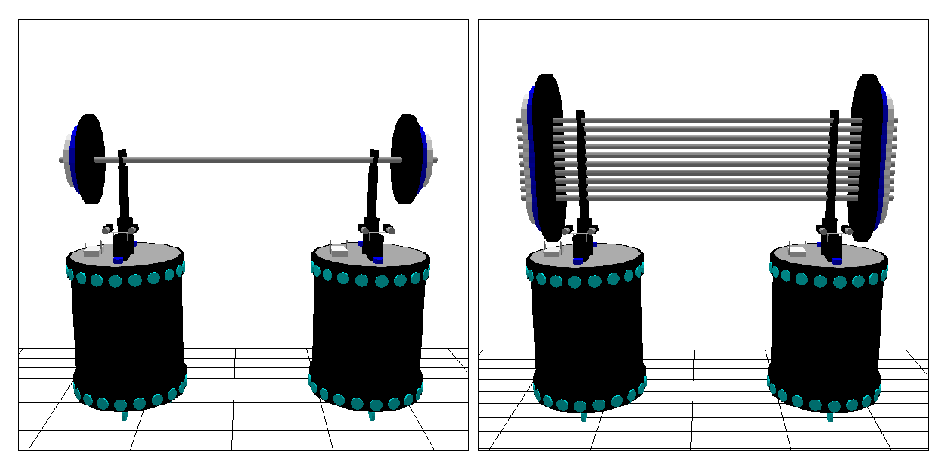
\includegraphics[width=10cm]{FIG/Constraint/halteres.eps}
}
\centerline{
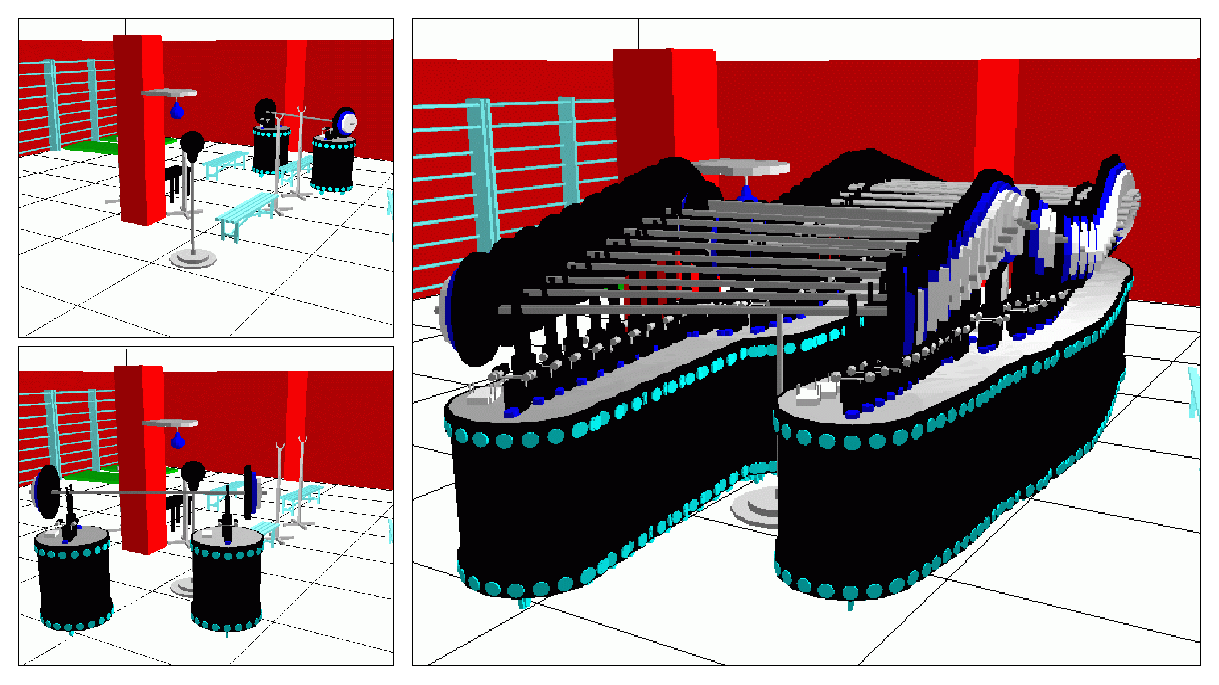
\includegraphics[width=10cm]{FIG/Constraint/halteres2.eps}
}
\caption{\label{fig:halteres} Two holonomic robots cooperating in a
task. The bar with the weighs must stay horizontal, so the hydraulic
bars of the robots must move at the same time.}
\end{figure}


Another example of application of this kinematic constraint would be
the incorporation of natural effects in the simulating model. The
constraint represented in Figure~\ref{fig:dedos} corresponds to the
natural motion of a finger. There is a relationship between the
movement of the phalanges of a hand finger. It could be modeled in a
simple way as a linear relationship.

\begin{figure}[ht!]
%\vspace{15.0mm}
\begin{center}
  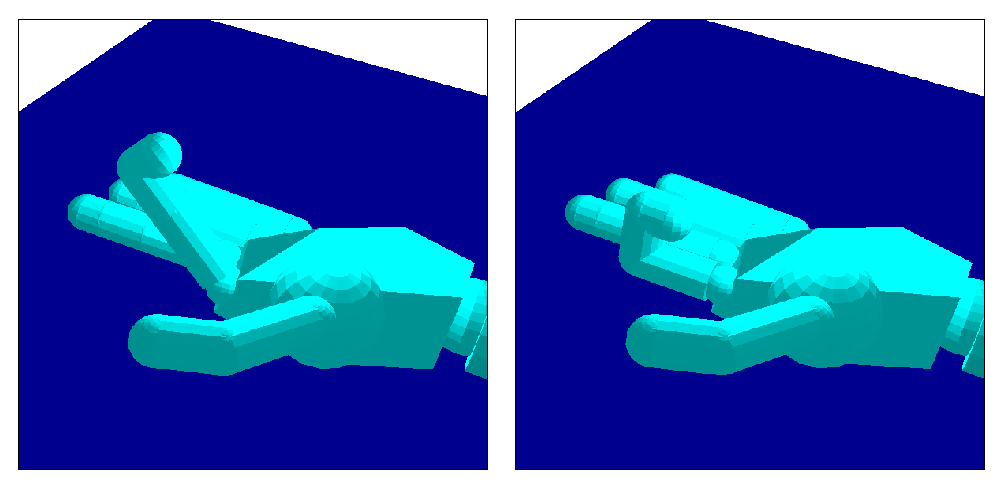
\includegraphics[width=10.0cm]{FIG/Constraint/dedos.eps}
\end{center}
\caption{\label{fig:dedos} Constraint in the movement of a finger. The 
left figure shows an abnormal position for a finger, the right one shows a 
normal situation.}
%\vspace{5.0mm}
\end{figure}


\subsection*{$RRPR$, $4R$ and $3RPR$ linkages}

The $RRPR$, $4R$ nd $3RPR$ linkages are basic planar closed kinematic
chains. Theirs constraint equations are calculated by planar geometry,
likewise theirs motion limits. It must be remarked that {\bf joints
  affected by these constraints must be defined on the same plane}.
Next each one of these linkages will be separately explained.

%\vspace{5.0mm}
\begin{figure}[ht!]
%\vspace{5.0mm}
\begin{center}
\psfrag{teta}[l]{$\theta$} 
\psfrag{chi}[l]{$\psi$}
\psfrag{r}[l]{$r$}
\psfrag{s}[l]{$s$}
\psfrag{g}[l]{$g$}
\psfrag{e}[l]{$e$}
  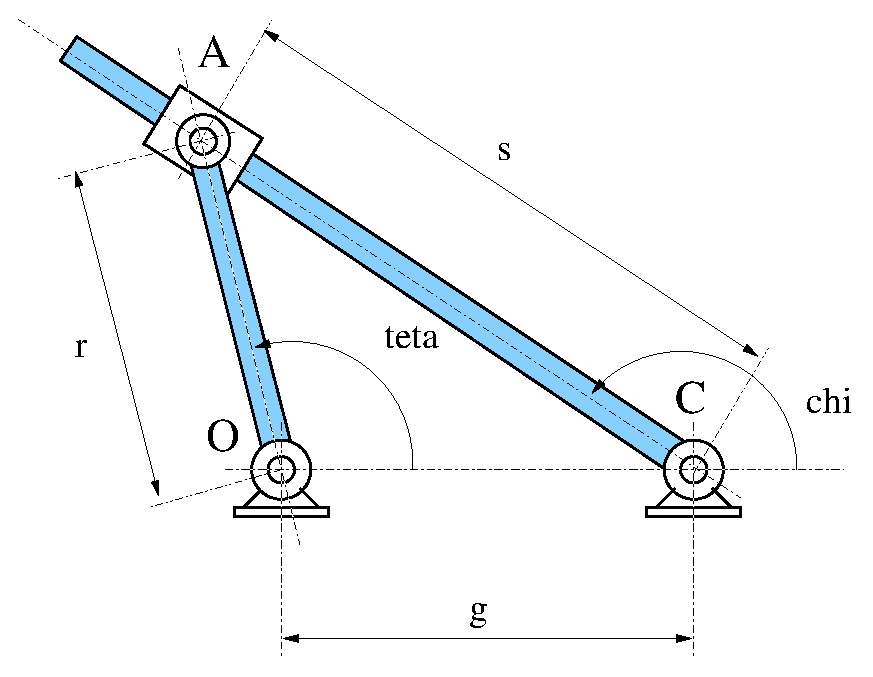
\includegraphics[width=7.0cm]{FIG/Constraint/RRPR2.eps}
\end{center}
\caption{\label{fig:RRPR} The dimensions characterizing an $RRPR$
linkage.}
%\vspace{5.0mm}
\end{figure}


The $RRPR$ linkage is known as a {\em slider-crank} and consist of two
rotating cranks linked by a translating slider. It is a one
degree-of-freedom planar closed chain that is a fundamental machine
element found in everything from automotive engines to door closing
mechanisms.

In the implementation of this constraint in Move3D, the
translation $s$ has been chosen to be the d.o.f. that controls the chain. Therefore,
the joint representing $s$ ($JA$) will be the active joint and the joints
representing $\theta$ ($JO$) and $\psi$ ($JC$) will be the passive
ones. Notice that $JO$ and $JC$ must have the same parent, and $JA$
must be placed in the point corresponding to {\bf A} in the modeling.

\begin{figure}[ht!]
\begin{center}
\psfrag{teta}[l]{$\theta$} 
\psfrag{chi}[l]{$\psi$}
\psfrag{fi}[l]{$\phi$}
\psfrag{a}[l]{$a$}
\psfrag{h}[l]{$h$}
\psfrag{g}[l]{$g$}
\psfrag{b}[l]{$b$}
 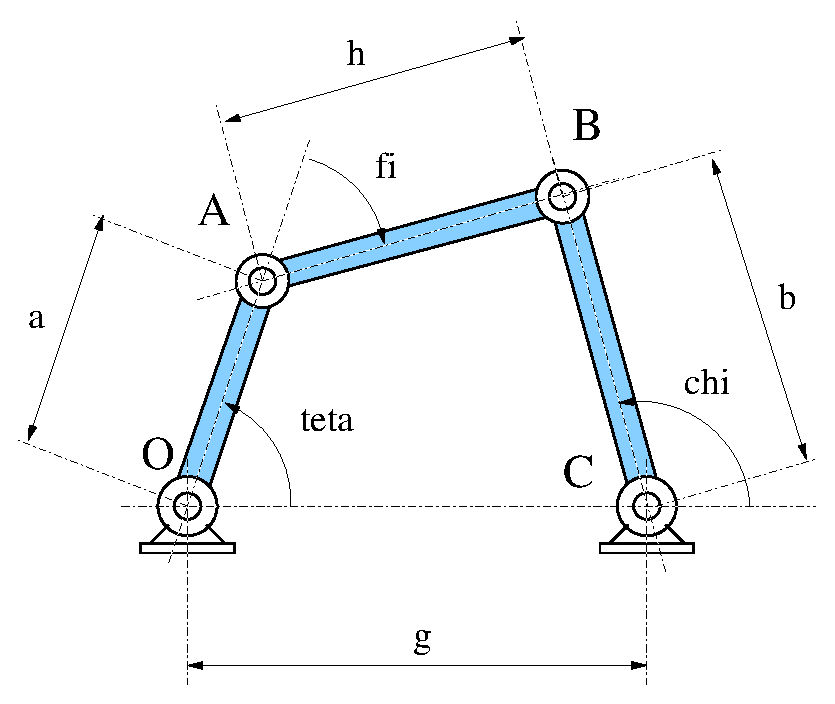
\includegraphics[width=7.0cm]{FIG/Constraint/4R.eps}
\end{center}
\caption{\label{fig:4R} The dimensions characterizing an $4R$ linkage.}
\end{figure}

The $4R$ linkage is a four-rotations planar closed chain. It consist
of an input crank ({\bf OA}), an output crank ({\bf CB}) and a coupler 
({\bf AB}). There is also just one d.o.f. in this fundamental mechanism,
which is the input crank.  

The following remarks must be obeyed for the modeling of this chain:
$JO$ and $JC$ must be defined on the same solid; the coupler must be
defined from the input crank, that is, the chain is cut at {\bf B};
the joint $JB$ can be placed at the end of the output crank or at the
end of the coupler, but this joint is necessary in order to calculate
lengths of the links.

The $3RPR$ linkage can be seen as a $4R$ linkage where the length of
the output crank is variable. It is, therefore, a two d.o.f. planar
closed chain. These two active joints corresponds to the input crank
({\bf OA}) and the translating slider placed at {\bf B} on the output
crank. 

\begin{figure}[ht!]
\begin{center}
\psfrag{teta}[l]{$\theta$} 
\psfrag{chi}[l]{$\psi$}
\psfrag{fi}[l]{$\phi$}
\psfrag{a}[l]{$a$}
\psfrag{h}[l]{$h$}
\psfrag{g}[l]{$g$}
\psfrag{s}[l]{$s$}
 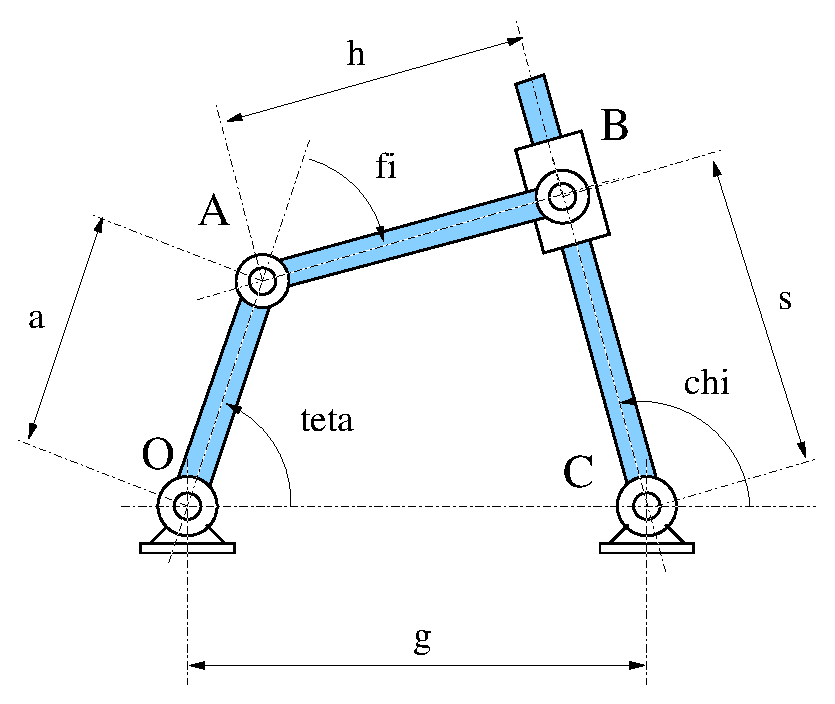
\includegraphics[width=7.0cm]{FIG/Constraint/3RPR.eps}
\end{center}
\caption{\label{fig:3RPR} The dimensions characterizing an $3RPR$ linkage.}
\end{figure}

The remarks for the modeling are similar to the ones made for the
$4R$ linkage, but in this case $JB$ is the translating joint, and it
must be defined from the output crank.

Now, some of the results obtained before the
implementation of these constraints in Move3D will be shown. Figures~\ref{fig:excavator}
represents the model of an hydraulic excavator. The motion of its arm
is controlled by the hydraulic systems, so there are 3 d.o.f.. This
mechanical system contains four closed kinematic chains. Three of them
are the hydraulic systems, and the fourth one is the mechanism for the
motion of the bucket. The hydraulic systems can be modeled as $RRPR$
linkages where the translating crank is the hydraulic bar. The
mechanism of the bucket is a $4R$ linkage. But the third hydraulic
system and the mechanism of the bucket are linked, so we really have
two single closed chains and one double loop closed chain.

\begin{figure}[hb!]
\begin{center}
  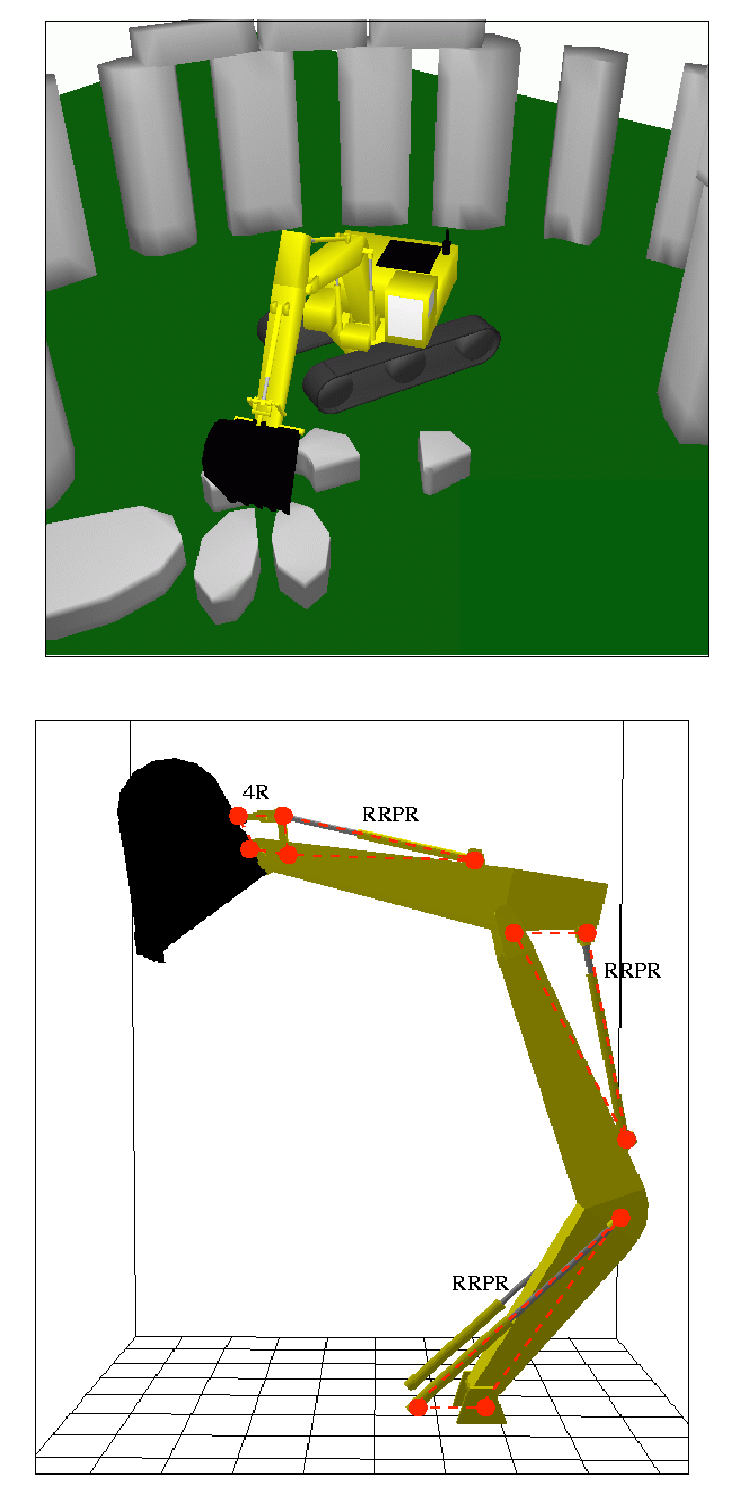
\includegraphics[width=8.1cm]{FIG/Constraint/excavator.eps}
\end{center}
\caption{\label{fig:excavator} Hydraulic excavator. This model
contains two single closed chains and one double loop closed chain. The 
arm, a mechanical system of 19 d.o.f. has been constrained to a system of 3 d.o.f..}
\end{figure}


\begin{figure}[ht!]
\begin{center}
  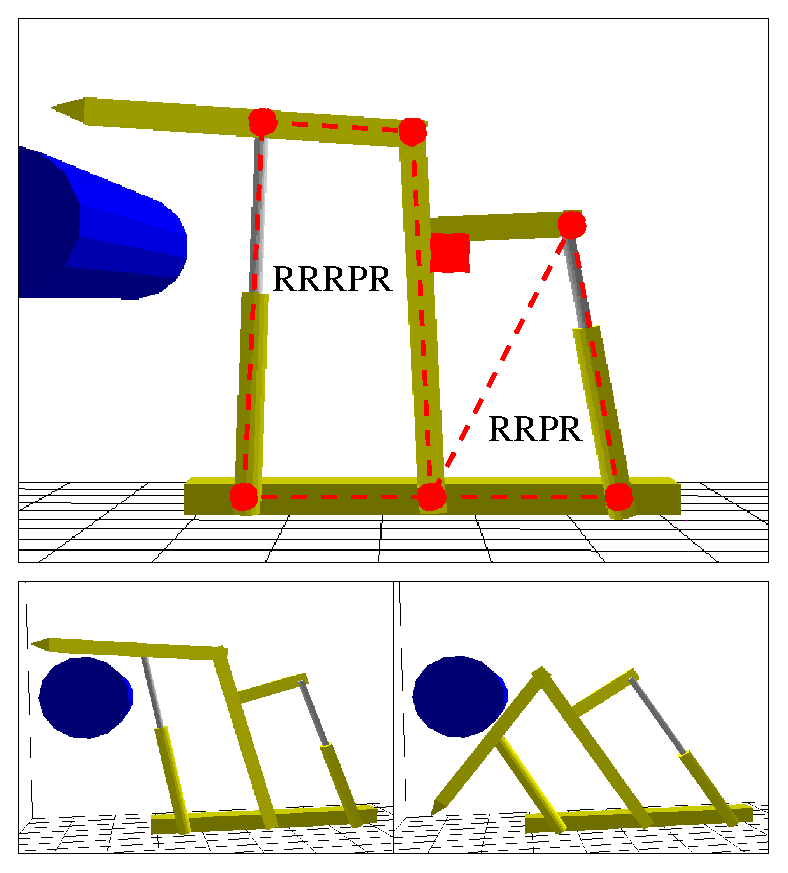
\includegraphics[width=8.0cm]{FIG/Constraint/liegeois.eps}
\end{center}
\caption{\label{fig:liegeois} Manipulator shown in some works of Liegeois.
This two d.o.f. mechanical system consist of a double loop closed chain.} 
\end{figure}

The mechanical system in Figures~\ref{fig:liegeois} is another example
of a double loop closed chain. In this case, the two single chains are 
a $RRPR$ linkage for the rear hydraulic system, and a $3RPR$ linkage
for the front loop.


\subsection*{Contact with ground}

This kinematic constraint represents the case when an object is
required to stay in contact with an obstacle. Particularly, the
implemented constraint corresponds to an object that have to move with
its lowest point sliding on the ground.

The kind of problems which we are mainly interested in are mobile
machines (robots) carrying long objects that have to trail on the
ground. However, the general problem has not been already solved. Just
the last joint of the robot, that is, the joint of the terminal organ
of the robot which grasp the carried object, is going to be
controlled.  This joint must be a revolute joint turning around an
axis perpendicular to the absolute $z$-axis of the scene. This
particular case can be seen as a planar problem.

\begin{figure}[ht!]
\begin{center}
\psfrag{te}[l]{$\theta$} 
\psfrag{li}[l]{$\theta_{JC}$}
\psfrag{de}[l]{$\theta o_{JC}$}
\psfrag{ang}[l]{$\theta_{Object}$}
\psfrag{ant}[l]{$\theta_P$}
\psfrag{d}[l]{$d$}
\psfrag{z_J}[l]{$z_J$} 
\psfrag{z_G}[l]{$z_0$}    
  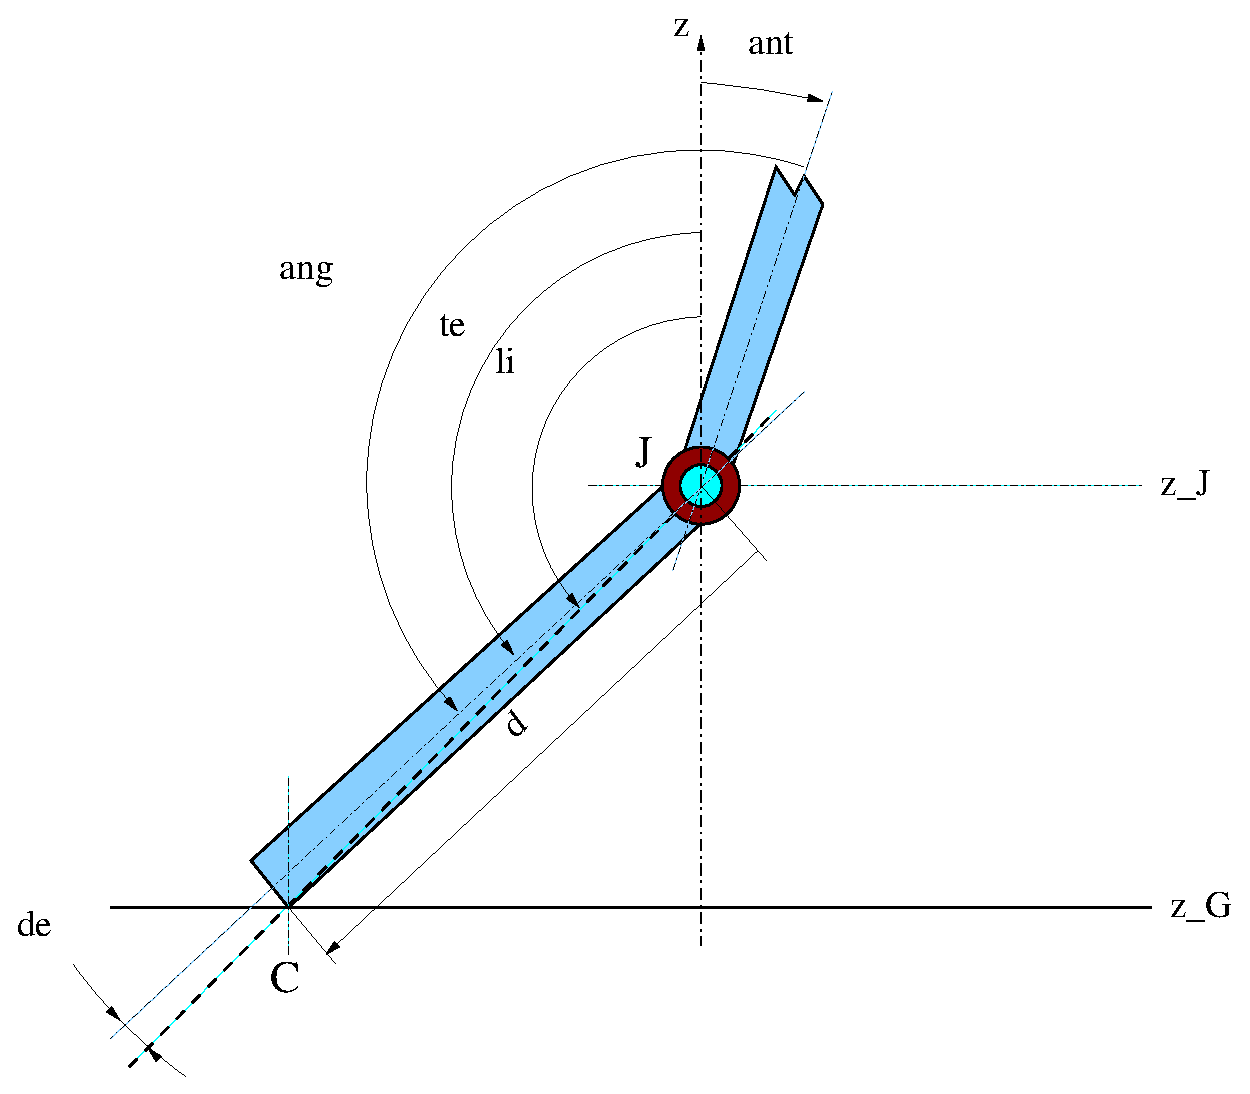
\includegraphics[width=7cm]{FIG/Constraint/ground.eps}
\end{center}
\caption{\label{fig:ground} Variables and references in the analysis.}
\end{figure}

Some remarks for the modeling must be made for this constraint. Let us 
suppose that, for long-shaped objects, the point having to stay
in contact with the ground does not change. In the file containing the
workspace for the path planning with Move3D, the carried object must
be modeled as another body of the robot. Therefore, a joint can be
placed in the point of this `body' that has to slide on the ground.
This joint will be or not a connection with another body, so it will
be not a real joint, but it is necessary to include it in the model.
Let us call it {\bf $J_C$} because it is placed at the point {\bf C}.
It must not be forgotten during the modeling that we are solving a
planar problem. That is to say that the points {\bf J} and {\bf $J_C$}
must be in the same plane, and this plane must be perpendicular to the
rotation axis of the joint at {\bf J}.

\begin{figure}[ht!]
\begin{center}
  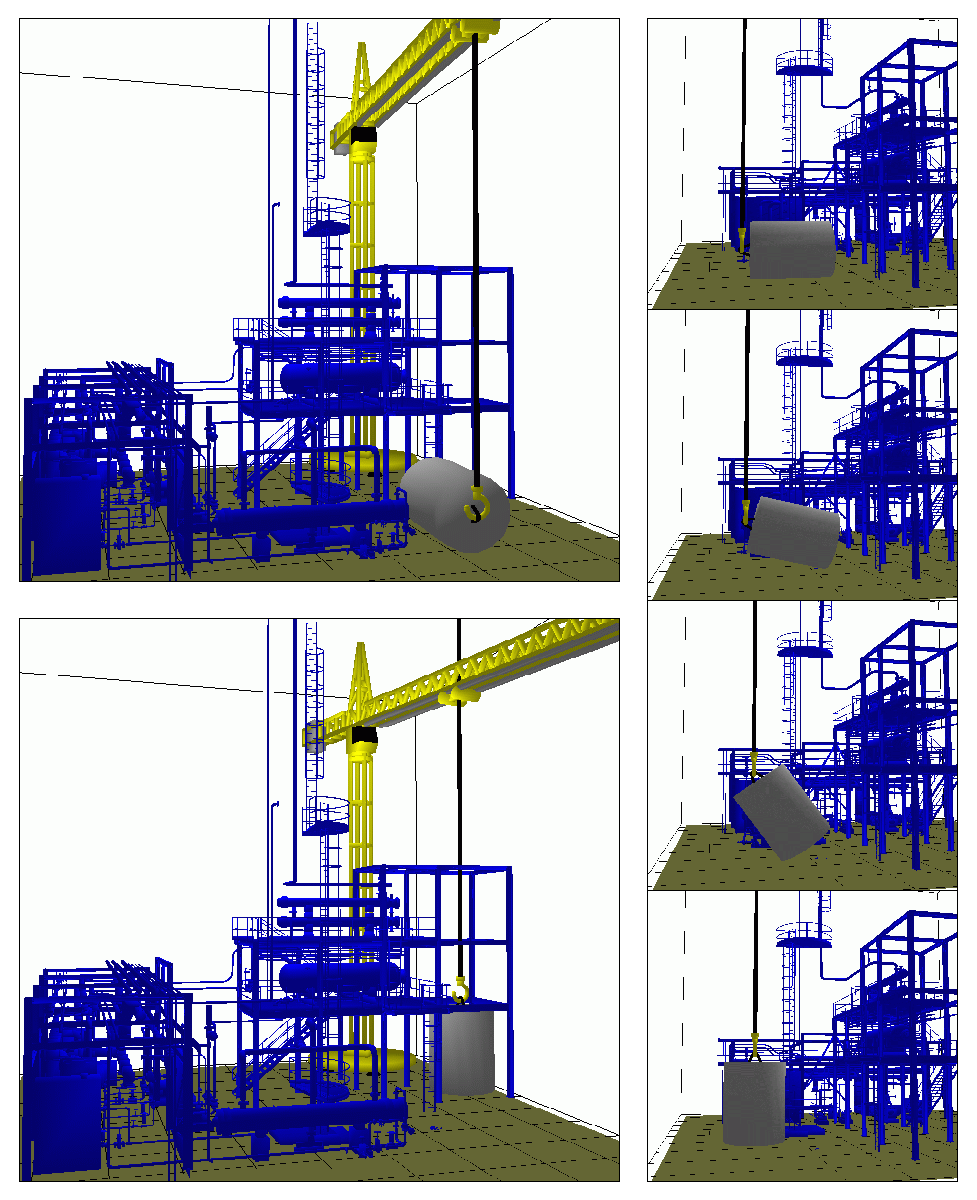
\includegraphics[width=8.0cm]{FIG/Constraint/grue.eps}
\end{center}
\caption{\label{fig:gruaind} A crane has to place a tank into a
metallic structure in an industrial environment. In the initial
configuration, the tank is horizontally placed on the ground. The tank
has to slide on the ground before it reaches the vertical position.}
\end{figure}

Applications of this kind of kinematic constraint are particularly
interesting. For instance, in industrial environments they exist path
planning problems where a moving object must stay in contact with the
ground following physical laws. Figure~\ref{fig:gruaind} shows an
example of one of these problems. The typical example of application,
also usual in the industrial environments, consist in a `robot'
carrying long-shaped objects with a point sliding on the ground. The
example in Figure~\ref{fig:pipe} shows the performance of the planner
handling this kind of kinematic constraint.

\begin{figure}[ht!]
\centerline{
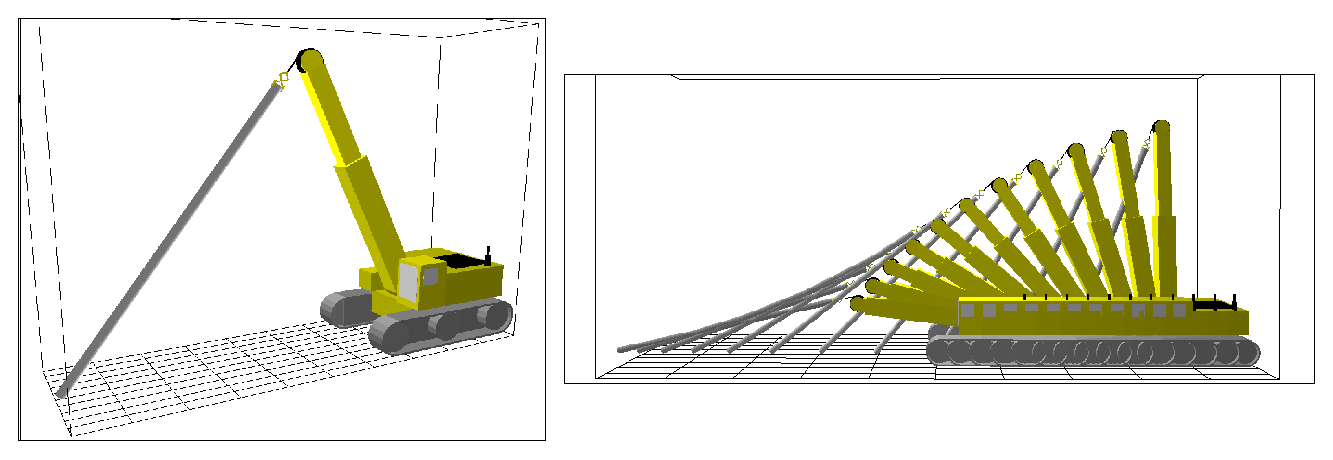
\includegraphics[width=15cm]{FIG/Constraint/pipe12.eps}
}
\caption{\label{fig:pipe} A telescopic handler carries a long
pipe. The lowest extreme of the pipe must stay in contact with the
ground all along the path.}
\end{figure}

\subsection*{Car front wheels}

\begin{figure}[ht!]
\begin{center}
\psfrag{t}[l]{$\theta$} 
\psfrag{O}[l]{O} 
\psfrag{P}[l]{P}    
  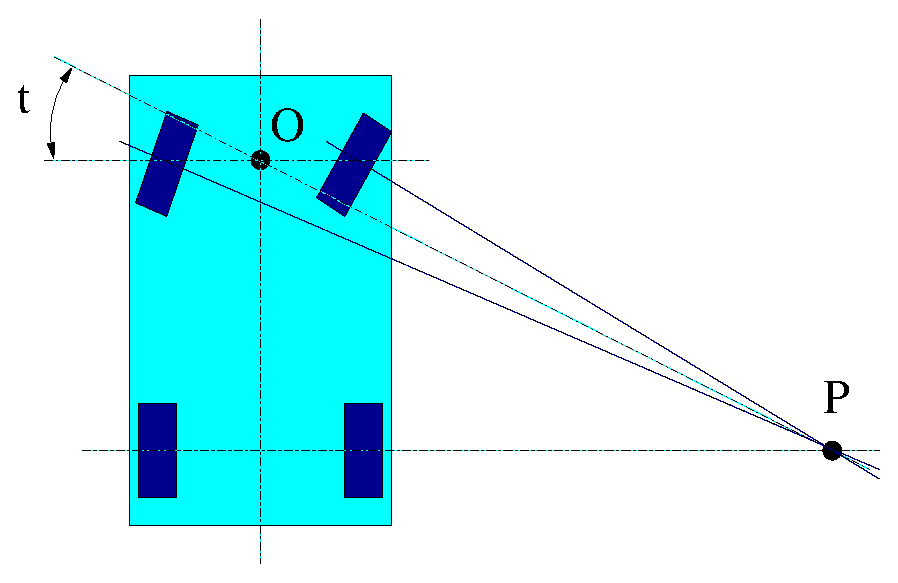
\includegraphics[width=8cm]{FIG/Constraint/carfw.eps}
\end{center}
\caption{\label{fig:carfw} Geometric law for the angles of the car 
  front wheels.}
\end{figure}

This kinematic constraint will be applied to cars. A car can be
modeled as a robot towing a trailer. The steering column of the car is
represented by the robot and the body of the car is represented by the
trailer (see Chapter~\ref{methode-local}). The angle of each
front wheel is then computed as shown on Figure~\ref{fig:carfw}.
That is, the axes of all the wheels (front and rear) must coincide in
a same point {\bf P}.  This point is also the intersection between the
rear wheels axis and the line passing trough the car turning center
(steering column) {\bf O} and having the car turning angle $\theta$.
This point {\bf O} represents the joint between the robot and the
trailer.

Figure~\ref{fig:LegoCar} shows the model of a car
within this constraint has been successfully tried.



\begin{figure}[htb!]
\begin{center}
  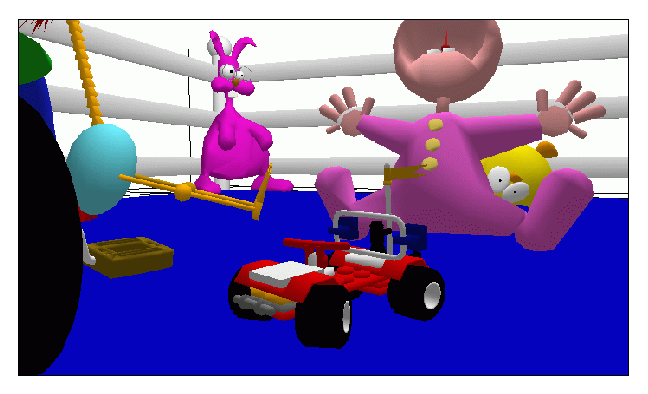
\includegraphics[width=8cm]{FIG/Constraint/LegoCar.eps}
\end{center}
\caption{\label{fig:LegoCar} Three-dimensional model of a LegoCar.}
\end{figure}


\subsection*{Planar closed chain}

A general analytical solution for a planar closed
chain is used in this constraint. It is known that for a n-bar planar mechanism, the number of
d.o.f is n-3. The base of the mechanical system is considered as one
of the bars, then it becomes a (n-1)-bar mechanism with (n-1)-2 d.o.f.
The chosen method to solve this geometrical problem
consist of cutting the loop in two parts. At one side we leave a 2-bar
open chain. At the other side we will have another open chain with the
rest of the elements. The two joints of the first part will be the
passive joints (the two lost d.o.f.), while the joints the other part
remain active. The angles of the passive joints are calculated by
trigonometric laws in order to close the loop.

\begin{figure}[h!]
\begin{center}
\psfrag{a}[l]{$\theta 1$} 
\psfrag{b}[l]{$\theta 2$}
\psfrag{chi}[l]{$\psi$}
\psfrag{fi}[l]{$\phi$}
\psfrag{d}[l]{$d$}
\psfrag{any planar open chain}[l]{any planar open chain}
  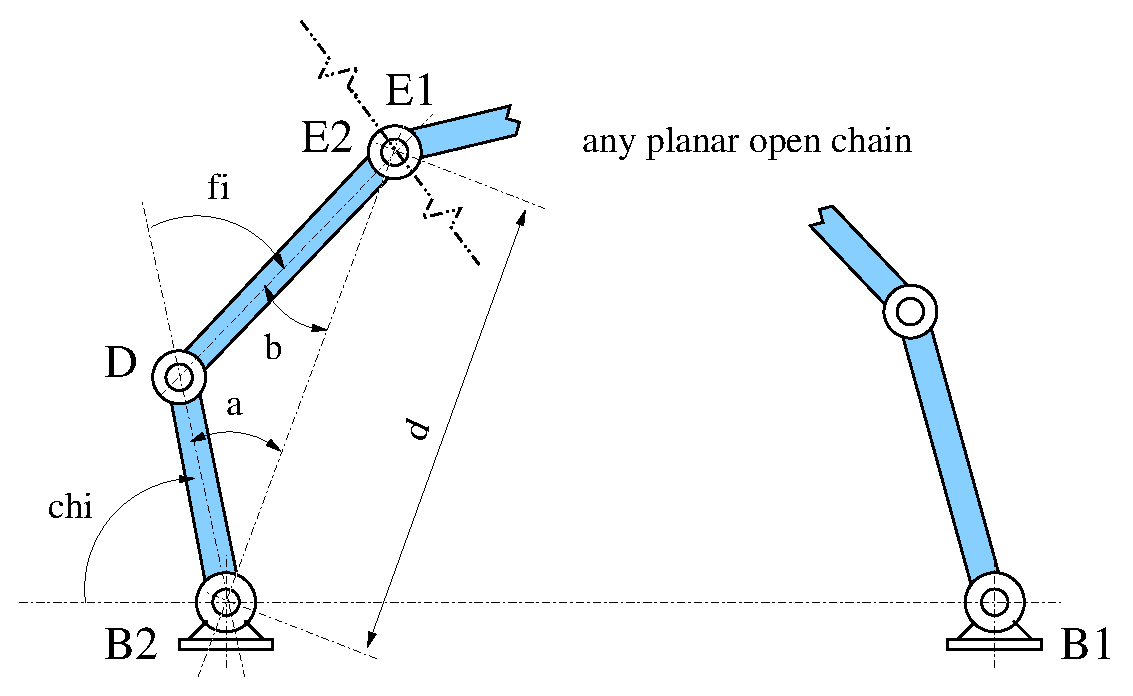
\includegraphics[width=7cm]{FIG/Constraint/plclch.eps}
\end{center}
\caption{\label{fig:plclch} Variables and references in the analysis.}
\end{figure}

Figure~\ref{fig:plclch} represents the way how a mechanical system 
containing this kinematic constraint must be modeled. Joints ({\bf E1}
and {\bf E2}) must be placed at the end of each open chain.

Figure~\ref{fig:cad8pas} shows the performance of Move3D solving a 
path planning problem for a 8-bar closed chain.

\begin{figure}[h!]
\begin{center}
  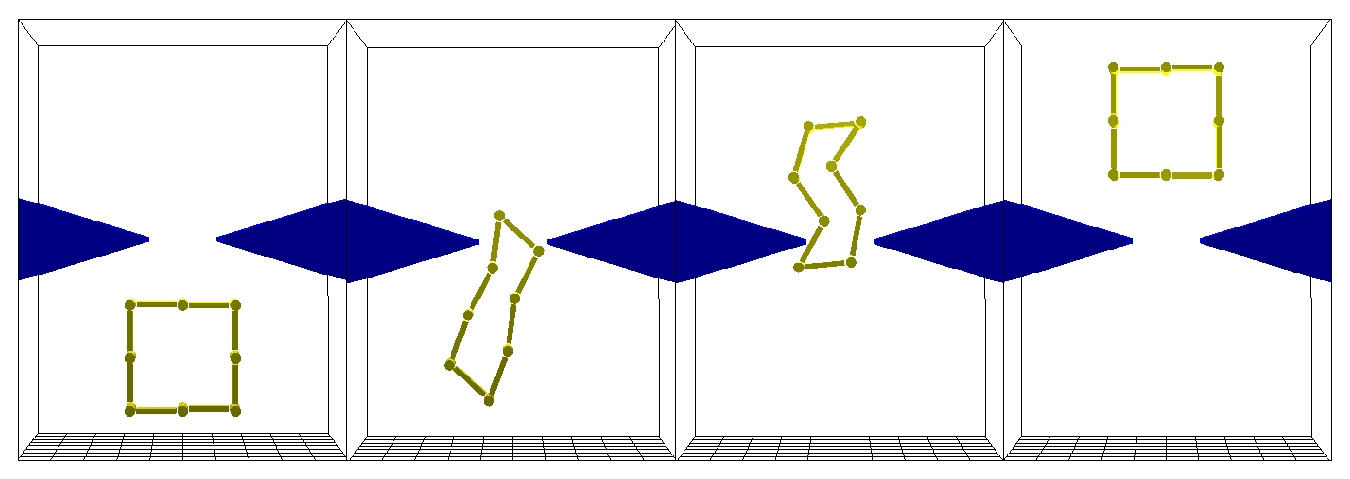
\includegraphics[width=10cm]{FIG/Constraint/cad8pas.eps}
\end{center}
\caption{\label{fig:cad8pas} Some sequences of the solution given
  by Move3D for a 8-bar closed chain that has to find a path trough a
  narrow passage.}
\end{figure}

\section{How to use them}

Kinematic constraints can be set in the mechanical system in two ways: 
they can be directly set in the model input file ({\tt .p3d}), or they can
be set once Move3D is running. Next, this two
possibilities are explained.

\subsection*{Kinematic constraints in the {\tt .p3d} file}

Constraints can be introduced in the mechanical system by adding command 
lines at the end of the model input file. These command lines have the 
following structure: 

\hspace{-4.0mm}
{\tt p3d\_constraint \footnotesize cntrt\_name npasjnts \{pj1...pjn\} nactjnts
  \{aj1...ajn\} nc \{c1...cn\} no \{o1...on\}} \index{p3d\_constraint} \\

where:
\begin{tabbing}
>>>\=>>>>>>>>>>>>> \= \kill
\> - {\tt cntrt\_name} \>: is the name of the kinematic constraint to 
  be set.\\
\> - {\tt npasjnts}   \>: is the number of passive joints.\\
\> - {\tt \{pj1...pjn\}}\>: are the indexes corresponding to each one of 
  the passive joints.\\
\> - {\tt nactjnts}   \>: is the number of active joints.\\
\> - {\tt \{aj1...ajn\}}\>: are the indexes corresponding to each one of 
  the active joints.\\
\> - {\tt nc}         \>: is the number of (real) constant parameters.\\
\> - {\tt \{c1...cn\}}  \>: are the constant parameters of the
  constraint.\\
\> - {\tt no}          \>: is the number of other (integer) constant parameters.\\
\> - {\tt \{o1...on\}}   \>: are integer constant parameters of the
  constraint.\\
\end{tabbing}

  
For each one of the kinematic constraints explained in
the last section, the parameters of this command line are as follows
(see figures in last section for the references of points and joints):

\begin{tabbing}
>\=>>\=>>>>>>>>>>>>\=>>>\= \kill
\>{\normalsize \bf Linear relationship between two d.o.f.} \\
\>\>\\
\>\>{\bf \tt cntrt\_name} \>: {\tt p3d\_lin\_rel\_dofs}\\
\>\>{\bf \tt npasjnts} \>: 1\\
\>\>{\bf \tt pj1} \>: index of the joint to be controlled ($JA$)\\
\>\>{\bf \tt nactjnts} \>: 1\\
\>\>{\bf \tt aj1} \>: index of the joint that controls $JA$ ($JB$)\\
\>\>{\bf \tt nc} \>: 2\\
\>\>{\bf \tt c1} \>: linear relationship coefficient ($K$)\\
\>\>{\bf \tt c2} \>: offset ($C$)\\
\>\>{\bf \tt no} \>: 0\\
\>\>\\
\>{\normalsize \bf $RRPR$ linkage} \\
\>\>\\
\>\>{\bf \tt cntrt\_name} \>: {\tt p3d\_RRPRlnk}\\
\>\>{\bf \tt npasjnts} \>: 2\\
\>\>{\bf \tt pj1} \>: index of the joint corresponding to {\bf O}\\
\>\>{\bf \tt pj2} \>: index of the joint corresponding to {\bf C}\\
\>\>{\bf \tt nactjnts} \>: 1\\
\>\>{\bf \tt aj1} \>: index of the translating joint, placed at {\bf A}\\
\>\>{\bf \tt nc} \>: 0\\
\>\>{\bf \tt no} \>: 0\\
\>\>\\
\>{\normalsize \bf $4R$ linkage} \\
\>\>\\
\>\>{\bf \tt cntrt\_name} \>: {\tt p3d\_4Rlnk}\\
\>\>{\bf \tt npasjnts} \>: 3\\
\>\>{\bf \tt pj1} \>: index of the joint corresponding to {\bf A}\\
\>\>{\bf \tt pj2} \>: index of the joint corresponding to {\bf B}\\
\>\>{\bf \tt pj3} \>: index of the joint corresponding to {\bf C}\\
\>\>{\bf \tt nactjnts} \>: 1\\
\>\>{\bf \tt aj1} \>: index of the joint corresponding to {\bf O}\\
\>\>{\bf \tt nc} \>: 0\\
\>\>{\bf \tt no} \>: 0\\
\>\>\\
\>{\normalsize \bf $3RPR$ linkage} \\
\>\>\\
\>\>{\bf \tt cntrt\_name} \>: {\tt p3d\_3RPRlnk}\\
\>\>{\bf \tt npasjnts} \>: 2\\
\>\>{\bf \tt pj1} \>: index of the joint corresponding to {\bf A}\\
\>\>{\bf \tt pj2} \>: index of the joint corresponding to {\bf C}\\
\>\>{\bf \tt nactjnts} \>: 2\\
\>\>{\bf \tt aj1} \>: index of the joint corresponding to {\bf O}\\
\>\>{\bf \tt aj2} \>: index of the translating joint, placed at {\bf B}\\
\>\>{\bf \tt nc} \>: 0\\
\>\>{\bf \tt no} \>: 0\\
\>\>\\
\>{\normalsize \bf Contact with ground} \\
\>\>\\
\>\>{\bf \tt cntrt\_name} \>: {\tt p3d\_jnt\_on\_ground}\\
\>\>{\bf \tt npasjnts} \>: 1\\
\>\>{\bf \tt pj1} \>: index of the joint sliding on the ground ($J_C$)\\
\>\>{\bf \tt nactjnts} \>: 0\\
\>\>{\bf \tt nc} \>: 2\\
\>\>{\bf \tt c1} \>: height ($z$) of the ground\\
\>\>{\bf \tt c2} \>: offset with relation to the horizontal plane
when the body is hanging\\
\>\>{\bf \tt no} \>: 3  (for these variables: 0 == OFF, 1 == ON)\\
\>\>{\bf \tt o1} \>: $J_C$ turns in the negative direction\\
\>\>{\bf \tt o2} \>: $J_C$ changes the turning direction depending on
the position of the rest\\\>\>\>\> of bodies of the robot\\
\>\>{\bf \tt o3} \>: the carried body must stay on the ground (it can
not be hung)\\
\>\>\\
\>{\normalsize \bf Car front wheels} \\
\>\>\\
\>\>{\bf \tt cntrt\_name} \>: {\tt p3d\_car\_front\_wheels}\\
\>\>{\bf \tt npasjnts} \>: 2\\
\>\>{\bf \tt pj1} \>: index of the joint corresponding to the right wheel\\
\>\>{\bf \tt pj2} \>: index of the joint corresponding to the left wheel\\
\>\>{\bf \tt nactjnts} \>: 1\\
\>\>{\bf \tt aj1} \>: index of the joint corresponding to the steering
column {\bf O}\\
\>\>{\bf \tt nc} \>: 2\\
\>\>{\bf \tt c1} \>: distance between front and rear wheels axes\\
\>\>{\bf \tt c2} \>: distance between front wheels\\
\>\>{\bf \tt no} \>: 0\\
\>\>\\
\>{\normalsize \bf Planar closed chain} \\
\>\>\\
\>\>{\bf \tt cntrt\_name} \>: {\tt p3d\_planar\_closed\_chain}\\
\>\>{\bf \tt npasjnts} \>: 2\\
\>\>{\bf \tt pj1} \>: index of the last joint of the controllable (active) half-chain {\bf E1}\\
\>\>{\bf \tt pj2} \>: index of the last joint of the non-controllable (passive) half-chain {\bf E2}\\
\>\>{\bf \tt nactjnts} \>: 1\\
\>\>{\bf \tt aj1} \>: index of the first joint of the controllable half-chain {\bf B1}\\
\>\>{\bf \tt nc} \>: 0\\
\>\>{\bf \tt no} \>: 0\\
\end{tabbing}


\subsection*{Setting and modification of constraints while Move3D is running}

The access to the kinematic constraints, while Move3D is running, is
got from the so called button in the robot control window. This button 
generates the {\em kinematic constraints window} (see
Figure~\ref{fig:kcwin}). This window allows the user to manage
three operations:

\begin{figure}[b!]
\begin{center}
  \includegraphics[width=7.9cm]{FIG/Constraint/kcwin.ps}
\end{center}
\caption{\label{fig:kcwin} Kinematic constraints window. In this
  case, the list of constraints corresponds to the model of the
  excavator arm (see Figure~\ref{fig:excavator}).}
\end{figure}

\begin{itemize}
\item {\bf Activation and deactivation of constraints :} \\
Buttons placed at the left on the kinematic constraints window allow
to activate (pushed) or deactivate (released) any of the already set
constraints. It is important to remark at this point that two kinematic
constraints having the same passive joints can not be active at the
same time.
\item {\bf Modification of some of the parameters of constraints:} \\
A window containing the parameters of each one of the listed constrains 
appears by pushing its corresponding button at the right of the
kinematic constraints window. In this window, the user can modify
some of the parameters of the constraint. Parameters related to joints 
indexes are forbidden to be changed. Upper part of Figure~\ref{fig:jogwins}
represents an example of these windows.
\item {\bf Setting of new constraints:} \\
Kinematic constraints non-included in the model input file can be
introduced in the mechanical system during the running of Move3D. The
{\em kinematic constraints setting window} appears by pushing the button
``NEW'' on the kinematic constraints window. This window contains the 
list of the kinematic constraints types treated in Move3D. Buttons
placed at the right on this window generate the setting windows of
each one of them. The parameters appearing in these setting windows
have been explained in Section ``Treated constraints''. New
constraints containing wrong parameters will not be set, and an error
message will be displayed. Bottom part of Figure~\ref{fig:jogwins} illustrates
the process for a new constraint setting.
\end{itemize}

\begin{figure}[h!]
\begin{center}
  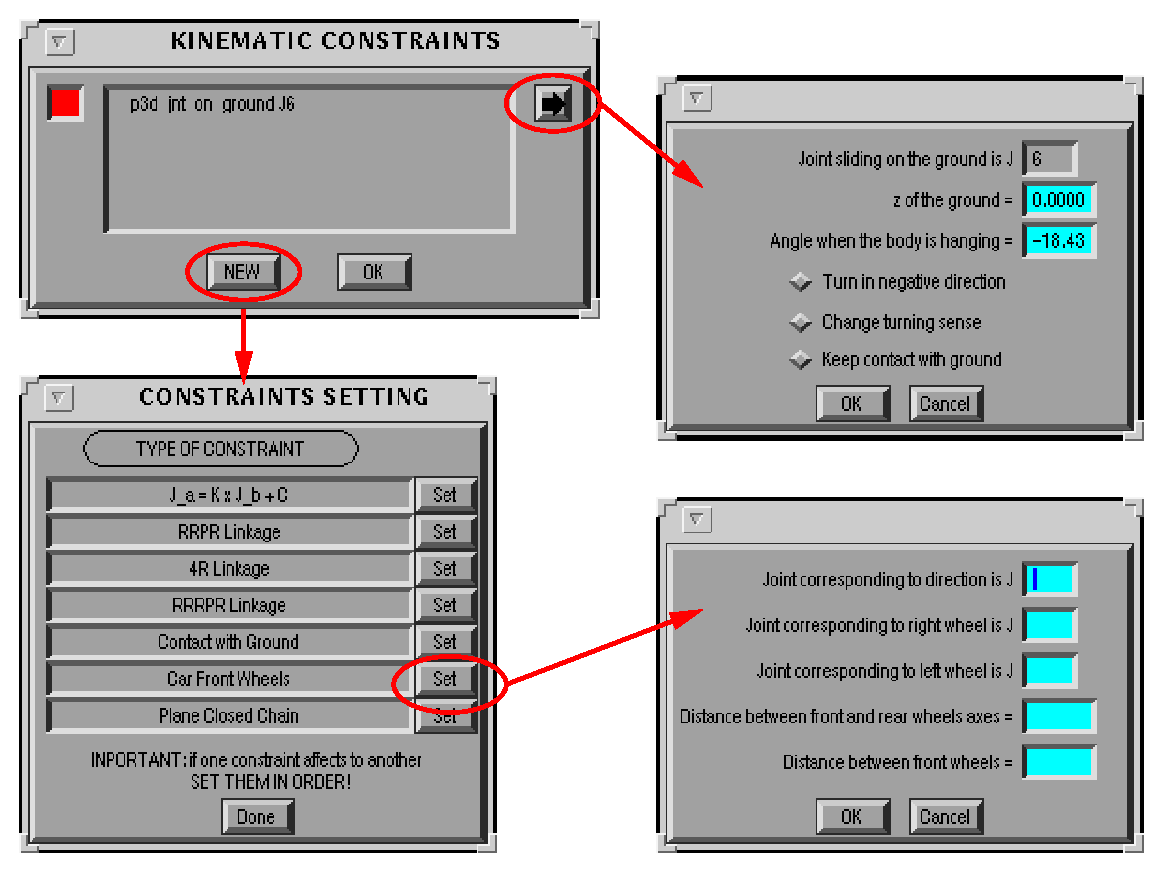
\includegraphics[width=14.0cm]{FIG/Constraint/jogwins.eps}
\end{center}
\caption{\label{fig:jogwins} Kinematic constraints window, kinematic
  constraints setting window, window containing the parameters of a
  constraint and setting window of a constraint.}
\end{figure}
 

\section{Implementation}

When a kinematic constraint is set, its data structure is
generated. This data structure contains all the necessary information
for the treatment of the constraint. The representation in C language
of this structure is:
{\tt
\begin{tabbing}
>>>>>>>>>>>>\=>>\=>>>>>>>>>>>> \= \kill
\>typedef struct cntrt \{ \\ 
\>\>  int       \> num;\\
\>\>  char      \> namecntrt[40];\\
\>\>  int       \> active;\\
\>\>  int       \> (*fct\_cntrt)(struct cntrt *ct);\\
\>\>  int       \> nactjnts, npasjnts;\\
\>\>  int       \> ndval, nival;\\
\>\>  int       \> actjnts[MAX\_ARGU\_CNTRT];\\
\>\>  int       \> actjnt\_state[MAX\_ARGU\_CNTRT];\\
\>\>  int       \> pasjnts[MAX\_ARGU\_CNTRT];\\
\>\>  int       \> argu\_i[MAX\_ARGU\_CNTRT];\\
\>\>  double    \> argu\_d[MAX\_ARGU\_CNTRT];\\
\>\>  int       \> col\_pairs[2][MAX\_ARGU\_CNTRT];\\
\>\>  struct cntrt \> *next\_cntrt;\\
\>\>  struct cntrt \> *prev\_cntrt;\\
\>\>  int       \> enchained\_J[MAX\_ARGU\_CNTRT];\\
\>\>  int       \> nenchained;\\
\>\>  struct cntrt \> **enchained;\\
\>\} p3d\_cntrt,*pp3d\_cntrt; \\
\end{tabbing}
}

Some of the members of this data structure have been already
named, and theirs values are directly given by the user. The rest
of them are automatically calculated in the setting function of each
constraint. In order to  allow a further comprehension about how the
implementation of the kinematic constraints is made, these variables
will be briefly explained next.
\begin{itemize}
\item[$-$] The data structure of each robot in the workspace of Move3D contains 
an array of pointers to the data structures of its kinematic
constraints. {\bf \tt num} represents the index of a constraint in this
list.
\item[$-$] {\bf \tt name} contains the name of the constraint.
\item[$-$] {\bf \tt active} is a flag to indicate the state of the constraint
 (activated/deactivated).
\item[$-$] {\bf \tt fct\_cntrt} is a pointer to the function
containing the equations to solve this constraint type.
\item[$-$] {\bf \tt nactjnts} and {\bf \tt npasjnts} are respectively the number
  of active and passive joints of the constraint.
\item[$-$] {\bf \tt ndval} and {\bf \tt nival} are respectively the
  number of real and integer constant parameters of the constraint
  that are given by the user.
\item[$-$] {\bf \tt actjnts} and {\bf \tt pasjnts} are arrays containing the indexes of 
the active and passive joints in this constraint.
\item[$-$] {\bf \tt actjnt\_state} is an array of flags for the active joints of
the constraint. A flag set to $0$ means that the corresponding joints
is involved in a previously defined constraint.
\item[$-$] {\bf \tt argu\_i} and {\bf \tt argu\_d} contain respectively integer and
real constant parameters of the kinematic constraint. Some of these
parameters are the ones introduced by the user. The rest are
automatically calculated. The kind of these calculated constants are, for
example: flags, distances between joints or values to refer angles.
\item[$-$] {\bf \tt col\_pairs} is used to stock information for the 
  deactivation of pairs of bodies for the collision checking.
\item[$-$] {\bf \tt next\_cntrt} and {\bf \tt prev\_cntrt} are
  pointers to the next and preceding constraints in the above
  mentioned list.
\item[$-$] {\bf \tt enchained\_J}, {\bf \tt nenchained} and {\bf \tt enchained} are used for 
  the treatment of {\em multi-constraints}. This concept will be
  explained later.
\end{itemize}


Two special remarks can be made at this point. These remarks ascribe
collision checking and multi-constraints.

Pairs of consecutive bodies
of a robot are deactivated for the collision checking in Move3D. This
same rule must be followed, for instance, when a kinematic chain is
closed. In this case, collisions between the pair of bodies closing the
chain have not to be tested. Deactivation of pairs affected by
kinematic constraints is carried out form the information stocked in the 
matrix {\tt col\_pairs}.

A special treatment of kinematic constraints have to be made when they
are {\em enchained}. A multi-constraint can be defined as several
kinematic constraints where active joints of some of them are passive
joints for some others. Two kinematic constraints obeying this property are
told to be enchained. An example of enchained constraints are
multi-loop closed chains. Notice that {\bf constraints to
  be enchained must be set in order}, that is to say: if an active
joint in a constraint is a passive joint in another one, this last
constraint must be defined first.


\section{New kinematic constraints}

The way how the treatment of kinematic constraints has been
implemented in Move3D allows that new constraints will be easily added
to the software. The work to do for this purpose have to be developed in the files {\bf
  FORMconstraints.c} and {\bf p3d\_constraints.c}. The first one
contains all the functions related with interface windows. If a new
constraint is wanted to be added, its related functions in this file
will be easily programmed by following the same procedure that for the
rest of constraints. The functions to be added in file {\bf
  p3d\_constraints.c} are the function for the setting of the new
constraint and the one containing its geometric constraint
equation(s). The calculations of the parameters related with the
constraint that are not going to change during the current running of Move3D
have to be made just once. These operations must be placed in the
setting function. The rest of the operations have to be made each time 
that the function with the constraint equation(s) is called, so they
must be placed inside it.



\clearemptydoublepage
\def\hsp{\hspace*{1cm}}

\chapter{Steering methods and local paths}
\label{methode-local}
\def\CS{{\cal C}}

Local path is the element that encodes elementary motion in Move3D:
trajectories are concatenations of local paths, edges of roadmaps
contain local paths. A local path for a given robot is produced by a
local method. In this chapter, we first give a definition of what we
mean by local path. Then we show how different types of local paths
can be handled by Move3D. Finally, we describe the different steering
methods implemented within the software.

\section{Definition of local path and steering method}

\paragraph{Definition and parameterizations of local path.}
A {\em local path} for a robot $r$ is a continuous curve in the
configuration space of the robot and defined over an interval $[0,U]$:
$$
\begin{array}{lcll}
lp: & [0,U] & \rightarrow & \CS \\
    & u &\rightarrow & lp(u)
\end{array}
$$
In the rest of this chapter, $u$ is called the default parameter (or
parameter) of the local path $lp$ and $U$ the parameter range of $lp$.

 The curve can also be parameterized by length (or
  by pseudo-length), 

In addition to the default parameterization, a length parameterization
can be defined. This parameterization has to be defined by the
developper.  The length parameterization is mainly used for optimizing
trajectories.  The optimizing function picks random configurations
over a list of successive local paths. The length parameterization
ensures us that longer local paths are more likely to be chosen than
smaller ones. The length parameterization can be the same as the
default parameterization u.

The length parameter is defined from the default parameter $u$ by an
increasing function $d$ from $[0,U]$ to an interval $[0,L]$. $L=d(U)$
is called the length of the local path. It does not necessarily represent 
a real length. 

\paragraph{Steering method.}
A steering method is a function that maps, to a pair of configurations, a
local path between these configurations. The simplest steering method is the 
linear one. It connects the two configurations by a  straight line in the
space of configuration parameters.
Some robots are subjected to kinematic constraints such as rolling
without slipping for wheeled mobile robots or moving only one degree
of freedom at a time for a rolling bridge. These kinematic constraints
are not specified in the description of the mechanical system. They
are taken into account by the local method. For instance Reeds and Shepp 
steering method builds curves composed of straight lines and arc of circles
for a carlike robot.

\section{Representation of a local path}
\label{sec:representation}

Local paths are encoded by the data-structure {\tt
  p3d\_localpath}\index{Data structures!p3d\_localpath}

A local path is encoded by a variable of type {\tt p3d\_localpath}. This
structure contains 3 types of fields:
\begin{itemize}
\item data generic to any local path,
\item a pointer to data specific to the type of local path
\item pointers to functions specific to the type of local path.
\end{itemize}

The structure {\tt p3d\_localpath} is like an abstract class in an
object-oriented langage. The specific functions are methods associated
to each derived class (each type of local path).

We enumerate now the main fields of the structure {p3d\_localpath}.

\subsubsection*{data generic to any local path.}
\begin{itemize}
\item {\tt type\_lp}: type of local path (linear, reeds and shepp,...).
\item {\tt range\_param}: parameter range of the local path.
\item {\tt length\_lp}: range of the length parameterization.
\end{itemize}

\subsubsection*{specific methods associated to a local path}
\begin{itemize}
\item {\tt length}: computes the length of the local path.
\item {\tt copy}: copies the local path.
\item {\tt extract}: extracts from a given local path the part included between two values of the length parameter of the local path.
\item {\tt destroy}: destroyes the local path.
\item {\tt config\_at\_distance}: computes the configuration at a given
  distance along the local path.
\item {\tt config\_at\_param}: computes the configuration at a given
  parameter along the local path.
\item {\tt stay\_within\_dist}: given the distance of each body of the
  robot to the obstacles, and a position on a local path, this
  function computes an interval of default parameter that ensures the
  user that each body does not move by more than its specified
  distance when the parameter stays in this interval.
\item {\tt cost}: computes the cost of a local path. This cost is used
  in $A^{*}$ procedure to find the best path in the roadmap and during
  optimization to replace a part of a path by a new local path if this
  latter has lower cost.
\item {\tt simplify}: This function does nothing for most local
  paths. given two successive local paths. When two Reeds and Shepp
  local paths are connected, the end of the first one may overlap the
  beginning of the second one. This function detects this kind of
  situation and removes common parts.
\end{itemize}

Data specific to each type of local path are detailled in the
following section.

\section{Local methods implemented within Move3D}

In this section, we describe the various local methods currently supported 
by Move3D. For each of them, we specify the default and length parameterization
used and the data-structures involved.

\subsection{Linear local method}
\label{subsec:linear}

This local method is the simplest one. It connects two configurations
by a straight line in the joint parameter space. If a configuration
parameter represents the rotation angle of a joint without bounds,
along a linear path, this parameter follows the shortest arc between
its initial and final values.

\begin{figure}[ht]
\centerline{\psfig{figure=FIG/localseg.ps, width=6cm}}
\caption{Example of linear local path}
\label{fig:linear-local}
\end{figure}

\subsubsection*{parameterization}

For this type of local path the default and length parameterizations
are the same. Given two configurations, $q_0=(x_0,y_0,z_0,\theta_0,
\phi^{1}_{0},...,\phi^{n}_{0})$ and $q_1=(x_1,y_1,z_1,\theta_1,
\phi^{1}_{1},...,\phi^{n}_{1})$ where the $\phi^i$'s represent the values 
of each joint, we define a distance as follows:
$$
d_{lin}(q_0,q_1) = \sqrt{(x_1-x_0)^2 + (y_1-y_0)^2 + (z_1-z_0)^2 + d_{S^1}(\theta_1-\theta_0)^2 + \sum_{i=1}^{n} d_i(\phi^i_0,\phi^i_1)^2}
$$
where $d_{S^1}$ is the arc length distance over the unit circle, 
\begin{itemize}
\item $d_i(\phi^i_0,\phi^i_1) = |\phi^i_1-\phi^i_0|$ if joint $i$ is a
  translation joint,
  
\item $d_i(\phi^i_0,\phi^i_1) = dist\,|\phi^i_1-\phi^i_0|$ where
  $dist$ is the maximal distance between the points of body $i$ and
  the axis of joint $i$, if this latter is a rotation joint with
  bounds.

\item $d_i(\phi^i_0,\phi^i_1) = dist\, d_{S^1}(\phi^i_0,\phi^i_1)$ if
  joint $i$ is a rotation joint without bounds (i.e. that can rotate
  freely about its axis).
\end{itemize}
The factor $dist$ in front of angular distances makes the linear
distance over the configuration space homogeneous to a length.

\subsubsection*{Data-structure}

Data relative to a linear local path are stored in the following
structure:
\index{Data structures!struct lin\_data}
\index{Data structures!p3d\_lin\_data}
\begin{tabular}{l}{\tt 
struct lin\_data} $\{$ \\
\hsp {\tt configPt q\_init;} \\
\hsp {\tt configPt q\_end;} \\
$\}$ {\tt p3d\_lin\_data, *pp3d\_lin\_data;}\\
\end{tabular}

\noindent
where {\tt q\_init} and {\tt q\_end} are the initial and final
configurations of the local path.

\subsection{Reeds and Shepp + Linear local method}

This local method connects two configurations by Reeds and Shepp
curves in the plane $(x,y)$ for the platform of the robot and linear
curves for the other joints: given two configurations, 
$q_0=(x_0,y_0,z_0,\theta_0, \phi^{1}_{0},...,\phi^{n}_{0})$ and 
$q_1=(x_1,y_1,z_1,\theta_1,\phi^{1}_{1},...,\phi^{n}_{1})$,
$(x_0,y_0,\theta_0)$ and $(x_1,y_1,\theta_1)$ are connected by a
Reeds and Shepp curve of length
$l_{RS}(q_0,q_1)$. $(z_0,\phi^{1}_{0},...,\phi^{n}_{0})$ and
$(z_1,\phi^{1}_{1},...,\phi^{n}_{1})$ are connected
using the linear strategy described in the previous section.

\begin{figure}[ht]
\centerline{\psfig{figure=FIG/RS.ps, width=6cm}}
\caption{Example of Reeds and Shepp + linear local path}
\label{fig:RS-local}
\end{figure}

\subsubsection*{Parameterization}

\paragraph{Default parameterization:} the default parameterization is
the arc-length distance along Reeds and Shepp curve. Thus, the
parameter range is $l_{RS}(q_0,q_1)$.

\paragraph{Length parameterization:} the distance between
configurations $q_0$ and $q_1$ is defined as follows:
$$
d_{RS-lin}(q_0,q_1) = l_{RS}(q_0,q_1) + \sqrt{\sum_{i=1}^{n} d_i(\phi^i_0,\phi^i_1)^2}
$$
where distances $d_i$ are defined as in the previous section. Notice
that the coordinate $z$ does not appear in this distance.

\subsubsection*{Data-structure}

Data relative to a Reeds and Shepp + linear local path are stored in
a list of the following structure:

\index{Data structures!struct rs\_data}
\index{Data structures!p3d\_rs\_data}

\begin{tabular}{l}
{\tt struct rs\_data} $\{$ \\
\hsp {\tt  configPt q\_init;} \\
\hsp {\tt  configPt q\_end;} \\
\hsp {\tt  double centre\_x;} \\
\hsp {\tt  double centre\_y;} \\
\hsp {\tt  double radius;} \\
\hsp {\tt  whichway dir\_rs;} \\
\hsp {\tt  double val\_rs;} \\
\hsp {\tt  rs\_type type\_rs;} \\
\hsp {\tt  struct rs\_data *next\_rs;} \\
\hsp {\tt  struct rs\_data *prev\_rs;} \\
$\}$ {\tt p3d\_rs\_data, *pp3d\_rs\_data;} \\
\end{tabular}

\noindent
each of these structure represent a Reeds and Shepp segment, that is
either a straight line or a left or right turn. 
\begin{itemize}
\item {\tt q\_init} and {\tt q\_end} are the initial and final
  configurations of the RS segment. 
\item {\tt centre\_x}, {\tt centre\_y} is the center of rotation in
case of a right of left turn, $(0,0)$ in case of a straight line. 
\item {\tt radius} is the radius of curvature 
\item {\tt dir\_rs} is the direction (forward or backward) of motion 
\item {\tt val\_rs} is the arc length of the RS segment. 
\item {\tt type\_rs} is the type of segment (right, left turn or
  straight line)
\item {\tt next\_rs} and {\tt prev\_rs} are pointers to the next and
  previous RS segment in the local path.
\end{itemize}

\subsection{Manhattan local method}

A manhattan local path is a path along which only one coordinate moves
at a time. 
Given two configurations, $q_0=(x_0,y_0,z_0,\theta_0,
\phi^{1}_{0},...,\phi^{n}_{0})$ and
$q_1=(x_1,y_1,z_1,\theta_1,\phi^{1}_{1},...,\phi^{n}_{1})$, the
Manhattan local path between them is the concatenation of the
following sub-paths.
\[
\begin{array}{cc}
((1-\alpha)x_0+\alpha x_1,y_0,z_0,\theta_0,\phi^{1}_{0},...,\phi^{n}_{0}) &
0 \leq \alpha \leq 1 \\
(x_1,(1-\alpha)y_0+\alpha y_1,z_0,\theta_0,\phi^{1}_{0},...,\phi^{n}_{0}) &
0 \leq \alpha \leq 1 \\
\vdots & \vdots \\
(x_1,y_1,z_1,\theta_1,\phi^{1}_{1},..., (1-\alpha)\phi^{n}_{0}+\alpha\phi^{n}_{1})& 0 \leq \alpha \leq 1
\end{array}
\]
where the interpolation $(1-\alpha)\phi^{n}_{0}+\alpha\phi^{n}_{1}$
between two angles follows again the shortest arc when possible.
To make the method symmetric, that is, to make it follow the same path
between $q_0$ and $q_1$ as between $q_1$ and $q_0$, we either move the
coordinates in order $x$ to $\phi^{n}$ or in order $\phi^{n}$ to $x$
according to the following criterion:
\begin{itemize}
\item if $x_0<x_1$, move coordinates from $x$ to $\phi^{n}$,
\item if $x_1<x_0$, move coordinates from $\phi^{n}$ to $x$,
\item if $x_1=x_0$, apply criterion to $y_0$ and $y_1$ or to the
  first coordinate different in $q_0$ and $q_1$.
\end{itemize}

\subsubsection*{parameterization}

As for linear local paths, the default and length parameterizations
are the same. Given two configurations, $q_0=(x_0,y_0,z_0,\theta_0,
\phi^{1}_{0},...,\phi^{n}_{0})$ and $q_1=(x_1,y_1,z_1,\theta_1,
\phi^{1}_{1},...,\phi^{n}_{1})$ where the $\phi^i$'s represent the values 
of each joint, we define the Manhattan distance as follows:
$$
d_{manh}(q_0,q_1) = |x_1-x_0| + |y_1-y_0| + |z_1-z_0| + d_{S^1}(\theta_1-\theta_0) + \sum_{i=1}^{n} d_i(\phi^i_0,\phi^i_1)
$$
where $d_{S^1}$ and the $d_i$ are defined in Section~\ref{subsec:linear}.

\subsubsection*{Data-structure}

Data relative to a Manhattan local path are stored in the following
structure:

\index{Data structures!struct manh\_data}
\index{Data structures!p3d\_manh\_data}
\begin{tabular}{l}{\tt 
struct manh\_data} $\{$ \\
\hsp {\tt configPt q\_init;} \\
\hsp {\tt configPt q\_end;} \\
$\}$ {\tt p3d\_manh\_data, *pp3d\_manh\_data;}\\
\end{tabular}

\noindent
where {\tt q\_init} and {\tt q\_end} are the initial and final
configurations of the local path.



\subsection{Trailer local method}

This local method takes into account the nonholonomic constraints of a
robot towing a trailer. Such a system is represented on
figure~\ref{fig:trailer-robot}. 
\begin{figure}[ht]
\centerline{\epsfig{figure=FIG/trailer-robot.eps,width=5cm}}
\caption{A robot with a trailer}
\label{fig:trailer-robot}
\end{figure}
$a$ and $b$ denote the distances between the connection point and
respectively the robot wheel axis and the trailer wheel axis.

The trailer local method uses the property of differential flatness of
the tractor trailer system to build feasible paths between any pair
of configurations of the system. Details about this local method can
be found in~\cite{these-sepanta,these-florent}.

A local path built by this local method is composed of either one
smooth motion or two smooth motions of opposite direction
(backward-forward or forward-backward).

\begin{figure}[ht]
\centerline{\psfig{figure=FIG/trailer.ps, width=6cm}}
\caption{Example of local path computed by the trailer steering method}
\label{fig:trailer-local}
\end{figure}

\subsubsection*{parameterization}

The default parameterization goes from 0 to 1 if the local path is
composed of one part and from 0 to 2 if the local path is composed of
two parts. The length parameterization is proportional to the default
parameterization. The length of a local path is defined
in~\cite{rapport-elodie}. 

\subsubsection*{Data-structure}

Data relative to a trailer local path are stored in the following
structure:

\index{Data structures!struct trailer\_data}
\index{Data structures!p3d\_trailer\_data}
\begin{tabular}{l}
{\tt struct trailer\_data} $\{$ \\
\hsp{\tt   p3d\_sub\_trailer\_data *init\_cusp;} \\
\hsp{\tt   p3d\_sub\_trailer\_data *cusp\_end;} \\
$\}$ {\tt  p3d\_trailer\_data, *pp3d\_trailer\_data;} \\
\end{tabular}

\noindent
where {\tt init\_cusp} and {\tt cusp\_end} are pointers to sub-local
paths of the type convex combination of canonical
curves~\cite{these-florent}. We do not give more details here about how
these sub-local paths are encoded. It would require further
developments that are out of the scope of this document.

\subsubsection*{Motion execution aspects}

The trailer local method is used at LAAS to plan paths for Hilare
towing a trailer. To follow a series of local paths returned by the
local method without stopping between two local paths, the curvature
of the curve followed by the center of the robot has to be continuous.
To make this curvature continuous along a path, we have to store it in
a configuration variable. For that, we define in the configuration
file of the robot a virtual joint attached to the robot and that
encodes this curvature\footnote{In fact, the value of the
  configuration variable of the virtual joint is the derivative of the
  curvature of the flat output w.r.t. an arc-length
  parameterization.}. Figure~\ref{fig:virtual-joint} shows an example
of configuration file for Hilare and its trailer.

\begin{figure}[ht]
\begin{tabular}{l}
{\tt p3d\_beg\_desc P3D\_ROBOT } \\
{\tt p3d\_beg\_desc P3D\_BODY body } \\
\hsp\hsp\hsp $\vdots$ \\
{\tt p3d\_end\_desc} \\
{\tt } \\
{\tt \# derivative of the curvature (-3000 < dK/ds < 3000)} \\
{\tt p3d\_add\_desc\_jnt P3D\_TRANSLATE 0 0 0  0 0 1 0.0 -3000.0 3000.0 0
  0 0} \\
{\tt } \\
{\tt \# angle between the robot and the trailer (-70 deg < phi < 70 deg)} \\
{\tt p3d\_add\_desc\_jnt P3D\_ROTATE -0.65 0 0.92 0 0 1 0.0 -70.0 70.0 0} \\
{\tt } \\
{\tt p3d\_beg\_desc P3D\_BODY trailer} \\
\hsp\hsp\hsp $\vdots$ \\
{\tt p3d\_end\_desc} \\
{\tt p3d\_end\_desc} \\
\end{tabular}
\caption{Example of configuration file for Hilare and its trailer
  ({\tt hilare-trailer.macro}). The first joint is the virtual joint.
  The bounds $[-3000,3000]$ can be set to any value, they are
  recomputed by Move3D. The second joint corresponds to the connection
  between the trailer and the robot.}
\label{fig:virtual-joint}
\end{figure}

\subsubsection*{local method parameters}

Applying the trailer local method to a given robot requires to
initialize some geometric parameters. These parameters are defined in
the configuration file describing the environment and are stored in the
data-structure that describes the robot. These geometric parameters
are the following~:
\begin{itemize}
\item the connection length $a$ and $b$
\item the joint Id corresponding to the trailer connection on the
  robot
\item the virtual joint Id.
\end{itemize}

These geometric parameters are set for each robot in the configuration
file of the scene by the following command~:

\begin{tabular}{l}
{\tt p3d\_sel\_desc\_name P3D\_ROBOT robot\_name} \\
{\tt p3d\_set\_local\_method\_params a b j1 j2}\index{p3d\_set\_local\_method\_params}
 \\
\end{tabular}

where {\tt robot\_name} is the name of the robot to initialize, $a$
and $b$ are the trailer connection lengths defined on
Figure~\ref{fig:trailer-robot}, $j1$ and $j2$ are the joint Id's
corresponding to respectively the trailer connection and the virtual
joint. Let us recall that joints are numbered increasingly from 1 in
the order they are defined. Joint 0 corresponds to the main body of
the robot. Figure~\ref{fig:local-method-params} shows an example of a
scene containing the type of robot described in
Figure~\ref{fig:virtual-joint}. 

\begin{figure}[ht]
{\tt p3d\_beg\_desc P3D\_ENV robotics-room} \\
{\tt p3d\_read\_macro hilare-trailer.macro trailer-robot} \\
\hsp\hsp\hsp $\vdots$ \\
{\tt p3d\_sel\_desc\_name P3D\_ROBOT trailer-robot} \\
{\tt p3d\_set\_local\_method\_params 0.65 0.90 2 1} \\

\caption{Initialization of the geometric parameters of trailer local
  method.}
\label{fig:local-method-params}
\end{figure}

\subsubsection*{The car modeled as a robot-trailer system}

The trailer local method can also plan paths for a car by modelling
the car as a robot-trailer system as shown on
Figure~\ref{fig:car-model}. The angle of the wheel axis depends on the
angle between the virtual robot and the car body. This dependence is
modeled by a kinematic constraint as described in Chapter~\ref{Constraints}
\begin{figure}[ht]
\centerline{\epsfig{figure=FIG/car-model.eps,width=5cm}}
\caption{The car modeled as a robot with trailer: the robot is a virtual
  body and the body of the car is the trailer. The front wheels are
  connected to the body of the car by vertical axis rotation
  joints. $a=0$ and $b$ is the distance between the rear axis and the
  front wheels.}
\label{fig:car-model}
\end{figure}

\section{How to implement a new local method within Move3D}

To implement a new local planner, the user has first to define his own
structure specific local path and then to implement functions specific
to this type of local path. In the following sections, we describe the
different actions to perform to define a new type of local path and
steering method.

\subsection{Definition of a new local path type}

In the file {\tt include/localpath.h}, define a new structure with the
data relative to the new type of local path.

\begin{tabular}{l}
{\tt typedef struct newlp\_data} $\{$ \\
\hsp\hsp\hsp$\vdots$ \\
$\}$ {\tt p3d\_newlp\_data, *pp3d\_newlp\_data;} \\
\end{tabular}

\noindent
Add this structure to the set of possible specific data of a local path

\index{Data structures!union lm\_specific}
\index{Data structures!p3d\_lm\_specific}
\begin{tabular}{l}
{\tt typedef union lm\_specific} $\{$\\
\hsp{\tt   pp3d\_rs\_data rs\_data;}\\
\hsp{\tt   pp3d\_lin\_data lin\_data;}\\
\hsp{\tt   pp3d\_manh\_data manh\_data;}\\
\hsp{\tt   pp3d\_trailer\_data manh\_data;}\\
\hsp{\tt   pp3d\_newlp\_data newlp\_data;}\\
$\}$ {\tt p3d\_lm\_specific, *pp3d\_lm\_specific;}\\
\end{tabular}

\noindent
Add the new type of local paths in the set of types of local paths

\index{p3d\_localpath\_type}
\begin{tabular}{l}
{\tt typedef enum } $\{$\\
\hsp{\tt   REEDS\_SHEPP,}\\
\hsp{\tt   LINEAR,}\\
\hsp{\tt   MANHATTAN,}\\
\hsp{\tt   TRAILER,}\\
\hsp{\tt   NEWLP,}\\
$\}${\tt p3d\_localpath\_type;}\\
\end{tabular}

\noindent
Add a local planner in the list, to produce the new type of local paths

\index{p3d\_localplanner\_type}
\begin{tabular}{l}
{\tt typedef enum }  $\{$\\
\hsp{\tt   P3D\_RSARM\_PLANNER,}\\
\hsp{\tt   P3D\_LINEAR\_PLANNER,}\\
\hsp{\tt   P3D\_MANH\_PLANNER,}\\
\hsp{\tt   P3D\_TRAILER\_PLANNER,}\\
\hsp{\tt   P3D\_NEWLP\_PLANNER,}\\
$\}${\tt  p3d\_localplanner\_type;}\\
\end{tabular}

\subsection{Definition of a new local planner}

In the file {\tt localpath/p3d\_local.c}

\noindent
Add a function calling the local planner in {\tt array\_localplanner}

\begin{tabular}{l}
\index{ptr\_to\_localplanner}
\index{array\_localplanner}
{\tt ptr\_to\_localplanner array\_localplanner[]= }\\
$\{$ \\
\hsp{\tt   (pp3d\_localpath (*)(p3d\_rob*, configPt,
  configPt))(p3d\_rsarm\_localplanner), }\\
\hsp{\tt   (pp3d\_localpath (*)(p3d\_rob*, configPt,
  configPt))(p3d\_linear\_localplanner), }\\
\hsp{\tt   (pp3d\_localpath (*)(p3d\_rob*, configPt,
  configPt))(p3d\_rs\_localplanner), }\\
\hsp{\tt   (pp3d\_localpath (*)(p3d\_rob*, configPt,
  configPt))(p3d\_arm\_localplanner), }\\
\hsp{\tt   (pp3d\_localpath (*)(p3d\_rob*, configPt,
  configPt))(p3d\_manh\_localplanner) }\\
\hsp{\tt   (pp3d\_localpath (*)(p3d\_rob*, configPt,
  configPt))(p3d\_trailer\_localplanner) }\\
\hsp{\tt   (pp3d\_localpath (*)(p3d\_rob*, configPt,
  configPt))(p3d\_newlp\_localplanner) }\\
$\}${\tt ;}\\
\end{tabular}

\noindent
Add the name of the new local planner in {\tt
  array\_localplanner\_name[]}\index{array\_localplanner\_name}


\begin{tabular}{l}
{\tt         char * array\_localplanner\_name[] = }\\
$\{$ \\
\hsp{\tt           "RS+linear", }\\
\hsp{\tt           "Linear", }\\
\hsp{\tt           "Manhattan", }\\
\hsp{\tt           "trailer" }\\
\hsp{\tt           "NewLPname" }\\
$\}${\tt ; }\\
\end{tabular}

\noindent
Update the number of local planners

\begin{tabular}{l}
{\tt int P3D\_NB\_LOCAL\_PLANNER = 5; }
\index{P3D\_NB\_LOCAL\_PLANNER}\\
\end{tabular}

\noindent
In a new file {\tt localpath/p3d\_newlp.c}, write all the 
functions specific to the new local method and enumerated in
Section~\ref{sec:representation}. Write a function that allocates a
local path of this new type.

\begin{tabular}{l}
{\tt p3d\_localpath * p3d\_alloc\_newlp\_localpath(...) }\\
\end{tabular}

\noindent
This function has to initialize the fields {\tt length\_lp} and {\tt range\_param}.


\noindent
Add the name of this file in Init.make.move3d:

\begin{tabular}{l}
{\tt SRC\_LOCALPATH = $\backslash$ }\\
{\tt rs\_dist.c $\backslash$ }\\
{\tt rs\_curve.c $\backslash$ }\\
{\tt p3d\_local.c $\backslash$ }\\
{\tt p3d\_linear.c $\backslash$ }\\
{\tt p3d\_reeds\_shepp.c $\backslash$ }\\
{\tt p3d\_manhattan.c $\backslash$ }\\
{\tt p3d\_trailer.c $\backslash$ }\\
{\tt p3d\_newlp.c }\\
\end{tabular}



\clearemptydoublepage
\chapter{Motion planning}
\label{global}

\section{Shooting a random configuration}

Move3D is dedicated to PRM-like probabilistic motion planning
(\cite{KAVRA95,KSLO96,SVET97}). The basic function of a probabilistic
motion planner is shooting a free random configuration in the configuration
space of the robot. Move3D proposes several function to generate
free random configurations.

The function {\tt void p3d\_init\_random\_seed(int seed)}
\index{p3d\_init\_random\_seed} initializes
the C random function with the integer {\tt seed}. This function
allows the user to shoot the same sequence of random numbers several
times. The function {\tt void p3d\_init\_random(void)}
\index{p3d\_init\_random} initializes
the C random function with a value depending of the clock of the
computer. This function allows the user to get random sequences ``really
shot at random''.

The function {\tt double p3d\_random(double a, double b)}
\index{p3d\_random} returns a
random value between {\tt a} and {\tt b}. 
The function {\tt void p3d\_shoot(p3d\_rob *r, double *q)}
\index{p3d\_shoot} shoots a
configuration in the configuration space of the robot {\tt r}. The
function {\tt double *p3d\_shoot \_graph(p3d\_rob *r, p3d\_graph *G)}
\index{p3d\_shoot\_graph} does
exactly the same but returns a free configuration for the robot {\tt
r} (and updates the configurations counter of the graph {\tt G}).

The function {\tt double *p3d\_shoot\_walk(p3d\_rob *r, double *q,
double *delta)} \index{p3d\_shoot\_walk} shoots, for the robot {\tt r} with n degrees of
freedom, a configuration distant from a step {\tt dq} of the
configuration {\tt q} : n values v equal to 1, 0 or -1 are shot and the
new configuration is obtained by adding {\tt q}[i]+ v*{\tt delta}[i], for
i from 1 to n.

The function {\tt void p3d\_shoot\_in\_box(p3d\_rob *r, double *q,
double *qn, double *dq)} \index{p3d\_shoot\_in\_box} shoots a configuration in the box of the
configuration space centered in {\tt qn} and of amplitude {\tt dq}. Th
function {\tt double *p3d\_shoot\_box(p3d\_rob *r, p3d\_graph *G,
double *qn, double *dq)} \index{p3d\_shoot\_box} does exactly the same but returns a free
configuration for the robot {\tt r} (and updates the configurations
counter of the graph {\tt G}).

\section{Building a graph}

The function {\tt p3d\_graph *p3d\_create\_graph(void)}
\index{p3d\_create\_graph} allocates and
initializes a graph structure {\tt p3d\_graph} (cf Annex \ref{datastruct}), stores it
as the current graph, and returns it as an output.

The function {\tt p3d\_add\_node(p3d\_graph *G, double *q)}
\index{p3d\_add\_node} allocates
a node structure {\tt p3d\_node} (cf Annex \ref{datastruct})
corresponding to the configuration {\tt q}. This function initializes
the new node, adds it to the graph {\tt G} and updates the number of
nodes of this graph. It also stores this node as the current node and
returns it as an output.

The function {\tt void p3d\_create\_compco(p3d\_graph *G, p3d\_node
*N)} \index{p3d\_create\_compco} creates a new connected component of the graph {\tt G} containing
the node {\tt N}. It allocates a connected componant structure {\tt
p3d\_compco} (cf Annex \ref{datastruct}), initializes it, adds it to
the graph {\tt G} and updates the number of connected componant of this
graph. 

The function {\tt void p3d\_create\_edges(p3d\_rob *rob, p3d\_graph
*G, p3d\_node *N1, p3d\_node *N2, double dist)}
\index{p3d\_create\_edges} adds the edges
[{\tt N1,N2}] and [{\tt N2,N1}] of lenght {\tt dist} to the graph {\tt G} of the robot {\tt rob}
(Move3D only deals with symmetrical local methods so when the edge
[{\tt N1,N2}] exists, the edge [{\tt N2,N1}] exists too). This function
allocates two edges structures {\tt p3d\_edges} (cf Annex
\ref{datastruct}), initializes them (with N1 et N2 as end nodes),
adds them to the graph, as egdes coming from and going to {\tt N1} and
{\tt N2} and updates the number of edges of the graph {\tt G}.

The function {\tt void p3d\_add\_neighbour(p3d\_graph *G, p3d\_node
*N1, p3d\_node *N2)} \index{p3d\_add\_neighbour} adds the node {\tt
N2} to the list of neighbours of the node {\tt N1}.

The function {\tt int p3d\_linked(p3d\_rob *rob, p3d\_graph *G, p3d\_node
*N1, p3d \_node *N2, double *dist)} \index{p3d\_linked} indicates if the nodes {\tt N1} and
{\tt N2} are linked by a collision free path built by the current
local method of the robot {\tt rob}. The function {\tt int
p3d\_link\_node\_comp(p3d\_rob *rob,p3d\_graph *G, p3d\_node
*N,p3d\_compco *comp)} \index{p3d\_link\_node\_comp} does exactly the
same for the node {\tt N} and the connected componant {\tt comp}.

The function {\tt void p3d\_merge(p3d\_graph *G,p3d\_compco *c1,
p3d\_compco *c2)} \index{p3d\_merge} merges the connected componant {\tt c2} of the graph
{\tt G} in the connected componant {\tt c1} of {\tt G}. 


\section{Existing motion planners}

Two types of motion planners have been implemented in Move3D, using
two different strategies. 

The function {\tt void p3d\_learn(in NMAX)} \index{p3d\_learn} builts a roadmap for the
current robot in the current environnement, using the current planning
strategy, but without trying to connect the current and goal
configurations of the robot. The function {\tt int
p3d\_specific \_learn(double *qs, double *qg)}
\index{p3d\_specific\_learn} builts the same type of
graph until the configurations {\tt qs} and {\tt qg} are in the same
connected component. 

Of course, those two motion planners need a termination criterion, to
decide if a roadmap is sufficient or if the two configurations can not
be connected. This criterion depends on the planning strategy chosen.

Th first strategy, that will be called basic strategy, is the one
described in \cite{SVET97}. Each free configuration generated is added
to the graph and linked to one or several connected componants. 
The function {\tt int p3d\_add\_basic\_node(p3d\_graph *G, p3d\_rob
*rob, int inode, int SHOOT, double *qn, double *dq)} \index{p3d\_add\_basic\_node} adds a node to
the graph {\tt G} of the robot {\tt rob} (shot in the whol
configuration space or in the box centered in {\tt qn} and of
amplitude {\tt dq}, depending on the value of {\tt SHOOT}) according to
this motion strategy. In this case, the termination criterion is the
maximum number of nodes allowed for the graph {\tt NMAX}. 

The second strategy, that will be called visibility based strategy, is
the one described in \cite{NISS99}. A free configuration is added to
the graph only if it does not ``se{e}'' any connected component of the
graph (if it is not linked to any node of any connected component), it
will then become a warden node, or if it sees at least two connected
component, it will then become a connection node. The function {\tt int
p3d\_add\_isolate\_or\_linking\_node(p3d\_graph *G, p3d\_rob *rob, int
inode, int  *fail, int SHOOT, double *qn, double *dq)}
\index{p3d\_add\_isolate\_or\_linking\_node} adds a node to
the graph {\tt G} of the robot {\tt rob} according to this motion
strategy. In this case, the termination criterion is the maximum
number of configuration generated that did not become a warden node
allowed. This number of failure to find a new warden node reflects the
covering of the graph (cf \cite{NISS99}).

\section{Expanding a graph}

Once a graph has been built, the user can decide to expand it in order
to improve its covering or its connectivity. 

The function {\tt void p3d\_expand\_graph(p3d\_graph *G, double frac)}
\index{p3d\_expand\_graph}
searches {\tt G} for all the connected componant whose nodes represents less
than {\tt frac} \% of the number of nodes of {\tt G} and expands all
the nodes of thoses connected componants, according to the expansion
strategy chosen, box expansion or random walk expansion. 

Th function {\tt int p3d\_expand\_box(p3d\_node *N, double *dq, int
NB\_NODE, p3d \_graph *G)} \index{p3d\_expand\_box} creates {\tt NB\_NODE} extra nodes in the box
centered in the configuration of the node {\tt N} of amplitude {\tt
dq} and adds them to the graph {\tt G} according to the planning strategy
chosen. 

The function {\tt p3d\_expand\_random\_walk(p3d\_node *N, double
*delta, int nbstep, int NB\_WALK, p3d\_graph *G)}
\index{p3d\_expand\_random\_walk} performs {\tt NB\_WALK}
random walks of {\tt nbstep} steps of amplitude {\tt delta} from the
node {\tt N} and adds them to the graph if the path created is valid.

\section{Searching a graph}

Once a graph has been created, we need a function that can search it
to see if two nodes are connected : the function {\tt int
p3d\_graph\_search(p3d\_graph *graph,double (*fct\_heurist)(),int
(*fct\_valid)(),int (*fct\_end)())} \index{p3d\_graph\_search} that runs a A* algorithm. This
function checks if the nodes {\tt graph->search\_start} and {\tt
graph->search\_goal} are connected in the graph (cf Annex
\ref{datastruct}), with the function {\tt fct\_heurist} being the
heuristic for the search (usually the function {\tt double
p3d\_heurist(p3d\_node *n1, p3d\_node *n2, p3d\_graph *G)}), the
function {\tt fct\_valid} being a checking function (usually the
function {\tt int p3d\_valid(p3d\_edge *E, p3d\_graph *G)}) and the
function {\tt fct\_end} being the termination criterion function
(usually the function {\tt int p3d\_end(p3d\_node *n1, p3d\_node
*n2)}).

The list of edges connecting {\tt graph->search\_start} and {\tt
graph->search\_goal} allows the user to build the trajectory
connecting the two configuration with the sequence of valid local
paths corresponding to those edges, using the functions {\tt
p3d\_beg\_traj, p3d\_add\_desc\_courbe, p3d\_end\_traj} and the
current local method.

\section{Optimizing a trajectory}

Once a trajectory has been built, the user can decide to optimize it,
to reduce its lenght. The function {\tt int p3d\_optim(p3d\_trj *t,
double *gain)} \index{p3d\_optim} optimize the trajectory {\tt t} by dividing it randomly
in three parts and replacing any of those parts that can be
replaced by a valid local path. The gain of lenght obtained is
returned.   

\section{Deleting a graph}

A graph can be entierly deleted with the function {\tt int
p3d\_del\_graph(p3d\_graph *G)} \index{p3d\_del\_graph}, that liberates all the nodes,
connected components and edges, and the graph, but the user can
also decide to delete only one node at the time withe the function 
{\tt void p3d\_del\_node(p3d\_node *N, p3d\_graph *G)}
\index{p3d\_del\_node}. This function deletes the node {\tt N} and
updates the structure of the graph {\tt G}.




%\clearemptydoublepage
%\include{draw}


\clearemptydoublepage
\chapter{Reading/writing an environment}

A scene in Move3D is described by a Move3D Input File (MIF). A MIF
contains the geometrical description of obstacles and of at least one
mechanical system (robot)with its cinematics. A Move3D session always
begins by the reading of a MIF, done by the function {\tt int
p3d\_read\_desc(char *file)} \index{p3d\_read\_desc} whose argument is a pointer on a MIF
file. This function skims through the description file and executes
the commands as soon as it reads them. 

\section{Reading a description}

When a MIF file is read, all the commands are executed as the reading
goes along. It is the reason why the commands written in a MIF really
look like the functions of description of a scene (cf Chapter
\ref{model}).

A MIF file always starts with the command  {\tt p3d\_beg\_desc P3D\_ENV
env}. When read, this command calls the function {\tt
p3d\_beg\_desc(P3D\_ENV,env)}. Then the description of the obstacles
and robots of the environment can be done.

A {\tt p3d\_beg\_desc TYPE name} command must always be closed by the
command  {\tt p3d\_end\_desc}, that calls the function {\tt
p3d\_end\_desc()}.

The description of an obstacle always start by the command {\tt
p3d\_beg\_desc P3D\_OBSTACLE obst}, that calls the function {\tt
p3d\_beg\_desc(P3D\_OBSTACLE,obst)}. Before closing this description
by a  {\tt p3d\_end\_desc} command, the user must add at least one
polyhedron. 

A general polyhedron can be described by the commands {\tt
p3d\_add\_desc\_poly poly}, that calls the function {\tt void
p3d\_add\_desc\_poly(char name[20])} with the name {\tt poly} as
input, {\tt p3d\_add\_desc\_vert x y z} that calls the
function {\tt void p3d\_add\_desc \_vert(double x, double y, double
z)}, {\tt p3d\_add\_desc\_face a b c d}, that calls the function {\tt
void p3d\_poly\_add\_face (p3d\_poly *poly, int *listeV, int
nb\_Vert)} and {\tt p3d\_end\_desc\_poly},
that calls the function {\tt void p3d\_end\_desc\_poly(void)}.

Geometric primitives are described with commands that are the same
than their functions of descriptions : the user must call the command
{\tt p3d\_add\_desc\_}{\it type}{\tt prim} {\it parameters}, {\it
parameters} being the right parameters for the type of primitive we
choose (size of the side fo a cube, ray for a sphere,...).

The polyhedrons are placed in their position with the command {\tt
p3d\_set\_prim\_pos prim tx ty tz rz ry rz}.The parameter prim is the
name of the primitive we want to move, ({\tt tx, ty, tz}) the
translations along the 3 axes, and ({\tt rx, ry, rz}) the
rotations along the 3 axes.

Once its description has been closed with a {\tt p3d\_end\_desc}
command, the whole obstacle can be moved by a command {\tt
p3d\_set\_obst\_pos obst tx ty tz rz ry rz} wich use is
exactly the same than {\tt p3d\_set\_prim\_pos}.

The description of a robot always starts by the command {\tt
p3d\_beg\_desc P3D\_ROBOT robot} and is also closed by a {\tt
p3d\_end\_desc} command. Between thos two commands the user must
alternate the description of bodies and joints. 

The description of a body starts by the command {\tt p3d\_beg\_desc
P3D\_BODY body} and can be the described exactly like an obstacle. Its
description is of course closed by a {\tt p3d\_end\_desc} command. A
joint is added with the command : {\tt p3d\_add\_desc\_jnt P3D\_}{\it
TYPE} {\tt x0 y0 z0 axe1 axe2 axe3 v vmin vmax prev\_jnt}.

Once the description of the environment has been closed, the scene can
be completed by the commands {\tt p3d\_set\_env\_box xmin xmax ymin
ymax zmin zmax} that modifies the limits of the scene. After a {\tt
p3d\_sel\_desc\_name P3D\_ROBOT robot\_name} command, the user can
specify the robot box by a {\tt p3d\_set\_robot\_box xmin xmax ymin
ymax zmin zmax tmin tmax} and the initial values of the first four
degrees of freedom by a {\tt p3d\_set\_robot\_pos x y z t} command.

\section{Creating and reading a macro}

A macro is a specific MIF file containig the description of an
obstacle or a robot. Once a macro file has been written, a scene can
contain as many copies of the element described in the macro file as
wanted. For example, if the user wants to describe a class room,
instead of describing every single chair and table, the user can
create two macro files chair.macro and table.macro, and create his
classroom using only the command {\tt p3d\_read\_macro object.macro
name}.

This command will call the function {\tt int p3d\_read\_macro(char
*namemac, char *nameobj)} that is quite similar to the function {\tt
p3d\_read\_desc} and will create the robot or obstacle contained in
the macro file. Then the user has just to place the obstacle or robot
in its right position in the scene.

A macro file is very similar to a general MIF file except that there
is no environment description and the obstacle or robot described in
the macro file has no name.

\section{Reading/writing a graph}

A graph built by Move3D can be stored on a .graph file, by using the
function {\tt int p3d\_write\_graph(p3d\_graph *G, char *file)}
\index{p3d\_write\_graph} . It
can the be read as a pre-computed graph for the current environment
(if this one is the environment corresponding to the graph of course)
using the function {\tt int p3d\_read\_graph(char *file, p3d\_graph
**pG)} \index{p3d\_read\_graph}.



\appendix
\clearemptydoublepage
\chapter{Data structures}
\label{datastruct}

This annex presents the different data structures used in Move3D.

\begin{itemize}

\item[$\bullet$]{\bf Environment structure : p3d\_env} \index{Data structures!p3d\_env}\\

typedef struct env \{ \\ 
\begin{tabular}{l l l}
  char      & *name; & name of the environnement\\
  int       & num; & number of this environnement in the Move3D
session \\
            &      & (the user can load several scenes)\\
  int       & no; & number of obstacles in this environement\\
  int       & nr; & number of robots in this environement \\
  p3d\_obj  & **o; & array of the obstacles of this environement\\
  p3d\_obj  & *ocur; & current obstacle of this environement\\
  p3d\_rob  & **r; & array of the robots of this environement\\
  p3d\_rob  & *rcur;& current robot of this environement\\
  p3d\_box  & box; & bounding box of this environment\\
  struct graph & *graph; & current roadmap for the current robot\\ 
\end{tabular}\\
\} p3d\_env,*pp3d\_env; \\

\item[$\bullet$]{\bf Obstacle/Body structure : p3d\_obj} \index{Data structures!p3d\_obj}\\

typedef struct obj \{\\
\begin{tabular}{l l l}
  char       & *name; & name of the objet\\
  int        &  num; &  number of the obstacle in the scene \\
             &       &  or of the body in the robot\\
  int        &  type; &  P3D\_BODY or P3D\_OBSTACLE\\
  struct env & *env; &  environnement in which the object is\\
  int np;    &        &  number of polyhedrons of the objetc\\   
  p3d\_poly   & **pol &  array of polyhedrons of the object\\
  p3d\_poly   & *polcur; &  current polyhedron of the object\\    
%  p3d_box    & box; &  \\
  struct jnt & *jnt; & joint that commands the body\\ 
             &       & (NULL is the object is an obstacle)\\
  p3d\_BB     &  BB0; & bounding box of the object \\
\end{tabular}\\
\} p3d\_obj, *pp3d\_obj;\\


\item[$\bullet$]{\bf Robot structure : p3d\_rob} \index{Data structures!p3d\_rob}\\

typedef struct rob \{\\
\begin{tabular}{l l l}
  char       & *name; & name of the robot \\
  int        & num;   &  number of the robot in the environement\\
  struct env & *env; & environment to which the robot belongs\\
  double     & radius;  &  radius of the turning circle of the robot \\
  int        & no;     &  number of bodies of the robot \\
  p3d\_obj    & **o; & array of the bodies of the robot\\
  p3d\_obj    & *ocur; &  current body of the robot\\
  int\        & njoints; &  number of joints of the robot \\
  p3d\_jnt    & **joints; & array of the joints of the robot \\
  p3d\_jnt    & *j\_modif; & first joint in the cinamtic chain that\\
              &            & has been lately modified \\
  int        & nt;    &  number of trajectories of the robot \\
             &        &  stored during the session \\
  p3d\_trj    & **t; & array of the trajectories of the robot \\
  p3d\_obj    & *tcur; &  current trajectory of the robot\\
  p3d\_box    & box; & bounds of j0\\
  int        & coll;   & boolean indicating if the robot is in\\
             &         & collision in is current position \\
  p3d\_BB     & BB; & bounding box of the robot\\
  double & *ROBOT\_POS;  &   current position \\
  double & *ROBOT\_GOTO; &   goal position \\
\end{tabular}\\
\} p3d\_rob,*pp3d\_rob;\\



\item[$\bullet$]{\bf Joint structure : p3d\_jnt} \index{Data structures!p3d\_jnt}\\

typedef struct jnt \{\\
\begin{tabular}{l l l}
  int          &  type; &  P3D\_ROTATE (rotoid joint) or\\
               &        &  P3D\_TRANSLATE (prismatic joint)\\
  int          &  num; &  number of the joint in the cinematic chain\\
  struct rob   &  *rob; &  robots to which belongs the joint\\
  struct obj   &  *o; & body attached to this joint \\
  double    &  v;   &    current value of the joint \\
  double    &  vmin; &  minimum bound of the joint \\
  double    &  vmax; & maximum bound of the joint\\
  p3d\_vector3    &  axe;  & axis of rotation or translation of the joint \\
  p3d\_point    &  p0;  & point where the joint is attached on the
previous body \\
  p3d\_matrix4  &  pos;  & matrix of position of the joint \\
                &        & (influenced by the previous joints in the chain)\\
  struct jnt   &  *prev\_jnt; & previous joint in the chain\\
               &              & (father joint)\\
  struct jnt   &  **next\_jnt; & next joints in the chain\\
               &        \     & (children joints)\\
  int          &  n\_next\_jnt; & number of joints steming from this
joint \\
  double       &  dist; & distance from p0 to the furthest point of
the body \\
\end{tabular}\\
\}p3d\_jnt, *pp3d\_jnt;\\

\item[$\bullet$]{\bf Polyhedron structure : p3d\_poly} \index{Data structures!p3d\_poly}\\

typedef struct p3d\_poly \{\\
\begin{tabular}{l l l}
  p3d\_polyhedre & *poly; &  geometrical structure of the polyhedron \\
  int & id;       &  number of the polyhedron in the scene \\
  p3d\_box & box; & bounding box\\
  p3d\_matrix4 & pos0; & matrix of the position \\
  int & color; & color of the polyhedron \\
  int & MODIF; & boolean indicating if the polyhedron is being
created\\
\end{tabular}\\
\} p3d\_poly;\\

\item[$\bullet$]{\bf Trajectory structure : p3d\_traj} \index{Data structures!p3d\_traj}\\

typedef struct traj \{\\
\begin{tabular}{l l l}
  char       & *name; & name of the trajectory \\
  char       & *file; & filename the trajectory is saved in \\
  int        & num; & index of the trajectory in the scene\\
  int        & nloc; & number of local paths of this trajectory\\
  struct rob & *rob; & robot that follow this trajectory\\ 
  double     & range\_param; & range of parameter along the trajectory \\
  p3d\_localpath & *courbePt; & first element of the list of local paths \\
\end{tabular}\\
\} p3d\_traj,*pp3d\_traj;\\

\item[$\bullet$]{\bf Local path structure : p3d\_localpath} \index{Data structures!p3d\_localpath}\\

typedef struct localpath\{\\
\begin{tabular}{l}\\
  generic and specific data \\
\end{tabular}\\
\begin{tabular}{l l l}
  p3d\_localpath\_type &    type\_lp; &  type of local path \\
  p3d\_lm\_specific &specific; & pointer to data specific to each type
  of local path \\
  struct localpath &*prev\_lp; &  the local paths can be put in a list\\
  struct localpath &*next\_lp; &\\
  int  & valid; &            FALSE if collision or if local planner
  failed to return a valid path \\
  int  & lp\_id;&             index of loc path in a trajectory \\ 
  double &  length\_lp;&       length of local path \\
  double & range\_param;&      parameter range: [0,range\_param] \\
\end{tabular}\\
\begin{tabular}{l}\\
   methods associated to the local path \\
\\
  compute length of local path 
\end{tabular}\\
\begin{tabular}{l l l}
  double & (*length)(& struct rob *, struct localpath*); \\
\end{tabular}\\
\begin{tabular}{l}\\
  copy the local path 
\end{tabular}\\
\begin{tabular}{l l l}
  struct localpath* &(*copy)(&struct rob*, struct localpath*); \\
\end{tabular}\\
\begin{tabular}{l}\\
  extract from a local path a sub local path starting from length
  l1 and ending at length l2 
\end{tabular}\\
\begin{tabular}{l l l}
  struct localpath* &(*extract\_sub\_localpath)(&struct rob *, \\
                                             &&struct localpath *localpathPt, \\
                                             &&double l1, double l2);\\
\end{tabular}\\
\begin{tabular}{l}\\
   destroy the localpath 
\end{tabular}\\
\begin{tabular}{l l l}
  void &(*destroy)(&struct rob*, struct localpath*); \\
\end{tabular}\\
\begin{tabular}{l}\\
  compute the configuration at given distance along the path 
\end{tabular}\\
\begin{tabular}{l l l}
  configPt &(*config\_at\_distance)(&struct rob*, \\
                                 &&struct localpath*, \\
                                 &&double); \\
\end{tabular}\\
\begin{tabular}{l}\\
   compute the configuration for a given parameter along the path
\end{tabular}\\
\begin{tabular}{l l l}
  configPt &(*config\_at\_param)(&struct rob*,\\
                              &&struct localpath*,\\
                              &&double); \\
\end{tabular}\\
\begin{tabular}{l}\\
from a configuration on a local path, this function computes an \\
interval of parameter on the local path on which all the points \\
of the robot move by less than the distance given as input.\\
The interval is centered on the configuration given as input. The \\
function returns the half length of the interval 
\end{tabular}\\
\begin{tabular}{l l l}
  double &(*stay\_within\_dist)(&struct rob*,\\
                             &&struct localpath*,\\
                             &&double, whichway, double*);\\
\end{tabular}\\
\begin{tabular}{l}\\
  compute the cost of a local path 
\end{tabular}\\
\begin{tabular}{l l l}
  double &(*cost)(&struct rob*, struct localpath*); \\
\end{tabular}\\
\begin{tabular}{l}\\
  function that simplifies the sequence of two local paths: valid\\
  only for RS curves 
\end{tabular}\\
\begin{tabular}{l l l}
  struct localpath*& (*simplify)(&struct rob*,\\
                                &&struct localpath*,\\
                                &&int*); \\
\end{tabular}\\
\begin{tabular}{l}\\
\} p3d\_local\_path , *pp3d\_local\_path;\\
\end{tabular}\\

\item[$\bullet$]{\bf Pointer to data specific to a type of local path : p3d\_lm\_specific} 
\index{Data structures!p3d\_lm\_specific}\\

typedef union lm\_specific \{\\
\begin{tabular}{lll}
  pp3d\_rs\_data & rs\_data; & pointer to Reeds and Shepp local path data \\
  pp3d\_lin\_data &lin\_data; & pointer to linear local path data \\
  pp3d\_manh\_data &manh\_data;& pointer to Manhattan local path data \\
  pp3d\_trailer\_data &trailer\_data; & pointer to trailer local path
  data \\
\end{tabular}\\
\} p3d\_lm\_specific, *pp3d\_lm\_specific;

\item[$\bullet$]{\bf Linear local path structure : p3d\_lin\_data} 
\index{Data structures!p3d\_lin\_data}\\

Specific data relative to a linear local path\\
typedef struct lin\_data \{\\
\begin{tabular}{lll}
  configPt &q\_init;     &config init sur la courbe   \\
  configPt &q\_end;       &config fin  sur la courbe  \\
\end{tabular}\\
\} p3d\_lin\_data, *pp3d\_lin\_data;\\


\item[$\bullet$]{\bf Manhattan local path structure : p3d\_manh\_data} 
\index{Data structures!p3d\_manh\_data}\\

Specific data relative to a Manhattan local path\\
typedef struct manh\_data\{\\
\begin{tabular}{lll}
  configPt &q\_init;     &initial configuration   \\
  configPt &q\_end;       &final configuration  \\
\end{tabular}\\
\} p3d\_manh\_data, *pp3d\_manh\_data;\\


\item[$\bullet$]{\bf Reeds and Shepp local path structure : p3d\_rs\_data} 
\index{Data structures!p3d\_rs\_data}\\

Specific data relative to a Reeds and Shepp local path\\
typedef struct rs\_data\{\\
\begin{tabular}{lll}
  configPt &q\_init;    &initial configuration \\
  configPt &q\_end;       &final configuration  \\
  double &centre\_x;      &abscissa of the center of rotation if any \\
  double &centre\_y;       &ordinate of the center of rotation if any \\
  double &radius;          &radius of curvature \\
  whichway &dir\_rs;        &direction in \{BACKWARD, FORWARD\} \\
  double &val\_rs;          &length of RS segment \\
  rs\_type &type\_rs;        &type = 1/2/3 for right/left/straight \\
  struct rs\_data &*next\_rs;  &next RS segment in localpath \\ 
  struct rs\_data &*prev\_rs;  &previous RS segment in localpath \\ 
\end{tabular}\\
\} p3d\_rs\_data, *pp3d\_rs\_data;


\item[$\bullet$]{\bf trailer local path structure : p3d\_trailer\_data
    and  p3d\_sub\_trailer\_data}\\
\index{Data structures!p3d\_trailer\_data}
\index{Data structures!p3d\_sub\_trailer\_data}

Specific data relative to a trailer local path\\
typedef struct trailer\_data\{\\
\begin{tabular}{lll}
  p3d\_sub\_trailer\_data &*init\_cusp; & first part of localpath from
  q\_init to a cusp configuration \\
  p3d\_sub\_trailer\_data &*cusp\_end; &second part of localpath from
  q\_cusp to q\_end\\
\end{tabular}\\
\} p3d\_trailer\_data, *pp3d\_trailer\_data;\\


typedef struct sub\_trailer\_data\{\\
\begin{tabular}{lll}
  configPt &q\_init; & init config on sub local path   \\
  configPt &q\_end; & end config on sub local path   \\
  double  &v; & projection of q\_end on Gamma\_init \\
  double &length;    &length of the sub local path between q\_init and q\_end\\
  double &alpha\_0;    & third derivative of alpha at beginning \\
  double &alpha\_1;    & third derivative of alpha at end \\
  double & u\_start;   & parameter beginning of localpath on combination \\
  double & u\_end;     & parameter end of localpath on combination \\
  double &gamma\_1\_min; &the min of the first derivation of the curve\\
  double &V\_1\_rob\_max;&acceleration of all point of the tractor on all the sub path\\
  double &V\_1\_rem\_max;&acceleration of all point of the trail on all the sub path\\
  double &phi\_max;&the max of phi on all the way\\
  double &phi\_min;&the min of phi on all the way\\
  double &phi\_1\_tot;&this is the kind of integral of phi\_2 on the
  path\\
\end{tabular}\\
\}p3d\_sub\_trailer\_data, *pp3d\_sub\_trailer\_data; 


\item[$\bullet$]{\bf Graph structure : p3d\_graph} 
\index{Data structures!p3d\_graph}\\

typedef struct graph \{\\
\begin{tabular}{l l l}
  p3d\_env & *env; & environment corresponding to the graph \\
  p3d\_rob & *rob; & robot corresponding to the graph \\
  int & nnode; & number of nodes of the graph \\
  p3d\_list\_node & *nodes; & list of the nodes of the graph \\
  p3d\_list\_node & *last\_node; & last node of the graph created \\
  int & nedge; & number of edges of the graph \\
  p3d\_list\_edge & *edges; & list of the edges of the graph \\
  p3d\_list\_edge & *last\_edge; &  last edge of the graph created\\
  int & ncomp; & number of connected components of the graph \\
  p3d\_compco & *comp; & list of the connected components of the graph \\
  p3d\_compco & *last\_comp; & last connected component of the graph created \\
              &              &     \\
  p3d\_node   & *search\_start; & start node for the graph search\\
  p3d\_node   & *search\_goal;  & goal node for the graph search\\
  p3d\_node   & *search\_goal\_sol; & goal node found after search\\
  int        & search\_done; & search done ? T/F\\
  int        & search\_path; & is there a path ? T/F\\
  int        & search\_numdev; & number of nodes searched\\
  double     & search\_cost; & cost of the path found\\
  int        & search\_path\_length; & number of edges of the path found\\
\end{tabular}\\
\begin{tabular}{l l l}
  double & time; & time needed to build the graph\\
  int & nb\_test\_BB; & number of bounding box tests performed\\
  int & nb\_test\_coll; & number of collision checking tests performed\\
  int & nb\_local\_call; & number of calls to the local method\\
  int & nb\_q; & total number of random configurations generated\\
  int & nb\_q\_free; &  total number of free random configurations generated\\
\end{tabular}\\
\} p3d\_graph, *pp3d\_graph;\\

\item[$\bullet$]{\bf Node structure : p3d\_node} \index{Data structures!p3d\_node}\\

typedef struct node \{\\
\begin{tabular}{l l l}
  int         & type; & type of the node (isolated, linking)\\
  int         & num ;& number of the node in the graph\\
  int         & numcomp; & number of the connected component \\
              &          & to which the node belongs\\
  struct compco & *comp; & connected component to which the node belongs\\
  double      & *q; & configuration of the robot for this node\\
  int & nneighb; &    number of neighbours of the node\\
  struct list\_node & *neighb; & list of nighbours of the node\\
  struct list\_node & *last\_neighb; & last neighbour of the node\\
  int & nedge;  & number of edges attached to the node\\
  struct list\_edge & *edges;  & list of the edges attached to the node\\
  struct list\_edge & *last\_edge; & last edge attached to the node\\
  double & dist\_Nnew; & distance to the node being created\\
         &            &    \\
  double & f; &   value of the heuristic function for this node + \\
         &    &   lenght of the current path\\                               
  double & g; &   lenght of the current arc coming to this node\\
  double & h; &   value of the heuristic function for this node\\
  short & opened; & has the node already been seen ? T/F\\
  short & closed; & has the node already been seen ? T/F\\
  struct node & *search\_from; & node having lead to this node\\
  struct node & *search\_to;  & neighbour node kept in the search\\
 \end{tabular}\\
\} p3d\_node, *pp3d\_node;\\

\item[$\bullet$]{\bf List of nodes structure : p3d\_list\_node}
\index{Data structures!p3d\_list\_node}\\

typedef struct list\_node\{\\
\begin{tabular}{l l l}
  p3d\_node & *N; & node contained in this part of list\\
  struct list\_node & *next; & next node in the list\\
  struct list\_node & *prev; & previous node in the list\\
\end{tabular}\\
\} p3d\_list\_node;\\

\item[$\bullet$]{\bf Edge structure : p3d\_edge}
\index{Data structures!p3d\_edge}\\

typedef struct edge \{\\
\begin{tabular}{l l l}
  p3d\_node  & *Ni; & initial node of the edge\\
  p3d\_node  & *Nf; & final node of the edge\\
  int        & planner; & local method used for this edge\\
  double     & longueur; & lenght of this edge\\
  int & sens; & direction of the edge\\
\end{tabular}\\
\} p3d\_edge;\\


\item[$\bullet$]{\bf List of edges structure : p3d\_list\_edge}
\index{Data structures!p3d\_list\_edge}\\

typedef struct list\_edge\{\\
\begin{tabular}{l l l}
  p3d\_node & *E; & edge contained in this part of list\\
  struct list\_node & *next; & next edge in the list\\
  struct list\_node & *prev; & previous edge in the list\\
\end{tabular}\\
\} p3d\_list\_edge;\\

\item[$\bullet$]{\bf Connected component structure : p3d\_compco}
\index{Data structures!p3d\_compco}\\

typedef struct compco \{\\
\begin{tabular}{l l l}
  int & num; & number of the conected component\\
  int & nnode; & number of nodes of the conected component\\
  char & *nodes; & list of the nodes of the connected component for the \\
       &         & sorting regarding the number of edges of
each node\\
  p3d\_list\_node & *dist\_nodes; &list of the nodes of the connected
component for the\\
       &         & sorting regarding the distance to th node
being created\\
  p3d\_list\_node & *last\_node; & last node of the connected component\\
  struct compco & *suiv; & next conected componant\\
  struct compco & *prec; & previous connected component\\
\end{tabular}\\
\} p3d\_compco;\\


\item[$\bullet$]{\bf Box structure : p3d\_box} \index{Data structures!p3d\_box}\\

typedef struct box \{\\
\begin{tabular}{l l l}
  double & x1,x2,y1,y2,z1,z2; & bounds of the box \\
\end{tabular}\\
\} p3d\_box, *pp3d\_box;\\

\item[$\bullet$]{\bf Point structure : p3d\_point} \index{Data structures!p3d\_point}\\

typedef struct p3d\_point \{\\
\begin{tabular}{l l l}
  double & x, y, z; & 3D coordinates of the point\\
\end{tabular}\\
\} p3d\_point;\\

\item[$\bullet$]{\bf Bounding box structure : p3d\_BB} \index{Data structures!p3d\_BB}\\

typedef struct BB \{ \\ 
\begin{tabular}{l l l}
    double & xmin,ymin,zmin; & bounds of the box\\
    double & xmax,ymax,zmax; & \\
\end{tabular}\\
\} p3d\_BB, *pp3d\_BB;

\end{itemize}

%\include{globvar}
\clearemptydoublepage

%%%  -*- mode: latex -*-
%------------------------------------------------------------
%     
%                         -- C N R S -- 
%         Laboratoire d'Automatique et d'Analyse des Systemes 
%                 7 Avenue du colonel Roche   
%                     31 077 Toulouse Cedex  
%
%  Auteur               : Carole Nissoux
%  Groupe               : Robotique et Intelligence Artificielle  
%
%
%    Documentation Move3D
%     
%  Copyright (C) 1999  LAAS-CNRS. 
%----------------------------------------------------------------------

\documentclass[11pt,a4paper,twoside,dvips]{report}

%\usepackage{french}           % devine !!
%\usepackage[french]{varioref} % R�f�rences avec numero de la page
\usepackage{tabularx}         % Tableaux �lastiques
\usepackage{hhline}           % Pour faire des belles lignes dans les tableaux
\usepackage{xspace}           % Space apres commande
\usepackage{algo}
\usepackage{noitemsep}        % Listes sans espaces entre \item
\usepackage{afterpage}        % Commandes apres la fin de la page
%\usepackage{graphicx}         % l'inclusion des fichier postscript
\usepackage{epsfig}
\usepackage{calc}             % Pages paires impaires correctes
\usepackage{amssymb}          % de jolis symboles math
\usepackage{rotating}         % pour faire tourner des tableaux
\usepackage{cn2egb}             % Mes customisations
\usepackage{color}
\usepackage{fancybox}
\usepackage{makeidx}
\ifx\pdfoutput\false
\else
\usepackage[latin1]{inputenc}
\usepackage[colorlinks]{hyperref}
\fi
\language = 1

\usepackage[scanall]{psfrag} % pour la section contraintes



%------------------------------------------------------------
% Pour eviter de laisser des mots mal coup�s ...
\hyphenation{con-som-ma-tion com-me ima-ges}

%------------------------------------------------------------
% Regle le niveau de d�tail de la Table des Mati�res
\setcounter{tocdepth}{2}

%----------------------------------------------------------------------
% Pour sauter une page blanche avant les chapitres
\newcommand{\clearemptydoublepage}{\newpage{\pagestyle{empty}\cleardoublepage}}


%----------------------------------------------------------------------
% Pour presenter les pages paires et impaires comme il faut
\usepackage{calc}

%------------------------------------------------------------
% Pour s�parer les figures
\setlength{\floatsep}{20 pt plus 2 pt minus 2 pt}
\setlength{\textfloatsep}{30 pt plus 2 pt minus 4 pt}
%------------------------------------------------------------
% D�finition du titre et de l'auteur...
\title{\textbf{\huge{Move3D Programming Manual}}}
\author{{\bf C. Nissoux , T. Sim\'eon}\\
{\bf F. Lamiraux, J. Cortes, C. van Geem}\\[1.5cm]
%LAAS-CNRS\\
%Groupe Robotique et Intelligence Artificielle\\
}
\date{March 2001}

%----------------------------------------------------------------------
\newcommand{\entrylabel}[1]{\mbox{\textbf{#1 :}}\hfill}
\newcommand{\subsubsubsection}[1]{$\diamond~$\textbf{#1}}
\newenvironment{entry}
{\begin{list}{}%
  {\renewcommand{\makelabel}{\entrylabel}%
   \setlength{\labelwidth}{35pt}%
   \setlength{\leftmargin}{\labelwidth+\labelsep}%
  }%
}%
{\end{list}}

\renewcommand{\rmdefault}{phv}

%\newcommand{\myindex}[1]{\index{#1 @ {\tt #1}}}
\makeindex 

\begin{document}

\maketitle

%\thispagestyle{empty}
%\begin{figure}
%\vspace*{-4cm}
%\hspace*{-3.5cm}
%\psfig{figure=cov_doc.ps}
%\end{figure}
%\clearemptydoublepage
.



\newpage


%------------------------------------------------------------
% Pour cr�er la Table des Mati�res
\pagenumbering{arabic}
\def\contentsname{Table of contents}

\tableofcontents 
\clearemptydoublepage

\clearemptydoublepage
\chapter{Description of a scene}
\label{model}

A scene in Move3D is an environement structure containing obstacles
and at least one robot. 

\section{Environment, robots and obstacles}

Two generic functions of the description of a Move3D scene are  {\tt
void *p3d\_beg\_desc(int type, char *name)} \index{p3d\_beg\_desc}
that starts the description of the element {\tt name} of type {\tt
type} (environement, robot, obstacle, body of a robot), and {\tt int
p3d\_end\_desc(void)} \index{p3d\_end\_desc} that ends the current
description.

\subsection{Description of an environment}

\index{P3D\_ENV}

The desciption of a scene always starts by function {\tt
p3d\_beg\_desc(P3D\_ENV,env\_name)}, that calls the function {\tt void
*p3d\_beg\_env(char* name)} \index{p3d\_beg\_env} with the name {\tt env\_name} as input. The
function {\tt p3d\_beg\_env} allocates an environment structure {\tt
p3d\_env} (cf Annex \ref{datastruct}) of name {\tt env},
intializes it and returns it as an output.

When all the robots and obstacles have been described, the function
{\tt p3d\_end\_desc()} is called, that calls the function {\tt int
p3d\_end\_env(void)} \index{p3d\_end\_env}. This function checks if some obstacles and at
least one robot have been described in the environment, and finishes
the initialization of the environnement.

Between the command {\tt p3d\_beg\_desc P3D\_ENV
env} and the corresponding command {\tt p3d\_end\_desc}, somes
obstacles and at least one robot must be described.

\subsection{Description of an obstacle}

\index{P3D\_OBSTACLE}

The description of an obstacle always start by the function {\tt
p3d\_beg\_desc(P3D\_OBSTACLE, obst\_name)}. This time, {\tt p3d\_beg\_desc}
checks if the description of an environment has been started, if we
are not describing a robot or another obtsacle at the same time and
calls the function {\tt void *p3d\_beg\_obj(char *name, int type)} \index{p3d\_beg\_obj}
with the name {\tt obst\_name} and the type {\tt P3D\_OBSTACLE} as inputs. 
The function {\tt p3d\_beg\_obj} allocates an object structure {\tt
p3d\_obj} (cf Annex \ref{datastruct}) of name {\tt obst\_name}, and
of type {\tt P3D\_OBSTACLE}, intializes it, stores it as the current
object of the environment and returns it as an output.

Once the obstacle has been initialized, the user can add one or several
polyhedrons to describe its geometry (cf Fig. \ref{FIG_ROBOT}). Those
polyhedrons can be created using regular geometric primitives or can
be described vertex by vertex.

\subsubsection{General polyhedron}

A general polyhedron description always starts by the function {\tt void
p3d\_add\_desc\_poly (char name[20])} \index{p3d\_add\_desc\_poly}
with the name of the polyhedron {\tt poly\_name} as an input. {\tt
p3d\_add\_desc \_poly} calls the function
{\tt p3d\_poly *p3d\_poly\_beg\_poly(char name[20])}
\index{p3d\_poly\_beg\_poly} with the name {\tt poly \_name}  as an
input and stores this new polyhedron as the current polyhedron of the
current object. The function {\tt p3d\_poly\_beg\_poly} allocates a
polyhedron  structure {\tt p3d\_poly} (cf Annex \ref{datastruct}) of
name {\tt poly\_name} , initializes it, and returns it as an output.

The vertices of the polyhedron {\tt poly\_name} are the described one by one,
using the function {\tt void p3d\_add\_desc\_vert(double x, double y, double
z)} \index{p3d\_add\_desc\_vert}. The function {\tt p3d\_add\_desc\_vert} calls the function {\tt
void p3d\_poly\_add\_vert(p3d\_poly *poly, float x, float y, float z)}
\index{p3d\_poly\_add\_vert}
with {\tt x, y, z} and the current polyhedron of the current object as
inputs. The function {\tt void p3d\_poly\_add\_vert} numbers the
vertex ({\tt x,y,z}), adds it to the current polyhedron and updates
its bounding box.

Once all the vertices have been described, we must describe the faces,
using the numbers of the vertices. A face description is a list of
integer {\tt a b c d ...} where the integers {\tt a,
b, c, d, ... } must be the numbers of the vertices of the face,
{\bf in the counter clockwise order if you face the exterior normal}
(cf Fig. \ref{FIG_FACE}).


\begin{figure}[hbt]
\centerline{
\psfig{figure=FIG/face.ps,width=7cm}
}
\caption{\small 
Description of a face of a general polyhedron
}
\label{FIG_FACE}
\end{figure}

Those numbers must be stored in an array of integer so the function {\tt void
p3d\_add \_desc\_face(int *listeV, int nb\_Vert)}
\index{p3d\_add\_desc\_face}can be called. The function {\tt
p3d\_add\_desc \_face} calls the function {\tt void p3d\_poly\_add\_face (p3d\_poly *poly, int *listeV, int nb\_Vert)} \index{p3d\_poly\_add\_face}
with the list of vertices of the face, the number of vertices in the
list and the current polyhedron of the current object as inputs. The
function {\tt p3d\_poly\_add\_face} builds the face of the current polyhedron.

Once all the faces have been described, the user must close the description
of the current polyhedron by the function {\tt void
p3d\_end\_desc\_poly(void)}\index{p3d\_end\_desc\_poly}. This
function calls the function {\tt void p3d\_poly\_end\_poly(p3d\_poly
*poly)} \index{p3d\_poly\_end\_poly}
with the current polyhedron as an input, udates the number of
polyhedron of the current object and its bounding box and places the
current polyhedron in the array of polyhedrons of the current
object. The function {\tt void p3d\_poly\_end\_poly} creates the edges of
the polyhedron and finishes its initialization.

This decription of a polyhedron can be very useful for a polyhedron of
specific or unusual shape, but most of the time we use regular
polyhedron. Move3d proposes a library of regular polyhedron called
primitives that simplify the description of polyhedrons.

\subsubsection{Geometric primitives}

The geometric primitives are all described in the same way : the
function {\tt void p3d \_add\_desc\_}{\it type}{\tt (char name[20],
}{\it parameters}{\tt )}
\index{p3d\_add\_desc\_type@p3d\_add\_desc\_{\it type}} is called,
{\it parameters} being the right parameters for the type of primitive
we choose (size of the side fo a cube, ray for a sphere,...).
The function {\tt p3d\_add\_desc\_}{\it type} calls the {\tt void
p3d\_create\_}{\it type}{\tt (char name[20], }{\it parameters}{\tt )}
\index{p3d\_create\_type@p3d\_create\_{\it type}}function with the
name {\tt prim} and the parameters as imputs, stores this new
polyhedron as the current polyhedron of the object, places it in the
array of polyhedrons of the current object and updates the number of
polyhedron of the current object and its bounding box. 

The different types of geometric primitives available in Move3D are
shown in Fig. \ref{FIG_PRIM}.\\


\begin{figure}[hbt]
\centerline{
\begin{tabular}{|c|c|c|c|c|}
\hline
\psfig{figure=FIG/cube.ps,height=2cm} &
\psfig{figure=FIG/box.ps, height=2cm} &
\psfig{figure=FIG/srect.ps,height=2cm} &
\psfig{figure=FIG/pyr.ps,height=2cm} &
\psfig{figure=FIG/cyl.ps,height=2cm} \\
\hline
cube & box & swept     & pyramid & cylinder\\ 
     &     & rectangle &         &         \\\hline
{\it cube} & {\it box} & {\it srect} & {\it pyramid} & {\it cylindre} \\\hline\hline
\psfig{figure=FIG/hoval.ps,height=2cm} &
\psfig{figure=FIG/pris.ps, height=2cm} &
\psfig{figure=FIG/snout.ps,height=2cm} &
\psfig{figure=FIG/ssnout.ps,height=2cm} &
\psfig{figure=FIG/cylov.ps,height=2cm} \\
\hline
half oval & prisma & snout & skew  & oval \\ 
  &        &       & snout & cylinder \\\hline
{\it half\_oval} & {\it prisme} & {\it snout} & {\it skew\_snout} & {\it cylindre\_oval} \\\hline\hline
\psfig{figure=FIG/rtorus.ps,height=2cm} &
\psfig{figure=FIG/cone.ps, height=2cm} &
\psfig{figure=FIG/sphere.ps,height=2cm} &
\psfig{figure=FIG/hsphere.ps,height=2cm} &
\psfig{figure=FIG/ctorus.ps,height=2cm} \\
\hline
rectangular  & cone & sphere & half   & circular \\ 
torus slice  &      &        & sphere & torus slice \\\hline
{\it rtorusslice} & {\it cone} & {\it sphere} & {\it half\_sphere} & {\it ctorusslice} \\\hline
\end{tabular}
}
\caption{\small 
The geometric primitives proposed in Move3D
}
\label{FIG_PRIM}
\end{figure}

A geometric primitive is always described with its center placed to
the point (0,0,0) in the frame of the environnement. So we often have
to put them in their right position, using the function {\tt void
p3d\_set\_prim\_pos(char name[20], double tx, double ty, double tz,
double rx, double ry, double rz)} \index{p3d\_set\_prim\_pos} that modify the position matrix of
the primitive. The parameter prim is the name of the primitive we want
to move, ({\tt tx, ty, tz}) the translations along the 3 axes, and
({\tt rx, ry, rz}) the rotations along the 3 axes (first {\tt rx} then
{\tt ry}  then {\tt rz}). This function can also be used for a general
polyhedon.

%p3d\_set\_prim\_pos\_by\_mat\\

Once all the polyhedron of the object have been described, the
function {\tt p3d\_end\_desc()} is called, that
calls this time the function {\tt int p3d\_end\_obj(void)} \index{p3d\_end\_obj}. This
function stores the current object in the array of obstacles of the
current environment if its type was {\tt P3D\_OBSTACLE}. 

After its description, a whole obstacle can be moved using the
function {\tt void p3d\_set \_obst\_pos(char name[20], double tx,
double ty, double tz, double rx, double ry, double rz)}
\index{p3d\_set\_obst\_pos} is called,
wich use is exactly the same than {\tt p3d\_set\_prim\_pos}.


%p3d\_set\_obst\_pos\_by\_mat\\


\subsection{Description of a robot}

\index{P3D\_ROBOT}

A robot is made of one or several bodies linked by some joints. In
Move3D, a body is the same kind of object than an obstacle. The
description of a robot always starts by the function {\tt
p3d\_beg\_desc(P3D\_ROBOT, robot\_name)}. The function {\tt p3d\_beg\_desc}
checks again if the description of an environment has been started, if we
are not describing an obstacle or another robot at the same time and
calls the function {\tt void *p3d\_beg\_rob(char *name)}
\index{p3d\_beg\_rob} with the name
{\tt robot\_name}. The function {\tt p3d\_beg\_rob} allocates an robot structure {\tt
p3d\_rob} (cf Annex \ref{datastruct}) of name {\tt robot}, initializes
it stores it as the current robot, and returns it as an output. 

Once the robot has been initialized, we can start its geometrical and
cinematical description.

A robot can be seen as a kinematic chain (a tree) on which some polyhedral bodies are
placed (cf Fig. \ref{FIG_ROBOT}) but it can also be seen as a ``game
of construction'' : we create a body, we attach a joint on this body
and then place another body on this joint, and so on.

\index{P3D\_BODY}
The description of a body starts by the function {\tt
p3d\_beg\_desc(P3D\_BODY,body\_name)}. The function {\tt p3d\_beg\_desc}
checks if the description of an environment and of a robot have been
started, if we are not describing another robot or obtsacle at the
same time, and, as a body is the same type of object as an obstacle,
it calls the function {\tt void *p3d\_beg\_obj(char *name, int type)}
with the name {\tt body\_name} and the type {\tt P3D\_BODY} as inputs. The
description of a body of a robot is the same as the description of an
obstacle, but with some slight differences.

Inside {\tt p3d\_beg\_obj}, there is no difference : the object is
allocated, initialized and stored as the current object. But inside
{\tt p3d\_end\_obj}, the current object is not stored in the array of
obstacles of teh environment, but in the array of bodies of the robot.
If the body described is the first body of the robot, {\tt
p3d\_end\_obj} also creates automatically the joint 0 of the robot,
j0. The joint j0 is a special joint : it allows the robot to translate
along the $x$, $y$ and $z$ axis and to rotate around the $z$ axis. It
is always defined at the point $(0,0,0)$. And this induces the main
difference between the description of an obstacle and the description
of a robot : an obstacle can be described in his place in the
environnement but {\bf a robot must be described regarding the point
$(0,0,0)$}. 
The description of a body ends with a {\tt p3d\_end\_desc}. 

A joint is added with the function :

\noindent{{\tt int p3d\_add\_desc\_jnt(int type, double x0, double y0, double
z0, double axe1, double axe2, double axe3, double v, double vmin,
double vmax, int prev)}}

\index{p3d\_add\_desc\_jnt}

The type {\it TYPE} can be {\tt P3D\_ROTATE} \index{P3D\_ROTATE} (for a rotoid joint) or
{\tt P3D\_TRANLSATE} \index{P3D\_TRANLSATE} (for a prismatic joint). The triplet $(x0,y0,z0)$ is
the point where the two bodies will be linked and the vectore
$(axe1,axe2,axe3)$ is the axis of rotation or translation of the
joint. The interval $[vmin,vmax]$ is the bounds of the joint and $v$ its
current value. Finally, $prev\_jnt$ is the number of the previous
joint of the described joint on the cinematic chain.

It checks if a description of a robot has been started, if we are not
describing an obstacle at the same time, allocate the joint,
initializes it and updates the informations of the cinematic chain
(the set of next joints of the rpevious joint for example), stores
it in the array of joints of the robot, and returns the new number of
joints of the robot.

The description of a robot ends by a {\tt p3d\_end\_desc} that calls
the function {\tt int p3d\_end\_rob(void)} \index{p3d\_end\_rob}. The function {\tt
p3d\_end\_rob} updates the bounding box of the robot, and finishes the
initialization.

%p3d\_set\_body\_pos\_by\_mat\\



\begin{figure}[hbt]
\centerline{
\psfig{figure=/home/nissoux/LATEX/THESE/CHAPIII/FIG/modele_hil.ps,width=10cm}
}
\caption{\small 
Description of a scene in Move3D.
}
\label{FIG_ROBOT}
\end{figure}

Once all the obstacles and robots have been described, the description
of a scen ends by a last {\tt p3d\_end\_desc}. But to be complete, a
scene must also use the functions {\tt p3d\_set\_env\_box} (defines the
limits of the scene), {\tt p3d\_set\_robot\_box} (defines the bounds
of j0), {\tt p3d\_set\_robot\_radius} (define the radius of the
turning circle of the robot) and {\tt p3d\_set\_robot\_pos} (defines
the current values of the degrees of freedom of j0) that will be
described in the following chapters.

\section{Trajectories}

In Move3D, the trajectory is described by a sequence of elementary
curves (typically straight line segments in the configuration space,
arcs of circle for trajectories of car-like robots,...).

The description of a trajectory always starts by the command {\tt
p3d\_beg\_desc P3D\_TRAJ traj}, that checks checks again if the
description of an environment has been started, if we are not
describing another trajectory at the same time and calls the
function {\tt void *p3d\_beg\_traj(char *name)} \index{p3d\_beg\_traj}
with the name {\tt
traj}. The function {\tt p3d\_beg\_traj} allocates an object structure
{\tt p3d\_trj} (cf Annex \ref{datastruct}) of name {\tt traj},
intializes it, stores it as the current trajectory of the environnemnt
and returns it as an output.

The function {\tt int p3d\_add\_desc\_courbe(p3d\_courbe *cadd,int
nmaill)} \index{p3d\_add\_desc\_courbe} adds to the current trajectory the sequence of {\tt nmaill}
elementary curves of type {\tt p3d\_courbe} (cf Annex
\ref{datastruct}) contained in the list {\tt cadd} (typically a local
path) . and returns the current number of elementary curves of the
current trajectory.

The function {\tt int p3d\_end\_traj(void)} \index{p3d\_end\_traj} stores the current
trajectory in the array of trajectories of the current robot.


\section{Deleting a scene}

The function {\tt int p3d\_del\_desc(int type)} \index{p3d\_del\_desc}
deletes the current element of type {\tt type}. The function {\tt
p3d\_del\_desc} calls the functions {\tt int p3d\_del\_obst(pp3d\_obj
o)}, {\tt int p3d\_del\_rob(pp3d\_rob r)}, {\tt int
p3d\_del\_traj(pp3d\_trj t)}, or {\tt int p3d\_del\_env(pp3d \_env e)}
regarding the type of the element the user wants to delete. 

The function {\tt int p3d\_del\_traj(pp3d\_trj t)}
\index{p3d\_del\_traj} liberates the
trajectory {\tt t}, the elementary curves of {\tt t} and actualizes
the array of trajectories of the robot corresponding to {\tt t}.

The function {\tt int p3d\_del\_obst(pp3d\_obj o)}
\index{p3d\_del\_obst} liberates the
object {\tt o}, the polyhedrons of {\tt o} (with the function
p3d\_poly\_del\_poly) and modifies the current obstacle if this one
was {\tt o}).

The function {\tt int p3d\_del\_rob(pp3d\_rob r)}
\index{p3d\_del\_rob} liberates the robot
{\tt r}, its joints, its bodies, its trajectories, its initial and
final configuration, actualizes the array of robots of the environment
and modifies the current robot if this one was {\tt r}. 

The function {\tt int p3d\_del\_env(pp3d\_env e)}
\index{p3d\_del\_env} liberates the
environment {\tt e}, liberates all its obstacles and robots and
actualizes the array of environments of the Move3D sessions.

The function {\tt int p3d\_poly\_del\_poly(p3d\_poly *p)}
\index{p3d\_poly\_del\_poly} liberates
the polyhedron {\tt p} and actualizes the set of poyhedrons of the
scene.






\clearemptydoublepage
\chapter{Collision detection}

Move3D has four collision checkers : I-collide  (\cite{LINMANOCH95}),
V-collide (\cite{LINMANOCH97}), SOLID (\cite{SOLID}) and KCD
(\cite{KCD}). I-collide and V-collide work the same way. Being
given some polyhedrons, the user defines which pairs of polyhedron can
be in collision. Those pairs are said ``activ{e}''. Every time one or
several polyhedrons move, the collision checkers make a list of all
the pairs of polyhedrons whose bounding boxes overlap. Then an
expensive but exact algorithm checks if the pairs of this list
collide. Both SOLID and KCD exploit the presence of solids in the 
environment by treating them as such rather than to approximate them
by polyhedrons. Only KCD uses a pre-selection stage as I-collide and
V-collide. For SOLID the user must specify all collision pairs as
well, KCD pre-processes the static obstacles seperately so that the
user must specify collision pairs only for tests between two devices
or for self-collision of a device.

Move3D allows the use of the these collision checkers, the choice of the
bounding boxes and proposes some function to simplify the activation
of the pairs of polyhedron that can collide in a whole scene.

\section{Initialization}

It is clear that a collision checker can not be started if a scene has
not been described.

The function {\tt void p3d\_col\_init\_coll(void)}
\index{p3d\_col\_init\_coll} sets all the
bolean indicating that the collision checkers have initialized to
null. It must be called when the user wants to reinitialize all the
collision checkers.

To start a collision checker, the user can choose among the three
following functions :

\begin{itemize}
\item {\tt void p3d\_col\_start\_current(void)}
\index{p3d\_col\_start\_current} will initialize
the collision checker whose type has been stored as an integer in the global
variable {\tt p3d\_col\_mode} : {\tt p3d\_col \_mode\_i\_collide} for
I-collide, \newline {\tt p3d\_col\_mode\_v\_collide} for V-collide, 
{\tt p3d\_col \_mode\_solid} for SOLID, {\tt p3d\_col \_mode\_kcd} for KCD.
\item {\tt void p3d\_col\_start\_last(void)}
\index{p3d\_col\_start\_last} will initialize
the collision checker whose type has been stored as an integer in the global
variable \newline {\tt p3d\_col\_last\_mode}.
\item {\tt void p3d\_col\_start(int c)} \index{p3d\_col\_start} will initialize
the collision checker whose type correspond to the integer {\tt c}.
\end{itemize}

Those three function will allocate and initialize all the variables
needed for the chosen algorithm of collision detection.

If the user has chosen I-collide, he can then choose the kind of
bounding box will be used for the polyhedrons. The function {\tt int
p3d\_switch\_all\_to\_cube(void)} \index{p3d\_switch\_all\_to\_cube}
sets the bounding boxes to cuboid bounding box, lined up on the axis,
containing the polyhedrons for any orientation, whereas {\tt int
p3d\_switch\_all\_to\_DBB(void)} \index{p3d\_switch\_all\_to\_DBB} sets the bounding box to Dynamic
Bounding Boxes, also lined up on the axis, changing of size
everytime the polyhedrons change of orientation. The collision checker
V-collide only uses cuboid bounding boxes. Those bounding boxes are
used in Move3D to compute the bounding boxes of the obstacles and robots.

Once the collision checkers have been initialized, the user must
indicate the pairs of polyhedron, among all the possible pairs, that
may collide. Three functions are vailable :

\begin{itemize}
\item {\tt void p3d\_col\_activate\_pair(p3d\_poly *obj1,p3d\_poly
*obj2)} \index{p3d\_col\_activate\_pair} will activate the pair of polyhedron {\tt (obj1,obj2)}
\item {\tt void p3d\_col\_activate\_full(p3d\_poly *obj)}
\index{p3d\_col\_activate\_full} will activate
the pairs formed by the polyhedron {\tt obj} and all the other
polyhedrons in the scene.
\item {\tt void p3d\_col\_activate\_all(void)}
\index{p3d\_col\_activate\_all} will activate all the
pairs of polyhedrons in the scene.
\end{itemize}

Of course, an active pair can also be deactivated. The three previous
activation functions have their equivalent for deactivation : \newline
{\tt void p3d\_col\_deactivate\_pair(p3d\_poly *obj1,p3d\_poly *obj2)}
\index{p3d\_col\_deactivate\_pair}, 
{\tt void p3d\_col\_deactivate\_full(p3d\_poly *obj)}
\index{p3d\_col\_deactivate\_full} and 
{\tt void p3d\_col\_deactivate\_all(void)}
\index{p3d\_col\_deactivate\_all}.

It is clear that for a complex scene, the user could spend days
listing those pairs. Some functions are available in Move3D in order to
simplify the activation of a whole scene. The idea is simple : in a
scene, only the robots move. So the only pairs to activate are the
pairs of one polyhedron of a robot with one polyhedron of an
obstacle, the pairs of one polyhedron of a robot with one polyhedron
of another robot, and the pairs of polyhedrons of the robot that do
not belong to two adjacent bodies (so we can detect the auto-collisions).
Those tree functionality are gathered in the function {\tt int
p3d\_col\_activate\_env(void)} \index{p3d\_col\_activate\_env} that
activates all the useful pairs of the current environment. 
These functions can be called even for KCD in case of which only the
necessary pairs will be defined.

%{\tt
%p3d\_col\_activate\_rob\_obj\\
%p3d\_col\_activate\_rob\_rob\\
%p3d\_col\_activate\_rob\\
%p3d\_col\_activate\_robots\\
%p3d\_col\_activate\_env\\


%p3d\_col\_deactivate\_rob\_obj\\
%p3d\_col\_deactivate\_rob\_rob\\
%p3d\_col\_deactivate\_rob\\

If the user wants to change collision checker during a session, he
first has to stop the current one. The function {\tt void
p3d\_col\_stop(void)} \index{p3d\_col\_stop} stops the collision 
checker whose type has been
stored as an integer in the global variable {\tt p3d\_col\_mode}, and
deletes all its data. The function {\tt void
p3d\_col\_stop\_all(void)} \index{p3d\_col\_stop\_all} does the same,
but for all collision checkers.

Once a collision checker and the active pairs of the environment have
been initiallized, collisions can be detected at any time.

\section{Detection of a collision}

The most useful function to detect a collision is {\tt int
p3d\_col\_test(void)} \index{p3d\_col\_test}. This function checks 
the whole scene and
returns the number of collisions. But the user may also want to check
a specific pair. In this case, the function {\tt int
p3d\_col\_test\_pair(p3d \_poly *obj1, p3d\_poly *obj2)}
\index{p3d\_col\_test\_pair} must be called :
it checks whether or not the pair {\tt (obj1,obj2)} collides and returns True
or False.

Once the collisions have been checked, some information on the
collisions that may have occured is available. 

The function {\tt int p3d\_col\_number(void)} \index{p3d\_col\_number}
returns the number of collision that were detected by the collision
checker. The function {\tt void p3d\_col\_get\_report(int ind,
p3d\_poly *p1, p3d\_poly *p2)} \index{p3d\_col\_get\_report} reports
the collision number {\tt ind} and the pair of polyhedrons that collided.


%p3d_col_get

\section{Computing a distance}

%p3d\_affich\_dist\\

The collision checker KCD computes a conservative distance estimate
between the bodies of robot and the nearest obstacle (static object
or other movable object).
The collision checker V-collide does not compute the distance between
polyhedrons of the scene. The collision checker I-collide computes it
for the polyhedrons whose bounding boxes overlap. Anyway, one can
always compute an approached distance between two objects of a scene
using their bounding boxes.

The function {\tt double p3d\_BB\_obj\_obj\_extern\_dist(p3d\_obj
*obj1, p3d\_obj *obj2)} \index{p3d\_BB\_obj\_obj\_extern\_dist}
returns the distance between the bounding boxes of {\tt obj1} and {\tt
obj2}. The function {\tt double
p3d\_calc\_robot\_BB\_extern\_dist(p3d\_rob *rob, int *obstnum)}
\index{p3d\_calc\_robot\_BB\_extern\_dist} returns the shortest
distance between the bounding boxes of the bodies of the robot and the
bounding boxe of the obstacle. The variable {\tt obstnum} contains the
number of teh closest obstacle to the robot. The function {\tt double
p3d\_calc\_body\_BB\_extern\_dist(p3d\_obj *body, int *obstnum)}
\index{p3d\_calc\_body\_BB\_extern\_dist} returns the closest distance
from the bounding box of the body {\tt body} in its current position
to the bounding boxes of the obstacles. The integer obstnum is the
closest obstacle to {\tt body}.


Knowing when the bounding boxes of a robot, a body of a robot or an
obstacle overlap can also be useful. For this purpose, the user may
call the three following functions. The function {\tt int
p3d\_BB\_overlap\_obj\_obj(p3d\_obj *obj1, p3d\_obj *obj2)}
\index{p3d\_BB\_overlap\_obj\_obj} checks if
the bounding boxes of the objects {\tt obj1} and {\tt obj2}
overlap. The functions {\tt int p3d\_BB\_overlap\_rob\_obj(p3d\_rob
*rob, p3d\_obj *obj)} \index{p3d\_BB\_overlap\_rob\_obj} and {\tt int
p3d\_BB\_overlap\_rob \_rob(p3d\_rob *rob1, p3d\_rob *rob2)}
\index{p3d\_BB\_overlap\_rob\_rob} for the robot {rob} and the object
{obj} and for the robots {\tt rob1} and {\tt rob2}.

Those functions are mostly used for the validation of trajectories
described in the following chapters.


\section{The module KCD}
The collision detector KCD is a module on its own. It can be used
separately from Move3D as a stand-alone package. It therefore provides
the user with its own API functions for initialization of the internal
KCD data structures and for setting parameters and calling the
collision detection algorithm. It also needs access to outside 
geometrical data. This is organized through a set of functions that
have to be filled by the user. In the case of Move3D being the default
user of KCD, the API functions in file kcd\_api.c are called through 
the functions described above and the access functions to the 
`external' geometrical data stored elsewhere by Move3D are defined 
in the file kcd\_api\_fcts.c. Here follows a more detailed listing
of the functionalities of KCD.

\subsection{Architecture}
Since most objects of the model are fixed, we pre-process this
part of the model. We avoid the general notion of collision pairs and 
introduce the notion of object type: static obstacle and moving 
object (for each link of a device as well as for a freight).
KCD tests each moving object for collision with the obstacles,
as well as pairs of moving objects. KCD only allows to define the
pairs of moving objects to be tested, a necessary feature for
articulated devices with adjacent always intersecting links in
their geometrical model.

We first structurize the static objects. We construct a hierarchy of 
AABBs and group the objects automatically 
according to their placement in workspace. We put an AABB around
each of the primitives. Pairwize overlapping AABBs belonging 
to the same CAD-object are grouped in an AABB on the next level 
in the hierarchy and define a KCD object. In most CAD models 
objects contain primitives belonging
to several geometrical objects scattered about the scene and 
grouped by their semantics. The KCD-obstacles 
however contain less primitives and subdivide user-defined 
objects in geometrically meaningful chunks. For the higher levels
of the hierarchy we repeat the grouping of pairwize overlapping AABBs
of any of the AABBs in the previous level.
The AABB hierarchy is a tree with nodes
having multiple child nodes. An AABB 
is placed around each movable object as well. The AABBs are used in
the pre-selection stage.

For entity focussing, we use binary OBB-trees around the KCD-obstacles
and around each of the moving objects. The construction of these trees is
done in two steps. Firstly an OBB-tree is constructed on 
each polyhedron and an OBB is places around each solid.
Secondly an OBB-tree is constructed on top of these for
each KCD-obstacle. The OBB-trees are binary trees constructed 
in a top-down fashion, starting of with one large OBB around 
the whole collection of geometrical data and creating two 
smaller OBBs around half of the geometrical data used for the
construction of their parent box. The first kind of OBB-tree
takes as input the convex facets of the polyhedron and the
triangles computed by a triangulation algorithm applied to 
its non-convex facets. The second kind of OBB-tree takes as
input the OBBs around the solids in the KCD-obstacle and the
OBB in the root of the OBB-tree of the polyhedrons in 
the KCD-obstacle. The resulting OBB-tree on the KCD-obstacle
is connected to the OBBs and OBB-trees at its leafs.
Each movable object is treated in the same way as a 
KCD-obstacle for the OBB-tree construction. 

We can filter out uninteresting details of objects from the workspace:
we stop treating bounding boxes of facets and primitives as soon as
the volume of the bounding boxes (or the surface of degenerate 
bounding boxes around facets) is smaller than $v^3$ (or $v^2$) 
for a given value $v$.
\begin{center}
\begin{figure}[!hpt]
	\mbox{
              \hspace{.2cm}  \psfig{figure=FIG/bike_obb.ps,height=3.3cm}
              \hspace{.2cm}  \psfig{figure=FIG/bike_aabb.ps,height=3.3cm}
	}
        \caption{object OBB-tree, AABBs of its primitives.}
        \label{bbs}
\end{figure}
\end{center}
\vspace{-0.5cm}
As in SOLID, we use the enhanced GJK method (\cite{GilJohKee88}, \cite{Cam97})
on the lowest level: simple solids can be treated as such (see \cite{GilFoo90}).
Since we treat convex facets at the lowest level, we can put an OBB-leaf
around a convex facet rather than only a triangle (as required by \cite{GotLinMan96}).

Most objects do not move, so their bounding volumes must never be
re-computed. The placement of OBBs around movable objects can be
expressed with the same transformation matrix as for the movable object.

It is up to the user to decide whether KCD reports on collision 
by true or false without further information, or it returns a 
distance estimate in case of non-collision.
At each of the three stages faster procedures return only boolean
values. The distance estimate is the smallest value computed at
one of the levels to decide for non-collision, and therefore is 
only a conservative estimate. 

The overlap test for AABBs is applied to the AABB hierarchy 
starting at the root of the tree. When all child boxes intersect
an AABB of a movable object, testing is stopped at that level
of the tree and the parent AABB is stored. This mechanism results
in a collection of AABBs for each of the movable objects. Each
AABB contains obstacles that potentially collide. If already 
at this stage no collision occurs, and if the user asked for a
distance estimate, the smallest distance between the AABBs of the
movable objects and the visited AABBs of the static environment
is returned.

The overlap test for two OBBs limits computations more than
the corresponding function in RAPID. The version returning
a boolean answer tests at most 15 cases in its quest for a 
separating axis. A minor modification to this algorithm allows 
to compute the distance between the boxes. 

The overlap test for two OBBs is called recursively on the OBB-trees
of objects in the AABBs selected at the first stage. Again, if already 
at this stage no collision occurs, and if the user asked for a
distance estimate, the smallest distance between the OBBs of the
movable objects and the OBBs of the static environment is returned.

At the lowest level the GJK algorithm is called on the geometrical
elements englobed by the leafs of the OBB-trees. As in SOLID, two 
different algorithms deliver two different types of answers: a
boolean reply or a distance. This test is called when in both of
the OBB-trees a leaf is reached.

The distance-mode allows the user
to set a safety distance. The path planner of Move3D uses the 
distance information to reduce the potentially high number of
calls to KCD along paths and to guarantee collision-free-ness 
of computed paths.

\subsection{API}
Note the following types defined internally by KCD:
\begin{tabbing}
\vspace{-5mm}
>>>>\=>>>>>>>\=>>>>>>\= \kill
\>typedef \>double \>kcd\_vector3[3];\\
\>typedef \>double \>kcd\_matrix4[4][4];\\
\>typedef \>double \>kcd\_matrix3[3][3];
\vspace{-4mm}
\end{tabbing}

\subsubsection{Initialization}


void kcd\_beg\_scene(int nof\_prims,int nof\_st\_obj,int nof\_mo\_grps,int nof\_mov\_obj)
\begin{itemize}
\item[$-$] initializes some internal KCD data structures, and uses for this purpose
  the following input parameters:
  nof\_prims: the number of primitives in the scene (polyhedrons and solids)
  nof\_st\_obj: the number of static objects in data structure of the user
  nof\_mo\_grps: the number of groups of movable objects the user will define
  nof\_mov\_obj: the number of movable objects in data structure of the user
\item[$-$] will be followed by a non-zero number of sequences kcd\_beg\_obj(),
  kcd\_add\_prim(), kcd\_end\_obj()
\end{itemize}
int kcd\_end\_scene()
\begin{itemize}
\item[$-$] initializes the AABB hierarchy
\item[$-$] constructs the OBB-trees on each obstacle and on each movable object
\item[$-$] returns kcd\_env\_id identifier of the scene
\end{itemize}
void kcd\_beg\_obj(int can\_move)
\begin{itemize}
\item[$-$] will be followed by a number of calls to kcd\_add\_prim()
\item[$-$] if can\_move is FALSE, the object will be considered
   as a static obstacle.
\end{itemize}
int kcd\_end\_obj()
\begin{itemize}
\item[$-$] creates OBB-tree on all single OBBs and on all roots 
   of OBB-trees of the primitives and polyhedrons in the object, 
\item[$-$] returns object identifier: unique number for each object (static or movable)
\end{itemize}
int kcd\_add\_prim(void *ext\_polyPt)    
\begin{itemize}
\item[$-$] creates OBB on sphere, cylinder, box, cube, cone, \newline
   convex\_facet, convex\_polyhedron;
\item[$-$] creates OBB-tree on all OBBs of the convex facets defined
   in a polyhedron;
\item[$-$] places the OBB at pos0
\item[$-$] stores which solids and/or polyhedrons belong to currently defined object
\item[$-$] returns primitive\_id
\end{itemize}
void kcd\_remember\_scene(int kcd\_env\_id)
\begin{itemize}
\item[$-$] when the user defined several scenes, this function selects the
  data created by KCD for the scene for which kcd\_end\_scene() has returned
  the kcd\_env\_id identifier
\item[$-$] hence, this function does not recompute the data structures but re-uses
  the earlier initialization
\end{itemize}
void kcd\_clean\_up()
\begin{itemize}
\item[$-$] free-s all memory for the internal data structures used by KCD
\end{itemize}

\subsubsection{Placement update for a movable object}

  KCD recomputes the AABB around the moved movable objects by its 
  own function or by a call to a user-defined function (as the one 
  existing in Move3D).
  The user should update the placement matrix in his/her own data structure.
  For the computation of the AABB around the movable object whenever
  it changed place, the user can provide a function of his/her own
  or a function of KCD. This is hsndled by the API function
  kcd\_get\_aabb\_on\_mo(), specified below.

\subsubsection{Notion of a group of movable objects (for instance, a robot)}

int kcd\_def\_mo\_grp(int *mo\_ids, int nof\_mo\_ids)
\begin{itemize}
\item[$-$] creates a KCD internal array that stores the array of movable objects
  belonging to a same group (for instance, the collection of all links 
  of a robot)
\item[$-$] returns grp\_id (for instance, robot\_id: identifier of a robot)
\item[$-$] allows call for intersection between movable objects belonging
  to the same group (for instance, self-intersection for an 
  articulated robot)
\item[$-$] precondition: movable objects were previously defined and do not 
  belong to any other group
\end{itemize}

\subsubsection{Activation pairs}

void kcd\_act\_mo(int mo\_id)
\begin{itemize}
\item[$-$] the given movable object is considered by the collision test
\end{itemize}
void kcd\_deact\_mo(int mo\_id)
\begin{itemize}
\item[$-$] the given movable object is ignored by the collision test
\end{itemize}
void kcd\_act\_grp(int grp\_id)
\begin{itemize}
\item[$-$] the group of links of the given robot is considered 
  by the collision test
\item[$-$] note: 0 $<=$ grp\_id $<$ number of groups in the scene
\end{itemize}
void kcd\_deact\_grp(int grp\_id)
\begin{itemize}
\item[$-$] the group of links of the given robot is ignored by the collision test
\item[$-$] note: 0 $<=$ grp\_id $<$ number of groups in the scene
\end{itemize}
void kcd\_act\_mo\_pair(int mo\_id1, int mo\_id2)
\begin{itemize}
\item[$-$] checks if mo\_id1 and mo\_id2 belong to the same group.\newline
  if they don't:
  \begin{itemize}
  \item[$-$] defines a KCD internal pair of movable objects to be tested against
    each other for collision; by default all these internal pairs are activated
  \end{itemize}
  if they do:
  \begin{itemize}
  \item[$-$] defines a KCD internal pair of movable objects for self-intersection
    or activates it if it already exists
  \item[$-$] Note that in this case one must define a group of movable
objects first!
  \end{itemize}
\end{itemize}
void kcd\_deact\_mo\_pair(int mo\_id, int mo\_id)
\begin{itemize}
\item[$-$] deactivates the given pair of movable objects if the pair exists
\end{itemize}
void kcd\_act\_grp\_pair(int grp\_id1, int grp\_id2)
\begin{itemize}
\item[$-$] defines a KCD internal pair of groups of movable objects, each mo of
  the first group to be tested against each mo of the second group
\item[$-$] note: grp\_id1 $\neq$ grp\_id2, grp\_id1 $\neq$ -1, grp\_id2 $\neq$ -1
\end{itemize}
void kcd\_deact\_grp\_pair(int grp\_id1, int grp\_id2)
\begin{itemize}
\item[$-$] deactivates the given pair of groups of movable objects
\item[$-$] note: grp\_id1 $\neq$ grp\_id2, grp\_id1 $\neq$ -1, grp\_id2 $\neq$ -1
\end{itemize}
int kcd\_mo\_is\_act(int mo\_id)
\begin{itemize}
\item[$-$] returns TRUE if given movable object is activated, 
  returns FALSE otherwise
\end{itemize}
int kcd\_grp\_is\_act(int grp\_id)
\begin{itemize}
\item[$-$] returns TRUE if given group of movable objects is activated, 
  returns FALSE otherwise
\item[$-$] note: 0 $<=$ grp\_id $<$ total number of groups
\end{itemize}
int kcd\_mo\_pair\_is\_act(int mo\_id1,int mo\_id2)
\begin{itemize}
\item[$-$] returns TRUE if given pair of movable objects exists and is activated, 
  returns FALSE otherwise
\end{itemize}
int kcd\_grp\_pair\_is\_act(int grp\_id1,int grp\_id2)
\begin{itemize}
\item[$-$] returns TRUE if given pair of two different groups of movable objects exists 
  and is activated, returns FALSE otherwise
\end{itemize}

\subsubsection{Access to external data}

The user fills in the following functions:\newline
void kcd\_get\_pt(void *polyPt,int i,double *x,double *y,double *z)
\begin{itemize}
\item[$-$] stores coordinates of the i-th vertex of the polyhedron in x,y,z
\end{itemize}
void kcd\_get\_pt\_arr(void *polyPt,void *the\_points)
\begin{itemize}
\item[$-$] gives pointer to the array of vertices of the given polyhedron
\end{itemize}
unsigned int kcd\_get\_nb\_pts(void *polyPt)
\begin{itemize}
\item[$-$] returns the number of vertices of the given polyhedron
\end{itemize}
unsigned int kcd\_get\_nb\_fs(void *polyPt)
\begin{itemize}
\item[$-$] returns the number of facets of the polyhedron
\end{itemize}
unsigned int kcd\_get\_nb\_pts\_in\_f(void *polyPt, int fid)
\begin{itemize}
\item[$-$] returns the number of vertices of the fid-th facet of the polyhedron
\end{itemize}
int kcd\_get\_i\_pt\_in\_f(void *polyPt, int fid, int pid)
\begin{itemize}
\item[$-$] returns the index in the array of vertices 
      of the pid-th point of the fid-th facet of the given polyhedron
\end{itemize}
void kcd\_get\_pt\_in\_f\_arr(void *polyPt, int fid, void *the\_points)
\begin{itemize}
\item[$-$] stores the array of indices in *the\_points, the i-th element in  
      *the\_points is indicating the place of the i-th vertex of the
      fid-th facet of the polyhedron in the array of points of the 
      polyhedron
\end{itemize}
Note: cylinder and cone axes along the Z-axis, top radius of cone is strictly
smaller than the bottom radius, size of a cube is communicated through its
size along the X-direction.\newline
void kcd\_get\_solid\_r1 (void *solidPt,double *the\_r1)
\begin{itemize}
\item[$-$] stores the radius of sphere or cylinder in the\_r1
\item[$-$] stores the top radius of a cone in the\_r1 
\end{itemize}
void kcd\_get\_solid\_r2 (void *solidPt,double *the\_r2)
\begin{itemize}
\item[$-$] stores the bottom radius of a cone in the\_r2
\end{itemize}
void kcd\_get\_solid\_s  (void *solidPt,double *the\_s)
\begin{itemize}
\item[$-$] stores in the\_s for a cone: (r2-r1)/(sqrt((r1-r2)*(r1-r2) + h*h) )
\end{itemize}
void kcd\_get\_solid\_h  (void *solidPt,double *the\_h)
\begin{itemize}
\item[$-$] stores the height of cylinder and cone in the\_h
\end{itemize}
void kcd\_get\_solid\_x  (void *solidPt,double *the\_x)
\begin{itemize}
\item[$-$] stores the size in X-direction of a cube and a box in the\_x
\end{itemize}
void kcd\_get\_solid\_y  (void *solidPt,double *the\_y)
\begin{itemize}
\item[$-$] stores the size in Y-direction of a box in the\_y
\end{itemize}
void kcd\_get\_solid\_z  (void *solidPt,double *the\_z)
\begin{itemize}
\item[$-$] stores the size in Z-direction of a box in the\_z
\end{itemize}
void kcd\_get\_solid\_xyz(void *solidPt,double *the\_x,double *the\_y,double *the\_z)
\begin{itemize}
\item[$-$] stores the sizes in X-, Y- and Z-direction of a box in the\_x, the\_y
  and the\_z respectively.
\end{itemize}
void kcd\_get\_prim\_abs\_pos(void *primPt, int can\_move, void *placement)
\begin{itemize}
    \item[$-$] stores the absolute placement matrix in *placement (4x4, double)
      for the primitive primPt
\end{itemize}
void kcd\_get\_prim\_rel\_pos(void *primPt, void *placement)
\begin{itemize}
    \item[$-$] stores the relative placement matrix in *placement (4x4, double)
      for the primitive primPt w.r.t. the movable object to which it belongs
    \item[$-$] precondition: the primitive primPt belongs to a movable object
\end{itemize}
void kcd\_get\_obj\_abs\_pos(int kcd\_ext\_o, void *placement)
\begin{itemize}
    \item[$-$] stores the absolute placement in *placement for the 
      movable object that was defined as the kcd\_ext\_o-th 
      object by the user when using kcd\_beg\_obj()
    \item[$-$] precondition: the object is a movable object
\end{itemize}
int kcd\_get\_poly\_entity\_type(void *primPt)
\begin{itemize}
  \item[$-$] returns the entity type of the primitive; values are
    for solids: sphere 3, cube 4, box 5, cylinder 6, cone 7
    for polyhedrons: convex polyhedron 1, concave polyhedron 2,
    for polyhedrons for which it is a priori unspecified whether 
    they are convex or concave, the entity type is 0.
\end{itemize}
int kcd\_poly\_is\_convex(void *polyPt)
\begin{itemize}
  \item[$-$] returns TRUE if polyhedron polyPt is convex
\end{itemize}
int kcd\_facet\_is\_convex(void *polyPt, int fid)
\begin{itemize}
  \item[$-$] returns TRUE if the fid-th facet of polyhedron polyPt is convex
\end{itemize}
kcd\_get\_scene\_size(double *x,double *y,double *z)
\begin{itemize}
    \item[$-$] returns an upper bound of the size of 
      the scene in X, Y, and Z direction
\end{itemize}
The user optionally fills this function:
int kcd\_get\_aabb\_on\_mo(int kcd\_ext\_o, 
                           double *x1,double *x2,double *y1,
                           double *y2,double *z1,double *z2)
\begin{itemize}
 \item[$-$] If this function returns FALSE, KCD will compute the AABB around
   the movable object specified by kcd\_ext\_o by itself, each time
   when the movable object moved.
 \item[$-$] If this function returns TRUE, KCD will store values (x1,x2,...,z2)
   as the AABB around the movable object defined as the kcd\_ext\_o-th 
   object by the user. This allows the user to define a function by
   him/her-self computing the AABB around a movable object.
\end{itemize}
\subsubsection{Call collision test}

Constants: 
\begin{itemize}
 \item[]NO\_REPORT = 0, 
 \item[]JUST\_BOOL = 1, 
 \item[]DISTANCE\_ESTIMATE = 2.
\end{itemize}
These are the possible values for the parameter "with\_report" in the
functions specified below.
\begin{itemize}
 \item[]DISTANCE\_ESTIMATE: collision test takes into account the safety distance
 and creates look-up tables with both boolean results and distance estimates
 for each movable object and for each group of movable objects
 \item[]JUST\_BOOL: collision test does not take into account safety distance
 and does not create a look-up table with distances, but it does create 
 a look-up table with boolean results for each group of movable objects
 \item[]NO\_REPORT: collision test does not take into account safety distance
 and does not create look-up tables, returns only TRUE or FALSE at the
 instant of request for collision test
\end{itemize}
int kcd\_robot\_collides\_itself(int robot\_id, int with\_report)
\begin{itemize}
\item[$-$] returns TRUE if given robot is self-colliding, FALSE otherwise
\item[$-$] if with\_report is JUST\_BOOL or DISTANCE\_ESTIMATE, a look-up 
  table is made; the look-up table can be access by the report 
  functions specified below
\item[$-$] verifies only those pairs of group elements for which a 
  collision pair was defined
\end{itemize}
int kcd\_robot\_collides\_robot(int robot\_id1, int robot\_id2)
\begin{itemize}
\item[$-$] returns TRUE if given robots collide, FALSE otherwise,
\item[$-$] does not test self-collision
\item[$-$] verifies only those pairs of group elements for which a 
  collision pair was defined
\end{itemize}
int kcd\_robot\_collides(int robot\_id, int with\_report)
\begin{itemize}
\item[$-$] looks only for collision between given robot and static objects
  and returns TRUE if collision is found, FALSE otherwise
\item[$-$] does not look for self-collision, for collision with other robots
  and movable objects
\item[$-$] if with\_report is JUST\_BOOL, a look-up table is made
\item[$-$] if with\_report is DISTANCE\_ESTIMATE, a table with distance estimates
  is made and safety-tolerance is taken into account
\end{itemize}
int kcd\_collision\_exists(int with\_report)
\begin{itemize}
\item[$-$] looks for the existance of collision for any robot or movable object
  and returns TRUE if collision is found, FALSE otherwise
\item[$-$] if with\_report is JUST\_BOOL, a table look-up is made; the 
  look-up table can be access by the report functions 
  specified below
\item[$-$] if with\_report is DISTANCE\_ESTIMATE, a look-up table with distance 
  estimates is made and safety-tolerance is taken into account
\item[$-$] for collision tests between movable objects (self-collision,
  collision between two groups or between a group and a mo or
  between two mo's) only those pairs of group elements are 
  verified for which a collision pair was defined
\end{itemize}
int kcd\_mo\_collides(int mo\_id, int with\_report)
\begin{itemize}
\item[$-$] looks only for collision between given mo and static objects
  and returns TRUE if collision is found, FALSE otherwise
\item[$-$] does not look for collision with other robots and mo-s
\item[$-$] if with\_report is JUST\_BOOL, a look-up table is made; the 
  look-up table can be access by the report functions 
  specified below
\item[$-$] if with\_report is DISTANCE\_ESTIMATE, a look-up table with distance 
  estimates is made and safety-tolerance is taken into account
\end{itemize}
int kcd\_robot\_collides\_mo(int robot\_id, int mo\_id)
\begin{itemize}
\item[$-$] returns TRUE if given robot collides with given movable object
\item[$-$] does not test self-collision of robot
\item[$-$] does not verify for definition of collision pair between given
  movable object and an element of the given group
\end{itemize}
int kcd\_mo\_collides\_mo(int mov\_obj\_id1, int mov\_obj\_id2)
\begin{itemize}
\item[$-$] returns TRUE if two movable objects collide, FALSE otherwise
\item[$-$] does not verify for definition of collision pair between given
  movable objects
\end{itemize}
\subsubsection{look-up of results}

kcd\_check\_report(int grp\_id) 
\begin{itemize}
\item[$-$] returns TRUE if group (robot) with grp\_id is in collision 
\end{itemize}
void kcd\_get\_dist\_mo\_so(int mo\_id,double *d)
\begin{itemize}
\item[$-$] stores the distance estimate between the movable object with
  identifier mo\_id and nearest static AABB, OBB or primitive 
  in variable d
\end{itemize}
void kcd\_get\_dist\_grp\_mo\_so(int grp\_id,int mo\_rk,double *d)
\begin{itemize}
\item[$-$] stores the distance estimate between the mo\_rk-th movable object
  of group of movable objects with identifier grp\_id and the nearest
  static AABB, OBB or primitive in variable d
\end{itemize}

\subsubsection{safety distance, object details}

One must set a few parameters, should become something like this: \newline
void kcd\_set\_tolerance(double epsilon)
\begin{itemize}
\item[$-$] sets tolerance value to epsilon
\end{itemize}
void kcd\_ignore\_tolerance()
\begin{itemize}
\item[$-$] resets tolerance value to zero 
  (does the same as kcd\_set\_tolerance(0.0) )
\end{itemize}
void kcd\_init\_min\_vol\_of\_obj\_detail(1dim\_vol)
\begin{itemize}
\item[$-$] sets smallest undividable volume for a bounding box
  before initialization of OBB(-tree)s and AABB hierarchy
  (to be called before definition of an environment)
\end{itemize}
void kcd\_set\_min\_vol\_of\_obj\_detail(1dim\_vol)
\begin{itemize}
\item[$-$] sets smallest undividable volume for a bounding box (must be
  larger than the initial value), stores original value used 
  at initalization, uses the smallest undividable volume in 
  collision test functions
\end{itemize}
This is not needed by Move3D, garanteed by graphical interface.\newline
void kcd\_ignore\_min\_vol\_of\_obj\_detail()
\begin{itemize}
\item[$-$] resets smallest undividable volume for a bounding box to
  original value used at initialization
\end{itemize}
Recent additions to the API are the following functions.
\begin{tabbing}
\vspace{-5mm}
>\=>>>>>>\= \kill
kcd\_mo\_vs\_mo()\\
\>  As kcd\_mo\_collides\_mo(), but also returns distance estimate.\\
\>\\
kcd\_robot\_vs\_mo()\\
\>  As kcd\_robot\_collides\_mo(), but also returns distance estimate.\\
\>\\
kcd\_robot\_vs\_robot()\\
\>  As kcd\_robot\_collides\_robot(), but also returns distance estimate.
\vspace{-4mm}
\end{tabbing}
\subsection{Calling KCD through move3d}
When launching Move3D from the shell with the executable `move3d', the
user can specify several options to KCD. Here follows the listing of
these options.

\begin{tabbing}
\vspace{-5mm}
>>>>\=>>>>>>>\=>>>>>>\= \kill
\>-c \>kcd  \>initialize with collision detector KCD\\

\>-c \>kng  \>initialize with collision detector KCD, except\\
\>\>\>        for lowest level tests (don't call GJK algorithm,\\
\>\>\>        stop at collision tests with bounding boxes)\\

\>-nkcdd \> \>use functions returning boolean results only\\
\>\>\>        (instead of the default functions returning \\
\>\>\>        distances)\\

\>-tol \>d  \>set the tolerance distance to  d\\
\>\>\>        (default value is "dmax", equal to the\\
\>\>\>        diagonal of the size of the environment\\
\>\>\>        divided by 200.0\\

\>-v \>v1   \>consider v1*v1 as a small surface and v1*v1*v1\\
\>\>\>        as a small volume at initialization of KCD\\
\>\>\>        (ignore every solid smaller than v1*v1*v1\\
\>\>\>        and every convex facet or triangle in the \\
\>\>\>        triangulation of a concave facet smaller than\\
\>\>\>        v1*v1, test up to its bounding box)\\

\>-vol \>v  \>same as -v v1  where v=v1*v1*v1\\

\>-x  \>    \>use filterbox of robot at initialization: if solid\\
\>\>\>        or polyhedron has a bounding box completely outside\\
\>\>\>        the filterbox of the robot (== box around workspace)\\
\>\>\>        then this primitive is not passed on to KCD (as if it\\
\>\>\>        were a graphic object)
\vspace{-4mm}
\end{tabbing}
Internally, these options have effects in several files throughout
Move3D. Here are the ones of major importance.
\paragraph{move3d.c}
\begin{tabbing}
\vspace{-5mm}
>>>>\=>>>>>>>\=>>>>>>\= \kill
\>-nkcdd \> \>sets flag RETURN\_KCD\_DISTANCE\_ESTIMATE to FALSE,\\
\>\>\>        whereas its default value is TRUE\\
\>-tol \>d  \>sets XYZ\_ENV$\rightarrow$dmax (the tolerance) to  d  \\
\>\>\>        note that first the environment was loaded,\\
\>\>\>        an initial value for dmax was computed, and\\
\>\>\>        this value dmax is only changed if $d < 200.0*dmax$
\vspace{-4mm}
\end{tabbing}
\paragraph{p3d\_col.c}
\begin{tabbing}
\vspace{-5mm}
>\=>>>>>>\= \kill
p3d\_col\_set\_tolerance(val)\\
\>        if RETURN\_KCD\_DISTANCE\_ESTIMATE is TRUE, the internal\\
\>        global variable kcd\_tolerance is set to val\\
\>        else, the internal global variable kcd\_tolerance is set\\
\>        to 0.0 and dmax is set to val (dmax is then used for \\
\>        non-uniform sampling along trajectories, and for minimal\\
\>        safe step in the dichotomy sampling of trajectories)
\vspace{-4mm}
\end{tabbing}
\paragraph{FORMenv.c}
 Slider tolerance is set to dmax of environment, using
 function p3d\_col\_set\_tolerance(dmax)
 call-back function of slider calls p3d\_col\_set\_tolerance(val)
 with user-set value val of slider.
\paragraph{p3d\_set.c}
 When environment is read, dmax is set to 1/200.0 times the
 length of the diagonal of the environment box (cf. p3d\_set\_env\_box()).
\paragraph{kcd\_api.c}
 Interface function kcd\_set\_tolerance() calls internal KCD function
 kcd\_assign\_tolerance() setting KCD internal parameters.
\paragraph{kcd\_obb\_bb.c}
\begin{tabbing}
\vspace{-10mm}
>\=>>>>>>\= \kill
kcd\_assign\_tolerance(val)\\
\>       sets global KCD variable kcd-tolerance to value val
\vspace{-4mm}
\end{tabbing}
\subsection{Organization of the code}
One finds the following include files in the subdirectory"include/":
\begin{tabbing}
\vspace{-5mm}
>\=>>>>>>>>>>>>>>>>>>>\= \kill
\>kcd\_api.h               \>      defines constants NO\_REPORT (0), JUST\_BOOL (1),\\
\>\>                               and DISTANCE\_ESTIMATE (2): these are the three\\
\>\>                               possible values when the user calls the \\
\>\>                               API-functions asking to compute collisions\\
\>kcd\_aabb\_tree.h           \>     typedefs for AABB-tree \\
\>kcd.h                       \>   typedefs of all other global data structures\\
\>kcd\_sys.h                  \>    our own allocation functions, typical \\
\>\>                               system constants (TRUE, FALSE,...) and \\
\>\>                               macros (MAX, ABS, EQ,...), and the entity\\
\>\>                               types of solids that can be treated by GJK\\
\>kcd\_type.h                    \> defines all other KCD-internal constants\\
\>kcd\_aabb\_tree\_global.h      \>   defines global variables for the AABB-tree\\
\>kcd\_global.h                  \> defines all other KCD-internal global variables
\vspace{-4mm}
\end{tabbing}
One finds the following source code files in the main directory:
\begin{tabbing}
\vspace{-5mm}
>\=>>>>>>>>>>>>>>>>>>>\= \kill
\>kcd\_tables.c           \>    initialization, access and free-ing of global \\
\>\>                          variables storing the general outlook of the \\
\>\>                          scenes (e.g. which primitives belong to which \\
 \>\>                         object, which movable objects for a group, the \\
 \>\>                         collision pairs)\\
\> kcd\_bb.c, kcd\_bb\_init.c   \> initialization, access and free-ing of the global \\
\>\>                          data storing the bounding volumes for primitives \\
\>\>                          and objects in the scene (both AABBs and OBBs)\\
        \> \> \\
\> kcd\_aabb.c      \>           construction of the AABBs around solids\\
\> kcd\_aabb\_polyh.c    \>       construction of the AABBs on polyhedrons\\
\> kcd\_aabb\_tree.c    \>        construction of the AABB-tree on top of the\\
\>\>                          AABBs (the leafs of the AABB-tree) of primitives \\
\>\>                          belonging to static objects; this leads to the \\
\>\>                          concept of "KCD-object" (a box 1 level above the \\
\>\>                          leafs);\\
\>\>                          functions computing the collisions between AA/OBBs\\
\>\>                          around movable objects and the AABB-tree\\
\> \> \\
\> kcd\_obb.c    \>              construction of the OBBs around solids\\
\> kcd\_obb\_polyh.c    \>        construction of the OBB-tree on polyhedrons\\
\> kcd\_obb\_bb.c    \>           construction of the OBB-tree on top of OBBs\\
\>\>                          of solids and roots of OBB-trees of polyhedrons\\
\>\>                          belonging to the same KCD-object\\
\> kcd\_obb\_overlap.c   \>       functions computing the collisions between OBB-trees\\
\> \> \\
\> kcd\_obb\_api\_gjk.c     \>     functions preparing the data for the GJK algorithm\\
\>\>                          when two overlapping OBB-leafs were found\\
\> \> \\
\> kcd\_gjk.c             \>     main functions of the GJK algorithm\\
\> kcd\_gjk\_support.c    \>      support functions for the GJK algorithm\\
\> kcd\_gjk\_debug.c      \>      test functions to call GJK directly from Move3D,\\
\>\>                          for debug purposes only, not independent from\\
\>\>                          Move3D, only compiled when flag GJK\_DEBUG is set\\
\> \> \\
\> kcd\_api.c          \>        functions of the api of KCD, that can be used\\
\>\>                          to define scenes, collision pairs and to set some\\
\>\>                          parameters;\\
\>\>                          functions of the api of KCD, that can be used\\
\>\>                         to call the collision detector;\\
\>\>                          functions initializing, manipulating and free-ing\\
\>\>                          KCD data structures allowing to store several \\
\>\>                          scenes in one run of KCD\\
\> kcd\_api\_report.c    \>       functions of the api of KCD, that can be used\\
\>\>                          to get further report details about the latest\\
\>\>                          collision test\\
\> kcd\_api\_fcts.c      \>       the set of functions users must specify allowing\\
\>\>                          KCD to access the user's external data needed for\\
\>\>                          computations by the collision detector\\
\> \> \\
\> kcd\_matrix.c          \>     functions treating matrices and vectors, used for\\
\>\>                          the specification of placements of objects\\
\> kcd\_triangles.c    \>        functions triangularizing simple, not necessarily\\
\>\>                          convex facets in three dimensional space
\vspace{-4mm}
\end{tabbing}




%\clearemptydoublepage
%\include{position}



\clearemptydoublepage
\chapter{Getting/setting informations}

Several functions have been implemented in Move3D in order to get some
informations on the environment or to set some values and parameters.

\section{Selecting the current element}

These functions are used to select the current element of a scene
(environment, obstacle, robot, trajectory) or to get information on
this current element.

The function {\tt int p3d\_get\_desc\_number(int type)}
\index{p3d\_get\_desc\_number} returns the
number of elements of type {\tt type} ({\tt P3D\_ENV,
P3D\_OBSTACLE, P3D\_ROBOT, P3D\_BODY, P3D\_TRAJ}).

The functions {\tt char *p3d\_get\_desc\_curname(int type)}
\index{p3d\_get\_desc\_curname}, {\tt void *p3d\_get\_desc\_curid (int
type)} \index{p3d\_get\_desc\_curid} and {\tt int p3d\_get\_desc\_curnum(int
type)} \index{p3d\_get\_desc\_curnum} return the name, pointer and
number of the current element of type {\tt type}.

The current element can been changed by selecting another element of
the description.  The functions {\tt void *p3d\_sel\_desc\_name(int
type, char* name)} \index{p3d\_sel\_desc\_name}, {\tt void
*p3d\_sel\_desc\_num(int type, int num)} \index{p3d\_sel\_desc\_num}
and {\tt void *p3d\_sel\_desc\_id(int type, void *id)}
\index{p3d\_sel\_desc\_id} select the
element of type {\tt type}, of name {\tt name}, of number {\tt num} or
of pointer {\tt id}, and returns this element.

\section{Environments, polyhedrons and obstacles}

\subsection{Environments}

The user can get informations about the bounding box of the
current environment by calling the function {\tt void
p3d\_get\_env\_box(double *x1, double *x2, double *y1, double *y2,
double *z1, double *z2)} \index{p3d\_get\_env\_box}, or modify it by
calling the function {\tt int  p3d\_set\_env\_box(double x1, double
x2, double y1, double y2, double z1, double z2)}
\index{p3d\_set\_env\_box}.  This last function is usually used to
complete the description of a scene. 

The function {\tt void p3d\_env\_info(void)} \index{p3d\_env\_info} prints some informations
about the current environment : name, id, number of the environment in
the Move3D session, number of obstacles, of robots, and informations
about all the obstacles and robots.

\subsection{Polyhedrons}

The function {\tt int p3d\_poly\_get\_nb(void)}
\index{p3d\_poly\_get\_nb} returns the number of polyhedrons of a
scene. 

The function {\tt p3d\_poly *p3d\_poly\_get\_poly(int i)}
\index{p3d\_poly\_get\_poly} returns the i-th polyhedron of the
scene. The function {\tt p3d\_poly
*p3d\_poly\_get\_poly\_by\_name(char *name)}
\index{p3d\_poly\_get\_poly\_by\_name} returns the polyhedron of
the scene of name {\tt name}. The function {\tt p3d\_poly
*p3d\_poly\_get\_first (void)} \index{p3d\_poly\_get\_first}
initializes a pointer on the begining of the polyhedrons list and
returns the first polyhedron of this list. The function {\tt p3d\_poly
*p3d\_poly\_get\_next(void)} \index{p3d\_poly\_get\_next} returns
the next polyhedron of this list.

The function {\tt void p3d\_get\_info\_pos\_poly(p3d\_poly *p)}
\index{p3d\_get\_info\_pos\_poly} prints
the position matrix of the polyhedron {\tt p}.

The function {\tt void p3d\_BB\_get\_BB\_poly1(p3d\_poly *p, double
*x1, double *x2, double *y1, double *y2, double *z1, double *z2)}
\index{p3d\_BB\_get\_BB\_poly1} returns
the bounding box of the polyhedron {\tt p}.

\subsection{Obstacles}

%move\_point\\
The function {\tt p3d\_obj *p3d\_get\_obst\_by\_name(char *name)}
\index{p3d\_get\_obst\_by\_name} returns the object of the scene of
name {\tt name}.

The function {\tt int p3d\_get\_obstacle\_npoly(void)}
\index{p3d\_get\_obstacle\_npoly} returns the
number of polyhedrons of the current obstacle. The function {\tt int
p3d\_get\_obstacle\_npt(int i)} \index{p3d\_get\_obstacle\_npt}
returns the number of vertices of the i-th polyhedron of the current
obstacle. The function {\tt void p3d\_get\_obstacle\_pt(int num,int i,
double *x, double *y, double *z)} \index{p3d\_get\_obstacle\_pt}
returns the coordinates {\tt (x,y,z)} of the i-th vertex of the
polyhedron of number {\tt num} of the current obstacle. 

The function {\tt void p3d\_get\_BB\_obj(p3d\_obj *o,double *x1,double
*x2,double *y1,double *y2,double *z1,double *z2)}
\index{p3d\_get\_BB\_obj} returns the bounding box of the object {\tt o}.

The function {\tt void p3d\_obstacle\_info(void)}
\index{p3d\_obstacle\_info} prints informations
about the current obstacle : name, number, id, bounding box,
polyhedrons,...

\section{Robots}

\subsection{Robot}

The value of some parameters of the current robot can be modified
after its description. 

The function {\tt int p3d\_set\_robot\_box(double x1, double x2,
double y1, double y2, double z1, double z2, double t1, double t2)}
\index{p3d\_set\_robot\_box} set
the values of the box of the current robot, i.e. the bounds of the
degrees of freedom of the first joint j0, $x,y,z,\theta$. This
function is usually used to complete the description of a scene. 
The function {\tt void p3d\_set\_robot\_radius(double radius)}
\index{p3d\_set\_robot\_radius} sets
the value of the radius of the turning circle of the current robot. 
The function {void p3d\_set\_ROBOT\_GOTO(double *q)}
\index{p3d\_set\_ROBOT\_GOTO} set the value of
the goal configuration of the current robot.

Some general informations about the robot can also be get.

The function {\tt double p3d\_get\_robot\_radius(void)}
\index{p3d\_get\_robot\_radius} gets the
radius of the turning circle of the current robot. The function {\tt
void p3d\_get\_robot\_box(double *x1, double *x2, double *y1, double
*y2,double *z1,double *z2,double *t1,double *t2)}
\index{p3d\_get\_robot\_box} returns the values of
the box of the current robot.

The function {\tt void p3d\_get\_BB\_rob(p3d\_rob *r,double *x1,double
*x2,double *y1,double *y2,double *z1,double *z2)}
\index{p3d\_get\_BB\_rob} returns the bounding
box of the robot {\tt r}.

The function {\tt void p3d\_robot\_info(void)}
\index{p3d\_robot\_info} prints informations
about the current obstacle : name, number, id, number of bodies,
number of joints, bounding box, position, bodies, polyhedrons,...

\subsection{Body}

The function {\tt p3d\_obj *p3d\_get\_body\_by\_name(char *name)}
\index{p3d\_get\_body\_by\_name} 
returns the body of the current robot of name {\tt name}.

The function {\tt int p3d\_get\_body\_npoly(void)}
\index{p3d\_get\_body\_npoly} returns the
number of polyhedrons of the current body of the current robot. The function {\tt int
p3d\_get\_body\_npt(int i)} \index{p3d\_get\_body\_npt} returns the number of vertices of the
i-th polyhedron of the current body of the current robot. The function {\tt void
p3d\_get\_body\_pt(int num, int i, double *x, double *y, double *z)} \index{p3d\_get\_body\_pt}
returns the coordinates {\tt (x,y,z)} of the i-th vertex of the
polyhedron of number {\tt num} of the current body of the current robote. 

The function {\tt void p3d\_get\_BB\_obj(p3d\_obj *o,double *x1,double
*x2,double *y1,double *y2,double *z1,double *z2)}
\index{p3d\_get\_BB\_obj} can also be used to
get the bounding box of the body {\tt o}.

The function {\tt void p3d\_obstacle\_info(void)}
\index{p3d\_obstacle\_info} prints informations
about the current obstacle : name, number, id, bounding box,
polyhedrons, joint corresponding to this body...

\subsection{Joints}

The function {\tt int p3d\_get\_robot\_njnt(void)}
\index{p3d\_get\_robot\_njnt} returns the number
of joints of the current robot.

The function {\tt int p3d\_get\_robot\_jnt\_type(int i)}
\index{p3d\_get\_robot\_jnt\_type} returns the type ({\tt P3D\_ROTATE}
or {\tt P3D\_TRANSLATE}) of the i-th joint of the current robot. The
function {\tt void p3d\_get\_robot \_jnt\_bounds(int i, double *vmin,
double *vmax)} \index{p3d\_get\_robot\_jnt\_bounds} returns the
minimum and maximum bounds of the i-th joint of the current robot.

\subsection{position of a robot}

The kinematic structure of a Move3D robot is a tree who root is the
specific joint j0 (cf Chapter \ref{model}). This joint allows the
robot to translate along the $x$, $y$ and $z$ axis and to rotate
around the $z$ axis. It correspond, for example, to the four degrees
of freedom of a plane. Every other joint adds a degree of freedom in
rotation or translation. The different steps for setting a new
position for the current robot come from this structure.


The function {\tt void p3d\_set\_robot\_pos(double x, double y, double
z, double t)} \index{p3d\_set\_robot\_pos} changes the values of the
degrees of freedom of the joint j0 of the current robot. The function
{\tt void p3d\_set\_robot\_jnt(int i, double v)}
\index{p3d\_set\_robot\_jnt} changes the current value of the ith
joint of the current robot.

\begin{figure}[hbt]
\centerline{
\psfig{figure=FIG/setpos2.ps,width=14cm}
}
\caption{\small 
Setting the position of the current robot.
}
\label{FIG_SETPOS1}
\end{figure}

Once the user has changed the values of all or some of the joints, the
position of the robot has been changed but not updated. The function
{\tt int p3d\_update\_robot\_pos(void)}
\index{p3d\_update\_robot\_pos} must be called. This function
computes the new position matrix of all the joints that have been
affected by the changes (the joints whose value has been changed and
the joints placed after those joints in the cinematic chain). It also
updates the position of the robot's bodies, and the boundings boxes of
the robot, objects and polyhedrons.
%{\tt
%p3d\_BB\_update\_BB\_obj1\\
%p3d\_BB\_update\_BB\_obj2\\
%p3d\_BB\_update\_BB\_rob\\
%p3d\_col\_set\_pos\\
%}

The position of a robot can be get using the following functions. The
function {\tt void p3d\_get\_robot\_pos(double *x, double *y, double
*z, double *t)} \index{p3d\_get\_robot\_pos} returns the values of the
degrees of freedom of the first joint j0 of the current robot,
$x,y,z,\theta$. The function {\tt void p3d\_get\_robot\_jnt(int i,
double *val)} \index{p3d\_get\_robot\_jnt} returns the value of
the i-th joint of the current robot.

Two functions allow the user to evaluate the distance between two
configurations of the current robot.

The function {\tt double p3d\_dist(p3d\_rob *r, p3d\_courbe *c, int
nrs)} \index{p3d\_dist} returns the distance covered by the robot {\tt r} along the path
{\tt c}. The function {\tt double p3d\_dist\_q1\_q2 (p3d\_rob *r,
double *q1, double *q2)} \index{p3d\_dist\_q1\_q2} returns the distance covered by the robot
{\tt r} between the configuration {\tt q1} and {\tt q2} with the
current local method. The distance are computed the same way : to the
lenght of the curve covered by the four degrees of freedom of j0 is
added the square root of the sum of the difference of all the degrees
of freedom that are not $x,y,z$. This way the distance between two
configurations can be evaluated whatever local method and
configurations have been chosen.

\section{Changing a color}

Others commands exist that allow the user to describe more complex
scenes.

When they are created, the default color of the obstacles is blue,
and the default color of the robots is yellow. But we can use other
colors to make the scene more realistic.

The function {\tt void p3d\_set\_obst\_color(char *name, int color)}
\index{p3d\_set\_obst\_color} with the name {\tt obst} and the code
number of the color {\tt color} as input sets the color of all the
polyhedrons of the obstacle {\tt obst} to {\tt color}. The function
{\tt void p3d\_set\_obst\_poly\_color(char *name,int num, int color)}
\index{p3d\_set\_obst\_poly\_color} does exactly the same for the ith
polyhedron of the obstacle {\tt obst}.

The functions {\tt void p3d\_set\_body\_color(char *name, int color)}
\index{p3d\_set\_body\_color} and {\tt void
p3d \_set\_body\_poly\_color(char *name, int num, int color)}
\index{p3d\_set\_body\_poly\_color} do exactly the same.

Changing a color can only be done when the description of the obstacle 
or the description of the robot (for the bodies) have been completed.

The colors available in Move3D are White, Black, Blue, Red, Yellow,
Green, Grey and Brown.

\section{Graphs and trajectories}

The user can also get some information on the roadmaps built by Move3D (cf Chapter
\ref{global}). 

The function {\tt void p3d\_print\_info\_graph(p3d\_graph *G)}
\index{p3d\_print\_info\_graph} prints
some info about the graph {\tt G} : number of nodes, number of
configuration generated, number of free configurations obtained, time
needed to build this graph, calls to the collision checker, to the
bounding box test, to the local method.

The function {\tt void p3d\_print\_graph(p3d\_graph *G)}
\index{p3d\_print\_graph} printf the
number of node of the graphe {\tt G}, the number of connex composants
of this graphe and, for each connex composant, the number of the
composant, the number of nodes of this composant, the number of each node of this
composant and the number of neighbours of this node.

The user can also get some informations about the current  trajectory
of the current robot.

The function {\tt int p3d\_get\_traj\_ncourbes(void)}
\index{p3d\_get\_traj\_ncourbes} returns the
number of elementary curves contained in the current trajectory.
The function {\tt voit p3d\_get\_traj\_pos(int i, double *q)}
\index{p3d\_get\_traj\_pos} returns the i-th configuration on the
curve regarding the current discretization step.




\clearemptydoublepage
\chapter{Kinematic Constraints}
\label{Constraints}

\section{Introduction}

Most of complex mechanical systems contains kinematic constraints.
There are many different types of them. The constraints that affect
the motion of a car-like robot are an important example of
nonholonomic kinematic constraints.

Kinematic constraints to be handled are a particular case of holonomic
constraints.  Normally, this type of constraints make the mechanical
system to loose some of its degrees-of-freedom (d.o.f.). In our case,
the value of the lost d.o.f. are calculated from the values of some of
the others d.o.f. of the system. So joints of the mechanical system
can be divided into two types: active and passive. Active joints
represent the real d.o.f. of the mechanical system. Passive joints are
controlled by active ones, so they are not really d.o.f. Closed
kinematic chains are the most interesting and complicated particular
case of this type of constraints.


\section{Method}

The method used in Move3D in order to obtain motion paths for
mechanical systems containing the above mentioned type of kinematic
constraints is based on a geometrical solution.

First of all, the geometric constraint
equation(s) associated with the involved joints of the system have to
be calculated. Once we have this(these) equation(s) we will
be able to plan for the constrained mechanical system within
Move3D. Nodes of the roadmap are generated by sampling random
configurations that ignore kinematic constraints. The way to get
constrained configurations by this method consist of applying the constraint
equations to the random configuration. By means of these equations,
the value of the passive joints affected by the constraint are changed
and they are induced to be in agreement with it. The edges of the roadmap are
generated in a similar way. The local planner generates the
configurations of the local path between two nodes. Along this path,
the geometric constraint equations are applied to each one of these
intermediate configurations in order to update the value of the
constrained (passive) joints.

Therefore, with this methodology, any kinematic constraint
representable as one or several equations relating the joints of the
system will be able to be handled by Move3D.


\section{Treated constraints}

The already included  kinematic constraints in the Move3D 
are:

\begin{itemize}
\item Linear relationship between two d.o.f..
\item $RRPR$, $4R$ and $3RPR$ linkages.
\item Contact with ground.
\item Car front wheels.
\item Planar closed chain.
\end{itemize}

Next, each one of the above listed constraints will be explained.  The
treatment of some other more complicated cases remains as a future
work.


\subsection*{Linear relationship between two d.o.f.}

The first kinematic constraint included in Move3D is
simple but quite useful. It consist in impose a linear relationship
between two of the d.o.f. of the robot. There are an active and a
passive joints. The passive joint $JA$ is updated to the value of the
active one $JB$ multiplied by a constant $K$. A possible offset $C$
has been also considered. So the geometric constraint equation in this
case is:
\[JA = K \cdot JB + C\]


Lots of different examples of mechanical system containing this simple 
kinematic constraint could be found. For instance, actuators doing 
the same movement is a typical case of two d.o.f. keeping a linear
relationship. Figure~\ref{fig:halteres} shows an example of this
case. There, two robots are cooperating in a task. Each robot is
equipped with a hydraulic bar. These bars must have the same
displacement in the two robots in order to obtain a nice
comportment.


\begin{figure}[ht!]
\centerline{
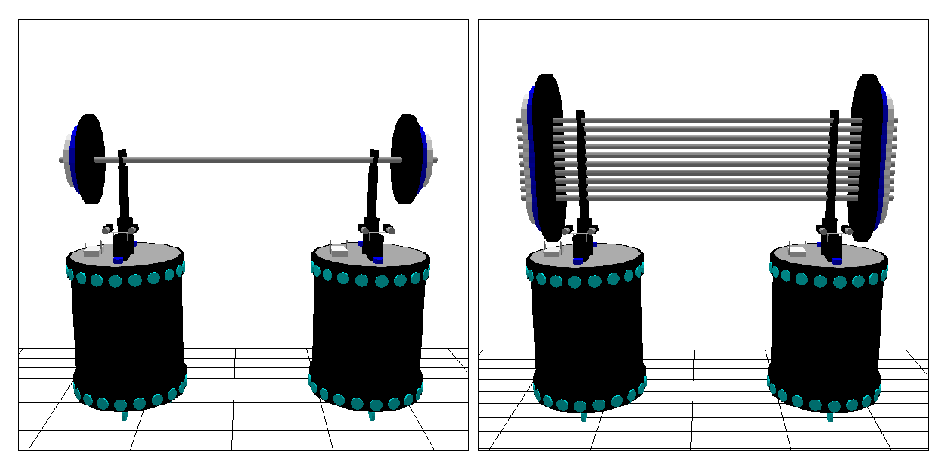
\includegraphics[width=10cm]{FIG/Constraint/halteres.eps}
}
\centerline{
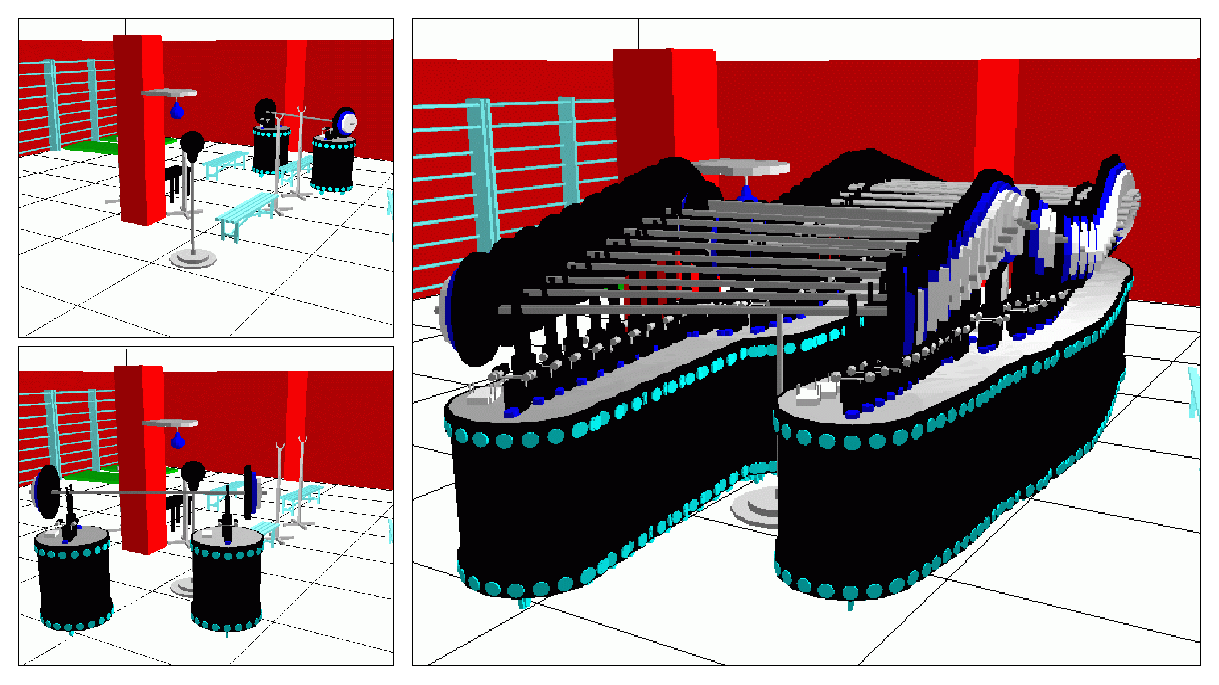
\includegraphics[width=10cm]{FIG/Constraint/halteres2.eps}
}
\caption{\label{fig:halteres} Two holonomic robots cooperating in a
task. The bar with the weighs must stay horizontal, so the hydraulic
bars of the robots must move at the same time.}
\end{figure}


Another example of application of this kinematic constraint would be
the incorporation of natural effects in the simulating model. The
constraint represented in Figure~\ref{fig:dedos} corresponds to the
natural motion of a finger. There is a relationship between the
movement of the phalanges of a hand finger. It could be modeled in a
simple way as a linear relationship.

\begin{figure}[ht!]
%\vspace{15.0mm}
\begin{center}
  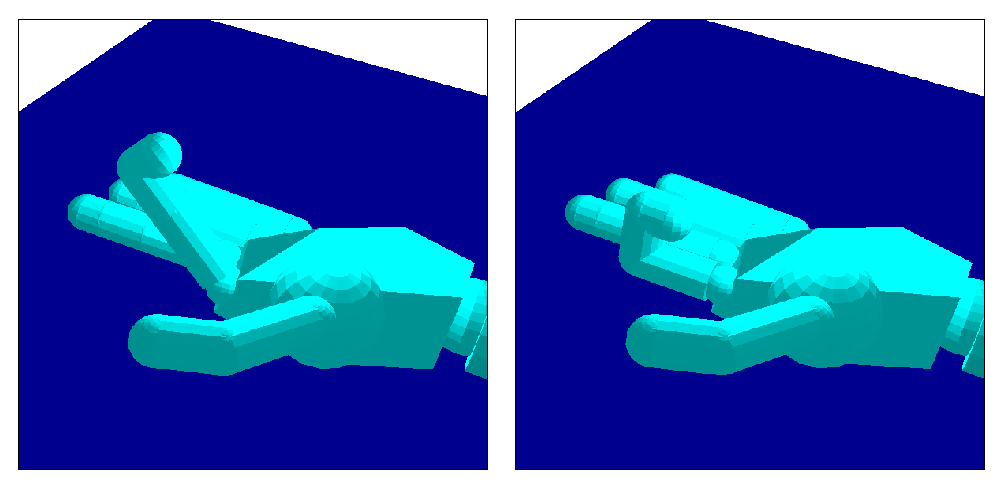
\includegraphics[width=10.0cm]{FIG/Constraint/dedos.eps}
\end{center}
\caption{\label{fig:dedos} Constraint in the movement of a finger. The 
left figure shows an abnormal position for a finger, the right one shows a 
normal situation.}
%\vspace{5.0mm}
\end{figure}


\subsection*{$RRPR$, $4R$ and $3RPR$ linkages}

The $RRPR$, $4R$ nd $3RPR$ linkages are basic planar closed kinematic
chains. Theirs constraint equations are calculated by planar geometry,
likewise theirs motion limits. It must be remarked that {\bf joints
  affected by these constraints must be defined on the same plane}.
Next each one of these linkages will be separately explained.

%\vspace{5.0mm}
\begin{figure}[ht!]
%\vspace{5.0mm}
\begin{center}
\psfrag{teta}[l]{$\theta$} 
\psfrag{chi}[l]{$\psi$}
\psfrag{r}[l]{$r$}
\psfrag{s}[l]{$s$}
\psfrag{g}[l]{$g$}
\psfrag{e}[l]{$e$}
  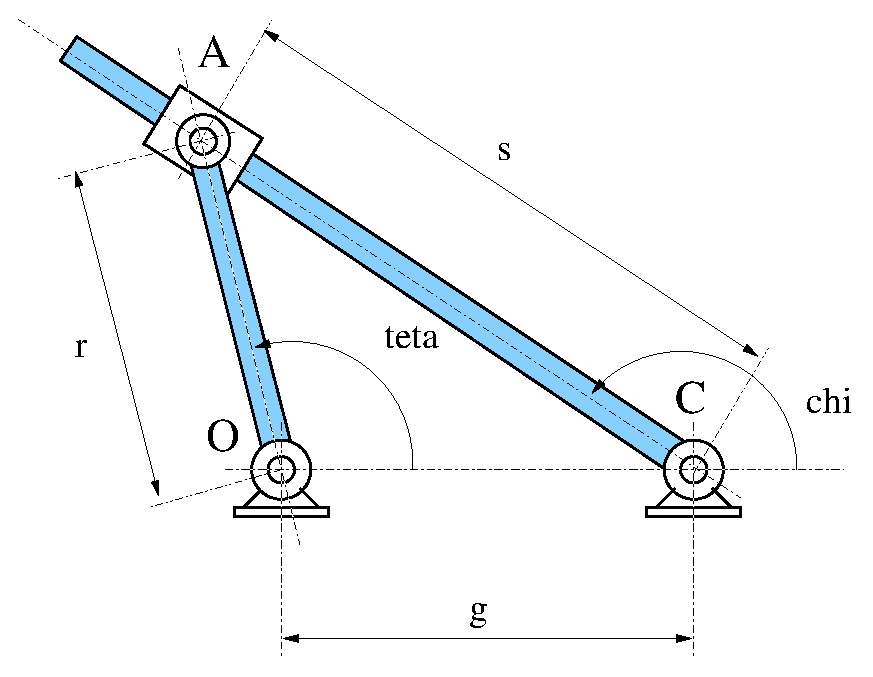
\includegraphics[width=7.0cm]{FIG/Constraint/RRPR2.eps}
\end{center}
\caption{\label{fig:RRPR} The dimensions characterizing an $RRPR$
linkage.}
%\vspace{5.0mm}
\end{figure}


The $RRPR$ linkage is known as a {\em slider-crank} and consist of two
rotating cranks linked by a translating slider. It is a one
degree-of-freedom planar closed chain that is a fundamental machine
element found in everything from automotive engines to door closing
mechanisms.

In the implementation of this constraint in Move3D, the
translation $s$ has been chosen to be the d.o.f. that controls the chain. Therefore,
the joint representing $s$ ($JA$) will be the active joint and the joints
representing $\theta$ ($JO$) and $\psi$ ($JC$) will be the passive
ones. Notice that $JO$ and $JC$ must have the same parent, and $JA$
must be placed in the point corresponding to {\bf A} in the modeling.

\begin{figure}[ht!]
\begin{center}
\psfrag{teta}[l]{$\theta$} 
\psfrag{chi}[l]{$\psi$}
\psfrag{fi}[l]{$\phi$}
\psfrag{a}[l]{$a$}
\psfrag{h}[l]{$h$}
\psfrag{g}[l]{$g$}
\psfrag{b}[l]{$b$}
 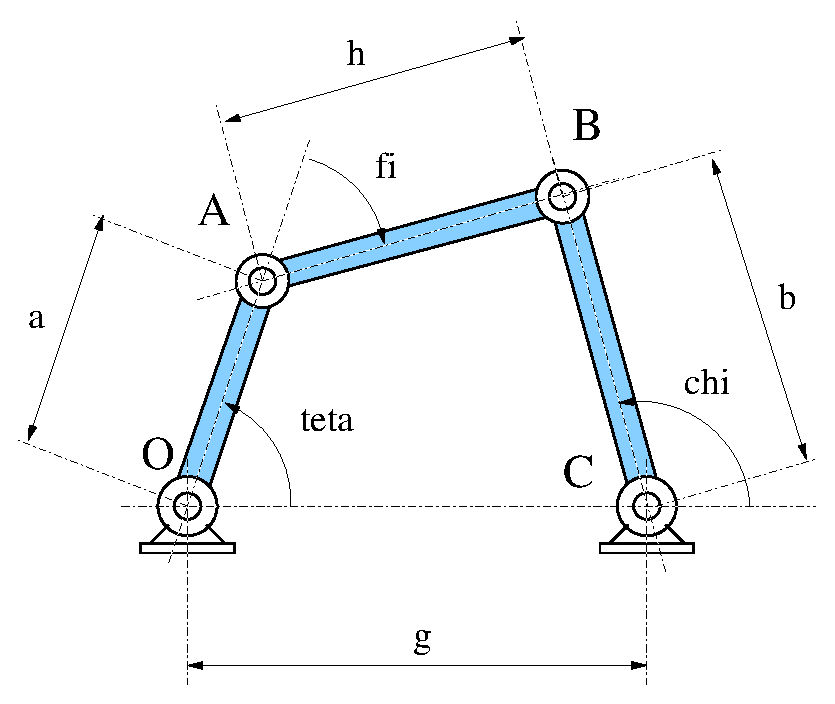
\includegraphics[width=7.0cm]{FIG/Constraint/4R.eps}
\end{center}
\caption{\label{fig:4R} The dimensions characterizing an $4R$ linkage.}
\end{figure}

The $4R$ linkage is a four-rotations planar closed chain. It consist
of an input crank ({\bf OA}), an output crank ({\bf CB}) and a coupler 
({\bf AB}). There is also just one d.o.f. in this fundamental mechanism,
which is the input crank.  

The following remarks must be obeyed for the modeling of this chain:
$JO$ and $JC$ must be defined on the same solid; the coupler must be
defined from the input crank, that is, the chain is cut at {\bf B};
the joint $JB$ can be placed at the end of the output crank or at the
end of the coupler, but this joint is necessary in order to calculate
lengths of the links.

The $3RPR$ linkage can be seen as a $4R$ linkage where the length of
the output crank is variable. It is, therefore, a two d.o.f. planar
closed chain. These two active joints corresponds to the input crank
({\bf OA}) and the translating slider placed at {\bf B} on the output
crank. 

\begin{figure}[ht!]
\begin{center}
\psfrag{teta}[l]{$\theta$} 
\psfrag{chi}[l]{$\psi$}
\psfrag{fi}[l]{$\phi$}
\psfrag{a}[l]{$a$}
\psfrag{h}[l]{$h$}
\psfrag{g}[l]{$g$}
\psfrag{s}[l]{$s$}
 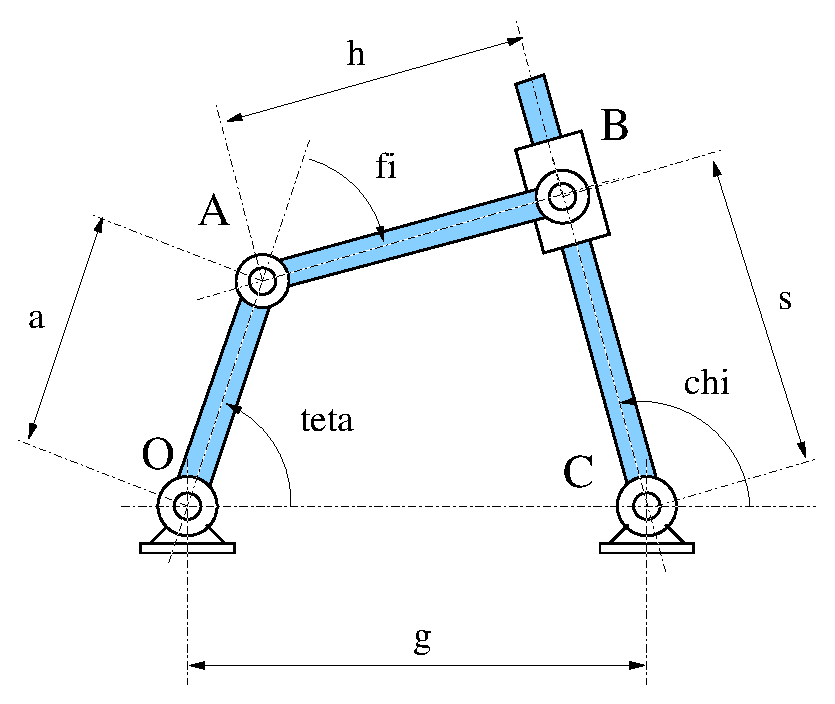
\includegraphics[width=7.0cm]{FIG/Constraint/3RPR.eps}
\end{center}
\caption{\label{fig:3RPR} The dimensions characterizing an $3RPR$ linkage.}
\end{figure}

The remarks for the modeling are similar to the ones made for the
$4R$ linkage, but in this case $JB$ is the translating joint, and it
must be defined from the output crank.

Now, some of the results obtained before the
implementation of these constraints in Move3D will be shown. Figures~\ref{fig:excavator}
represents the model of an hydraulic excavator. The motion of its arm
is controlled by the hydraulic systems, so there are 3 d.o.f.. This
mechanical system contains four closed kinematic chains. Three of them
are the hydraulic systems, and the fourth one is the mechanism for the
motion of the bucket. The hydraulic systems can be modeled as $RRPR$
linkages where the translating crank is the hydraulic bar. The
mechanism of the bucket is a $4R$ linkage. But the third hydraulic
system and the mechanism of the bucket are linked, so we really have
two single closed chains and one double loop closed chain.

\begin{figure}[hb!]
\begin{center}
  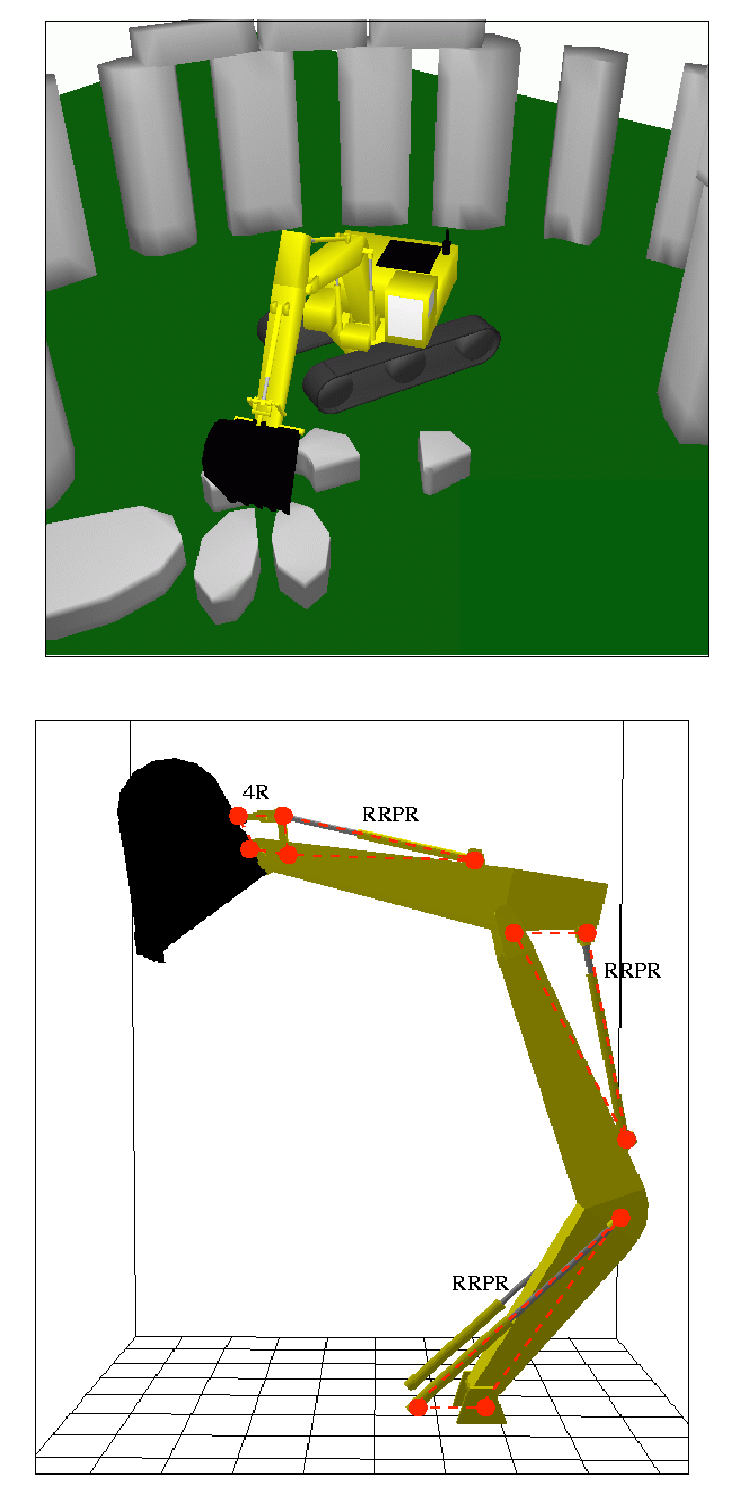
\includegraphics[width=8.1cm]{FIG/Constraint/excavator.eps}
\end{center}
\caption{\label{fig:excavator} Hydraulic excavator. This model
contains two single closed chains and one double loop closed chain. The 
arm, a mechanical system of 19 d.o.f. has been constrained to a system of 3 d.o.f..}
\end{figure}


\begin{figure}[ht!]
\begin{center}
  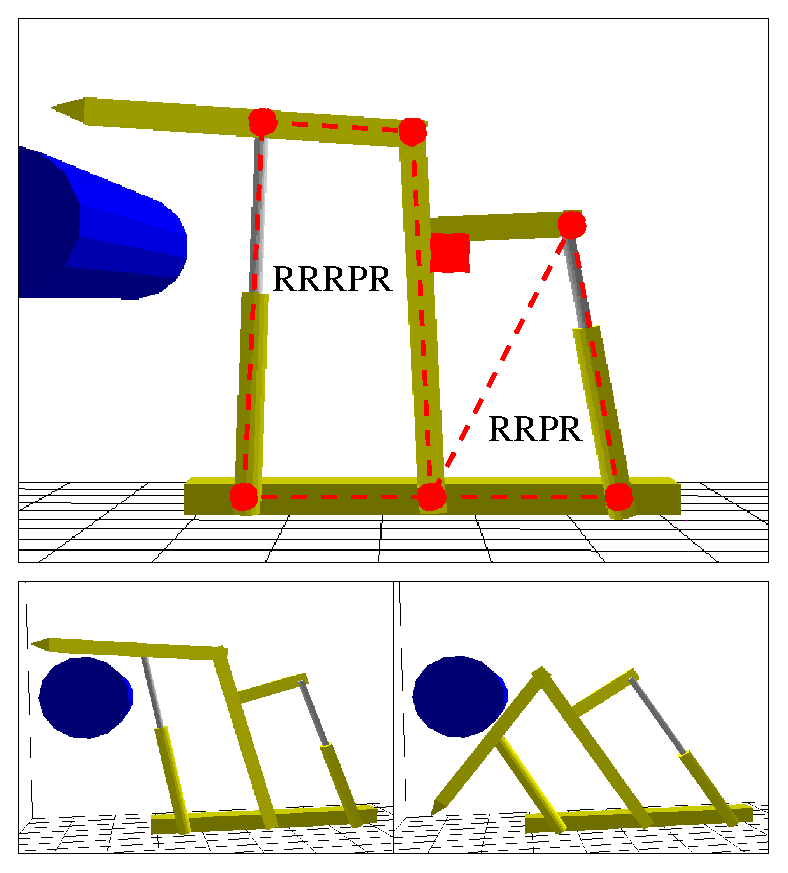
\includegraphics[width=8.0cm]{FIG/Constraint/liegeois.eps}
\end{center}
\caption{\label{fig:liegeois} Manipulator shown in some works of Liegeois.
This two d.o.f. mechanical system consist of a double loop closed chain.} 
\end{figure}

The mechanical system in Figures~\ref{fig:liegeois} is another example
of a double loop closed chain. In this case, the two single chains are 
a $RRPR$ linkage for the rear hydraulic system, and a $3RPR$ linkage
for the front loop.


\subsection*{Contact with ground}

This kinematic constraint represents the case when an object is
required to stay in contact with an obstacle. Particularly, the
implemented constraint corresponds to an object that have to move with
its lowest point sliding on the ground.

The kind of problems which we are mainly interested in are mobile
machines (robots) carrying long objects that have to trail on the
ground. However, the general problem has not been already solved. Just
the last joint of the robot, that is, the joint of the terminal organ
of the robot which grasp the carried object, is going to be
controlled.  This joint must be a revolute joint turning around an
axis perpendicular to the absolute $z$-axis of the scene. This
particular case can be seen as a planar problem.

\begin{figure}[ht!]
\begin{center}
\psfrag{te}[l]{$\theta$} 
\psfrag{li}[l]{$\theta_{JC}$}
\psfrag{de}[l]{$\theta o_{JC}$}
\psfrag{ang}[l]{$\theta_{Object}$}
\psfrag{ant}[l]{$\theta_P$}
\psfrag{d}[l]{$d$}
\psfrag{z_J}[l]{$z_J$} 
\psfrag{z_G}[l]{$z_0$}    
  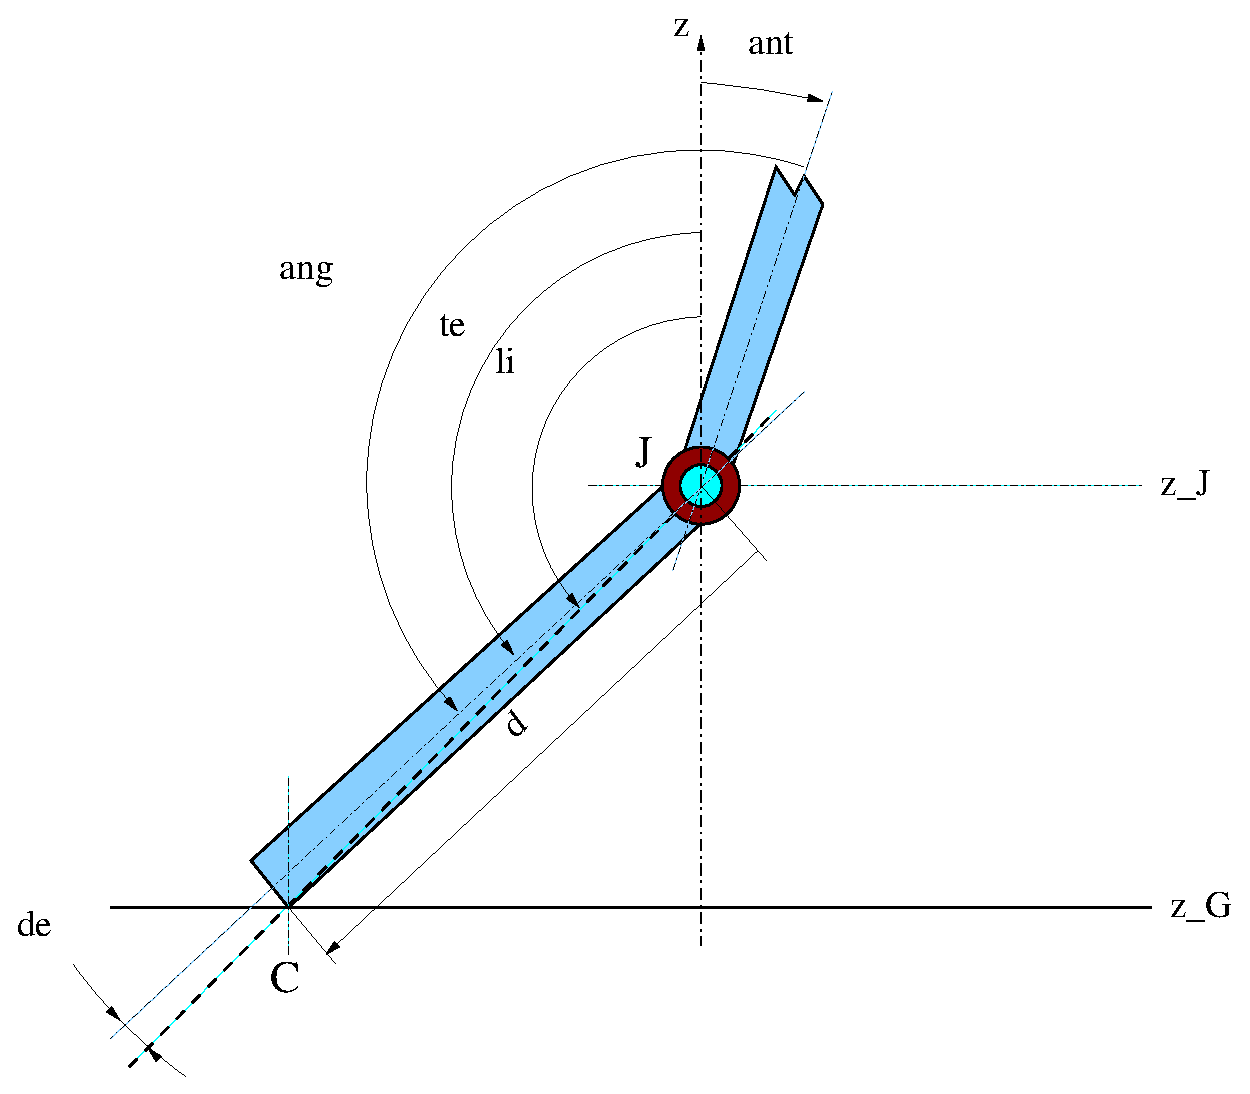
\includegraphics[width=7cm]{FIG/Constraint/ground.eps}
\end{center}
\caption{\label{fig:ground} Variables and references in the analysis.}
\end{figure}

Some remarks for the modeling must be made for this constraint. Let us 
suppose that, for long-shaped objects, the point having to stay
in contact with the ground does not change. In the file containing the
workspace for the path planning with Move3D, the carried object must
be modeled as another body of the robot. Therefore, a joint can be
placed in the point of this `body' that has to slide on the ground.
This joint will be or not a connection with another body, so it will
be not a real joint, but it is necessary to include it in the model.
Let us call it {\bf $J_C$} because it is placed at the point {\bf C}.
It must not be forgotten during the modeling that we are solving a
planar problem. That is to say that the points {\bf J} and {\bf $J_C$}
must be in the same plane, and this plane must be perpendicular to the
rotation axis of the joint at {\bf J}.

\begin{figure}[ht!]
\begin{center}
  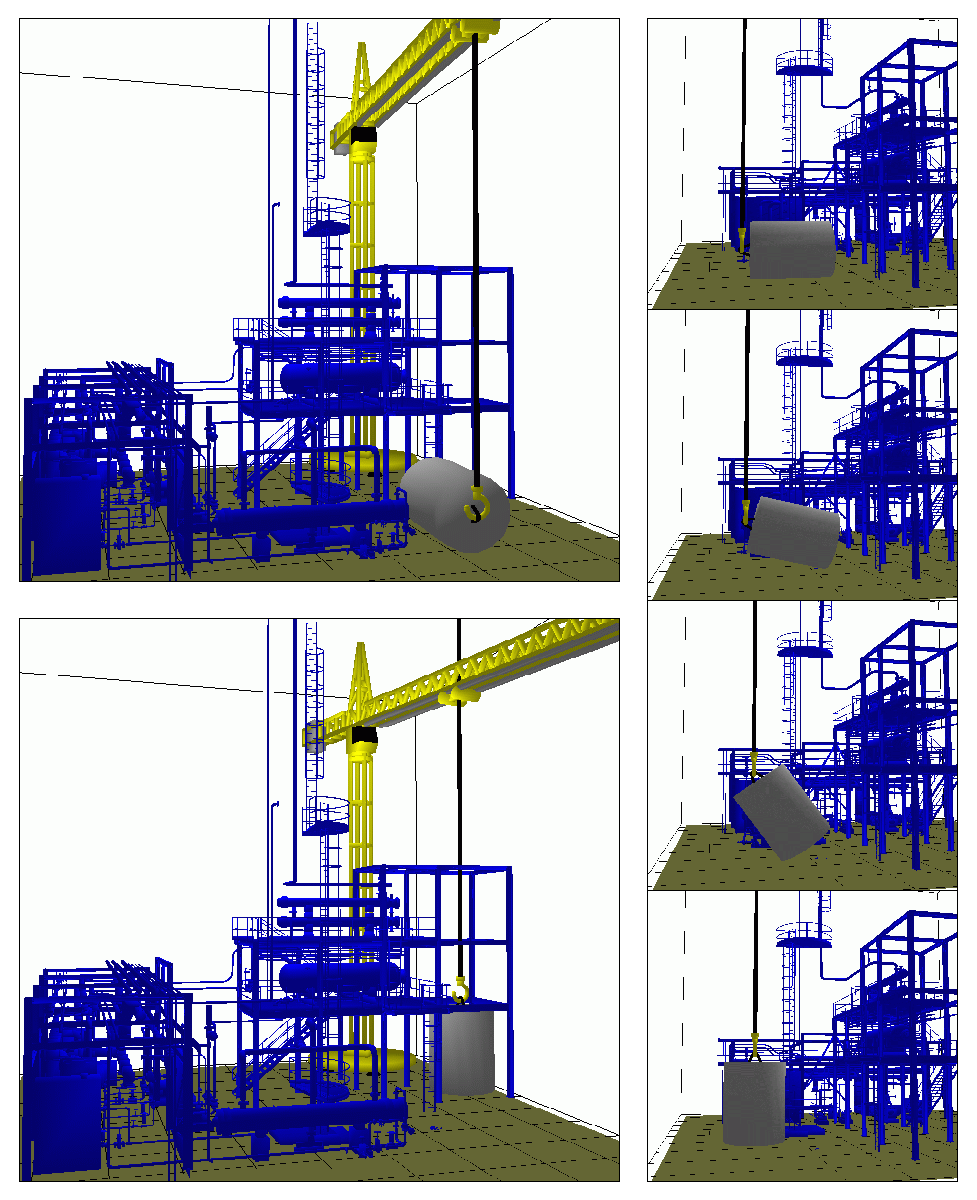
\includegraphics[width=8.0cm]{FIG/Constraint/grue.eps}
\end{center}
\caption{\label{fig:gruaind} A crane has to place a tank into a
metallic structure in an industrial environment. In the initial
configuration, the tank is horizontally placed on the ground. The tank
has to slide on the ground before it reaches the vertical position.}
\end{figure}

Applications of this kind of kinematic constraint are particularly
interesting. For instance, in industrial environments they exist path
planning problems where a moving object must stay in contact with the
ground following physical laws. Figure~\ref{fig:gruaind} shows an
example of one of these problems. The typical example of application,
also usual in the industrial environments, consist in a `robot'
carrying long-shaped objects with a point sliding on the ground. The
example in Figure~\ref{fig:pipe} shows the performance of the planner
handling this kind of kinematic constraint.

\begin{figure}[ht!]
\centerline{
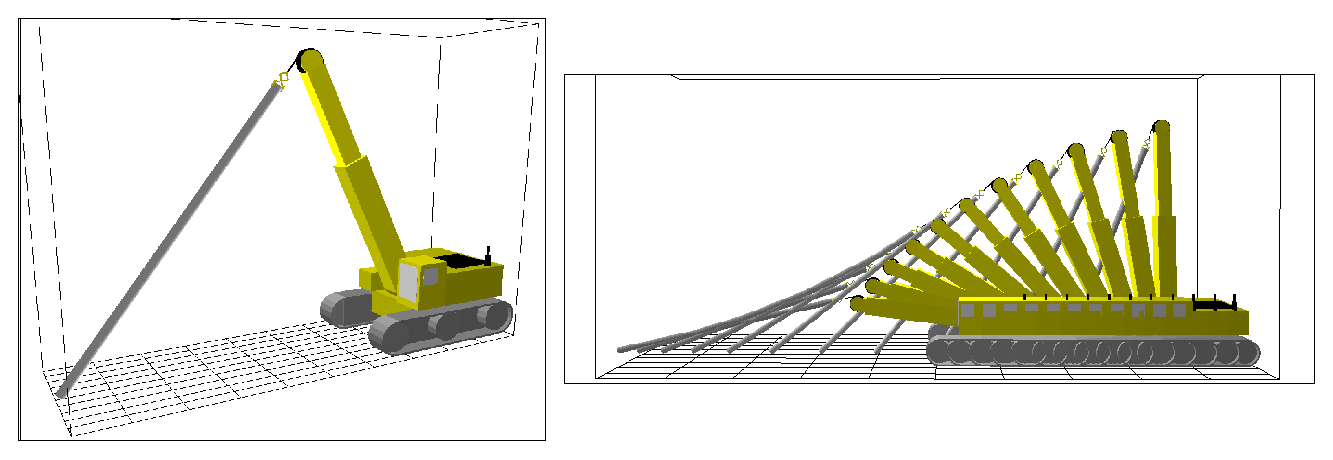
\includegraphics[width=15cm]{FIG/Constraint/pipe12.eps}
}
\caption{\label{fig:pipe} A telescopic handler carries a long
pipe. The lowest extreme of the pipe must stay in contact with the
ground all along the path.}
\end{figure}

\subsection*{Car front wheels}

\begin{figure}[ht!]
\begin{center}
\psfrag{t}[l]{$\theta$} 
\psfrag{O}[l]{O} 
\psfrag{P}[l]{P}    
  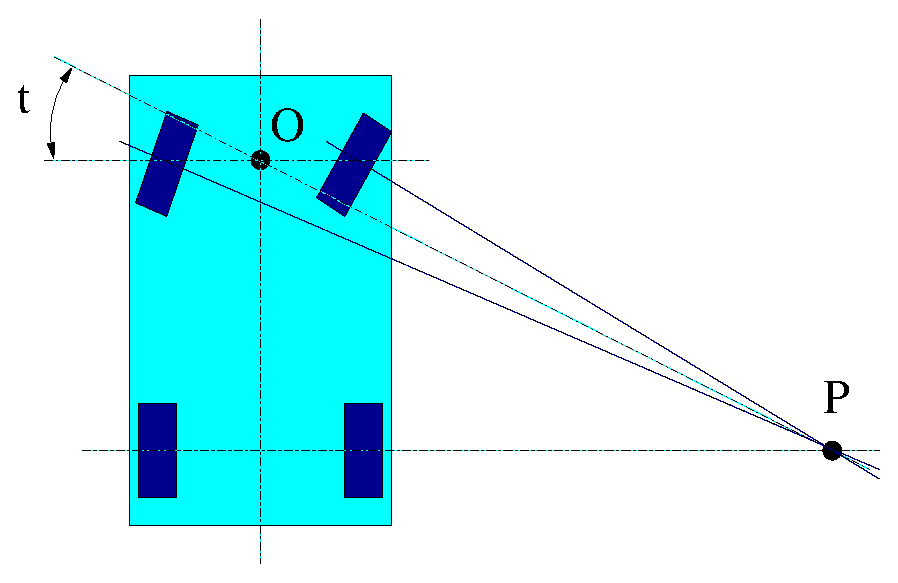
\includegraphics[width=8cm]{FIG/Constraint/carfw.eps}
\end{center}
\caption{\label{fig:carfw} Geometric law for the angles of the car 
  front wheels.}
\end{figure}

This kinematic constraint will be applied to cars. A car can be
modeled as a robot towing a trailer. The steering column of the car is
represented by the robot and the body of the car is represented by the
trailer (see Chapter~\ref{methode-local}). The angle of each
front wheel is then computed as shown on Figure~\ref{fig:carfw}.
That is, the axes of all the wheels (front and rear) must coincide in
a same point {\bf P}.  This point is also the intersection between the
rear wheels axis and the line passing trough the car turning center
(steering column) {\bf O} and having the car turning angle $\theta$.
This point {\bf O} represents the joint between the robot and the
trailer.

Figure~\ref{fig:LegoCar} shows the model of a car
within this constraint has been successfully tried.



\begin{figure}[htb!]
\begin{center}
  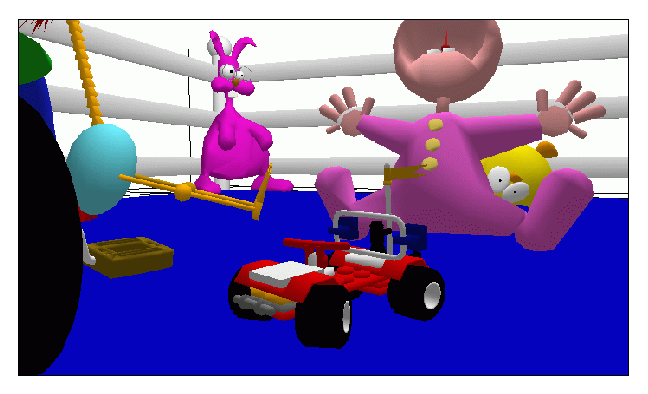
\includegraphics[width=8cm]{FIG/Constraint/LegoCar.eps}
\end{center}
\caption{\label{fig:LegoCar} Three-dimensional model of a LegoCar.}
\end{figure}


\subsection*{Planar closed chain}

A general analytical solution for a planar closed
chain is used in this constraint. It is known that for a n-bar planar mechanism, the number of
d.o.f is n-3. The base of the mechanical system is considered as one
of the bars, then it becomes a (n-1)-bar mechanism with (n-1)-2 d.o.f.
The chosen method to solve this geometrical problem
consist of cutting the loop in two parts. At one side we leave a 2-bar
open chain. At the other side we will have another open chain with the
rest of the elements. The two joints of the first part will be the
passive joints (the two lost d.o.f.), while the joints the other part
remain active. The angles of the passive joints are calculated by
trigonometric laws in order to close the loop.

\begin{figure}[h!]
\begin{center}
\psfrag{a}[l]{$\theta 1$} 
\psfrag{b}[l]{$\theta 2$}
\psfrag{chi}[l]{$\psi$}
\psfrag{fi}[l]{$\phi$}
\psfrag{d}[l]{$d$}
\psfrag{any planar open chain}[l]{any planar open chain}
  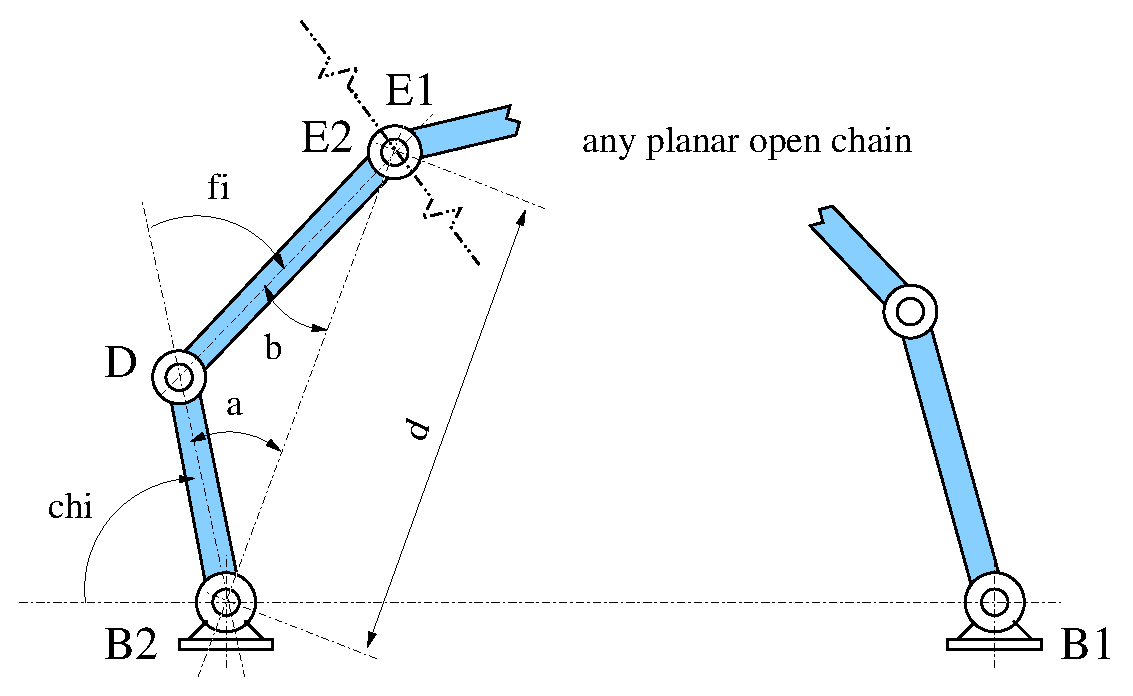
\includegraphics[width=7cm]{FIG/Constraint/plclch.eps}
\end{center}
\caption{\label{fig:plclch} Variables and references in the analysis.}
\end{figure}

Figure~\ref{fig:plclch} represents the way how a mechanical system 
containing this kinematic constraint must be modeled. Joints ({\bf E1}
and {\bf E2}) must be placed at the end of each open chain.

Figure~\ref{fig:cad8pas} shows the performance of Move3D solving a 
path planning problem for a 8-bar closed chain.

\begin{figure}[h!]
\begin{center}
  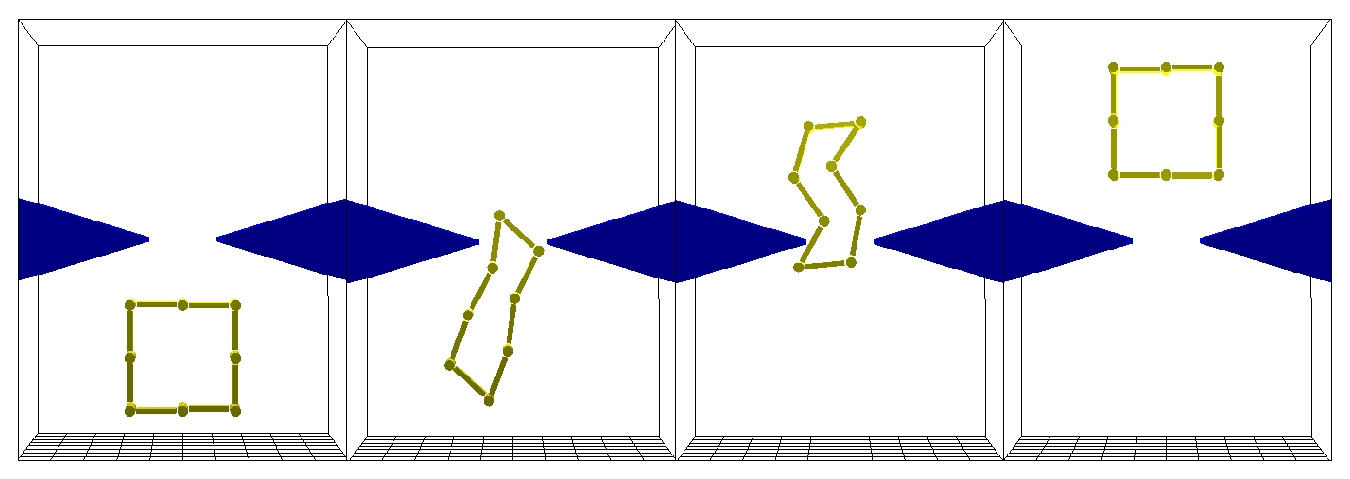
\includegraphics[width=10cm]{FIG/Constraint/cad8pas.eps}
\end{center}
\caption{\label{fig:cad8pas} Some sequences of the solution given
  by Move3D for a 8-bar closed chain that has to find a path trough a
  narrow passage.}
\end{figure}

\section{How to use them}

Kinematic constraints can be set in the mechanical system in two ways: 
they can be directly set in the model input file ({\tt .p3d}), or they can
be set once Move3D is running. Next, this two
possibilities are explained.

\subsection*{Kinematic constraints in the {\tt .p3d} file}

Constraints can be introduced in the mechanical system by adding command 
lines at the end of the model input file. These command lines have the 
following structure: 

\hspace{-4.0mm}
{\tt p3d\_constraint \footnotesize cntrt\_name npasjnts \{pj1...pjn\} nactjnts
  \{aj1...ajn\} nc \{c1...cn\} no \{o1...on\}} \index{p3d\_constraint} \\

where:
\begin{tabbing}
>>>\=>>>>>>>>>>>>> \= \kill
\> - {\tt cntrt\_name} \>: is the name of the kinematic constraint to 
  be set.\\
\> - {\tt npasjnts}   \>: is the number of passive joints.\\
\> - {\tt \{pj1...pjn\}}\>: are the indexes corresponding to each one of 
  the passive joints.\\
\> - {\tt nactjnts}   \>: is the number of active joints.\\
\> - {\tt \{aj1...ajn\}}\>: are the indexes corresponding to each one of 
  the active joints.\\
\> - {\tt nc}         \>: is the number of (real) constant parameters.\\
\> - {\tt \{c1...cn\}}  \>: are the constant parameters of the
  constraint.\\
\> - {\tt no}          \>: is the number of other (integer) constant parameters.\\
\> - {\tt \{o1...on\}}   \>: are integer constant parameters of the
  constraint.\\
\end{tabbing}

  
For each one of the kinematic constraints explained in
the last section, the parameters of this command line are as follows
(see figures in last section for the references of points and joints):

\begin{tabbing}
>\=>>\=>>>>>>>>>>>>\=>>>\= \kill
\>{\normalsize \bf Linear relationship between two d.o.f.} \\
\>\>\\
\>\>{\bf \tt cntrt\_name} \>: {\tt p3d\_lin\_rel\_dofs}\\
\>\>{\bf \tt npasjnts} \>: 1\\
\>\>{\bf \tt pj1} \>: index of the joint to be controlled ($JA$)\\
\>\>{\bf \tt nactjnts} \>: 1\\
\>\>{\bf \tt aj1} \>: index of the joint that controls $JA$ ($JB$)\\
\>\>{\bf \tt nc} \>: 2\\
\>\>{\bf \tt c1} \>: linear relationship coefficient ($K$)\\
\>\>{\bf \tt c2} \>: offset ($C$)\\
\>\>{\bf \tt no} \>: 0\\
\>\>\\
\>{\normalsize \bf $RRPR$ linkage} \\
\>\>\\
\>\>{\bf \tt cntrt\_name} \>: {\tt p3d\_RRPRlnk}\\
\>\>{\bf \tt npasjnts} \>: 2\\
\>\>{\bf \tt pj1} \>: index of the joint corresponding to {\bf O}\\
\>\>{\bf \tt pj2} \>: index of the joint corresponding to {\bf C}\\
\>\>{\bf \tt nactjnts} \>: 1\\
\>\>{\bf \tt aj1} \>: index of the translating joint, placed at {\bf A}\\
\>\>{\bf \tt nc} \>: 0\\
\>\>{\bf \tt no} \>: 0\\
\>\>\\
\>{\normalsize \bf $4R$ linkage} \\
\>\>\\
\>\>{\bf \tt cntrt\_name} \>: {\tt p3d\_4Rlnk}\\
\>\>{\bf \tt npasjnts} \>: 3\\
\>\>{\bf \tt pj1} \>: index of the joint corresponding to {\bf A}\\
\>\>{\bf \tt pj2} \>: index of the joint corresponding to {\bf B}\\
\>\>{\bf \tt pj3} \>: index of the joint corresponding to {\bf C}\\
\>\>{\bf \tt nactjnts} \>: 1\\
\>\>{\bf \tt aj1} \>: index of the joint corresponding to {\bf O}\\
\>\>{\bf \tt nc} \>: 0\\
\>\>{\bf \tt no} \>: 0\\
\>\>\\
\>{\normalsize \bf $3RPR$ linkage} \\
\>\>\\
\>\>{\bf \tt cntrt\_name} \>: {\tt p3d\_3RPRlnk}\\
\>\>{\bf \tt npasjnts} \>: 2\\
\>\>{\bf \tt pj1} \>: index of the joint corresponding to {\bf A}\\
\>\>{\bf \tt pj2} \>: index of the joint corresponding to {\bf C}\\
\>\>{\bf \tt nactjnts} \>: 2\\
\>\>{\bf \tt aj1} \>: index of the joint corresponding to {\bf O}\\
\>\>{\bf \tt aj2} \>: index of the translating joint, placed at {\bf B}\\
\>\>{\bf \tt nc} \>: 0\\
\>\>{\bf \tt no} \>: 0\\
\>\>\\
\>{\normalsize \bf Contact with ground} \\
\>\>\\
\>\>{\bf \tt cntrt\_name} \>: {\tt p3d\_jnt\_on\_ground}\\
\>\>{\bf \tt npasjnts} \>: 1\\
\>\>{\bf \tt pj1} \>: index of the joint sliding on the ground ($J_C$)\\
\>\>{\bf \tt nactjnts} \>: 0\\
\>\>{\bf \tt nc} \>: 2\\
\>\>{\bf \tt c1} \>: height ($z$) of the ground\\
\>\>{\bf \tt c2} \>: offset with relation to the horizontal plane
when the body is hanging\\
\>\>{\bf \tt no} \>: 3  (for these variables: 0 == OFF, 1 == ON)\\
\>\>{\bf \tt o1} \>: $J_C$ turns in the negative direction\\
\>\>{\bf \tt o2} \>: $J_C$ changes the turning direction depending on
the position of the rest\\\>\>\>\> of bodies of the robot\\
\>\>{\bf \tt o3} \>: the carried body must stay on the ground (it can
not be hung)\\
\>\>\\
\>{\normalsize \bf Car front wheels} \\
\>\>\\
\>\>{\bf \tt cntrt\_name} \>: {\tt p3d\_car\_front\_wheels}\\
\>\>{\bf \tt npasjnts} \>: 2\\
\>\>{\bf \tt pj1} \>: index of the joint corresponding to the right wheel\\
\>\>{\bf \tt pj2} \>: index of the joint corresponding to the left wheel\\
\>\>{\bf \tt nactjnts} \>: 1\\
\>\>{\bf \tt aj1} \>: index of the joint corresponding to the steering
column {\bf O}\\
\>\>{\bf \tt nc} \>: 2\\
\>\>{\bf \tt c1} \>: distance between front and rear wheels axes\\
\>\>{\bf \tt c2} \>: distance between front wheels\\
\>\>{\bf \tt no} \>: 0\\
\>\>\\
\>{\normalsize \bf Planar closed chain} \\
\>\>\\
\>\>{\bf \tt cntrt\_name} \>: {\tt p3d\_planar\_closed\_chain}\\
\>\>{\bf \tt npasjnts} \>: 2\\
\>\>{\bf \tt pj1} \>: index of the last joint of the controllable (active) half-chain {\bf E1}\\
\>\>{\bf \tt pj2} \>: index of the last joint of the non-controllable (passive) half-chain {\bf E2}\\
\>\>{\bf \tt nactjnts} \>: 1\\
\>\>{\bf \tt aj1} \>: index of the first joint of the controllable half-chain {\bf B1}\\
\>\>{\bf \tt nc} \>: 0\\
\>\>{\bf \tt no} \>: 0\\
\end{tabbing}


\subsection*{Setting and modification of constraints while Move3D is running}

The access to the kinematic constraints, while Move3D is running, is
got from the so called button in the robot control window. This button 
generates the {\em kinematic constraints window} (see
Figure~\ref{fig:kcwin}). This window allows the user to manage
three operations:

\begin{figure}[b!]
\begin{center}
  \includegraphics[width=7.9cm]{FIG/Constraint/kcwin.ps}
\end{center}
\caption{\label{fig:kcwin} Kinematic constraints window. In this
  case, the list of constraints corresponds to the model of the
  excavator arm (see Figure~\ref{fig:excavator}).}
\end{figure}

\begin{itemize}
\item {\bf Activation and deactivation of constraints :} \\
Buttons placed at the left on the kinematic constraints window allow
to activate (pushed) or deactivate (released) any of the already set
constraints. It is important to remark at this point that two kinematic
constraints having the same passive joints can not be active at the
same time.
\item {\bf Modification of some of the parameters of constraints:} \\
A window containing the parameters of each one of the listed constrains 
appears by pushing its corresponding button at the right of the
kinematic constraints window. In this window, the user can modify
some of the parameters of the constraint. Parameters related to joints 
indexes are forbidden to be changed. Upper part of Figure~\ref{fig:jogwins}
represents an example of these windows.
\item {\bf Setting of new constraints:} \\
Kinematic constraints non-included in the model input file can be
introduced in the mechanical system during the running of Move3D. The
{\em kinematic constraints setting window} appears by pushing the button
``NEW'' on the kinematic constraints window. This window contains the 
list of the kinematic constraints types treated in Move3D. Buttons
placed at the right on this window generate the setting windows of
each one of them. The parameters appearing in these setting windows
have been explained in Section ``Treated constraints''. New
constraints containing wrong parameters will not be set, and an error
message will be displayed. Bottom part of Figure~\ref{fig:jogwins} illustrates
the process for a new constraint setting.
\end{itemize}

\begin{figure}[h!]
\begin{center}
  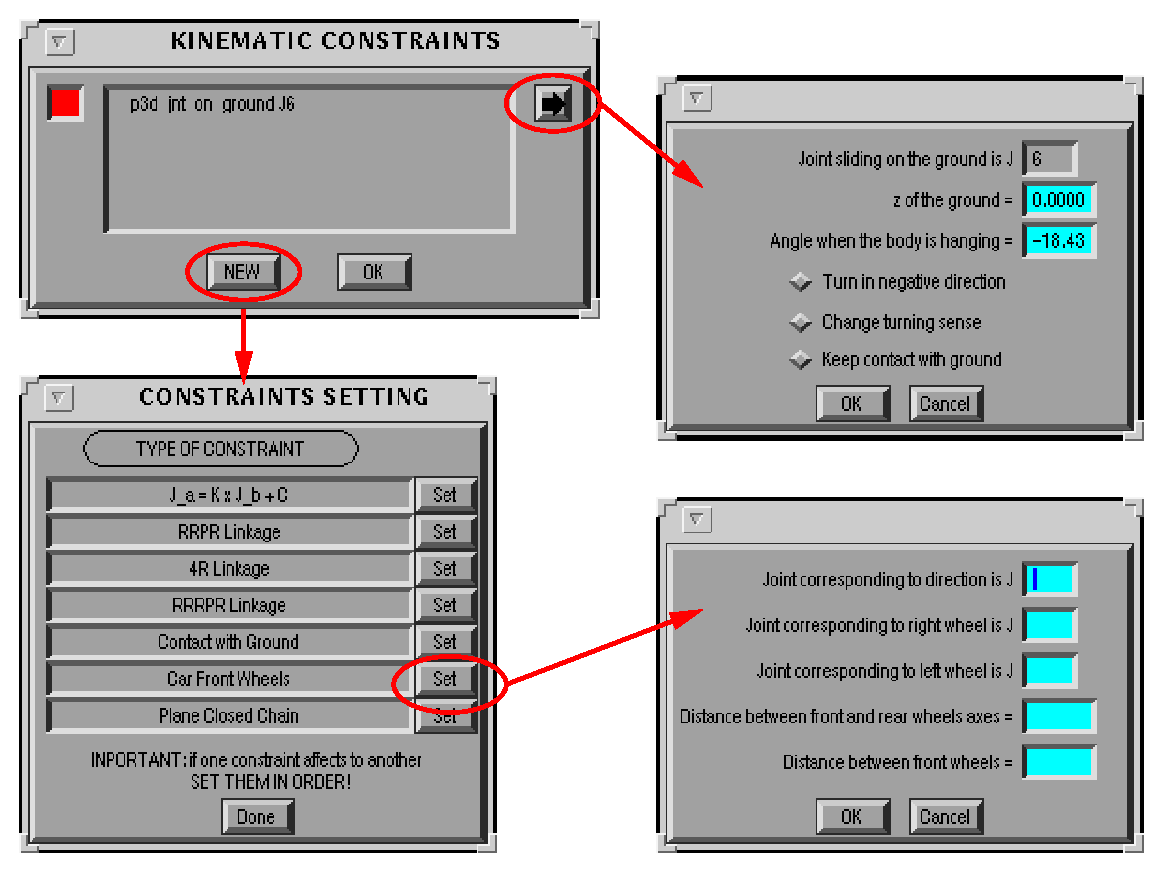
\includegraphics[width=14.0cm]{FIG/Constraint/jogwins.eps}
\end{center}
\caption{\label{fig:jogwins} Kinematic constraints window, kinematic
  constraints setting window, window containing the parameters of a
  constraint and setting window of a constraint.}
\end{figure}
 

\section{Implementation}

When a kinematic constraint is set, its data structure is
generated. This data structure contains all the necessary information
for the treatment of the constraint. The representation in C language
of this structure is:
{\tt
\begin{tabbing}
>>>>>>>>>>>>\=>>\=>>>>>>>>>>>> \= \kill
\>typedef struct cntrt \{ \\ 
\>\>  int       \> num;\\
\>\>  char      \> namecntrt[40];\\
\>\>  int       \> active;\\
\>\>  int       \> (*fct\_cntrt)(struct cntrt *ct);\\
\>\>  int       \> nactjnts, npasjnts;\\
\>\>  int       \> ndval, nival;\\
\>\>  int       \> actjnts[MAX\_ARGU\_CNTRT];\\
\>\>  int       \> actjnt\_state[MAX\_ARGU\_CNTRT];\\
\>\>  int       \> pasjnts[MAX\_ARGU\_CNTRT];\\
\>\>  int       \> argu\_i[MAX\_ARGU\_CNTRT];\\
\>\>  double    \> argu\_d[MAX\_ARGU\_CNTRT];\\
\>\>  int       \> col\_pairs[2][MAX\_ARGU\_CNTRT];\\
\>\>  struct cntrt \> *next\_cntrt;\\
\>\>  struct cntrt \> *prev\_cntrt;\\
\>\>  int       \> enchained\_J[MAX\_ARGU\_CNTRT];\\
\>\>  int       \> nenchained;\\
\>\>  struct cntrt \> **enchained;\\
\>\} p3d\_cntrt,*pp3d\_cntrt; \\
\end{tabbing}
}

Some of the members of this data structure have been already
named, and theirs values are directly given by the user. The rest
of them are automatically calculated in the setting function of each
constraint. In order to  allow a further comprehension about how the
implementation of the kinematic constraints is made, these variables
will be briefly explained next.
\begin{itemize}
\item[$-$] The data structure of each robot in the workspace of Move3D contains 
an array of pointers to the data structures of its kinematic
constraints. {\bf \tt num} represents the index of a constraint in this
list.
\item[$-$] {\bf \tt name} contains the name of the constraint.
\item[$-$] {\bf \tt active} is a flag to indicate the state of the constraint
 (activated/deactivated).
\item[$-$] {\bf \tt fct\_cntrt} is a pointer to the function
containing the equations to solve this constraint type.
\item[$-$] {\bf \tt nactjnts} and {\bf \tt npasjnts} are respectively the number
  of active and passive joints of the constraint.
\item[$-$] {\bf \tt ndval} and {\bf \tt nival} are respectively the
  number of real and integer constant parameters of the constraint
  that are given by the user.
\item[$-$] {\bf \tt actjnts} and {\bf \tt pasjnts} are arrays containing the indexes of 
the active and passive joints in this constraint.
\item[$-$] {\bf \tt actjnt\_state} is an array of flags for the active joints of
the constraint. A flag set to $0$ means that the corresponding joints
is involved in a previously defined constraint.
\item[$-$] {\bf \tt argu\_i} and {\bf \tt argu\_d} contain respectively integer and
real constant parameters of the kinematic constraint. Some of these
parameters are the ones introduced by the user. The rest are
automatically calculated. The kind of these calculated constants are, for
example: flags, distances between joints or values to refer angles.
\item[$-$] {\bf \tt col\_pairs} is used to stock information for the 
  deactivation of pairs of bodies for the collision checking.
\item[$-$] {\bf \tt next\_cntrt} and {\bf \tt prev\_cntrt} are
  pointers to the next and preceding constraints in the above
  mentioned list.
\item[$-$] {\bf \tt enchained\_J}, {\bf \tt nenchained} and {\bf \tt enchained} are used for 
  the treatment of {\em multi-constraints}. This concept will be
  explained later.
\end{itemize}


Two special remarks can be made at this point. These remarks ascribe
collision checking and multi-constraints.

Pairs of consecutive bodies
of a robot are deactivated for the collision checking in Move3D. This
same rule must be followed, for instance, when a kinematic chain is
closed. In this case, collisions between the pair of bodies closing the
chain have not to be tested. Deactivation of pairs affected by
kinematic constraints is carried out form the information stocked in the 
matrix {\tt col\_pairs}.

A special treatment of kinematic constraints have to be made when they
are {\em enchained}. A multi-constraint can be defined as several
kinematic constraints where active joints of some of them are passive
joints for some others. Two kinematic constraints obeying this property are
told to be enchained. An example of enchained constraints are
multi-loop closed chains. Notice that {\bf constraints to
  be enchained must be set in order}, that is to say: if an active
joint in a constraint is a passive joint in another one, this last
constraint must be defined first.


\section{New kinematic constraints}

The way how the treatment of kinematic constraints has been
implemented in Move3D allows that new constraints will be easily added
to the software. The work to do for this purpose have to be developed in the files {\bf
  FORMconstraints.c} and {\bf p3d\_constraints.c}. The first one
contains all the functions related with interface windows. If a new
constraint is wanted to be added, its related functions in this file
will be easily programmed by following the same procedure that for the
rest of constraints. The functions to be added in file {\bf
  p3d\_constraints.c} are the function for the setting of the new
constraint and the one containing its geometric constraint
equation(s). The calculations of the parameters related with the
constraint that are not going to change during the current running of Move3D
have to be made just once. These operations must be placed in the
setting function. The rest of the operations have to be made each time 
that the function with the constraint equation(s) is called, so they
must be placed inside it.



\clearemptydoublepage
\def\hsp{\hspace*{1cm}}

\chapter{Steering methods and local paths}
\label{methode-local}
\def\CS{{\cal C}}

Local path is the element that encodes elementary motion in Move3D:
trajectories are concatenations of local paths, edges of roadmaps
contain local paths. A local path for a given robot is produced by a
local method. In this chapter, we first give a definition of what we
mean by local path. Then we show how different types of local paths
can be handled by Move3D. Finally, we describe the different steering
methods implemented within the software.

\section{Definition of local path and steering method}

\paragraph{Definition and parameterizations of local path.}
A {\em local path} for a robot $r$ is a continuous curve in the
configuration space of the robot and defined over an interval $[0,U]$:
$$
\begin{array}{lcll}
lp: & [0,U] & \rightarrow & \CS \\
    & u &\rightarrow & lp(u)
\end{array}
$$
In the rest of this chapter, $u$ is called the default parameter (or
parameter) of the local path $lp$ and $U$ the parameter range of $lp$.

 The curve can also be parameterized by length (or
  by pseudo-length), 

In addition to the default parameterization, a length parameterization
can be defined. This parameterization has to be defined by the
developper.  The length parameterization is mainly used for optimizing
trajectories.  The optimizing function picks random configurations
over a list of successive local paths. The length parameterization
ensures us that longer local paths are more likely to be chosen than
smaller ones. The length parameterization can be the same as the
default parameterization u.

The length parameter is defined from the default parameter $u$ by an
increasing function $d$ from $[0,U]$ to an interval $[0,L]$. $L=d(U)$
is called the length of the local path. It does not necessarily represent 
a real length. 

\paragraph{Steering method.}
A steering method is a function that maps, to a pair of configurations, a
local path between these configurations. The simplest steering method is the 
linear one. It connects the two configurations by a  straight line in the
space of configuration parameters.
Some robots are subjected to kinematic constraints such as rolling
without slipping for wheeled mobile robots or moving only one degree
of freedom at a time for a rolling bridge. These kinematic constraints
are not specified in the description of the mechanical system. They
are taken into account by the local method. For instance Reeds and Shepp 
steering method builds curves composed of straight lines and arc of circles
for a carlike robot.

\section{Representation of a local path}
\label{sec:representation}

Local paths are encoded by the data-structure {\tt
  p3d\_localpath}\index{Data structures!p3d\_localpath}

A local path is encoded by a variable of type {\tt p3d\_localpath}. This
structure contains 3 types of fields:
\begin{itemize}
\item data generic to any local path,
\item a pointer to data specific to the type of local path
\item pointers to functions specific to the type of local path.
\end{itemize}

The structure {\tt p3d\_localpath} is like an abstract class in an
object-oriented langage. The specific functions are methods associated
to each derived class (each type of local path).

We enumerate now the main fields of the structure {p3d\_localpath}.

\subsubsection*{data generic to any local path.}
\begin{itemize}
\item {\tt type\_lp}: type of local path (linear, reeds and shepp,...).
\item {\tt range\_param}: parameter range of the local path.
\item {\tt length\_lp}: range of the length parameterization.
\end{itemize}

\subsubsection*{specific methods associated to a local path}
\begin{itemize}
\item {\tt length}: computes the length of the local path.
\item {\tt copy}: copies the local path.
\item {\tt extract}: extracts from a given local path the part included between two values of the length parameter of the local path.
\item {\tt destroy}: destroyes the local path.
\item {\tt config\_at\_distance}: computes the configuration at a given
  distance along the local path.
\item {\tt config\_at\_param}: computes the configuration at a given
  parameter along the local path.
\item {\tt stay\_within\_dist}: given the distance of each body of the
  robot to the obstacles, and a position on a local path, this
  function computes an interval of default parameter that ensures the
  user that each body does not move by more than its specified
  distance when the parameter stays in this interval.
\item {\tt cost}: computes the cost of a local path. This cost is used
  in $A^{*}$ procedure to find the best path in the roadmap and during
  optimization to replace a part of a path by a new local path if this
  latter has lower cost.
\item {\tt simplify}: This function does nothing for most local
  paths. given two successive local paths. When two Reeds and Shepp
  local paths are connected, the end of the first one may overlap the
  beginning of the second one. This function detects this kind of
  situation and removes common parts.
\end{itemize}

Data specific to each type of local path are detailled in the
following section.

\section{Local methods implemented within Move3D}

In this section, we describe the various local methods currently supported 
by Move3D. For each of them, we specify the default and length parameterization
used and the data-structures involved.

\subsection{Linear local method}
\label{subsec:linear}

This local method is the simplest one. It connects two configurations
by a straight line in the joint parameter space. If a configuration
parameter represents the rotation angle of a joint without bounds,
along a linear path, this parameter follows the shortest arc between
its initial and final values.

\begin{figure}[ht]
\centerline{\psfig{figure=FIG/localseg.ps, width=6cm}}
\caption{Example of linear local path}
\label{fig:linear-local}
\end{figure}

\subsubsection*{parameterization}

For this type of local path the default and length parameterizations
are the same. Given two configurations, $q_0=(x_0,y_0,z_0,\theta_0,
\phi^{1}_{0},...,\phi^{n}_{0})$ and $q_1=(x_1,y_1,z_1,\theta_1,
\phi^{1}_{1},...,\phi^{n}_{1})$ where the $\phi^i$'s represent the values 
of each joint, we define a distance as follows:
$$
d_{lin}(q_0,q_1) = \sqrt{(x_1-x_0)^2 + (y_1-y_0)^2 + (z_1-z_0)^2 + d_{S^1}(\theta_1-\theta_0)^2 + \sum_{i=1}^{n} d_i(\phi^i_0,\phi^i_1)^2}
$$
where $d_{S^1}$ is the arc length distance over the unit circle, 
\begin{itemize}
\item $d_i(\phi^i_0,\phi^i_1) = |\phi^i_1-\phi^i_0|$ if joint $i$ is a
  translation joint,
  
\item $d_i(\phi^i_0,\phi^i_1) = dist\,|\phi^i_1-\phi^i_0|$ where
  $dist$ is the maximal distance between the points of body $i$ and
  the axis of joint $i$, if this latter is a rotation joint with
  bounds.

\item $d_i(\phi^i_0,\phi^i_1) = dist\, d_{S^1}(\phi^i_0,\phi^i_1)$ if
  joint $i$ is a rotation joint without bounds (i.e. that can rotate
  freely about its axis).
\end{itemize}
The factor $dist$ in front of angular distances makes the linear
distance over the configuration space homogeneous to a length.

\subsubsection*{Data-structure}

Data relative to a linear local path are stored in the following
structure:
\index{Data structures!struct lin\_data}
\index{Data structures!p3d\_lin\_data}
\begin{tabular}{l}{\tt 
struct lin\_data} $\{$ \\
\hsp {\tt configPt q\_init;} \\
\hsp {\tt configPt q\_end;} \\
$\}$ {\tt p3d\_lin\_data, *pp3d\_lin\_data;}\\
\end{tabular}

\noindent
where {\tt q\_init} and {\tt q\_end} are the initial and final
configurations of the local path.

\subsection{Reeds and Shepp + Linear local method}

This local method connects two configurations by Reeds and Shepp
curves in the plane $(x,y)$ for the platform of the robot and linear
curves for the other joints: given two configurations, 
$q_0=(x_0,y_0,z_0,\theta_0, \phi^{1}_{0},...,\phi^{n}_{0})$ and 
$q_1=(x_1,y_1,z_1,\theta_1,\phi^{1}_{1},...,\phi^{n}_{1})$,
$(x_0,y_0,\theta_0)$ and $(x_1,y_1,\theta_1)$ are connected by a
Reeds and Shepp curve of length
$l_{RS}(q_0,q_1)$. $(z_0,\phi^{1}_{0},...,\phi^{n}_{0})$ and
$(z_1,\phi^{1}_{1},...,\phi^{n}_{1})$ are connected
using the linear strategy described in the previous section.

\begin{figure}[ht]
\centerline{\psfig{figure=FIG/RS.ps, width=6cm}}
\caption{Example of Reeds and Shepp + linear local path}
\label{fig:RS-local}
\end{figure}

\subsubsection*{Parameterization}

\paragraph{Default parameterization:} the default parameterization is
the arc-length distance along Reeds and Shepp curve. Thus, the
parameter range is $l_{RS}(q_0,q_1)$.

\paragraph{Length parameterization:} the distance between
configurations $q_0$ and $q_1$ is defined as follows:
$$
d_{RS-lin}(q_0,q_1) = l_{RS}(q_0,q_1) + \sqrt{\sum_{i=1}^{n} d_i(\phi^i_0,\phi^i_1)^2}
$$
where distances $d_i$ are defined as in the previous section. Notice
that the coordinate $z$ does not appear in this distance.

\subsubsection*{Data-structure}

Data relative to a Reeds and Shepp + linear local path are stored in
a list of the following structure:

\index{Data structures!struct rs\_data}
\index{Data structures!p3d\_rs\_data}

\begin{tabular}{l}
{\tt struct rs\_data} $\{$ \\
\hsp {\tt  configPt q\_init;} \\
\hsp {\tt  configPt q\_end;} \\
\hsp {\tt  double centre\_x;} \\
\hsp {\tt  double centre\_y;} \\
\hsp {\tt  double radius;} \\
\hsp {\tt  whichway dir\_rs;} \\
\hsp {\tt  double val\_rs;} \\
\hsp {\tt  rs\_type type\_rs;} \\
\hsp {\tt  struct rs\_data *next\_rs;} \\
\hsp {\tt  struct rs\_data *prev\_rs;} \\
$\}$ {\tt p3d\_rs\_data, *pp3d\_rs\_data;} \\
\end{tabular}

\noindent
each of these structure represent a Reeds and Shepp segment, that is
either a straight line or a left or right turn. 
\begin{itemize}
\item {\tt q\_init} and {\tt q\_end} are the initial and final
  configurations of the RS segment. 
\item {\tt centre\_x}, {\tt centre\_y} is the center of rotation in
case of a right of left turn, $(0,0)$ in case of a straight line. 
\item {\tt radius} is the radius of curvature 
\item {\tt dir\_rs} is the direction (forward or backward) of motion 
\item {\tt val\_rs} is the arc length of the RS segment. 
\item {\tt type\_rs} is the type of segment (right, left turn or
  straight line)
\item {\tt next\_rs} and {\tt prev\_rs} are pointers to the next and
  previous RS segment in the local path.
\end{itemize}

\subsection{Manhattan local method}

A manhattan local path is a path along which only one coordinate moves
at a time. 
Given two configurations, $q_0=(x_0,y_0,z_0,\theta_0,
\phi^{1}_{0},...,\phi^{n}_{0})$ and
$q_1=(x_1,y_1,z_1,\theta_1,\phi^{1}_{1},...,\phi^{n}_{1})$, the
Manhattan local path between them is the concatenation of the
following sub-paths.
\[
\begin{array}{cc}
((1-\alpha)x_0+\alpha x_1,y_0,z_0,\theta_0,\phi^{1}_{0},...,\phi^{n}_{0}) &
0 \leq \alpha \leq 1 \\
(x_1,(1-\alpha)y_0+\alpha y_1,z_0,\theta_0,\phi^{1}_{0},...,\phi^{n}_{0}) &
0 \leq \alpha \leq 1 \\
\vdots & \vdots \\
(x_1,y_1,z_1,\theta_1,\phi^{1}_{1},..., (1-\alpha)\phi^{n}_{0}+\alpha\phi^{n}_{1})& 0 \leq \alpha \leq 1
\end{array}
\]
where the interpolation $(1-\alpha)\phi^{n}_{0}+\alpha\phi^{n}_{1}$
between two angles follows again the shortest arc when possible.
To make the method symmetric, that is, to make it follow the same path
between $q_0$ and $q_1$ as between $q_1$ and $q_0$, we either move the
coordinates in order $x$ to $\phi^{n}$ or in order $\phi^{n}$ to $x$
according to the following criterion:
\begin{itemize}
\item if $x_0<x_1$, move coordinates from $x$ to $\phi^{n}$,
\item if $x_1<x_0$, move coordinates from $\phi^{n}$ to $x$,
\item if $x_1=x_0$, apply criterion to $y_0$ and $y_1$ or to the
  first coordinate different in $q_0$ and $q_1$.
\end{itemize}

\subsubsection*{parameterization}

As for linear local paths, the default and length parameterizations
are the same. Given two configurations, $q_0=(x_0,y_0,z_0,\theta_0,
\phi^{1}_{0},...,\phi^{n}_{0})$ and $q_1=(x_1,y_1,z_1,\theta_1,
\phi^{1}_{1},...,\phi^{n}_{1})$ where the $\phi^i$'s represent the values 
of each joint, we define the Manhattan distance as follows:
$$
d_{manh}(q_0,q_1) = |x_1-x_0| + |y_1-y_0| + |z_1-z_0| + d_{S^1}(\theta_1-\theta_0) + \sum_{i=1}^{n} d_i(\phi^i_0,\phi^i_1)
$$
where $d_{S^1}$ and the $d_i$ are defined in Section~\ref{subsec:linear}.

\subsubsection*{Data-structure}

Data relative to a Manhattan local path are stored in the following
structure:

\index{Data structures!struct manh\_data}
\index{Data structures!p3d\_manh\_data}
\begin{tabular}{l}{\tt 
struct manh\_data} $\{$ \\
\hsp {\tt configPt q\_init;} \\
\hsp {\tt configPt q\_end;} \\
$\}$ {\tt p3d\_manh\_data, *pp3d\_manh\_data;}\\
\end{tabular}

\noindent
where {\tt q\_init} and {\tt q\_end} are the initial and final
configurations of the local path.



\subsection{Trailer local method}

This local method takes into account the nonholonomic constraints of a
robot towing a trailer. Such a system is represented on
figure~\ref{fig:trailer-robot}. 
\begin{figure}[ht]
\centerline{\epsfig{figure=FIG/trailer-robot.eps,width=5cm}}
\caption{A robot with a trailer}
\label{fig:trailer-robot}
\end{figure}
$a$ and $b$ denote the distances between the connection point and
respectively the robot wheel axis and the trailer wheel axis.

The trailer local method uses the property of differential flatness of
the tractor trailer system to build feasible paths between any pair
of configurations of the system. Details about this local method can
be found in~\cite{these-sepanta,these-florent}.

A local path built by this local method is composed of either one
smooth motion or two smooth motions of opposite direction
(backward-forward or forward-backward).

\begin{figure}[ht]
\centerline{\psfig{figure=FIG/trailer.ps, width=6cm}}
\caption{Example of local path computed by the trailer steering method}
\label{fig:trailer-local}
\end{figure}

\subsubsection*{parameterization}

The default parameterization goes from 0 to 1 if the local path is
composed of one part and from 0 to 2 if the local path is composed of
two parts. The length parameterization is proportional to the default
parameterization. The length of a local path is defined
in~\cite{rapport-elodie}. 

\subsubsection*{Data-structure}

Data relative to a trailer local path are stored in the following
structure:

\index{Data structures!struct trailer\_data}
\index{Data structures!p3d\_trailer\_data}
\begin{tabular}{l}
{\tt struct trailer\_data} $\{$ \\
\hsp{\tt   p3d\_sub\_trailer\_data *init\_cusp;} \\
\hsp{\tt   p3d\_sub\_trailer\_data *cusp\_end;} \\
$\}$ {\tt  p3d\_trailer\_data, *pp3d\_trailer\_data;} \\
\end{tabular}

\noindent
where {\tt init\_cusp} and {\tt cusp\_end} are pointers to sub-local
paths of the type convex combination of canonical
curves~\cite{these-florent}. We do not give more details here about how
these sub-local paths are encoded. It would require further
developments that are out of the scope of this document.

\subsubsection*{Motion execution aspects}

The trailer local method is used at LAAS to plan paths for Hilare
towing a trailer. To follow a series of local paths returned by the
local method without stopping between two local paths, the curvature
of the curve followed by the center of the robot has to be continuous.
To make this curvature continuous along a path, we have to store it in
a configuration variable. For that, we define in the configuration
file of the robot a virtual joint attached to the robot and that
encodes this curvature\footnote{In fact, the value of the
  configuration variable of the virtual joint is the derivative of the
  curvature of the flat output w.r.t. an arc-length
  parameterization.}. Figure~\ref{fig:virtual-joint} shows an example
of configuration file for Hilare and its trailer.

\begin{figure}[ht]
\begin{tabular}{l}
{\tt p3d\_beg\_desc P3D\_ROBOT } \\
{\tt p3d\_beg\_desc P3D\_BODY body } \\
\hsp\hsp\hsp $\vdots$ \\
{\tt p3d\_end\_desc} \\
{\tt } \\
{\tt \# derivative of the curvature (-3000 < dK/ds < 3000)} \\
{\tt p3d\_add\_desc\_jnt P3D\_TRANSLATE 0 0 0  0 0 1 0.0 -3000.0 3000.0 0
  0 0} \\
{\tt } \\
{\tt \# angle between the robot and the trailer (-70 deg < phi < 70 deg)} \\
{\tt p3d\_add\_desc\_jnt P3D\_ROTATE -0.65 0 0.92 0 0 1 0.0 -70.0 70.0 0} \\
{\tt } \\
{\tt p3d\_beg\_desc P3D\_BODY trailer} \\
\hsp\hsp\hsp $\vdots$ \\
{\tt p3d\_end\_desc} \\
{\tt p3d\_end\_desc} \\
\end{tabular}
\caption{Example of configuration file for Hilare and its trailer
  ({\tt hilare-trailer.macro}). The first joint is the virtual joint.
  The bounds $[-3000,3000]$ can be set to any value, they are
  recomputed by Move3D. The second joint corresponds to the connection
  between the trailer and the robot.}
\label{fig:virtual-joint}
\end{figure}

\subsubsection*{local method parameters}

Applying the trailer local method to a given robot requires to
initialize some geometric parameters. These parameters are defined in
the configuration file describing the environment and are stored in the
data-structure that describes the robot. These geometric parameters
are the following~:
\begin{itemize}
\item the connection length $a$ and $b$
\item the joint Id corresponding to the trailer connection on the
  robot
\item the virtual joint Id.
\end{itemize}

These geometric parameters are set for each robot in the configuration
file of the scene by the following command~:

\begin{tabular}{l}
{\tt p3d\_sel\_desc\_name P3D\_ROBOT robot\_name} \\
{\tt p3d\_set\_local\_method\_params a b j1 j2}\index{p3d\_set\_local\_method\_params}
 \\
\end{tabular}

where {\tt robot\_name} is the name of the robot to initialize, $a$
and $b$ are the trailer connection lengths defined on
Figure~\ref{fig:trailer-robot}, $j1$ and $j2$ are the joint Id's
corresponding to respectively the trailer connection and the virtual
joint. Let us recall that joints are numbered increasingly from 1 in
the order they are defined. Joint 0 corresponds to the main body of
the robot. Figure~\ref{fig:local-method-params} shows an example of a
scene containing the type of robot described in
Figure~\ref{fig:virtual-joint}. 

\begin{figure}[ht]
{\tt p3d\_beg\_desc P3D\_ENV robotics-room} \\
{\tt p3d\_read\_macro hilare-trailer.macro trailer-robot} \\
\hsp\hsp\hsp $\vdots$ \\
{\tt p3d\_sel\_desc\_name P3D\_ROBOT trailer-robot} \\
{\tt p3d\_set\_local\_method\_params 0.65 0.90 2 1} \\

\caption{Initialization of the geometric parameters of trailer local
  method.}
\label{fig:local-method-params}
\end{figure}

\subsubsection*{The car modeled as a robot-trailer system}

The trailer local method can also plan paths for a car by modelling
the car as a robot-trailer system as shown on
Figure~\ref{fig:car-model}. The angle of the wheel axis depends on the
angle between the virtual robot and the car body. This dependence is
modeled by a kinematic constraint as described in Chapter~\ref{Constraints}
\begin{figure}[ht]
\centerline{\epsfig{figure=FIG/car-model.eps,width=5cm}}
\caption{The car modeled as a robot with trailer: the robot is a virtual
  body and the body of the car is the trailer. The front wheels are
  connected to the body of the car by vertical axis rotation
  joints. $a=0$ and $b$ is the distance between the rear axis and the
  front wheels.}
\label{fig:car-model}
\end{figure}

\section{How to implement a new local method within Move3D}

To implement a new local planner, the user has first to define his own
structure specific local path and then to implement functions specific
to this type of local path. In the following sections, we describe the
different actions to perform to define a new type of local path and
steering method.

\subsection{Definition of a new local path type}

In the file {\tt include/localpath.h}, define a new structure with the
data relative to the new type of local path.

\begin{tabular}{l}
{\tt typedef struct newlp\_data} $\{$ \\
\hsp\hsp\hsp$\vdots$ \\
$\}$ {\tt p3d\_newlp\_data, *pp3d\_newlp\_data;} \\
\end{tabular}

\noindent
Add this structure to the set of possible specific data of a local path

\index{Data structures!union lm\_specific}
\index{Data structures!p3d\_lm\_specific}
\begin{tabular}{l}
{\tt typedef union lm\_specific} $\{$\\
\hsp{\tt   pp3d\_rs\_data rs\_data;}\\
\hsp{\tt   pp3d\_lin\_data lin\_data;}\\
\hsp{\tt   pp3d\_manh\_data manh\_data;}\\
\hsp{\tt   pp3d\_trailer\_data manh\_data;}\\
\hsp{\tt   pp3d\_newlp\_data newlp\_data;}\\
$\}$ {\tt p3d\_lm\_specific, *pp3d\_lm\_specific;}\\
\end{tabular}

\noindent
Add the new type of local paths in the set of types of local paths

\index{p3d\_localpath\_type}
\begin{tabular}{l}
{\tt typedef enum } $\{$\\
\hsp{\tt   REEDS\_SHEPP,}\\
\hsp{\tt   LINEAR,}\\
\hsp{\tt   MANHATTAN,}\\
\hsp{\tt   TRAILER,}\\
\hsp{\tt   NEWLP,}\\
$\}${\tt p3d\_localpath\_type;}\\
\end{tabular}

\noindent
Add a local planner in the list, to produce the new type of local paths

\index{p3d\_localplanner\_type}
\begin{tabular}{l}
{\tt typedef enum }  $\{$\\
\hsp{\tt   P3D\_RSARM\_PLANNER,}\\
\hsp{\tt   P3D\_LINEAR\_PLANNER,}\\
\hsp{\tt   P3D\_MANH\_PLANNER,}\\
\hsp{\tt   P3D\_TRAILER\_PLANNER,}\\
\hsp{\tt   P3D\_NEWLP\_PLANNER,}\\
$\}${\tt  p3d\_localplanner\_type;}\\
\end{tabular}

\subsection{Definition of a new local planner}

In the file {\tt localpath/p3d\_local.c}

\noindent
Add a function calling the local planner in {\tt array\_localplanner}

\begin{tabular}{l}
\index{ptr\_to\_localplanner}
\index{array\_localplanner}
{\tt ptr\_to\_localplanner array\_localplanner[]= }\\
$\{$ \\
\hsp{\tt   (pp3d\_localpath (*)(p3d\_rob*, configPt,
  configPt))(p3d\_rsarm\_localplanner), }\\
\hsp{\tt   (pp3d\_localpath (*)(p3d\_rob*, configPt,
  configPt))(p3d\_linear\_localplanner), }\\
\hsp{\tt   (pp3d\_localpath (*)(p3d\_rob*, configPt,
  configPt))(p3d\_rs\_localplanner), }\\
\hsp{\tt   (pp3d\_localpath (*)(p3d\_rob*, configPt,
  configPt))(p3d\_arm\_localplanner), }\\
\hsp{\tt   (pp3d\_localpath (*)(p3d\_rob*, configPt,
  configPt))(p3d\_manh\_localplanner) }\\
\hsp{\tt   (pp3d\_localpath (*)(p3d\_rob*, configPt,
  configPt))(p3d\_trailer\_localplanner) }\\
\hsp{\tt   (pp3d\_localpath (*)(p3d\_rob*, configPt,
  configPt))(p3d\_newlp\_localplanner) }\\
$\}${\tt ;}\\
\end{tabular}

\noindent
Add the name of the new local planner in {\tt
  array\_localplanner\_name[]}\index{array\_localplanner\_name}


\begin{tabular}{l}
{\tt         char * array\_localplanner\_name[] = }\\
$\{$ \\
\hsp{\tt           "RS+linear", }\\
\hsp{\tt           "Linear", }\\
\hsp{\tt           "Manhattan", }\\
\hsp{\tt           "trailer" }\\
\hsp{\tt           "NewLPname" }\\
$\}${\tt ; }\\
\end{tabular}

\noindent
Update the number of local planners

\begin{tabular}{l}
{\tt int P3D\_NB\_LOCAL\_PLANNER = 5; }
\index{P3D\_NB\_LOCAL\_PLANNER}\\
\end{tabular}

\noindent
In a new file {\tt localpath/p3d\_newlp.c}, write all the 
functions specific to the new local method and enumerated in
Section~\ref{sec:representation}. Write a function that allocates a
local path of this new type.

\begin{tabular}{l}
{\tt p3d\_localpath * p3d\_alloc\_newlp\_localpath(...) }\\
\end{tabular}

\noindent
This function has to initialize the fields {\tt length\_lp} and {\tt range\_param}.


\noindent
Add the name of this file in Init.make.move3d:

\begin{tabular}{l}
{\tt SRC\_LOCALPATH = $\backslash$ }\\
{\tt rs\_dist.c $\backslash$ }\\
{\tt rs\_curve.c $\backslash$ }\\
{\tt p3d\_local.c $\backslash$ }\\
{\tt p3d\_linear.c $\backslash$ }\\
{\tt p3d\_reeds\_shepp.c $\backslash$ }\\
{\tt p3d\_manhattan.c $\backslash$ }\\
{\tt p3d\_trailer.c $\backslash$ }\\
{\tt p3d\_newlp.c }\\
\end{tabular}



\clearemptydoublepage
\chapter{Motion planning}
\label{global}

\section{Shooting a random configuration}

Move3D is dedicated to PRM-like probabilistic motion planning
(\cite{KAVRA95,KSLO96,SVET97}). The basic function of a probabilistic
motion planner is shooting a free random configuration in the configuration
space of the robot. Move3D proposes several function to generate
free random configurations.

The function {\tt void p3d\_init\_random\_seed(int seed)}
\index{p3d\_init\_random\_seed} initializes
the C random function with the integer {\tt seed}. This function
allows the user to shoot the same sequence of random numbers several
times. The function {\tt void p3d\_init\_random(void)}
\index{p3d\_init\_random} initializes
the C random function with a value depending of the clock of the
computer. This function allows the user to get random sequences ``really
shot at random''.

The function {\tt double p3d\_random(double a, double b)}
\index{p3d\_random} returns a
random value between {\tt a} and {\tt b}. 
The function {\tt void p3d\_shoot(p3d\_rob *r, double *q)}
\index{p3d\_shoot} shoots a
configuration in the configuration space of the robot {\tt r}. The
function {\tt double *p3d\_shoot \_graph(p3d\_rob *r, p3d\_graph *G)}
\index{p3d\_shoot\_graph} does
exactly the same but returns a free configuration for the robot {\tt
r} (and updates the configurations counter of the graph {\tt G}).

The function {\tt double *p3d\_shoot\_walk(p3d\_rob *r, double *q,
double *delta)} \index{p3d\_shoot\_walk} shoots, for the robot {\tt r} with n degrees of
freedom, a configuration distant from a step {\tt dq} of the
configuration {\tt q} : n values v equal to 1, 0 or -1 are shot and the
new configuration is obtained by adding {\tt q}[i]+ v*{\tt delta}[i], for
i from 1 to n.

The function {\tt void p3d\_shoot\_in\_box(p3d\_rob *r, double *q,
double *qn, double *dq)} \index{p3d\_shoot\_in\_box} shoots a configuration in the box of the
configuration space centered in {\tt qn} and of amplitude {\tt dq}. Th
function {\tt double *p3d\_shoot\_box(p3d\_rob *r, p3d\_graph *G,
double *qn, double *dq)} \index{p3d\_shoot\_box} does exactly the same but returns a free
configuration for the robot {\tt r} (and updates the configurations
counter of the graph {\tt G}).

\section{Building a graph}

The function {\tt p3d\_graph *p3d\_create\_graph(void)}
\index{p3d\_create\_graph} allocates and
initializes a graph structure {\tt p3d\_graph} (cf Annex \ref{datastruct}), stores it
as the current graph, and returns it as an output.

The function {\tt p3d\_add\_node(p3d\_graph *G, double *q)}
\index{p3d\_add\_node} allocates
a node structure {\tt p3d\_node} (cf Annex \ref{datastruct})
corresponding to the configuration {\tt q}. This function initializes
the new node, adds it to the graph {\tt G} and updates the number of
nodes of this graph. It also stores this node as the current node and
returns it as an output.

The function {\tt void p3d\_create\_compco(p3d\_graph *G, p3d\_node
*N)} \index{p3d\_create\_compco} creates a new connected component of the graph {\tt G} containing
the node {\tt N}. It allocates a connected componant structure {\tt
p3d\_compco} (cf Annex \ref{datastruct}), initializes it, adds it to
the graph {\tt G} and updates the number of connected componant of this
graph. 

The function {\tt void p3d\_create\_edges(p3d\_rob *rob, p3d\_graph
*G, p3d\_node *N1, p3d\_node *N2, double dist)}
\index{p3d\_create\_edges} adds the edges
[{\tt N1,N2}] and [{\tt N2,N1}] of lenght {\tt dist} to the graph {\tt G} of the robot {\tt rob}
(Move3D only deals with symmetrical local methods so when the edge
[{\tt N1,N2}] exists, the edge [{\tt N2,N1}] exists too). This function
allocates two edges structures {\tt p3d\_edges} (cf Annex
\ref{datastruct}), initializes them (with N1 et N2 as end nodes),
adds them to the graph, as egdes coming from and going to {\tt N1} and
{\tt N2} and updates the number of edges of the graph {\tt G}.

The function {\tt void p3d\_add\_neighbour(p3d\_graph *G, p3d\_node
*N1, p3d\_node *N2)} \index{p3d\_add\_neighbour} adds the node {\tt
N2} to the list of neighbours of the node {\tt N1}.

The function {\tt int p3d\_linked(p3d\_rob *rob, p3d\_graph *G, p3d\_node
*N1, p3d \_node *N2, double *dist)} \index{p3d\_linked} indicates if the nodes {\tt N1} and
{\tt N2} are linked by a collision free path built by the current
local method of the robot {\tt rob}. The function {\tt int
p3d\_link\_node\_comp(p3d\_rob *rob,p3d\_graph *G, p3d\_node
*N,p3d\_compco *comp)} \index{p3d\_link\_node\_comp} does exactly the
same for the node {\tt N} and the connected componant {\tt comp}.

The function {\tt void p3d\_merge(p3d\_graph *G,p3d\_compco *c1,
p3d\_compco *c2)} \index{p3d\_merge} merges the connected componant {\tt c2} of the graph
{\tt G} in the connected componant {\tt c1} of {\tt G}. 


\section{Existing motion planners}

Two types of motion planners have been implemented in Move3D, using
two different strategies. 

The function {\tt void p3d\_learn(in NMAX)} \index{p3d\_learn} builts a roadmap for the
current robot in the current environnement, using the current planning
strategy, but without trying to connect the current and goal
configurations of the robot. The function {\tt int
p3d\_specific \_learn(double *qs, double *qg)}
\index{p3d\_specific\_learn} builts the same type of
graph until the configurations {\tt qs} and {\tt qg} are in the same
connected component. 

Of course, those two motion planners need a termination criterion, to
decide if a roadmap is sufficient or if the two configurations can not
be connected. This criterion depends on the planning strategy chosen.

Th first strategy, that will be called basic strategy, is the one
described in \cite{SVET97}. Each free configuration generated is added
to the graph and linked to one or several connected componants. 
The function {\tt int p3d\_add\_basic\_node(p3d\_graph *G, p3d\_rob
*rob, int inode, int SHOOT, double *qn, double *dq)} \index{p3d\_add\_basic\_node} adds a node to
the graph {\tt G} of the robot {\tt rob} (shot in the whol
configuration space or in the box centered in {\tt qn} and of
amplitude {\tt dq}, depending on the value of {\tt SHOOT}) according to
this motion strategy. In this case, the termination criterion is the
maximum number of nodes allowed for the graph {\tt NMAX}. 

The second strategy, that will be called visibility based strategy, is
the one described in \cite{NISS99}. A free configuration is added to
the graph only if it does not ``se{e}'' any connected component of the
graph (if it is not linked to any node of any connected component), it
will then become a warden node, or if it sees at least two connected
component, it will then become a connection node. The function {\tt int
p3d\_add\_isolate\_or\_linking\_node(p3d\_graph *G, p3d\_rob *rob, int
inode, int  *fail, int SHOOT, double *qn, double *dq)}
\index{p3d\_add\_isolate\_or\_linking\_node} adds a node to
the graph {\tt G} of the robot {\tt rob} according to this motion
strategy. In this case, the termination criterion is the maximum
number of configuration generated that did not become a warden node
allowed. This number of failure to find a new warden node reflects the
covering of the graph (cf \cite{NISS99}).

\section{Expanding a graph}

Once a graph has been built, the user can decide to expand it in order
to improve its covering or its connectivity. 

The function {\tt void p3d\_expand\_graph(p3d\_graph *G, double frac)}
\index{p3d\_expand\_graph}
searches {\tt G} for all the connected componant whose nodes represents less
than {\tt frac} \% of the number of nodes of {\tt G} and expands all
the nodes of thoses connected componants, according to the expansion
strategy chosen, box expansion or random walk expansion. 

Th function {\tt int p3d\_expand\_box(p3d\_node *N, double *dq, int
NB\_NODE, p3d \_graph *G)} \index{p3d\_expand\_box} creates {\tt NB\_NODE} extra nodes in the box
centered in the configuration of the node {\tt N} of amplitude {\tt
dq} and adds them to the graph {\tt G} according to the planning strategy
chosen. 

The function {\tt p3d\_expand\_random\_walk(p3d\_node *N, double
*delta, int nbstep, int NB\_WALK, p3d\_graph *G)}
\index{p3d\_expand\_random\_walk} performs {\tt NB\_WALK}
random walks of {\tt nbstep} steps of amplitude {\tt delta} from the
node {\tt N} and adds them to the graph if the path created is valid.

\section{Searching a graph}

Once a graph has been created, we need a function that can search it
to see if two nodes are connected : the function {\tt int
p3d\_graph\_search(p3d\_graph *graph,double (*fct\_heurist)(),int
(*fct\_valid)(),int (*fct\_end)())} \index{p3d\_graph\_search} that runs a A* algorithm. This
function checks if the nodes {\tt graph->search\_start} and {\tt
graph->search\_goal} are connected in the graph (cf Annex
\ref{datastruct}), with the function {\tt fct\_heurist} being the
heuristic for the search (usually the function {\tt double
p3d\_heurist(p3d\_node *n1, p3d\_node *n2, p3d\_graph *G)}), the
function {\tt fct\_valid} being a checking function (usually the
function {\tt int p3d\_valid(p3d\_edge *E, p3d\_graph *G)}) and the
function {\tt fct\_end} being the termination criterion function
(usually the function {\tt int p3d\_end(p3d\_node *n1, p3d\_node
*n2)}).

The list of edges connecting {\tt graph->search\_start} and {\tt
graph->search\_goal} allows the user to build the trajectory
connecting the two configuration with the sequence of valid local
paths corresponding to those edges, using the functions {\tt
p3d\_beg\_traj, p3d\_add\_desc\_courbe, p3d\_end\_traj} and the
current local method.

\section{Optimizing a trajectory}

Once a trajectory has been built, the user can decide to optimize it,
to reduce its lenght. The function {\tt int p3d\_optim(p3d\_trj *t,
double *gain)} \index{p3d\_optim} optimize the trajectory {\tt t} by dividing it randomly
in three parts and replacing any of those parts that can be
replaced by a valid local path. The gain of lenght obtained is
returned.   

\section{Deleting a graph}

A graph can be entierly deleted with the function {\tt int
p3d\_del\_graph(p3d\_graph *G)} \index{p3d\_del\_graph}, that liberates all the nodes,
connected components and edges, and the graph, but the user can
also decide to delete only one node at the time withe the function 
{\tt void p3d\_del\_node(p3d\_node *N, p3d\_graph *G)}
\index{p3d\_del\_node}. This function deletes the node {\tt N} and
updates the structure of the graph {\tt G}.




%\clearemptydoublepage
%\include{draw}


\clearemptydoublepage
\chapter{Reading/writing an environment}

A scene in Move3D is described by a Move3D Input File (MIF). A MIF
contains the geometrical description of obstacles and of at least one
mechanical system (robot)with its cinematics. A Move3D session always
begins by the reading of a MIF, done by the function {\tt int
p3d\_read\_desc(char *file)} \index{p3d\_read\_desc} whose argument is a pointer on a MIF
file. This function skims through the description file and executes
the commands as soon as it reads them. 

\section{Reading a description}

When a MIF file is read, all the commands are executed as the reading
goes along. It is the reason why the commands written in a MIF really
look like the functions of description of a scene (cf Chapter
\ref{model}).

A MIF file always starts with the command  {\tt p3d\_beg\_desc P3D\_ENV
env}. When read, this command calls the function {\tt
p3d\_beg\_desc(P3D\_ENV,env)}. Then the description of the obstacles
and robots of the environment can be done.

A {\tt p3d\_beg\_desc TYPE name} command must always be closed by the
command  {\tt p3d\_end\_desc}, that calls the function {\tt
p3d\_end\_desc()}.

The description of an obstacle always start by the command {\tt
p3d\_beg\_desc P3D\_OBSTACLE obst}, that calls the function {\tt
p3d\_beg\_desc(P3D\_OBSTACLE,obst)}. Before closing this description
by a  {\tt p3d\_end\_desc} command, the user must add at least one
polyhedron. 

A general polyhedron can be described by the commands {\tt
p3d\_add\_desc\_poly poly}, that calls the function {\tt void
p3d\_add\_desc\_poly(char name[20])} with the name {\tt poly} as
input, {\tt p3d\_add\_desc\_vert x y z} that calls the
function {\tt void p3d\_add\_desc \_vert(double x, double y, double
z)}, {\tt p3d\_add\_desc\_face a b c d}, that calls the function {\tt
void p3d\_poly\_add\_face (p3d\_poly *poly, int *listeV, int
nb\_Vert)} and {\tt p3d\_end\_desc\_poly},
that calls the function {\tt void p3d\_end\_desc\_poly(void)}.

Geometric primitives are described with commands that are the same
than their functions of descriptions : the user must call the command
{\tt p3d\_add\_desc\_}{\it type}{\tt prim} {\it parameters}, {\it
parameters} being the right parameters for the type of primitive we
choose (size of the side fo a cube, ray for a sphere,...).

The polyhedrons are placed in their position with the command {\tt
p3d\_set\_prim\_pos prim tx ty tz rz ry rz}.The parameter prim is the
name of the primitive we want to move, ({\tt tx, ty, tz}) the
translations along the 3 axes, and ({\tt rx, ry, rz}) the
rotations along the 3 axes.

Once its description has been closed with a {\tt p3d\_end\_desc}
command, the whole obstacle can be moved by a command {\tt
p3d\_set\_obst\_pos obst tx ty tz rz ry rz} wich use is
exactly the same than {\tt p3d\_set\_prim\_pos}.

The description of a robot always starts by the command {\tt
p3d\_beg\_desc P3D\_ROBOT robot} and is also closed by a {\tt
p3d\_end\_desc} command. Between thos two commands the user must
alternate the description of bodies and joints. 

The description of a body starts by the command {\tt p3d\_beg\_desc
P3D\_BODY body} and can be the described exactly like an obstacle. Its
description is of course closed by a {\tt p3d\_end\_desc} command. A
joint is added with the command : {\tt p3d\_add\_desc\_jnt P3D\_}{\it
TYPE} {\tt x0 y0 z0 axe1 axe2 axe3 v vmin vmax prev\_jnt}.

Once the description of the environment has been closed, the scene can
be completed by the commands {\tt p3d\_set\_env\_box xmin xmax ymin
ymax zmin zmax} that modifies the limits of the scene. After a {\tt
p3d\_sel\_desc\_name P3D\_ROBOT robot\_name} command, the user can
specify the robot box by a {\tt p3d\_set\_robot\_box xmin xmax ymin
ymax zmin zmax tmin tmax} and the initial values of the first four
degrees of freedom by a {\tt p3d\_set\_robot\_pos x y z t} command.

\section{Creating and reading a macro}

A macro is a specific MIF file containig the description of an
obstacle or a robot. Once a macro file has been written, a scene can
contain as many copies of the element described in the macro file as
wanted. For example, if the user wants to describe a class room,
instead of describing every single chair and table, the user can
create two macro files chair.macro and table.macro, and create his
classroom using only the command {\tt p3d\_read\_macro object.macro
name}.

This command will call the function {\tt int p3d\_read\_macro(char
*namemac, char *nameobj)} that is quite similar to the function {\tt
p3d\_read\_desc} and will create the robot or obstacle contained in
the macro file. Then the user has just to place the obstacle or robot
in its right position in the scene.

A macro file is very similar to a general MIF file except that there
is no environment description and the obstacle or robot described in
the macro file has no name.

\section{Reading/writing a graph}

A graph built by Move3D can be stored on a .graph file, by using the
function {\tt int p3d\_write\_graph(p3d\_graph *G, char *file)}
\index{p3d\_write\_graph} . It
can the be read as a pre-computed graph for the current environment
(if this one is the environment corresponding to the graph of course)
using the function {\tt int p3d\_read\_graph(char *file, p3d\_graph
**pG)} \index{p3d\_read\_graph}.



\appendix
\clearemptydoublepage
\chapter{Data structures}
\label{datastruct}

This annex presents the different data structures used in Move3D.

\begin{itemize}

\item[$\bullet$]{\bf Environment structure : p3d\_env} \index{Data structures!p3d\_env}\\

typedef struct env \{ \\ 
\begin{tabular}{l l l}
  char      & *name; & name of the environnement\\
  int       & num; & number of this environnement in the Move3D
session \\
            &      & (the user can load several scenes)\\
  int       & no; & number of obstacles in this environement\\
  int       & nr; & number of robots in this environement \\
  p3d\_obj  & **o; & array of the obstacles of this environement\\
  p3d\_obj  & *ocur; & current obstacle of this environement\\
  p3d\_rob  & **r; & array of the robots of this environement\\
  p3d\_rob  & *rcur;& current robot of this environement\\
  p3d\_box  & box; & bounding box of this environment\\
  struct graph & *graph; & current roadmap for the current robot\\ 
\end{tabular}\\
\} p3d\_env,*pp3d\_env; \\

\item[$\bullet$]{\bf Obstacle/Body structure : p3d\_obj} \index{Data structures!p3d\_obj}\\

typedef struct obj \{\\
\begin{tabular}{l l l}
  char       & *name; & name of the objet\\
  int        &  num; &  number of the obstacle in the scene \\
             &       &  or of the body in the robot\\
  int        &  type; &  P3D\_BODY or P3D\_OBSTACLE\\
  struct env & *env; &  environnement in which the object is\\
  int np;    &        &  number of polyhedrons of the objetc\\   
  p3d\_poly   & **pol &  array of polyhedrons of the object\\
  p3d\_poly   & *polcur; &  current polyhedron of the object\\    
%  p3d_box    & box; &  \\
  struct jnt & *jnt; & joint that commands the body\\ 
             &       & (NULL is the object is an obstacle)\\
  p3d\_BB     &  BB0; & bounding box of the object \\
\end{tabular}\\
\} p3d\_obj, *pp3d\_obj;\\


\item[$\bullet$]{\bf Robot structure : p3d\_rob} \index{Data structures!p3d\_rob}\\

typedef struct rob \{\\
\begin{tabular}{l l l}
  char       & *name; & name of the robot \\
  int        & num;   &  number of the robot in the environement\\
  struct env & *env; & environment to which the robot belongs\\
  double     & radius;  &  radius of the turning circle of the robot \\
  int        & no;     &  number of bodies of the robot \\
  p3d\_obj    & **o; & array of the bodies of the robot\\
  p3d\_obj    & *ocur; &  current body of the robot\\
  int\        & njoints; &  number of joints of the robot \\
  p3d\_jnt    & **joints; & array of the joints of the robot \\
  p3d\_jnt    & *j\_modif; & first joint in the cinamtic chain that\\
              &            & has been lately modified \\
  int        & nt;    &  number of trajectories of the robot \\
             &        &  stored during the session \\
  p3d\_trj    & **t; & array of the trajectories of the robot \\
  p3d\_obj    & *tcur; &  current trajectory of the robot\\
  p3d\_box    & box; & bounds of j0\\
  int        & coll;   & boolean indicating if the robot is in\\
             &         & collision in is current position \\
  p3d\_BB     & BB; & bounding box of the robot\\
  double & *ROBOT\_POS;  &   current position \\
  double & *ROBOT\_GOTO; &   goal position \\
\end{tabular}\\
\} p3d\_rob,*pp3d\_rob;\\



\item[$\bullet$]{\bf Joint structure : p3d\_jnt} \index{Data structures!p3d\_jnt}\\

typedef struct jnt \{\\
\begin{tabular}{l l l}
  int          &  type; &  P3D\_ROTATE (rotoid joint) or\\
               &        &  P3D\_TRANSLATE (prismatic joint)\\
  int          &  num; &  number of the joint in the cinematic chain\\
  struct rob   &  *rob; &  robots to which belongs the joint\\
  struct obj   &  *o; & body attached to this joint \\
  double    &  v;   &    current value of the joint \\
  double    &  vmin; &  minimum bound of the joint \\
  double    &  vmax; & maximum bound of the joint\\
  p3d\_vector3    &  axe;  & axis of rotation or translation of the joint \\
  p3d\_point    &  p0;  & point where the joint is attached on the
previous body \\
  p3d\_matrix4  &  pos;  & matrix of position of the joint \\
                &        & (influenced by the previous joints in the chain)\\
  struct jnt   &  *prev\_jnt; & previous joint in the chain\\
               &              & (father joint)\\
  struct jnt   &  **next\_jnt; & next joints in the chain\\
               &        \     & (children joints)\\
  int          &  n\_next\_jnt; & number of joints steming from this
joint \\
  double       &  dist; & distance from p0 to the furthest point of
the body \\
\end{tabular}\\
\}p3d\_jnt, *pp3d\_jnt;\\

\item[$\bullet$]{\bf Polyhedron structure : p3d\_poly} \index{Data structures!p3d\_poly}\\

typedef struct p3d\_poly \{\\
\begin{tabular}{l l l}
  p3d\_polyhedre & *poly; &  geometrical structure of the polyhedron \\
  int & id;       &  number of the polyhedron in the scene \\
  p3d\_box & box; & bounding box\\
  p3d\_matrix4 & pos0; & matrix of the position \\
  int & color; & color of the polyhedron \\
  int & MODIF; & boolean indicating if the polyhedron is being
created\\
\end{tabular}\\
\} p3d\_poly;\\

\item[$\bullet$]{\bf Trajectory structure : p3d\_traj} \index{Data structures!p3d\_traj}\\

typedef struct traj \{\\
\begin{tabular}{l l l}
  char       & *name; & name of the trajectory \\
  char       & *file; & filename the trajectory is saved in \\
  int        & num; & index of the trajectory in the scene\\
  int        & nloc; & number of local paths of this trajectory\\
  struct rob & *rob; & robot that follow this trajectory\\ 
  double     & range\_param; & range of parameter along the trajectory \\
  p3d\_localpath & *courbePt; & first element of the list of local paths \\
\end{tabular}\\
\} p3d\_traj,*pp3d\_traj;\\

\item[$\bullet$]{\bf Local path structure : p3d\_localpath} \index{Data structures!p3d\_localpath}\\

typedef struct localpath\{\\
\begin{tabular}{l}\\
  generic and specific data \\
\end{tabular}\\
\begin{tabular}{l l l}
  p3d\_localpath\_type &    type\_lp; &  type of local path \\
  p3d\_lm\_specific &specific; & pointer to data specific to each type
  of local path \\
  struct localpath &*prev\_lp; &  the local paths can be put in a list\\
  struct localpath &*next\_lp; &\\
  int  & valid; &            FALSE if collision or if local planner
  failed to return a valid path \\
  int  & lp\_id;&             index of loc path in a trajectory \\ 
  double &  length\_lp;&       length of local path \\
  double & range\_param;&      parameter range: [0,range\_param] \\
\end{tabular}\\
\begin{tabular}{l}\\
   methods associated to the local path \\
\\
  compute length of local path 
\end{tabular}\\
\begin{tabular}{l l l}
  double & (*length)(& struct rob *, struct localpath*); \\
\end{tabular}\\
\begin{tabular}{l}\\
  copy the local path 
\end{tabular}\\
\begin{tabular}{l l l}
  struct localpath* &(*copy)(&struct rob*, struct localpath*); \\
\end{tabular}\\
\begin{tabular}{l}\\
  extract from a local path a sub local path starting from length
  l1 and ending at length l2 
\end{tabular}\\
\begin{tabular}{l l l}
  struct localpath* &(*extract\_sub\_localpath)(&struct rob *, \\
                                             &&struct localpath *localpathPt, \\
                                             &&double l1, double l2);\\
\end{tabular}\\
\begin{tabular}{l}\\
   destroy the localpath 
\end{tabular}\\
\begin{tabular}{l l l}
  void &(*destroy)(&struct rob*, struct localpath*); \\
\end{tabular}\\
\begin{tabular}{l}\\
  compute the configuration at given distance along the path 
\end{tabular}\\
\begin{tabular}{l l l}
  configPt &(*config\_at\_distance)(&struct rob*, \\
                                 &&struct localpath*, \\
                                 &&double); \\
\end{tabular}\\
\begin{tabular}{l}\\
   compute the configuration for a given parameter along the path
\end{tabular}\\
\begin{tabular}{l l l}
  configPt &(*config\_at\_param)(&struct rob*,\\
                              &&struct localpath*,\\
                              &&double); \\
\end{tabular}\\
\begin{tabular}{l}\\
from a configuration on a local path, this function computes an \\
interval of parameter on the local path on which all the points \\
of the robot move by less than the distance given as input.\\
The interval is centered on the configuration given as input. The \\
function returns the half length of the interval 
\end{tabular}\\
\begin{tabular}{l l l}
  double &(*stay\_within\_dist)(&struct rob*,\\
                             &&struct localpath*,\\
                             &&double, whichway, double*);\\
\end{tabular}\\
\begin{tabular}{l}\\
  compute the cost of a local path 
\end{tabular}\\
\begin{tabular}{l l l}
  double &(*cost)(&struct rob*, struct localpath*); \\
\end{tabular}\\
\begin{tabular}{l}\\
  function that simplifies the sequence of two local paths: valid\\
  only for RS curves 
\end{tabular}\\
\begin{tabular}{l l l}
  struct localpath*& (*simplify)(&struct rob*,\\
                                &&struct localpath*,\\
                                &&int*); \\
\end{tabular}\\
\begin{tabular}{l}\\
\} p3d\_local\_path , *pp3d\_local\_path;\\
\end{tabular}\\

\item[$\bullet$]{\bf Pointer to data specific to a type of local path : p3d\_lm\_specific} 
\index{Data structures!p3d\_lm\_specific}\\

typedef union lm\_specific \{\\
\begin{tabular}{lll}
  pp3d\_rs\_data & rs\_data; & pointer to Reeds and Shepp local path data \\
  pp3d\_lin\_data &lin\_data; & pointer to linear local path data \\
  pp3d\_manh\_data &manh\_data;& pointer to Manhattan local path data \\
  pp3d\_trailer\_data &trailer\_data; & pointer to trailer local path
  data \\
\end{tabular}\\
\} p3d\_lm\_specific, *pp3d\_lm\_specific;

\item[$\bullet$]{\bf Linear local path structure : p3d\_lin\_data} 
\index{Data structures!p3d\_lin\_data}\\

Specific data relative to a linear local path\\
typedef struct lin\_data \{\\
\begin{tabular}{lll}
  configPt &q\_init;     &config init sur la courbe   \\
  configPt &q\_end;       &config fin  sur la courbe  \\
\end{tabular}\\
\} p3d\_lin\_data, *pp3d\_lin\_data;\\


\item[$\bullet$]{\bf Manhattan local path structure : p3d\_manh\_data} 
\index{Data structures!p3d\_manh\_data}\\

Specific data relative to a Manhattan local path\\
typedef struct manh\_data\{\\
\begin{tabular}{lll}
  configPt &q\_init;     &initial configuration   \\
  configPt &q\_end;       &final configuration  \\
\end{tabular}\\
\} p3d\_manh\_data, *pp3d\_manh\_data;\\


\item[$\bullet$]{\bf Reeds and Shepp local path structure : p3d\_rs\_data} 
\index{Data structures!p3d\_rs\_data}\\

Specific data relative to a Reeds and Shepp local path\\
typedef struct rs\_data\{\\
\begin{tabular}{lll}
  configPt &q\_init;    &initial configuration \\
  configPt &q\_end;       &final configuration  \\
  double &centre\_x;      &abscissa of the center of rotation if any \\
  double &centre\_y;       &ordinate of the center of rotation if any \\
  double &radius;          &radius of curvature \\
  whichway &dir\_rs;        &direction in \{BACKWARD, FORWARD\} \\
  double &val\_rs;          &length of RS segment \\
  rs\_type &type\_rs;        &type = 1/2/3 for right/left/straight \\
  struct rs\_data &*next\_rs;  &next RS segment in localpath \\ 
  struct rs\_data &*prev\_rs;  &previous RS segment in localpath \\ 
\end{tabular}\\
\} p3d\_rs\_data, *pp3d\_rs\_data;


\item[$\bullet$]{\bf trailer local path structure : p3d\_trailer\_data
    and  p3d\_sub\_trailer\_data}\\
\index{Data structures!p3d\_trailer\_data}
\index{Data structures!p3d\_sub\_trailer\_data}

Specific data relative to a trailer local path\\
typedef struct trailer\_data\{\\
\begin{tabular}{lll}
  p3d\_sub\_trailer\_data &*init\_cusp; & first part of localpath from
  q\_init to a cusp configuration \\
  p3d\_sub\_trailer\_data &*cusp\_end; &second part of localpath from
  q\_cusp to q\_end\\
\end{tabular}\\
\} p3d\_trailer\_data, *pp3d\_trailer\_data;\\


typedef struct sub\_trailer\_data\{\\
\begin{tabular}{lll}
  configPt &q\_init; & init config on sub local path   \\
  configPt &q\_end; & end config on sub local path   \\
  double  &v; & projection of q\_end on Gamma\_init \\
  double &length;    &length of the sub local path between q\_init and q\_end\\
  double &alpha\_0;    & third derivative of alpha at beginning \\
  double &alpha\_1;    & third derivative of alpha at end \\
  double & u\_start;   & parameter beginning of localpath on combination \\
  double & u\_end;     & parameter end of localpath on combination \\
  double &gamma\_1\_min; &the min of the first derivation of the curve\\
  double &V\_1\_rob\_max;&acceleration of all point of the tractor on all the sub path\\
  double &V\_1\_rem\_max;&acceleration of all point of the trail on all the sub path\\
  double &phi\_max;&the max of phi on all the way\\
  double &phi\_min;&the min of phi on all the way\\
  double &phi\_1\_tot;&this is the kind of integral of phi\_2 on the
  path\\
\end{tabular}\\
\}p3d\_sub\_trailer\_data, *pp3d\_sub\_trailer\_data; 


\item[$\bullet$]{\bf Graph structure : p3d\_graph} 
\index{Data structures!p3d\_graph}\\

typedef struct graph \{\\
\begin{tabular}{l l l}
  p3d\_env & *env; & environment corresponding to the graph \\
  p3d\_rob & *rob; & robot corresponding to the graph \\
  int & nnode; & number of nodes of the graph \\
  p3d\_list\_node & *nodes; & list of the nodes of the graph \\
  p3d\_list\_node & *last\_node; & last node of the graph created \\
  int & nedge; & number of edges of the graph \\
  p3d\_list\_edge & *edges; & list of the edges of the graph \\
  p3d\_list\_edge & *last\_edge; &  last edge of the graph created\\
  int & ncomp; & number of connected components of the graph \\
  p3d\_compco & *comp; & list of the connected components of the graph \\
  p3d\_compco & *last\_comp; & last connected component of the graph created \\
              &              &     \\
  p3d\_node   & *search\_start; & start node for the graph search\\
  p3d\_node   & *search\_goal;  & goal node for the graph search\\
  p3d\_node   & *search\_goal\_sol; & goal node found after search\\
  int        & search\_done; & search done ? T/F\\
  int        & search\_path; & is there a path ? T/F\\
  int        & search\_numdev; & number of nodes searched\\
  double     & search\_cost; & cost of the path found\\
  int        & search\_path\_length; & number of edges of the path found\\
\end{tabular}\\
\begin{tabular}{l l l}
  double & time; & time needed to build the graph\\
  int & nb\_test\_BB; & number of bounding box tests performed\\
  int & nb\_test\_coll; & number of collision checking tests performed\\
  int & nb\_local\_call; & number of calls to the local method\\
  int & nb\_q; & total number of random configurations generated\\
  int & nb\_q\_free; &  total number of free random configurations generated\\
\end{tabular}\\
\} p3d\_graph, *pp3d\_graph;\\

\item[$\bullet$]{\bf Node structure : p3d\_node} \index{Data structures!p3d\_node}\\

typedef struct node \{\\
\begin{tabular}{l l l}
  int         & type; & type of the node (isolated, linking)\\
  int         & num ;& number of the node in the graph\\
  int         & numcomp; & number of the connected component \\
              &          & to which the node belongs\\
  struct compco & *comp; & connected component to which the node belongs\\
  double      & *q; & configuration of the robot for this node\\
  int & nneighb; &    number of neighbours of the node\\
  struct list\_node & *neighb; & list of nighbours of the node\\
  struct list\_node & *last\_neighb; & last neighbour of the node\\
  int & nedge;  & number of edges attached to the node\\
  struct list\_edge & *edges;  & list of the edges attached to the node\\
  struct list\_edge & *last\_edge; & last edge attached to the node\\
  double & dist\_Nnew; & distance to the node being created\\
         &            &    \\
  double & f; &   value of the heuristic function for this node + \\
         &    &   lenght of the current path\\                               
  double & g; &   lenght of the current arc coming to this node\\
  double & h; &   value of the heuristic function for this node\\
  short & opened; & has the node already been seen ? T/F\\
  short & closed; & has the node already been seen ? T/F\\
  struct node & *search\_from; & node having lead to this node\\
  struct node & *search\_to;  & neighbour node kept in the search\\
 \end{tabular}\\
\} p3d\_node, *pp3d\_node;\\

\item[$\bullet$]{\bf List of nodes structure : p3d\_list\_node}
\index{Data structures!p3d\_list\_node}\\

typedef struct list\_node\{\\
\begin{tabular}{l l l}
  p3d\_node & *N; & node contained in this part of list\\
  struct list\_node & *next; & next node in the list\\
  struct list\_node & *prev; & previous node in the list\\
\end{tabular}\\
\} p3d\_list\_node;\\

\item[$\bullet$]{\bf Edge structure : p3d\_edge}
\index{Data structures!p3d\_edge}\\

typedef struct edge \{\\
\begin{tabular}{l l l}
  p3d\_node  & *Ni; & initial node of the edge\\
  p3d\_node  & *Nf; & final node of the edge\\
  int        & planner; & local method used for this edge\\
  double     & longueur; & lenght of this edge\\
  int & sens; & direction of the edge\\
\end{tabular}\\
\} p3d\_edge;\\


\item[$\bullet$]{\bf List of edges structure : p3d\_list\_edge}
\index{Data structures!p3d\_list\_edge}\\

typedef struct list\_edge\{\\
\begin{tabular}{l l l}
  p3d\_node & *E; & edge contained in this part of list\\
  struct list\_node & *next; & next edge in the list\\
  struct list\_node & *prev; & previous edge in the list\\
\end{tabular}\\
\} p3d\_list\_edge;\\

\item[$\bullet$]{\bf Connected component structure : p3d\_compco}
\index{Data structures!p3d\_compco}\\

typedef struct compco \{\\
\begin{tabular}{l l l}
  int & num; & number of the conected component\\
  int & nnode; & number of nodes of the conected component\\
  char & *nodes; & list of the nodes of the connected component for the \\
       &         & sorting regarding the number of edges of
each node\\
  p3d\_list\_node & *dist\_nodes; &list of the nodes of the connected
component for the\\
       &         & sorting regarding the distance to th node
being created\\
  p3d\_list\_node & *last\_node; & last node of the connected component\\
  struct compco & *suiv; & next conected componant\\
  struct compco & *prec; & previous connected component\\
\end{tabular}\\
\} p3d\_compco;\\


\item[$\bullet$]{\bf Box structure : p3d\_box} \index{Data structures!p3d\_box}\\

typedef struct box \{\\
\begin{tabular}{l l l}
  double & x1,x2,y1,y2,z1,z2; & bounds of the box \\
\end{tabular}\\
\} p3d\_box, *pp3d\_box;\\

\item[$\bullet$]{\bf Point structure : p3d\_point} \index{Data structures!p3d\_point}\\

typedef struct p3d\_point \{\\
\begin{tabular}{l l l}
  double & x, y, z; & 3D coordinates of the point\\
\end{tabular}\\
\} p3d\_point;\\

\item[$\bullet$]{\bf Bounding box structure : p3d\_BB} \index{Data structures!p3d\_BB}\\

typedef struct BB \{ \\ 
\begin{tabular}{l l l}
    double & xmin,ymin,zmin; & bounds of the box\\
    double & xmax,ymax,zmax; & \\
\end{tabular}\\
\} p3d\_BB, *pp3d\_BB;

\end{itemize}

%\include{globvar}
\clearemptydoublepage

%%%  -*- mode: latex -*-
%------------------------------------------------------------
%     
%                         -- C N R S -- 
%         Laboratoire d'Automatique et d'Analyse des Systemes 
%                 7 Avenue du colonel Roche   
%                     31 077 Toulouse Cedex  
%
%  Auteur               : Carole Nissoux
%  Groupe               : Robotique et Intelligence Artificielle  
%
%
%    Documentation Move3D
%     
%  Copyright (C) 1999  LAAS-CNRS. 
%----------------------------------------------------------------------

\documentclass[11pt,a4paper,twoside,dvips]{report}

%\usepackage{french}           % devine !!
%\usepackage[french]{varioref} % R�f�rences avec numero de la page
\usepackage{tabularx}         % Tableaux �lastiques
\usepackage{hhline}           % Pour faire des belles lignes dans les tableaux
\usepackage{xspace}           % Space apres commande
\usepackage{algo}
\usepackage{noitemsep}        % Listes sans espaces entre \item
\usepackage{afterpage}        % Commandes apres la fin de la page
%\usepackage{graphicx}         % l'inclusion des fichier postscript
\usepackage{epsfig}
\usepackage{calc}             % Pages paires impaires correctes
\usepackage{amssymb}          % de jolis symboles math
\usepackage{rotating}         % pour faire tourner des tableaux
\usepackage{cn2egb}             % Mes customisations
\usepackage{color}
\usepackage{fancybox}
\usepackage{makeidx}
\ifx\pdfoutput\false
\else
\usepackage[latin1]{inputenc}
\usepackage[colorlinks]{hyperref}
\fi
\language = 1

\usepackage[scanall]{psfrag} % pour la section contraintes



%------------------------------------------------------------
% Pour eviter de laisser des mots mal coup�s ...
\hyphenation{con-som-ma-tion com-me ima-ges}

%------------------------------------------------------------
% Regle le niveau de d�tail de la Table des Mati�res
\setcounter{tocdepth}{2}

%----------------------------------------------------------------------
% Pour sauter une page blanche avant les chapitres
\newcommand{\clearemptydoublepage}{\newpage{\pagestyle{empty}\cleardoublepage}}


%----------------------------------------------------------------------
% Pour presenter les pages paires et impaires comme il faut
\usepackage{calc}

%------------------------------------------------------------
% Pour s�parer les figures
\setlength{\floatsep}{20 pt plus 2 pt minus 2 pt}
\setlength{\textfloatsep}{30 pt plus 2 pt minus 4 pt}
%------------------------------------------------------------
% D�finition du titre et de l'auteur...
\title{\textbf{\huge{Move3D Programming Manual}}}
\author{{\bf C. Nissoux , T. Sim\'eon}\\
{\bf F. Lamiraux, J. Cortes, C. van Geem}\\[1.5cm]
%LAAS-CNRS\\
%Groupe Robotique et Intelligence Artificielle\\
}
\date{March 2001}

%----------------------------------------------------------------------
\newcommand{\entrylabel}[1]{\mbox{\textbf{#1 :}}\hfill}
\newcommand{\subsubsubsection}[1]{$\diamond~$\textbf{#1}}
\newenvironment{entry}
{\begin{list}{}%
  {\renewcommand{\makelabel}{\entrylabel}%
   \setlength{\labelwidth}{35pt}%
   \setlength{\leftmargin}{\labelwidth+\labelsep}%
  }%
}%
{\end{list}}

\renewcommand{\rmdefault}{phv}

%\newcommand{\myindex}[1]{\index{#1 @ {\tt #1}}}
\makeindex 

\begin{document}

\maketitle

%\thispagestyle{empty}
%\begin{figure}
%\vspace*{-4cm}
%\hspace*{-3.5cm}
%\psfig{figure=cov_doc.ps}
%\end{figure}
%\clearemptydoublepage
.



\newpage


%------------------------------------------------------------
% Pour cr�er la Table des Mati�res
\pagenumbering{arabic}
\def\contentsname{Table of contents}

\tableofcontents 
\clearemptydoublepage

\clearemptydoublepage
\chapter{Description of a scene}
\label{model}

A scene in Move3D is an environement structure containing obstacles
and at least one robot. 

\section{Environment, robots and obstacles}

Two generic functions of the description of a Move3D scene are  {\tt
void *p3d\_beg\_desc(int type, char *name)} \index{p3d\_beg\_desc}
that starts the description of the element {\tt name} of type {\tt
type} (environement, robot, obstacle, body of a robot), and {\tt int
p3d\_end\_desc(void)} \index{p3d\_end\_desc} that ends the current
description.

\subsection{Description of an environment}

\index{P3D\_ENV}

The desciption of a scene always starts by function {\tt
p3d\_beg\_desc(P3D\_ENV,env\_name)}, that calls the function {\tt void
*p3d\_beg\_env(char* name)} \index{p3d\_beg\_env} with the name {\tt env\_name} as input. The
function {\tt p3d\_beg\_env} allocates an environment structure {\tt
p3d\_env} (cf Annex \ref{datastruct}) of name {\tt env},
intializes it and returns it as an output.

When all the robots and obstacles have been described, the function
{\tt p3d\_end\_desc()} is called, that calls the function {\tt int
p3d\_end\_env(void)} \index{p3d\_end\_env}. This function checks if some obstacles and at
least one robot have been described in the environment, and finishes
the initialization of the environnement.

Between the command {\tt p3d\_beg\_desc P3D\_ENV
env} and the corresponding command {\tt p3d\_end\_desc}, somes
obstacles and at least one robot must be described.

\subsection{Description of an obstacle}

\index{P3D\_OBSTACLE}

The description of an obstacle always start by the function {\tt
p3d\_beg\_desc(P3D\_OBSTACLE, obst\_name)}. This time, {\tt p3d\_beg\_desc}
checks if the description of an environment has been started, if we
are not describing a robot or another obtsacle at the same time and
calls the function {\tt void *p3d\_beg\_obj(char *name, int type)} \index{p3d\_beg\_obj}
with the name {\tt obst\_name} and the type {\tt P3D\_OBSTACLE} as inputs. 
The function {\tt p3d\_beg\_obj} allocates an object structure {\tt
p3d\_obj} (cf Annex \ref{datastruct}) of name {\tt obst\_name}, and
of type {\tt P3D\_OBSTACLE}, intializes it, stores it as the current
object of the environment and returns it as an output.

Once the obstacle has been initialized, the user can add one or several
polyhedrons to describe its geometry (cf Fig. \ref{FIG_ROBOT}). Those
polyhedrons can be created using regular geometric primitives or can
be described vertex by vertex.

\subsubsection{General polyhedron}

A general polyhedron description always starts by the function {\tt void
p3d\_add\_desc\_poly (char name[20])} \index{p3d\_add\_desc\_poly}
with the name of the polyhedron {\tt poly\_name} as an input. {\tt
p3d\_add\_desc \_poly} calls the function
{\tt p3d\_poly *p3d\_poly\_beg\_poly(char name[20])}
\index{p3d\_poly\_beg\_poly} with the name {\tt poly \_name}  as an
input and stores this new polyhedron as the current polyhedron of the
current object. The function {\tt p3d\_poly\_beg\_poly} allocates a
polyhedron  structure {\tt p3d\_poly} (cf Annex \ref{datastruct}) of
name {\tt poly\_name} , initializes it, and returns it as an output.

The vertices of the polyhedron {\tt poly\_name} are the described one by one,
using the function {\tt void p3d\_add\_desc\_vert(double x, double y, double
z)} \index{p3d\_add\_desc\_vert}. The function {\tt p3d\_add\_desc\_vert} calls the function {\tt
void p3d\_poly\_add\_vert(p3d\_poly *poly, float x, float y, float z)}
\index{p3d\_poly\_add\_vert}
with {\tt x, y, z} and the current polyhedron of the current object as
inputs. The function {\tt void p3d\_poly\_add\_vert} numbers the
vertex ({\tt x,y,z}), adds it to the current polyhedron and updates
its bounding box.

Once all the vertices have been described, we must describe the faces,
using the numbers of the vertices. A face description is a list of
integer {\tt a b c d ...} where the integers {\tt a,
b, c, d, ... } must be the numbers of the vertices of the face,
{\bf in the counter clockwise order if you face the exterior normal}
(cf Fig. \ref{FIG_FACE}).


\begin{figure}[hbt]
\centerline{
\psfig{figure=FIG/face.ps,width=7cm}
}
\caption{\small 
Description of a face of a general polyhedron
}
\label{FIG_FACE}
\end{figure}

Those numbers must be stored in an array of integer so the function {\tt void
p3d\_add \_desc\_face(int *listeV, int nb\_Vert)}
\index{p3d\_add\_desc\_face}can be called. The function {\tt
p3d\_add\_desc \_face} calls the function {\tt void p3d\_poly\_add\_face (p3d\_poly *poly, int *listeV, int nb\_Vert)} \index{p3d\_poly\_add\_face}
with the list of vertices of the face, the number of vertices in the
list and the current polyhedron of the current object as inputs. The
function {\tt p3d\_poly\_add\_face} builds the face of the current polyhedron.

Once all the faces have been described, the user must close the description
of the current polyhedron by the function {\tt void
p3d\_end\_desc\_poly(void)}\index{p3d\_end\_desc\_poly}. This
function calls the function {\tt void p3d\_poly\_end\_poly(p3d\_poly
*poly)} \index{p3d\_poly\_end\_poly}
with the current polyhedron as an input, udates the number of
polyhedron of the current object and its bounding box and places the
current polyhedron in the array of polyhedrons of the current
object. The function {\tt void p3d\_poly\_end\_poly} creates the edges of
the polyhedron and finishes its initialization.

This decription of a polyhedron can be very useful for a polyhedron of
specific or unusual shape, but most of the time we use regular
polyhedron. Move3d proposes a library of regular polyhedron called
primitives that simplify the description of polyhedrons.

\subsubsection{Geometric primitives}

The geometric primitives are all described in the same way : the
function {\tt void p3d \_add\_desc\_}{\it type}{\tt (char name[20],
}{\it parameters}{\tt )}
\index{p3d\_add\_desc\_type@p3d\_add\_desc\_{\it type}} is called,
{\it parameters} being the right parameters for the type of primitive
we choose (size of the side fo a cube, ray for a sphere,...).
The function {\tt p3d\_add\_desc\_}{\it type} calls the {\tt void
p3d\_create\_}{\it type}{\tt (char name[20], }{\it parameters}{\tt )}
\index{p3d\_create\_type@p3d\_create\_{\it type}}function with the
name {\tt prim} and the parameters as imputs, stores this new
polyhedron as the current polyhedron of the object, places it in the
array of polyhedrons of the current object and updates the number of
polyhedron of the current object and its bounding box. 

The different types of geometric primitives available in Move3D are
shown in Fig. \ref{FIG_PRIM}.\\


\begin{figure}[hbt]
\centerline{
\begin{tabular}{|c|c|c|c|c|}
\hline
\psfig{figure=FIG/cube.ps,height=2cm} &
\psfig{figure=FIG/box.ps, height=2cm} &
\psfig{figure=FIG/srect.ps,height=2cm} &
\psfig{figure=FIG/pyr.ps,height=2cm} &
\psfig{figure=FIG/cyl.ps,height=2cm} \\
\hline
cube & box & swept     & pyramid & cylinder\\ 
     &     & rectangle &         &         \\\hline
{\it cube} & {\it box} & {\it srect} & {\it pyramid} & {\it cylindre} \\\hline\hline
\psfig{figure=FIG/hoval.ps,height=2cm} &
\psfig{figure=FIG/pris.ps, height=2cm} &
\psfig{figure=FIG/snout.ps,height=2cm} &
\psfig{figure=FIG/ssnout.ps,height=2cm} &
\psfig{figure=FIG/cylov.ps,height=2cm} \\
\hline
half oval & prisma & snout & skew  & oval \\ 
  &        &       & snout & cylinder \\\hline
{\it half\_oval} & {\it prisme} & {\it snout} & {\it skew\_snout} & {\it cylindre\_oval} \\\hline\hline
\psfig{figure=FIG/rtorus.ps,height=2cm} &
\psfig{figure=FIG/cone.ps, height=2cm} &
\psfig{figure=FIG/sphere.ps,height=2cm} &
\psfig{figure=FIG/hsphere.ps,height=2cm} &
\psfig{figure=FIG/ctorus.ps,height=2cm} \\
\hline
rectangular  & cone & sphere & half   & circular \\ 
torus slice  &      &        & sphere & torus slice \\\hline
{\it rtorusslice} & {\it cone} & {\it sphere} & {\it half\_sphere} & {\it ctorusslice} \\\hline
\end{tabular}
}
\caption{\small 
The geometric primitives proposed in Move3D
}
\label{FIG_PRIM}
\end{figure}

A geometric primitive is always described with its center placed to
the point (0,0,0) in the frame of the environnement. So we often have
to put them in their right position, using the function {\tt void
p3d\_set\_prim\_pos(char name[20], double tx, double ty, double tz,
double rx, double ry, double rz)} \index{p3d\_set\_prim\_pos} that modify the position matrix of
the primitive. The parameter prim is the name of the primitive we want
to move, ({\tt tx, ty, tz}) the translations along the 3 axes, and
({\tt rx, ry, rz}) the rotations along the 3 axes (first {\tt rx} then
{\tt ry}  then {\tt rz}). This function can also be used for a general
polyhedon.

%p3d\_set\_prim\_pos\_by\_mat\\

Once all the polyhedron of the object have been described, the
function {\tt p3d\_end\_desc()} is called, that
calls this time the function {\tt int p3d\_end\_obj(void)} \index{p3d\_end\_obj}. This
function stores the current object in the array of obstacles of the
current environment if its type was {\tt P3D\_OBSTACLE}. 

After its description, a whole obstacle can be moved using the
function {\tt void p3d\_set \_obst\_pos(char name[20], double tx,
double ty, double tz, double rx, double ry, double rz)}
\index{p3d\_set\_obst\_pos} is called,
wich use is exactly the same than {\tt p3d\_set\_prim\_pos}.


%p3d\_set\_obst\_pos\_by\_mat\\


\subsection{Description of a robot}

\index{P3D\_ROBOT}

A robot is made of one or several bodies linked by some joints. In
Move3D, a body is the same kind of object than an obstacle. The
description of a robot always starts by the function {\tt
p3d\_beg\_desc(P3D\_ROBOT, robot\_name)}. The function {\tt p3d\_beg\_desc}
checks again if the description of an environment has been started, if we
are not describing an obstacle or another robot at the same time and
calls the function {\tt void *p3d\_beg\_rob(char *name)}
\index{p3d\_beg\_rob} with the name
{\tt robot\_name}. The function {\tt p3d\_beg\_rob} allocates an robot structure {\tt
p3d\_rob} (cf Annex \ref{datastruct}) of name {\tt robot}, initializes
it stores it as the current robot, and returns it as an output. 

Once the robot has been initialized, we can start its geometrical and
cinematical description.

A robot can be seen as a kinematic chain (a tree) on which some polyhedral bodies are
placed (cf Fig. \ref{FIG_ROBOT}) but it can also be seen as a ``game
of construction'' : we create a body, we attach a joint on this body
and then place another body on this joint, and so on.

\index{P3D\_BODY}
The description of a body starts by the function {\tt
p3d\_beg\_desc(P3D\_BODY,body\_name)}. The function {\tt p3d\_beg\_desc}
checks if the description of an environment and of a robot have been
started, if we are not describing another robot or obtsacle at the
same time, and, as a body is the same type of object as an obstacle,
it calls the function {\tt void *p3d\_beg\_obj(char *name, int type)}
with the name {\tt body\_name} and the type {\tt P3D\_BODY} as inputs. The
description of a body of a robot is the same as the description of an
obstacle, but with some slight differences.

Inside {\tt p3d\_beg\_obj}, there is no difference : the object is
allocated, initialized and stored as the current object. But inside
{\tt p3d\_end\_obj}, the current object is not stored in the array of
obstacles of teh environment, but in the array of bodies of the robot.
If the body described is the first body of the robot, {\tt
p3d\_end\_obj} also creates automatically the joint 0 of the robot,
j0. The joint j0 is a special joint : it allows the robot to translate
along the $x$, $y$ and $z$ axis and to rotate around the $z$ axis. It
is always defined at the point $(0,0,0)$. And this induces the main
difference between the description of an obstacle and the description
of a robot : an obstacle can be described in his place in the
environnement but {\bf a robot must be described regarding the point
$(0,0,0)$}. 
The description of a body ends with a {\tt p3d\_end\_desc}. 

A joint is added with the function :

\noindent{{\tt int p3d\_add\_desc\_jnt(int type, double x0, double y0, double
z0, double axe1, double axe2, double axe3, double v, double vmin,
double vmax, int prev)}}

\index{p3d\_add\_desc\_jnt}

The type {\it TYPE} can be {\tt P3D\_ROTATE} \index{P3D\_ROTATE} (for a rotoid joint) or
{\tt P3D\_TRANLSATE} \index{P3D\_TRANLSATE} (for a prismatic joint). The triplet $(x0,y0,z0)$ is
the point where the two bodies will be linked and the vectore
$(axe1,axe2,axe3)$ is the axis of rotation or translation of the
joint. The interval $[vmin,vmax]$ is the bounds of the joint and $v$ its
current value. Finally, $prev\_jnt$ is the number of the previous
joint of the described joint on the cinematic chain.

It checks if a description of a robot has been started, if we are not
describing an obstacle at the same time, allocate the joint,
initializes it and updates the informations of the cinematic chain
(the set of next joints of the rpevious joint for example), stores
it in the array of joints of the robot, and returns the new number of
joints of the robot.

The description of a robot ends by a {\tt p3d\_end\_desc} that calls
the function {\tt int p3d\_end\_rob(void)} \index{p3d\_end\_rob}. The function {\tt
p3d\_end\_rob} updates the bounding box of the robot, and finishes the
initialization.

%p3d\_set\_body\_pos\_by\_mat\\



\begin{figure}[hbt]
\centerline{
\psfig{figure=/home/nissoux/LATEX/THESE/CHAPIII/FIG/modele_hil.ps,width=10cm}
}
\caption{\small 
Description of a scene in Move3D.
}
\label{FIG_ROBOT}
\end{figure}

Once all the obstacles and robots have been described, the description
of a scen ends by a last {\tt p3d\_end\_desc}. But to be complete, a
scene must also use the functions {\tt p3d\_set\_env\_box} (defines the
limits of the scene), {\tt p3d\_set\_robot\_box} (defines the bounds
of j0), {\tt p3d\_set\_robot\_radius} (define the radius of the
turning circle of the robot) and {\tt p3d\_set\_robot\_pos} (defines
the current values of the degrees of freedom of j0) that will be
described in the following chapters.

\section{Trajectories}

In Move3D, the trajectory is described by a sequence of elementary
curves (typically straight line segments in the configuration space,
arcs of circle for trajectories of car-like robots,...).

The description of a trajectory always starts by the command {\tt
p3d\_beg\_desc P3D\_TRAJ traj}, that checks checks again if the
description of an environment has been started, if we are not
describing another trajectory at the same time and calls the
function {\tt void *p3d\_beg\_traj(char *name)} \index{p3d\_beg\_traj}
with the name {\tt
traj}. The function {\tt p3d\_beg\_traj} allocates an object structure
{\tt p3d\_trj} (cf Annex \ref{datastruct}) of name {\tt traj},
intializes it, stores it as the current trajectory of the environnemnt
and returns it as an output.

The function {\tt int p3d\_add\_desc\_courbe(p3d\_courbe *cadd,int
nmaill)} \index{p3d\_add\_desc\_courbe} adds to the current trajectory the sequence of {\tt nmaill}
elementary curves of type {\tt p3d\_courbe} (cf Annex
\ref{datastruct}) contained in the list {\tt cadd} (typically a local
path) . and returns the current number of elementary curves of the
current trajectory.

The function {\tt int p3d\_end\_traj(void)} \index{p3d\_end\_traj} stores the current
trajectory in the array of trajectories of the current robot.


\section{Deleting a scene}

The function {\tt int p3d\_del\_desc(int type)} \index{p3d\_del\_desc}
deletes the current element of type {\tt type}. The function {\tt
p3d\_del\_desc} calls the functions {\tt int p3d\_del\_obst(pp3d\_obj
o)}, {\tt int p3d\_del\_rob(pp3d\_rob r)}, {\tt int
p3d\_del\_traj(pp3d\_trj t)}, or {\tt int p3d\_del\_env(pp3d \_env e)}
regarding the type of the element the user wants to delete. 

The function {\tt int p3d\_del\_traj(pp3d\_trj t)}
\index{p3d\_del\_traj} liberates the
trajectory {\tt t}, the elementary curves of {\tt t} and actualizes
the array of trajectories of the robot corresponding to {\tt t}.

The function {\tt int p3d\_del\_obst(pp3d\_obj o)}
\index{p3d\_del\_obst} liberates the
object {\tt o}, the polyhedrons of {\tt o} (with the function
p3d\_poly\_del\_poly) and modifies the current obstacle if this one
was {\tt o}).

The function {\tt int p3d\_del\_rob(pp3d\_rob r)}
\index{p3d\_del\_rob} liberates the robot
{\tt r}, its joints, its bodies, its trajectories, its initial and
final configuration, actualizes the array of robots of the environment
and modifies the current robot if this one was {\tt r}. 

The function {\tt int p3d\_del\_env(pp3d\_env e)}
\index{p3d\_del\_env} liberates the
environment {\tt e}, liberates all its obstacles and robots and
actualizes the array of environments of the Move3D sessions.

The function {\tt int p3d\_poly\_del\_poly(p3d\_poly *p)}
\index{p3d\_poly\_del\_poly} liberates
the polyhedron {\tt p} and actualizes the set of poyhedrons of the
scene.






\clearemptydoublepage
\chapter{Collision detection}

Move3D has four collision checkers : I-collide  (\cite{LINMANOCH95}),
V-collide (\cite{LINMANOCH97}), SOLID (\cite{SOLID}) and KCD
(\cite{KCD}). I-collide and V-collide work the same way. Being
given some polyhedrons, the user defines which pairs of polyhedron can
be in collision. Those pairs are said ``activ{e}''. Every time one or
several polyhedrons move, the collision checkers make a list of all
the pairs of polyhedrons whose bounding boxes overlap. Then an
expensive but exact algorithm checks if the pairs of this list
collide. Both SOLID and KCD exploit the presence of solids in the 
environment by treating them as such rather than to approximate them
by polyhedrons. Only KCD uses a pre-selection stage as I-collide and
V-collide. For SOLID the user must specify all collision pairs as
well, KCD pre-processes the static obstacles seperately so that the
user must specify collision pairs only for tests between two devices
or for self-collision of a device.

Move3D allows the use of the these collision checkers, the choice of the
bounding boxes and proposes some function to simplify the activation
of the pairs of polyhedron that can collide in a whole scene.

\section{Initialization}

It is clear that a collision checker can not be started if a scene has
not been described.

The function {\tt void p3d\_col\_init\_coll(void)}
\index{p3d\_col\_init\_coll} sets all the
bolean indicating that the collision checkers have initialized to
null. It must be called when the user wants to reinitialize all the
collision checkers.

To start a collision checker, the user can choose among the three
following functions :

\begin{itemize}
\item {\tt void p3d\_col\_start\_current(void)}
\index{p3d\_col\_start\_current} will initialize
the collision checker whose type has been stored as an integer in the global
variable {\tt p3d\_col\_mode} : {\tt p3d\_col \_mode\_i\_collide} for
I-collide, \newline {\tt p3d\_col\_mode\_v\_collide} for V-collide, 
{\tt p3d\_col \_mode\_solid} for SOLID, {\tt p3d\_col \_mode\_kcd} for KCD.
\item {\tt void p3d\_col\_start\_last(void)}
\index{p3d\_col\_start\_last} will initialize
the collision checker whose type has been stored as an integer in the global
variable \newline {\tt p3d\_col\_last\_mode}.
\item {\tt void p3d\_col\_start(int c)} \index{p3d\_col\_start} will initialize
the collision checker whose type correspond to the integer {\tt c}.
\end{itemize}

Those three function will allocate and initialize all the variables
needed for the chosen algorithm of collision detection.

If the user has chosen I-collide, he can then choose the kind of
bounding box will be used for the polyhedrons. The function {\tt int
p3d\_switch\_all\_to\_cube(void)} \index{p3d\_switch\_all\_to\_cube}
sets the bounding boxes to cuboid bounding box, lined up on the axis,
containing the polyhedrons for any orientation, whereas {\tt int
p3d\_switch\_all\_to\_DBB(void)} \index{p3d\_switch\_all\_to\_DBB} sets the bounding box to Dynamic
Bounding Boxes, also lined up on the axis, changing of size
everytime the polyhedrons change of orientation. The collision checker
V-collide only uses cuboid bounding boxes. Those bounding boxes are
used in Move3D to compute the bounding boxes of the obstacles and robots.

Once the collision checkers have been initialized, the user must
indicate the pairs of polyhedron, among all the possible pairs, that
may collide. Three functions are vailable :

\begin{itemize}
\item {\tt void p3d\_col\_activate\_pair(p3d\_poly *obj1,p3d\_poly
*obj2)} \index{p3d\_col\_activate\_pair} will activate the pair of polyhedron {\tt (obj1,obj2)}
\item {\tt void p3d\_col\_activate\_full(p3d\_poly *obj)}
\index{p3d\_col\_activate\_full} will activate
the pairs formed by the polyhedron {\tt obj} and all the other
polyhedrons in the scene.
\item {\tt void p3d\_col\_activate\_all(void)}
\index{p3d\_col\_activate\_all} will activate all the
pairs of polyhedrons in the scene.
\end{itemize}

Of course, an active pair can also be deactivated. The three previous
activation functions have their equivalent for deactivation : \newline
{\tt void p3d\_col\_deactivate\_pair(p3d\_poly *obj1,p3d\_poly *obj2)}
\index{p3d\_col\_deactivate\_pair}, 
{\tt void p3d\_col\_deactivate\_full(p3d\_poly *obj)}
\index{p3d\_col\_deactivate\_full} and 
{\tt void p3d\_col\_deactivate\_all(void)}
\index{p3d\_col\_deactivate\_all}.

It is clear that for a complex scene, the user could spend days
listing those pairs. Some functions are available in Move3D in order to
simplify the activation of a whole scene. The idea is simple : in a
scene, only the robots move. So the only pairs to activate are the
pairs of one polyhedron of a robot with one polyhedron of an
obstacle, the pairs of one polyhedron of a robot with one polyhedron
of another robot, and the pairs of polyhedrons of the robot that do
not belong to two adjacent bodies (so we can detect the auto-collisions).
Those tree functionality are gathered in the function {\tt int
p3d\_col\_activate\_env(void)} \index{p3d\_col\_activate\_env} that
activates all the useful pairs of the current environment. 
These functions can be called even for KCD in case of which only the
necessary pairs will be defined.

%{\tt
%p3d\_col\_activate\_rob\_obj\\
%p3d\_col\_activate\_rob\_rob\\
%p3d\_col\_activate\_rob\\
%p3d\_col\_activate\_robots\\
%p3d\_col\_activate\_env\\


%p3d\_col\_deactivate\_rob\_obj\\
%p3d\_col\_deactivate\_rob\_rob\\
%p3d\_col\_deactivate\_rob\\

If the user wants to change collision checker during a session, he
first has to stop the current one. The function {\tt void
p3d\_col\_stop(void)} \index{p3d\_col\_stop} stops the collision 
checker whose type has been
stored as an integer in the global variable {\tt p3d\_col\_mode}, and
deletes all its data. The function {\tt void
p3d\_col\_stop\_all(void)} \index{p3d\_col\_stop\_all} does the same,
but for all collision checkers.

Once a collision checker and the active pairs of the environment have
been initiallized, collisions can be detected at any time.

\section{Detection of a collision}

The most useful function to detect a collision is {\tt int
p3d\_col\_test(void)} \index{p3d\_col\_test}. This function checks 
the whole scene and
returns the number of collisions. But the user may also want to check
a specific pair. In this case, the function {\tt int
p3d\_col\_test\_pair(p3d \_poly *obj1, p3d\_poly *obj2)}
\index{p3d\_col\_test\_pair} must be called :
it checks whether or not the pair {\tt (obj1,obj2)} collides and returns True
or False.

Once the collisions have been checked, some information on the
collisions that may have occured is available. 

The function {\tt int p3d\_col\_number(void)} \index{p3d\_col\_number}
returns the number of collision that were detected by the collision
checker. The function {\tt void p3d\_col\_get\_report(int ind,
p3d\_poly *p1, p3d\_poly *p2)} \index{p3d\_col\_get\_report} reports
the collision number {\tt ind} and the pair of polyhedrons that collided.


%p3d_col_get

\section{Computing a distance}

%p3d\_affich\_dist\\

The collision checker KCD computes a conservative distance estimate
between the bodies of robot and the nearest obstacle (static object
or other movable object).
The collision checker V-collide does not compute the distance between
polyhedrons of the scene. The collision checker I-collide computes it
for the polyhedrons whose bounding boxes overlap. Anyway, one can
always compute an approached distance between two objects of a scene
using their bounding boxes.

The function {\tt double p3d\_BB\_obj\_obj\_extern\_dist(p3d\_obj
*obj1, p3d\_obj *obj2)} \index{p3d\_BB\_obj\_obj\_extern\_dist}
returns the distance between the bounding boxes of {\tt obj1} and {\tt
obj2}. The function {\tt double
p3d\_calc\_robot\_BB\_extern\_dist(p3d\_rob *rob, int *obstnum)}
\index{p3d\_calc\_robot\_BB\_extern\_dist} returns the shortest
distance between the bounding boxes of the bodies of the robot and the
bounding boxe of the obstacle. The variable {\tt obstnum} contains the
number of teh closest obstacle to the robot. The function {\tt double
p3d\_calc\_body\_BB\_extern\_dist(p3d\_obj *body, int *obstnum)}
\index{p3d\_calc\_body\_BB\_extern\_dist} returns the closest distance
from the bounding box of the body {\tt body} in its current position
to the bounding boxes of the obstacles. The integer obstnum is the
closest obstacle to {\tt body}.


Knowing when the bounding boxes of a robot, a body of a robot or an
obstacle overlap can also be useful. For this purpose, the user may
call the three following functions. The function {\tt int
p3d\_BB\_overlap\_obj\_obj(p3d\_obj *obj1, p3d\_obj *obj2)}
\index{p3d\_BB\_overlap\_obj\_obj} checks if
the bounding boxes of the objects {\tt obj1} and {\tt obj2}
overlap. The functions {\tt int p3d\_BB\_overlap\_rob\_obj(p3d\_rob
*rob, p3d\_obj *obj)} \index{p3d\_BB\_overlap\_rob\_obj} and {\tt int
p3d\_BB\_overlap\_rob \_rob(p3d\_rob *rob1, p3d\_rob *rob2)}
\index{p3d\_BB\_overlap\_rob\_rob} for the robot {rob} and the object
{obj} and for the robots {\tt rob1} and {\tt rob2}.

Those functions are mostly used for the validation of trajectories
described in the following chapters.


\section{The module KCD}
The collision detector KCD is a module on its own. It can be used
separately from Move3D as a stand-alone package. It therefore provides
the user with its own API functions for initialization of the internal
KCD data structures and for setting parameters and calling the
collision detection algorithm. It also needs access to outside 
geometrical data. This is organized through a set of functions that
have to be filled by the user. In the case of Move3D being the default
user of KCD, the API functions in file kcd\_api.c are called through 
the functions described above and the access functions to the 
`external' geometrical data stored elsewhere by Move3D are defined 
in the file kcd\_api\_fcts.c. Here follows a more detailed listing
of the functionalities of KCD.

\subsection{Architecture}
Since most objects of the model are fixed, we pre-process this
part of the model. We avoid the general notion of collision pairs and 
introduce the notion of object type: static obstacle and moving 
object (for each link of a device as well as for a freight).
KCD tests each moving object for collision with the obstacles,
as well as pairs of moving objects. KCD only allows to define the
pairs of moving objects to be tested, a necessary feature for
articulated devices with adjacent always intersecting links in
their geometrical model.

We first structurize the static objects. We construct a hierarchy of 
AABBs and group the objects automatically 
according to their placement in workspace. We put an AABB around
each of the primitives. Pairwize overlapping AABBs belonging 
to the same CAD-object are grouped in an AABB on the next level 
in the hierarchy and define a KCD object. In most CAD models 
objects contain primitives belonging
to several geometrical objects scattered about the scene and 
grouped by their semantics. The KCD-obstacles 
however contain less primitives and subdivide user-defined 
objects in geometrically meaningful chunks. For the higher levels
of the hierarchy we repeat the grouping of pairwize overlapping AABBs
of any of the AABBs in the previous level.
The AABB hierarchy is a tree with nodes
having multiple child nodes. An AABB 
is placed around each movable object as well. The AABBs are used in
the pre-selection stage.

For entity focussing, we use binary OBB-trees around the KCD-obstacles
and around each of the moving objects. The construction of these trees is
done in two steps. Firstly an OBB-tree is constructed on 
each polyhedron and an OBB is places around each solid.
Secondly an OBB-tree is constructed on top of these for
each KCD-obstacle. The OBB-trees are binary trees constructed 
in a top-down fashion, starting of with one large OBB around 
the whole collection of geometrical data and creating two 
smaller OBBs around half of the geometrical data used for the
construction of their parent box. The first kind of OBB-tree
takes as input the convex facets of the polyhedron and the
triangles computed by a triangulation algorithm applied to 
its non-convex facets. The second kind of OBB-tree takes as
input the OBBs around the solids in the KCD-obstacle and the
OBB in the root of the OBB-tree of the polyhedrons in 
the KCD-obstacle. The resulting OBB-tree on the KCD-obstacle
is connected to the OBBs and OBB-trees at its leafs.
Each movable object is treated in the same way as a 
KCD-obstacle for the OBB-tree construction. 

We can filter out uninteresting details of objects from the workspace:
we stop treating bounding boxes of facets and primitives as soon as
the volume of the bounding boxes (or the surface of degenerate 
bounding boxes around facets) is smaller than $v^3$ (or $v^2$) 
for a given value $v$.
\begin{center}
\begin{figure}[!hpt]
	\mbox{
              \hspace{.2cm}  \psfig{figure=FIG/bike_obb.ps,height=3.3cm}
              \hspace{.2cm}  \psfig{figure=FIG/bike_aabb.ps,height=3.3cm}
	}
        \caption{object OBB-tree, AABBs of its primitives.}
        \label{bbs}
\end{figure}
\end{center}
\vspace{-0.5cm}
As in SOLID, we use the enhanced GJK method (\cite{GilJohKee88}, \cite{Cam97})
on the lowest level: simple solids can be treated as such (see \cite{GilFoo90}).
Since we treat convex facets at the lowest level, we can put an OBB-leaf
around a convex facet rather than only a triangle (as required by \cite{GotLinMan96}).

Most objects do not move, so their bounding volumes must never be
re-computed. The placement of OBBs around movable objects can be
expressed with the same transformation matrix as for the movable object.

It is up to the user to decide whether KCD reports on collision 
by true or false without further information, or it returns a 
distance estimate in case of non-collision.
At each of the three stages faster procedures return only boolean
values. The distance estimate is the smallest value computed at
one of the levels to decide for non-collision, and therefore is 
only a conservative estimate. 

The overlap test for AABBs is applied to the AABB hierarchy 
starting at the root of the tree. When all child boxes intersect
an AABB of a movable object, testing is stopped at that level
of the tree and the parent AABB is stored. This mechanism results
in a collection of AABBs for each of the movable objects. Each
AABB contains obstacles that potentially collide. If already 
at this stage no collision occurs, and if the user asked for a
distance estimate, the smallest distance between the AABBs of the
movable objects and the visited AABBs of the static environment
is returned.

The overlap test for two OBBs limits computations more than
the corresponding function in RAPID. The version returning
a boolean answer tests at most 15 cases in its quest for a 
separating axis. A minor modification to this algorithm allows 
to compute the distance between the boxes. 

The overlap test for two OBBs is called recursively on the OBB-trees
of objects in the AABBs selected at the first stage. Again, if already 
at this stage no collision occurs, and if the user asked for a
distance estimate, the smallest distance between the OBBs of the
movable objects and the OBBs of the static environment is returned.

At the lowest level the GJK algorithm is called on the geometrical
elements englobed by the leafs of the OBB-trees. As in SOLID, two 
different algorithms deliver two different types of answers: a
boolean reply or a distance. This test is called when in both of
the OBB-trees a leaf is reached.

The distance-mode allows the user
to set a safety distance. The path planner of Move3D uses the 
distance information to reduce the potentially high number of
calls to KCD along paths and to guarantee collision-free-ness 
of computed paths.

\subsection{API}
Note the following types defined internally by KCD:
\begin{tabbing}
\vspace{-5mm}
>>>>\=>>>>>>>\=>>>>>>\= \kill
\>typedef \>double \>kcd\_vector3[3];\\
\>typedef \>double \>kcd\_matrix4[4][4];\\
\>typedef \>double \>kcd\_matrix3[3][3];
\vspace{-4mm}
\end{tabbing}

\subsubsection{Initialization}


void kcd\_beg\_scene(int nof\_prims,int nof\_st\_obj,int nof\_mo\_grps,int nof\_mov\_obj)
\begin{itemize}
\item[$-$] initializes some internal KCD data structures, and uses for this purpose
  the following input parameters:
  nof\_prims: the number of primitives in the scene (polyhedrons and solids)
  nof\_st\_obj: the number of static objects in data structure of the user
  nof\_mo\_grps: the number of groups of movable objects the user will define
  nof\_mov\_obj: the number of movable objects in data structure of the user
\item[$-$] will be followed by a non-zero number of sequences kcd\_beg\_obj(),
  kcd\_add\_prim(), kcd\_end\_obj()
\end{itemize}
int kcd\_end\_scene()
\begin{itemize}
\item[$-$] initializes the AABB hierarchy
\item[$-$] constructs the OBB-trees on each obstacle and on each movable object
\item[$-$] returns kcd\_env\_id identifier of the scene
\end{itemize}
void kcd\_beg\_obj(int can\_move)
\begin{itemize}
\item[$-$] will be followed by a number of calls to kcd\_add\_prim()
\item[$-$] if can\_move is FALSE, the object will be considered
   as a static obstacle.
\end{itemize}
int kcd\_end\_obj()
\begin{itemize}
\item[$-$] creates OBB-tree on all single OBBs and on all roots 
   of OBB-trees of the primitives and polyhedrons in the object, 
\item[$-$] returns object identifier: unique number for each object (static or movable)
\end{itemize}
int kcd\_add\_prim(void *ext\_polyPt)    
\begin{itemize}
\item[$-$] creates OBB on sphere, cylinder, box, cube, cone, \newline
   convex\_facet, convex\_polyhedron;
\item[$-$] creates OBB-tree on all OBBs of the convex facets defined
   in a polyhedron;
\item[$-$] places the OBB at pos0
\item[$-$] stores which solids and/or polyhedrons belong to currently defined object
\item[$-$] returns primitive\_id
\end{itemize}
void kcd\_remember\_scene(int kcd\_env\_id)
\begin{itemize}
\item[$-$] when the user defined several scenes, this function selects the
  data created by KCD for the scene for which kcd\_end\_scene() has returned
  the kcd\_env\_id identifier
\item[$-$] hence, this function does not recompute the data structures but re-uses
  the earlier initialization
\end{itemize}
void kcd\_clean\_up()
\begin{itemize}
\item[$-$] free-s all memory for the internal data structures used by KCD
\end{itemize}

\subsubsection{Placement update for a movable object}

  KCD recomputes the AABB around the moved movable objects by its 
  own function or by a call to a user-defined function (as the one 
  existing in Move3D).
  The user should update the placement matrix in his/her own data structure.
  For the computation of the AABB around the movable object whenever
  it changed place, the user can provide a function of his/her own
  or a function of KCD. This is hsndled by the API function
  kcd\_get\_aabb\_on\_mo(), specified below.

\subsubsection{Notion of a group of movable objects (for instance, a robot)}

int kcd\_def\_mo\_grp(int *mo\_ids, int nof\_mo\_ids)
\begin{itemize}
\item[$-$] creates a KCD internal array that stores the array of movable objects
  belonging to a same group (for instance, the collection of all links 
  of a robot)
\item[$-$] returns grp\_id (for instance, robot\_id: identifier of a robot)
\item[$-$] allows call for intersection between movable objects belonging
  to the same group (for instance, self-intersection for an 
  articulated robot)
\item[$-$] precondition: movable objects were previously defined and do not 
  belong to any other group
\end{itemize}

\subsubsection{Activation pairs}

void kcd\_act\_mo(int mo\_id)
\begin{itemize}
\item[$-$] the given movable object is considered by the collision test
\end{itemize}
void kcd\_deact\_mo(int mo\_id)
\begin{itemize}
\item[$-$] the given movable object is ignored by the collision test
\end{itemize}
void kcd\_act\_grp(int grp\_id)
\begin{itemize}
\item[$-$] the group of links of the given robot is considered 
  by the collision test
\item[$-$] note: 0 $<=$ grp\_id $<$ number of groups in the scene
\end{itemize}
void kcd\_deact\_grp(int grp\_id)
\begin{itemize}
\item[$-$] the group of links of the given robot is ignored by the collision test
\item[$-$] note: 0 $<=$ grp\_id $<$ number of groups in the scene
\end{itemize}
void kcd\_act\_mo\_pair(int mo\_id1, int mo\_id2)
\begin{itemize}
\item[$-$] checks if mo\_id1 and mo\_id2 belong to the same group.\newline
  if they don't:
  \begin{itemize}
  \item[$-$] defines a KCD internal pair of movable objects to be tested against
    each other for collision; by default all these internal pairs are activated
  \end{itemize}
  if they do:
  \begin{itemize}
  \item[$-$] defines a KCD internal pair of movable objects for self-intersection
    or activates it if it already exists
  \item[$-$] Note that in this case one must define a group of movable
objects first!
  \end{itemize}
\end{itemize}
void kcd\_deact\_mo\_pair(int mo\_id, int mo\_id)
\begin{itemize}
\item[$-$] deactivates the given pair of movable objects if the pair exists
\end{itemize}
void kcd\_act\_grp\_pair(int grp\_id1, int grp\_id2)
\begin{itemize}
\item[$-$] defines a KCD internal pair of groups of movable objects, each mo of
  the first group to be tested against each mo of the second group
\item[$-$] note: grp\_id1 $\neq$ grp\_id2, grp\_id1 $\neq$ -1, grp\_id2 $\neq$ -1
\end{itemize}
void kcd\_deact\_grp\_pair(int grp\_id1, int grp\_id2)
\begin{itemize}
\item[$-$] deactivates the given pair of groups of movable objects
\item[$-$] note: grp\_id1 $\neq$ grp\_id2, grp\_id1 $\neq$ -1, grp\_id2 $\neq$ -1
\end{itemize}
int kcd\_mo\_is\_act(int mo\_id)
\begin{itemize}
\item[$-$] returns TRUE if given movable object is activated, 
  returns FALSE otherwise
\end{itemize}
int kcd\_grp\_is\_act(int grp\_id)
\begin{itemize}
\item[$-$] returns TRUE if given group of movable objects is activated, 
  returns FALSE otherwise
\item[$-$] note: 0 $<=$ grp\_id $<$ total number of groups
\end{itemize}
int kcd\_mo\_pair\_is\_act(int mo\_id1,int mo\_id2)
\begin{itemize}
\item[$-$] returns TRUE if given pair of movable objects exists and is activated, 
  returns FALSE otherwise
\end{itemize}
int kcd\_grp\_pair\_is\_act(int grp\_id1,int grp\_id2)
\begin{itemize}
\item[$-$] returns TRUE if given pair of two different groups of movable objects exists 
  and is activated, returns FALSE otherwise
\end{itemize}

\subsubsection{Access to external data}

The user fills in the following functions:\newline
void kcd\_get\_pt(void *polyPt,int i,double *x,double *y,double *z)
\begin{itemize}
\item[$-$] stores coordinates of the i-th vertex of the polyhedron in x,y,z
\end{itemize}
void kcd\_get\_pt\_arr(void *polyPt,void *the\_points)
\begin{itemize}
\item[$-$] gives pointer to the array of vertices of the given polyhedron
\end{itemize}
unsigned int kcd\_get\_nb\_pts(void *polyPt)
\begin{itemize}
\item[$-$] returns the number of vertices of the given polyhedron
\end{itemize}
unsigned int kcd\_get\_nb\_fs(void *polyPt)
\begin{itemize}
\item[$-$] returns the number of facets of the polyhedron
\end{itemize}
unsigned int kcd\_get\_nb\_pts\_in\_f(void *polyPt, int fid)
\begin{itemize}
\item[$-$] returns the number of vertices of the fid-th facet of the polyhedron
\end{itemize}
int kcd\_get\_i\_pt\_in\_f(void *polyPt, int fid, int pid)
\begin{itemize}
\item[$-$] returns the index in the array of vertices 
      of the pid-th point of the fid-th facet of the given polyhedron
\end{itemize}
void kcd\_get\_pt\_in\_f\_arr(void *polyPt, int fid, void *the\_points)
\begin{itemize}
\item[$-$] stores the array of indices in *the\_points, the i-th element in  
      *the\_points is indicating the place of the i-th vertex of the
      fid-th facet of the polyhedron in the array of points of the 
      polyhedron
\end{itemize}
Note: cylinder and cone axes along the Z-axis, top radius of cone is strictly
smaller than the bottom radius, size of a cube is communicated through its
size along the X-direction.\newline
void kcd\_get\_solid\_r1 (void *solidPt,double *the\_r1)
\begin{itemize}
\item[$-$] stores the radius of sphere or cylinder in the\_r1
\item[$-$] stores the top radius of a cone in the\_r1 
\end{itemize}
void kcd\_get\_solid\_r2 (void *solidPt,double *the\_r2)
\begin{itemize}
\item[$-$] stores the bottom radius of a cone in the\_r2
\end{itemize}
void kcd\_get\_solid\_s  (void *solidPt,double *the\_s)
\begin{itemize}
\item[$-$] stores in the\_s for a cone: (r2-r1)/(sqrt((r1-r2)*(r1-r2) + h*h) )
\end{itemize}
void kcd\_get\_solid\_h  (void *solidPt,double *the\_h)
\begin{itemize}
\item[$-$] stores the height of cylinder and cone in the\_h
\end{itemize}
void kcd\_get\_solid\_x  (void *solidPt,double *the\_x)
\begin{itemize}
\item[$-$] stores the size in X-direction of a cube and a box in the\_x
\end{itemize}
void kcd\_get\_solid\_y  (void *solidPt,double *the\_y)
\begin{itemize}
\item[$-$] stores the size in Y-direction of a box in the\_y
\end{itemize}
void kcd\_get\_solid\_z  (void *solidPt,double *the\_z)
\begin{itemize}
\item[$-$] stores the size in Z-direction of a box in the\_z
\end{itemize}
void kcd\_get\_solid\_xyz(void *solidPt,double *the\_x,double *the\_y,double *the\_z)
\begin{itemize}
\item[$-$] stores the sizes in X-, Y- and Z-direction of a box in the\_x, the\_y
  and the\_z respectively.
\end{itemize}
void kcd\_get\_prim\_abs\_pos(void *primPt, int can\_move, void *placement)
\begin{itemize}
    \item[$-$] stores the absolute placement matrix in *placement (4x4, double)
      for the primitive primPt
\end{itemize}
void kcd\_get\_prim\_rel\_pos(void *primPt, void *placement)
\begin{itemize}
    \item[$-$] stores the relative placement matrix in *placement (4x4, double)
      for the primitive primPt w.r.t. the movable object to which it belongs
    \item[$-$] precondition: the primitive primPt belongs to a movable object
\end{itemize}
void kcd\_get\_obj\_abs\_pos(int kcd\_ext\_o, void *placement)
\begin{itemize}
    \item[$-$] stores the absolute placement in *placement for the 
      movable object that was defined as the kcd\_ext\_o-th 
      object by the user when using kcd\_beg\_obj()
    \item[$-$] precondition: the object is a movable object
\end{itemize}
int kcd\_get\_poly\_entity\_type(void *primPt)
\begin{itemize}
  \item[$-$] returns the entity type of the primitive; values are
    for solids: sphere 3, cube 4, box 5, cylinder 6, cone 7
    for polyhedrons: convex polyhedron 1, concave polyhedron 2,
    for polyhedrons for which it is a priori unspecified whether 
    they are convex or concave, the entity type is 0.
\end{itemize}
int kcd\_poly\_is\_convex(void *polyPt)
\begin{itemize}
  \item[$-$] returns TRUE if polyhedron polyPt is convex
\end{itemize}
int kcd\_facet\_is\_convex(void *polyPt, int fid)
\begin{itemize}
  \item[$-$] returns TRUE if the fid-th facet of polyhedron polyPt is convex
\end{itemize}
kcd\_get\_scene\_size(double *x,double *y,double *z)
\begin{itemize}
    \item[$-$] returns an upper bound of the size of 
      the scene in X, Y, and Z direction
\end{itemize}
The user optionally fills this function:
int kcd\_get\_aabb\_on\_mo(int kcd\_ext\_o, 
                           double *x1,double *x2,double *y1,
                           double *y2,double *z1,double *z2)
\begin{itemize}
 \item[$-$] If this function returns FALSE, KCD will compute the AABB around
   the movable object specified by kcd\_ext\_o by itself, each time
   when the movable object moved.
 \item[$-$] If this function returns TRUE, KCD will store values (x1,x2,...,z2)
   as the AABB around the movable object defined as the kcd\_ext\_o-th 
   object by the user. This allows the user to define a function by
   him/her-self computing the AABB around a movable object.
\end{itemize}
\subsubsection{Call collision test}

Constants: 
\begin{itemize}
 \item[]NO\_REPORT = 0, 
 \item[]JUST\_BOOL = 1, 
 \item[]DISTANCE\_ESTIMATE = 2.
\end{itemize}
These are the possible values for the parameter "with\_report" in the
functions specified below.
\begin{itemize}
 \item[]DISTANCE\_ESTIMATE: collision test takes into account the safety distance
 and creates look-up tables with both boolean results and distance estimates
 for each movable object and for each group of movable objects
 \item[]JUST\_BOOL: collision test does not take into account safety distance
 and does not create a look-up table with distances, but it does create 
 a look-up table with boolean results for each group of movable objects
 \item[]NO\_REPORT: collision test does not take into account safety distance
 and does not create look-up tables, returns only TRUE or FALSE at the
 instant of request for collision test
\end{itemize}
int kcd\_robot\_collides\_itself(int robot\_id, int with\_report)
\begin{itemize}
\item[$-$] returns TRUE if given robot is self-colliding, FALSE otherwise
\item[$-$] if with\_report is JUST\_BOOL or DISTANCE\_ESTIMATE, a look-up 
  table is made; the look-up table can be access by the report 
  functions specified below
\item[$-$] verifies only those pairs of group elements for which a 
  collision pair was defined
\end{itemize}
int kcd\_robot\_collides\_robot(int robot\_id1, int robot\_id2)
\begin{itemize}
\item[$-$] returns TRUE if given robots collide, FALSE otherwise,
\item[$-$] does not test self-collision
\item[$-$] verifies only those pairs of group elements for which a 
  collision pair was defined
\end{itemize}
int kcd\_robot\_collides(int robot\_id, int with\_report)
\begin{itemize}
\item[$-$] looks only for collision between given robot and static objects
  and returns TRUE if collision is found, FALSE otherwise
\item[$-$] does not look for self-collision, for collision with other robots
  and movable objects
\item[$-$] if with\_report is JUST\_BOOL, a look-up table is made
\item[$-$] if with\_report is DISTANCE\_ESTIMATE, a table with distance estimates
  is made and safety-tolerance is taken into account
\end{itemize}
int kcd\_collision\_exists(int with\_report)
\begin{itemize}
\item[$-$] looks for the existance of collision for any robot or movable object
  and returns TRUE if collision is found, FALSE otherwise
\item[$-$] if with\_report is JUST\_BOOL, a table look-up is made; the 
  look-up table can be access by the report functions 
  specified below
\item[$-$] if with\_report is DISTANCE\_ESTIMATE, a look-up table with distance 
  estimates is made and safety-tolerance is taken into account
\item[$-$] for collision tests between movable objects (self-collision,
  collision between two groups or between a group and a mo or
  between two mo's) only those pairs of group elements are 
  verified for which a collision pair was defined
\end{itemize}
int kcd\_mo\_collides(int mo\_id, int with\_report)
\begin{itemize}
\item[$-$] looks only for collision between given mo and static objects
  and returns TRUE if collision is found, FALSE otherwise
\item[$-$] does not look for collision with other robots and mo-s
\item[$-$] if with\_report is JUST\_BOOL, a look-up table is made; the 
  look-up table can be access by the report functions 
  specified below
\item[$-$] if with\_report is DISTANCE\_ESTIMATE, a look-up table with distance 
  estimates is made and safety-tolerance is taken into account
\end{itemize}
int kcd\_robot\_collides\_mo(int robot\_id, int mo\_id)
\begin{itemize}
\item[$-$] returns TRUE if given robot collides with given movable object
\item[$-$] does not test self-collision of robot
\item[$-$] does not verify for definition of collision pair between given
  movable object and an element of the given group
\end{itemize}
int kcd\_mo\_collides\_mo(int mov\_obj\_id1, int mov\_obj\_id2)
\begin{itemize}
\item[$-$] returns TRUE if two movable objects collide, FALSE otherwise
\item[$-$] does not verify for definition of collision pair between given
  movable objects
\end{itemize}
\subsubsection{look-up of results}

kcd\_check\_report(int grp\_id) 
\begin{itemize}
\item[$-$] returns TRUE if group (robot) with grp\_id is in collision 
\end{itemize}
void kcd\_get\_dist\_mo\_so(int mo\_id,double *d)
\begin{itemize}
\item[$-$] stores the distance estimate between the movable object with
  identifier mo\_id and nearest static AABB, OBB or primitive 
  in variable d
\end{itemize}
void kcd\_get\_dist\_grp\_mo\_so(int grp\_id,int mo\_rk,double *d)
\begin{itemize}
\item[$-$] stores the distance estimate between the mo\_rk-th movable object
  of group of movable objects with identifier grp\_id and the nearest
  static AABB, OBB or primitive in variable d
\end{itemize}

\subsubsection{safety distance, object details}

One must set a few parameters, should become something like this: \newline
void kcd\_set\_tolerance(double epsilon)
\begin{itemize}
\item[$-$] sets tolerance value to epsilon
\end{itemize}
void kcd\_ignore\_tolerance()
\begin{itemize}
\item[$-$] resets tolerance value to zero 
  (does the same as kcd\_set\_tolerance(0.0) )
\end{itemize}
void kcd\_init\_min\_vol\_of\_obj\_detail(1dim\_vol)
\begin{itemize}
\item[$-$] sets smallest undividable volume for a bounding box
  before initialization of OBB(-tree)s and AABB hierarchy
  (to be called before definition of an environment)
\end{itemize}
void kcd\_set\_min\_vol\_of\_obj\_detail(1dim\_vol)
\begin{itemize}
\item[$-$] sets smallest undividable volume for a bounding box (must be
  larger than the initial value), stores original value used 
  at initalization, uses the smallest undividable volume in 
  collision test functions
\end{itemize}
This is not needed by Move3D, garanteed by graphical interface.\newline
void kcd\_ignore\_min\_vol\_of\_obj\_detail()
\begin{itemize}
\item[$-$] resets smallest undividable volume for a bounding box to
  original value used at initialization
\end{itemize}
Recent additions to the API are the following functions.
\begin{tabbing}
\vspace{-5mm}
>\=>>>>>>\= \kill
kcd\_mo\_vs\_mo()\\
\>  As kcd\_mo\_collides\_mo(), but also returns distance estimate.\\
\>\\
kcd\_robot\_vs\_mo()\\
\>  As kcd\_robot\_collides\_mo(), but also returns distance estimate.\\
\>\\
kcd\_robot\_vs\_robot()\\
\>  As kcd\_robot\_collides\_robot(), but also returns distance estimate.
\vspace{-4mm}
\end{tabbing}
\subsection{Calling KCD through move3d}
When launching Move3D from the shell with the executable `move3d', the
user can specify several options to KCD. Here follows the listing of
these options.

\begin{tabbing}
\vspace{-5mm}
>>>>\=>>>>>>>\=>>>>>>\= \kill
\>-c \>kcd  \>initialize with collision detector KCD\\

\>-c \>kng  \>initialize with collision detector KCD, except\\
\>\>\>        for lowest level tests (don't call GJK algorithm,\\
\>\>\>        stop at collision tests with bounding boxes)\\

\>-nkcdd \> \>use functions returning boolean results only\\
\>\>\>        (instead of the default functions returning \\
\>\>\>        distances)\\

\>-tol \>d  \>set the tolerance distance to  d\\
\>\>\>        (default value is "dmax", equal to the\\
\>\>\>        diagonal of the size of the environment\\
\>\>\>        divided by 200.0\\

\>-v \>v1   \>consider v1*v1 as a small surface and v1*v1*v1\\
\>\>\>        as a small volume at initialization of KCD\\
\>\>\>        (ignore every solid smaller than v1*v1*v1\\
\>\>\>        and every convex facet or triangle in the \\
\>\>\>        triangulation of a concave facet smaller than\\
\>\>\>        v1*v1, test up to its bounding box)\\

\>-vol \>v  \>same as -v v1  where v=v1*v1*v1\\

\>-x  \>    \>use filterbox of robot at initialization: if solid\\
\>\>\>        or polyhedron has a bounding box completely outside\\
\>\>\>        the filterbox of the robot (== box around workspace)\\
\>\>\>        then this primitive is not passed on to KCD (as if it\\
\>\>\>        were a graphic object)
\vspace{-4mm}
\end{tabbing}
Internally, these options have effects in several files throughout
Move3D. Here are the ones of major importance.
\paragraph{move3d.c}
\begin{tabbing}
\vspace{-5mm}
>>>>\=>>>>>>>\=>>>>>>\= \kill
\>-nkcdd \> \>sets flag RETURN\_KCD\_DISTANCE\_ESTIMATE to FALSE,\\
\>\>\>        whereas its default value is TRUE\\
\>-tol \>d  \>sets XYZ\_ENV$\rightarrow$dmax (the tolerance) to  d  \\
\>\>\>        note that first the environment was loaded,\\
\>\>\>        an initial value for dmax was computed, and\\
\>\>\>        this value dmax is only changed if $d < 200.0*dmax$
\vspace{-4mm}
\end{tabbing}
\paragraph{p3d\_col.c}
\begin{tabbing}
\vspace{-5mm}
>\=>>>>>>\= \kill
p3d\_col\_set\_tolerance(val)\\
\>        if RETURN\_KCD\_DISTANCE\_ESTIMATE is TRUE, the internal\\
\>        global variable kcd\_tolerance is set to val\\
\>        else, the internal global variable kcd\_tolerance is set\\
\>        to 0.0 and dmax is set to val (dmax is then used for \\
\>        non-uniform sampling along trajectories, and for minimal\\
\>        safe step in the dichotomy sampling of trajectories)
\vspace{-4mm}
\end{tabbing}
\paragraph{FORMenv.c}
 Slider tolerance is set to dmax of environment, using
 function p3d\_col\_set\_tolerance(dmax)
 call-back function of slider calls p3d\_col\_set\_tolerance(val)
 with user-set value val of slider.
\paragraph{p3d\_set.c}
 When environment is read, dmax is set to 1/200.0 times the
 length of the diagonal of the environment box (cf. p3d\_set\_env\_box()).
\paragraph{kcd\_api.c}
 Interface function kcd\_set\_tolerance() calls internal KCD function
 kcd\_assign\_tolerance() setting KCD internal parameters.
\paragraph{kcd\_obb\_bb.c}
\begin{tabbing}
\vspace{-10mm}
>\=>>>>>>\= \kill
kcd\_assign\_tolerance(val)\\
\>       sets global KCD variable kcd-tolerance to value val
\vspace{-4mm}
\end{tabbing}
\subsection{Organization of the code}
One finds the following include files in the subdirectory"include/":
\begin{tabbing}
\vspace{-5mm}
>\=>>>>>>>>>>>>>>>>>>>\= \kill
\>kcd\_api.h               \>      defines constants NO\_REPORT (0), JUST\_BOOL (1),\\
\>\>                               and DISTANCE\_ESTIMATE (2): these are the three\\
\>\>                               possible values when the user calls the \\
\>\>                               API-functions asking to compute collisions\\
\>kcd\_aabb\_tree.h           \>     typedefs for AABB-tree \\
\>kcd.h                       \>   typedefs of all other global data structures\\
\>kcd\_sys.h                  \>    our own allocation functions, typical \\
\>\>                               system constants (TRUE, FALSE,...) and \\
\>\>                               macros (MAX, ABS, EQ,...), and the entity\\
\>\>                               types of solids that can be treated by GJK\\
\>kcd\_type.h                    \> defines all other KCD-internal constants\\
\>kcd\_aabb\_tree\_global.h      \>   defines global variables for the AABB-tree\\
\>kcd\_global.h                  \> defines all other KCD-internal global variables
\vspace{-4mm}
\end{tabbing}
One finds the following source code files in the main directory:
\begin{tabbing}
\vspace{-5mm}
>\=>>>>>>>>>>>>>>>>>>>\= \kill
\>kcd\_tables.c           \>    initialization, access and free-ing of global \\
\>\>                          variables storing the general outlook of the \\
\>\>                          scenes (e.g. which primitives belong to which \\
 \>\>                         object, which movable objects for a group, the \\
 \>\>                         collision pairs)\\
\> kcd\_bb.c, kcd\_bb\_init.c   \> initialization, access and free-ing of the global \\
\>\>                          data storing the bounding volumes for primitives \\
\>\>                          and objects in the scene (both AABBs and OBBs)\\
        \> \> \\
\> kcd\_aabb.c      \>           construction of the AABBs around solids\\
\> kcd\_aabb\_polyh.c    \>       construction of the AABBs on polyhedrons\\
\> kcd\_aabb\_tree.c    \>        construction of the AABB-tree on top of the\\
\>\>                          AABBs (the leafs of the AABB-tree) of primitives \\
\>\>                          belonging to static objects; this leads to the \\
\>\>                          concept of "KCD-object" (a box 1 level above the \\
\>\>                          leafs);\\
\>\>                          functions computing the collisions between AA/OBBs\\
\>\>                          around movable objects and the AABB-tree\\
\> \> \\
\> kcd\_obb.c    \>              construction of the OBBs around solids\\
\> kcd\_obb\_polyh.c    \>        construction of the OBB-tree on polyhedrons\\
\> kcd\_obb\_bb.c    \>           construction of the OBB-tree on top of OBBs\\
\>\>                          of solids and roots of OBB-trees of polyhedrons\\
\>\>                          belonging to the same KCD-object\\
\> kcd\_obb\_overlap.c   \>       functions computing the collisions between OBB-trees\\
\> \> \\
\> kcd\_obb\_api\_gjk.c     \>     functions preparing the data for the GJK algorithm\\
\>\>                          when two overlapping OBB-leafs were found\\
\> \> \\
\> kcd\_gjk.c             \>     main functions of the GJK algorithm\\
\> kcd\_gjk\_support.c    \>      support functions for the GJK algorithm\\
\> kcd\_gjk\_debug.c      \>      test functions to call GJK directly from Move3D,\\
\>\>                          for debug purposes only, not independent from\\
\>\>                          Move3D, only compiled when flag GJK\_DEBUG is set\\
\> \> \\
\> kcd\_api.c          \>        functions of the api of KCD, that can be used\\
\>\>                          to define scenes, collision pairs and to set some\\
\>\>                          parameters;\\
\>\>                          functions of the api of KCD, that can be used\\
\>\>                         to call the collision detector;\\
\>\>                          functions initializing, manipulating and free-ing\\
\>\>                          KCD data structures allowing to store several \\
\>\>                          scenes in one run of KCD\\
\> kcd\_api\_report.c    \>       functions of the api of KCD, that can be used\\
\>\>                          to get further report details about the latest\\
\>\>                          collision test\\
\> kcd\_api\_fcts.c      \>       the set of functions users must specify allowing\\
\>\>                          KCD to access the user's external data needed for\\
\>\>                          computations by the collision detector\\
\> \> \\
\> kcd\_matrix.c          \>     functions treating matrices and vectors, used for\\
\>\>                          the specification of placements of objects\\
\> kcd\_triangles.c    \>        functions triangularizing simple, not necessarily\\
\>\>                          convex facets in three dimensional space
\vspace{-4mm}
\end{tabbing}




%\clearemptydoublepage
%\include{position}



\clearemptydoublepage
\chapter{Getting/setting informations}

Several functions have been implemented in Move3D in order to get some
informations on the environment or to set some values and parameters.

\section{Selecting the current element}

These functions are used to select the current element of a scene
(environment, obstacle, robot, trajectory) or to get information on
this current element.

The function {\tt int p3d\_get\_desc\_number(int type)}
\index{p3d\_get\_desc\_number} returns the
number of elements of type {\tt type} ({\tt P3D\_ENV,
P3D\_OBSTACLE, P3D\_ROBOT, P3D\_BODY, P3D\_TRAJ}).

The functions {\tt char *p3d\_get\_desc\_curname(int type)}
\index{p3d\_get\_desc\_curname}, {\tt void *p3d\_get\_desc\_curid (int
type)} \index{p3d\_get\_desc\_curid} and {\tt int p3d\_get\_desc\_curnum(int
type)} \index{p3d\_get\_desc\_curnum} return the name, pointer and
number of the current element of type {\tt type}.

The current element can been changed by selecting another element of
the description.  The functions {\tt void *p3d\_sel\_desc\_name(int
type, char* name)} \index{p3d\_sel\_desc\_name}, {\tt void
*p3d\_sel\_desc\_num(int type, int num)} \index{p3d\_sel\_desc\_num}
and {\tt void *p3d\_sel\_desc\_id(int type, void *id)}
\index{p3d\_sel\_desc\_id} select the
element of type {\tt type}, of name {\tt name}, of number {\tt num} or
of pointer {\tt id}, and returns this element.

\section{Environments, polyhedrons and obstacles}

\subsection{Environments}

The user can get informations about the bounding box of the
current environment by calling the function {\tt void
p3d\_get\_env\_box(double *x1, double *x2, double *y1, double *y2,
double *z1, double *z2)} \index{p3d\_get\_env\_box}, or modify it by
calling the function {\tt int  p3d\_set\_env\_box(double x1, double
x2, double y1, double y2, double z1, double z2)}
\index{p3d\_set\_env\_box}.  This last function is usually used to
complete the description of a scene. 

The function {\tt void p3d\_env\_info(void)} \index{p3d\_env\_info} prints some informations
about the current environment : name, id, number of the environment in
the Move3D session, number of obstacles, of robots, and informations
about all the obstacles and robots.

\subsection{Polyhedrons}

The function {\tt int p3d\_poly\_get\_nb(void)}
\index{p3d\_poly\_get\_nb} returns the number of polyhedrons of a
scene. 

The function {\tt p3d\_poly *p3d\_poly\_get\_poly(int i)}
\index{p3d\_poly\_get\_poly} returns the i-th polyhedron of the
scene. The function {\tt p3d\_poly
*p3d\_poly\_get\_poly\_by\_name(char *name)}
\index{p3d\_poly\_get\_poly\_by\_name} returns the polyhedron of
the scene of name {\tt name}. The function {\tt p3d\_poly
*p3d\_poly\_get\_first (void)} \index{p3d\_poly\_get\_first}
initializes a pointer on the begining of the polyhedrons list and
returns the first polyhedron of this list. The function {\tt p3d\_poly
*p3d\_poly\_get\_next(void)} \index{p3d\_poly\_get\_next} returns
the next polyhedron of this list.

The function {\tt void p3d\_get\_info\_pos\_poly(p3d\_poly *p)}
\index{p3d\_get\_info\_pos\_poly} prints
the position matrix of the polyhedron {\tt p}.

The function {\tt void p3d\_BB\_get\_BB\_poly1(p3d\_poly *p, double
*x1, double *x2, double *y1, double *y2, double *z1, double *z2)}
\index{p3d\_BB\_get\_BB\_poly1} returns
the bounding box of the polyhedron {\tt p}.

\subsection{Obstacles}

%move\_point\\
The function {\tt p3d\_obj *p3d\_get\_obst\_by\_name(char *name)}
\index{p3d\_get\_obst\_by\_name} returns the object of the scene of
name {\tt name}.

The function {\tt int p3d\_get\_obstacle\_npoly(void)}
\index{p3d\_get\_obstacle\_npoly} returns the
number of polyhedrons of the current obstacle. The function {\tt int
p3d\_get\_obstacle\_npt(int i)} \index{p3d\_get\_obstacle\_npt}
returns the number of vertices of the i-th polyhedron of the current
obstacle. The function {\tt void p3d\_get\_obstacle\_pt(int num,int i,
double *x, double *y, double *z)} \index{p3d\_get\_obstacle\_pt}
returns the coordinates {\tt (x,y,z)} of the i-th vertex of the
polyhedron of number {\tt num} of the current obstacle. 

The function {\tt void p3d\_get\_BB\_obj(p3d\_obj *o,double *x1,double
*x2,double *y1,double *y2,double *z1,double *z2)}
\index{p3d\_get\_BB\_obj} returns the bounding box of the object {\tt o}.

The function {\tt void p3d\_obstacle\_info(void)}
\index{p3d\_obstacle\_info} prints informations
about the current obstacle : name, number, id, bounding box,
polyhedrons,...

\section{Robots}

\subsection{Robot}

The value of some parameters of the current robot can be modified
after its description. 

The function {\tt int p3d\_set\_robot\_box(double x1, double x2,
double y1, double y2, double z1, double z2, double t1, double t2)}
\index{p3d\_set\_robot\_box} set
the values of the box of the current robot, i.e. the bounds of the
degrees of freedom of the first joint j0, $x,y,z,\theta$. This
function is usually used to complete the description of a scene. 
The function {\tt void p3d\_set\_robot\_radius(double radius)}
\index{p3d\_set\_robot\_radius} sets
the value of the radius of the turning circle of the current robot. 
The function {void p3d\_set\_ROBOT\_GOTO(double *q)}
\index{p3d\_set\_ROBOT\_GOTO} set the value of
the goal configuration of the current robot.

Some general informations about the robot can also be get.

The function {\tt double p3d\_get\_robot\_radius(void)}
\index{p3d\_get\_robot\_radius} gets the
radius of the turning circle of the current robot. The function {\tt
void p3d\_get\_robot\_box(double *x1, double *x2, double *y1, double
*y2,double *z1,double *z2,double *t1,double *t2)}
\index{p3d\_get\_robot\_box} returns the values of
the box of the current robot.

The function {\tt void p3d\_get\_BB\_rob(p3d\_rob *r,double *x1,double
*x2,double *y1,double *y2,double *z1,double *z2)}
\index{p3d\_get\_BB\_rob} returns the bounding
box of the robot {\tt r}.

The function {\tt void p3d\_robot\_info(void)}
\index{p3d\_robot\_info} prints informations
about the current obstacle : name, number, id, number of bodies,
number of joints, bounding box, position, bodies, polyhedrons,...

\subsection{Body}

The function {\tt p3d\_obj *p3d\_get\_body\_by\_name(char *name)}
\index{p3d\_get\_body\_by\_name} 
returns the body of the current robot of name {\tt name}.

The function {\tt int p3d\_get\_body\_npoly(void)}
\index{p3d\_get\_body\_npoly} returns the
number of polyhedrons of the current body of the current robot. The function {\tt int
p3d\_get\_body\_npt(int i)} \index{p3d\_get\_body\_npt} returns the number of vertices of the
i-th polyhedron of the current body of the current robot. The function {\tt void
p3d\_get\_body\_pt(int num, int i, double *x, double *y, double *z)} \index{p3d\_get\_body\_pt}
returns the coordinates {\tt (x,y,z)} of the i-th vertex of the
polyhedron of number {\tt num} of the current body of the current robote. 

The function {\tt void p3d\_get\_BB\_obj(p3d\_obj *o,double *x1,double
*x2,double *y1,double *y2,double *z1,double *z2)}
\index{p3d\_get\_BB\_obj} can also be used to
get the bounding box of the body {\tt o}.

The function {\tt void p3d\_obstacle\_info(void)}
\index{p3d\_obstacle\_info} prints informations
about the current obstacle : name, number, id, bounding box,
polyhedrons, joint corresponding to this body...

\subsection{Joints}

The function {\tt int p3d\_get\_robot\_njnt(void)}
\index{p3d\_get\_robot\_njnt} returns the number
of joints of the current robot.

The function {\tt int p3d\_get\_robot\_jnt\_type(int i)}
\index{p3d\_get\_robot\_jnt\_type} returns the type ({\tt P3D\_ROTATE}
or {\tt P3D\_TRANSLATE}) of the i-th joint of the current robot. The
function {\tt void p3d\_get\_robot \_jnt\_bounds(int i, double *vmin,
double *vmax)} \index{p3d\_get\_robot\_jnt\_bounds} returns the
minimum and maximum bounds of the i-th joint of the current robot.

\subsection{position of a robot}

The kinematic structure of a Move3D robot is a tree who root is the
specific joint j0 (cf Chapter \ref{model}). This joint allows the
robot to translate along the $x$, $y$ and $z$ axis and to rotate
around the $z$ axis. It correspond, for example, to the four degrees
of freedom of a plane. Every other joint adds a degree of freedom in
rotation or translation. The different steps for setting a new
position for the current robot come from this structure.


The function {\tt void p3d\_set\_robot\_pos(double x, double y, double
z, double t)} \index{p3d\_set\_robot\_pos} changes the values of the
degrees of freedom of the joint j0 of the current robot. The function
{\tt void p3d\_set\_robot\_jnt(int i, double v)}
\index{p3d\_set\_robot\_jnt} changes the current value of the ith
joint of the current robot.

\begin{figure}[hbt]
\centerline{
\psfig{figure=FIG/setpos2.ps,width=14cm}
}
\caption{\small 
Setting the position of the current robot.
}
\label{FIG_SETPOS1}
\end{figure}

Once the user has changed the values of all or some of the joints, the
position of the robot has been changed but not updated. The function
{\tt int p3d\_update\_robot\_pos(void)}
\index{p3d\_update\_robot\_pos} must be called. This function
computes the new position matrix of all the joints that have been
affected by the changes (the joints whose value has been changed and
the joints placed after those joints in the cinematic chain). It also
updates the position of the robot's bodies, and the boundings boxes of
the robot, objects and polyhedrons.
%{\tt
%p3d\_BB\_update\_BB\_obj1\\
%p3d\_BB\_update\_BB\_obj2\\
%p3d\_BB\_update\_BB\_rob\\
%p3d\_col\_set\_pos\\
%}

The position of a robot can be get using the following functions. The
function {\tt void p3d\_get\_robot\_pos(double *x, double *y, double
*z, double *t)} \index{p3d\_get\_robot\_pos} returns the values of the
degrees of freedom of the first joint j0 of the current robot,
$x,y,z,\theta$. The function {\tt void p3d\_get\_robot\_jnt(int i,
double *val)} \index{p3d\_get\_robot\_jnt} returns the value of
the i-th joint of the current robot.

Two functions allow the user to evaluate the distance between two
configurations of the current robot.

The function {\tt double p3d\_dist(p3d\_rob *r, p3d\_courbe *c, int
nrs)} \index{p3d\_dist} returns the distance covered by the robot {\tt r} along the path
{\tt c}. The function {\tt double p3d\_dist\_q1\_q2 (p3d\_rob *r,
double *q1, double *q2)} \index{p3d\_dist\_q1\_q2} returns the distance covered by the robot
{\tt r} between the configuration {\tt q1} and {\tt q2} with the
current local method. The distance are computed the same way : to the
lenght of the curve covered by the four degrees of freedom of j0 is
added the square root of the sum of the difference of all the degrees
of freedom that are not $x,y,z$. This way the distance between two
configurations can be evaluated whatever local method and
configurations have been chosen.

\section{Changing a color}

Others commands exist that allow the user to describe more complex
scenes.

When they are created, the default color of the obstacles is blue,
and the default color of the robots is yellow. But we can use other
colors to make the scene more realistic.

The function {\tt void p3d\_set\_obst\_color(char *name, int color)}
\index{p3d\_set\_obst\_color} with the name {\tt obst} and the code
number of the color {\tt color} as input sets the color of all the
polyhedrons of the obstacle {\tt obst} to {\tt color}. The function
{\tt void p3d\_set\_obst\_poly\_color(char *name,int num, int color)}
\index{p3d\_set\_obst\_poly\_color} does exactly the same for the ith
polyhedron of the obstacle {\tt obst}.

The functions {\tt void p3d\_set\_body\_color(char *name, int color)}
\index{p3d\_set\_body\_color} and {\tt void
p3d \_set\_body\_poly\_color(char *name, int num, int color)}
\index{p3d\_set\_body\_poly\_color} do exactly the same.

Changing a color can only be done when the description of the obstacle 
or the description of the robot (for the bodies) have been completed.

The colors available in Move3D are White, Black, Blue, Red, Yellow,
Green, Grey and Brown.

\section{Graphs and trajectories}

The user can also get some information on the roadmaps built by Move3D (cf Chapter
\ref{global}). 

The function {\tt void p3d\_print\_info\_graph(p3d\_graph *G)}
\index{p3d\_print\_info\_graph} prints
some info about the graph {\tt G} : number of nodes, number of
configuration generated, number of free configurations obtained, time
needed to build this graph, calls to the collision checker, to the
bounding box test, to the local method.

The function {\tt void p3d\_print\_graph(p3d\_graph *G)}
\index{p3d\_print\_graph} printf the
number of node of the graphe {\tt G}, the number of connex composants
of this graphe and, for each connex composant, the number of the
composant, the number of nodes of this composant, the number of each node of this
composant and the number of neighbours of this node.

The user can also get some informations about the current  trajectory
of the current robot.

The function {\tt int p3d\_get\_traj\_ncourbes(void)}
\index{p3d\_get\_traj\_ncourbes} returns the
number of elementary curves contained in the current trajectory.
The function {\tt voit p3d\_get\_traj\_pos(int i, double *q)}
\index{p3d\_get\_traj\_pos} returns the i-th configuration on the
curve regarding the current discretization step.




\clearemptydoublepage
\chapter{Kinematic Constraints}
\label{Constraints}

\section{Introduction}

Most of complex mechanical systems contains kinematic constraints.
There are many different types of them. The constraints that affect
the motion of a car-like robot are an important example of
nonholonomic kinematic constraints.

Kinematic constraints to be handled are a particular case of holonomic
constraints.  Normally, this type of constraints make the mechanical
system to loose some of its degrees-of-freedom (d.o.f.). In our case,
the value of the lost d.o.f. are calculated from the values of some of
the others d.o.f. of the system. So joints of the mechanical system
can be divided into two types: active and passive. Active joints
represent the real d.o.f. of the mechanical system. Passive joints are
controlled by active ones, so they are not really d.o.f. Closed
kinematic chains are the most interesting and complicated particular
case of this type of constraints.


\section{Method}

The method used in Move3D in order to obtain motion paths for
mechanical systems containing the above mentioned type of kinematic
constraints is based on a geometrical solution.

First of all, the geometric constraint
equation(s) associated with the involved joints of the system have to
be calculated. Once we have this(these) equation(s) we will
be able to plan for the constrained mechanical system within
Move3D. Nodes of the roadmap are generated by sampling random
configurations that ignore kinematic constraints. The way to get
constrained configurations by this method consist of applying the constraint
equations to the random configuration. By means of these equations,
the value of the passive joints affected by the constraint are changed
and they are induced to be in agreement with it. The edges of the roadmap are
generated in a similar way. The local planner generates the
configurations of the local path between two nodes. Along this path,
the geometric constraint equations are applied to each one of these
intermediate configurations in order to update the value of the
constrained (passive) joints.

Therefore, with this methodology, any kinematic constraint
representable as one or several equations relating the joints of the
system will be able to be handled by Move3D.


\section{Treated constraints}

The already included  kinematic constraints in the Move3D 
are:

\begin{itemize}
\item Linear relationship between two d.o.f..
\item $RRPR$, $4R$ and $3RPR$ linkages.
\item Contact with ground.
\item Car front wheels.
\item Planar closed chain.
\end{itemize}

Next, each one of the above listed constraints will be explained.  The
treatment of some other more complicated cases remains as a future
work.


\subsection*{Linear relationship between two d.o.f.}

The first kinematic constraint included in Move3D is
simple but quite useful. It consist in impose a linear relationship
between two of the d.o.f. of the robot. There are an active and a
passive joints. The passive joint $JA$ is updated to the value of the
active one $JB$ multiplied by a constant $K$. A possible offset $C$
has been also considered. So the geometric constraint equation in this
case is:
\[JA = K \cdot JB + C\]


Lots of different examples of mechanical system containing this simple 
kinematic constraint could be found. For instance, actuators doing 
the same movement is a typical case of two d.o.f. keeping a linear
relationship. Figure~\ref{fig:halteres} shows an example of this
case. There, two robots are cooperating in a task. Each robot is
equipped with a hydraulic bar. These bars must have the same
displacement in the two robots in order to obtain a nice
comportment.


\begin{figure}[ht!]
\centerline{
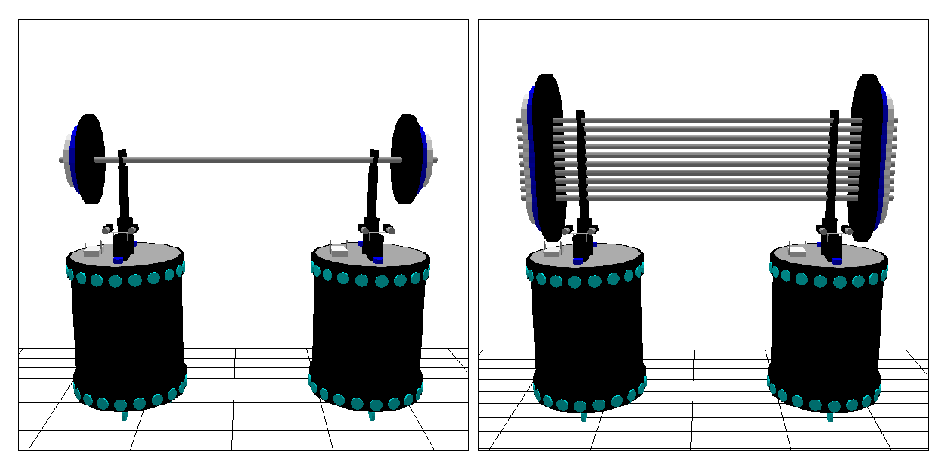
\includegraphics[width=10cm]{FIG/Constraint/halteres.eps}
}
\centerline{
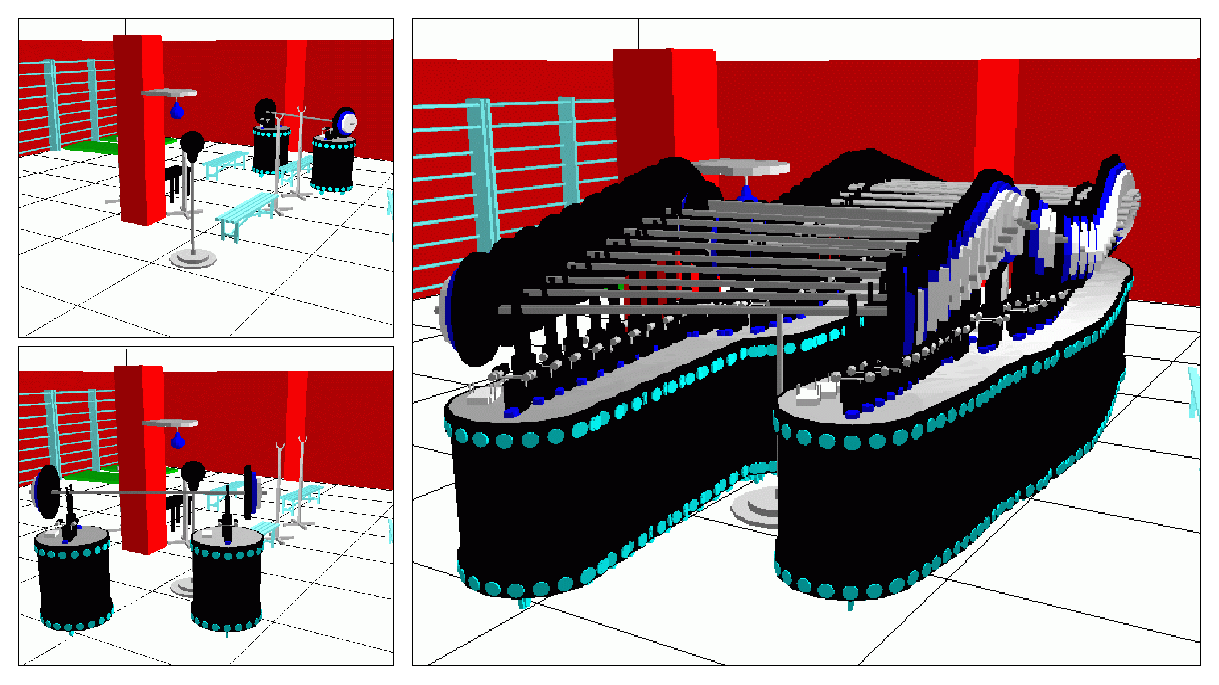
\includegraphics[width=10cm]{FIG/Constraint/halteres2.eps}
}
\caption{\label{fig:halteres} Two holonomic robots cooperating in a
task. The bar with the weighs must stay horizontal, so the hydraulic
bars of the robots must move at the same time.}
\end{figure}


Another example of application of this kinematic constraint would be
the incorporation of natural effects in the simulating model. The
constraint represented in Figure~\ref{fig:dedos} corresponds to the
natural motion of a finger. There is a relationship between the
movement of the phalanges of a hand finger. It could be modeled in a
simple way as a linear relationship.

\begin{figure}[ht!]
%\vspace{15.0mm}
\begin{center}
  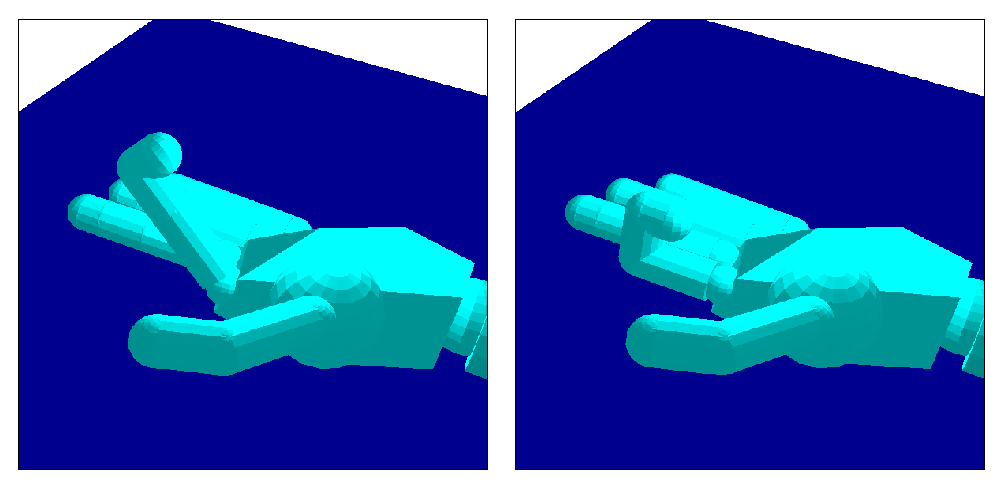
\includegraphics[width=10.0cm]{FIG/Constraint/dedos.eps}
\end{center}
\caption{\label{fig:dedos} Constraint in the movement of a finger. The 
left figure shows an abnormal position for a finger, the right one shows a 
normal situation.}
%\vspace{5.0mm}
\end{figure}


\subsection*{$RRPR$, $4R$ and $3RPR$ linkages}

The $RRPR$, $4R$ nd $3RPR$ linkages are basic planar closed kinematic
chains. Theirs constraint equations are calculated by planar geometry,
likewise theirs motion limits. It must be remarked that {\bf joints
  affected by these constraints must be defined on the same plane}.
Next each one of these linkages will be separately explained.

%\vspace{5.0mm}
\begin{figure}[ht!]
%\vspace{5.0mm}
\begin{center}
\psfrag{teta}[l]{$\theta$} 
\psfrag{chi}[l]{$\psi$}
\psfrag{r}[l]{$r$}
\psfrag{s}[l]{$s$}
\psfrag{g}[l]{$g$}
\psfrag{e}[l]{$e$}
  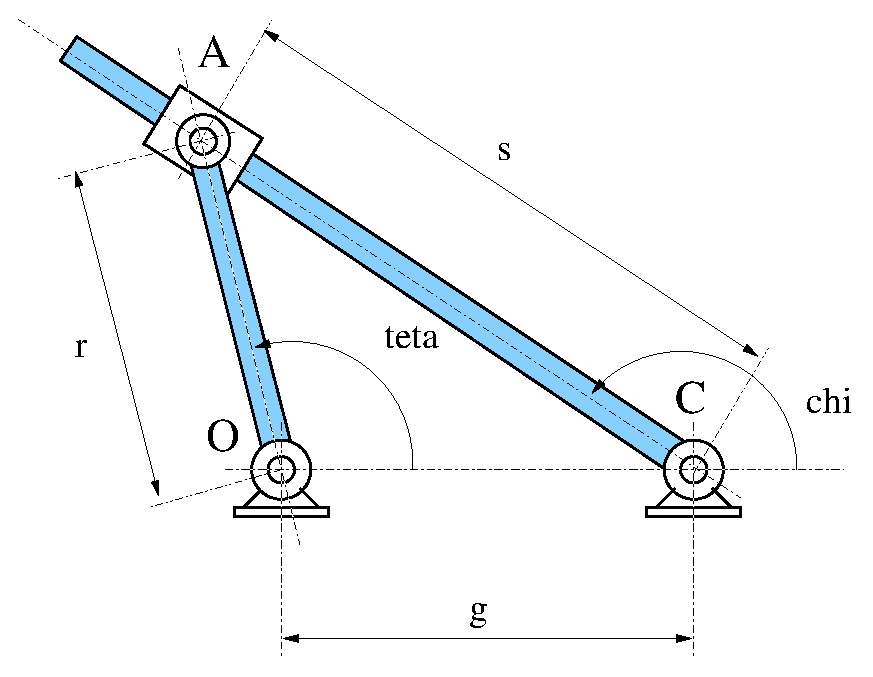
\includegraphics[width=7.0cm]{FIG/Constraint/RRPR2.eps}
\end{center}
\caption{\label{fig:RRPR} The dimensions characterizing an $RRPR$
linkage.}
%\vspace{5.0mm}
\end{figure}


The $RRPR$ linkage is known as a {\em slider-crank} and consist of two
rotating cranks linked by a translating slider. It is a one
degree-of-freedom planar closed chain that is a fundamental machine
element found in everything from automotive engines to door closing
mechanisms.

In the implementation of this constraint in Move3D, the
translation $s$ has been chosen to be the d.o.f. that controls the chain. Therefore,
the joint representing $s$ ($JA$) will be the active joint and the joints
representing $\theta$ ($JO$) and $\psi$ ($JC$) will be the passive
ones. Notice that $JO$ and $JC$ must have the same parent, and $JA$
must be placed in the point corresponding to {\bf A} in the modeling.

\begin{figure}[ht!]
\begin{center}
\psfrag{teta}[l]{$\theta$} 
\psfrag{chi}[l]{$\psi$}
\psfrag{fi}[l]{$\phi$}
\psfrag{a}[l]{$a$}
\psfrag{h}[l]{$h$}
\psfrag{g}[l]{$g$}
\psfrag{b}[l]{$b$}
 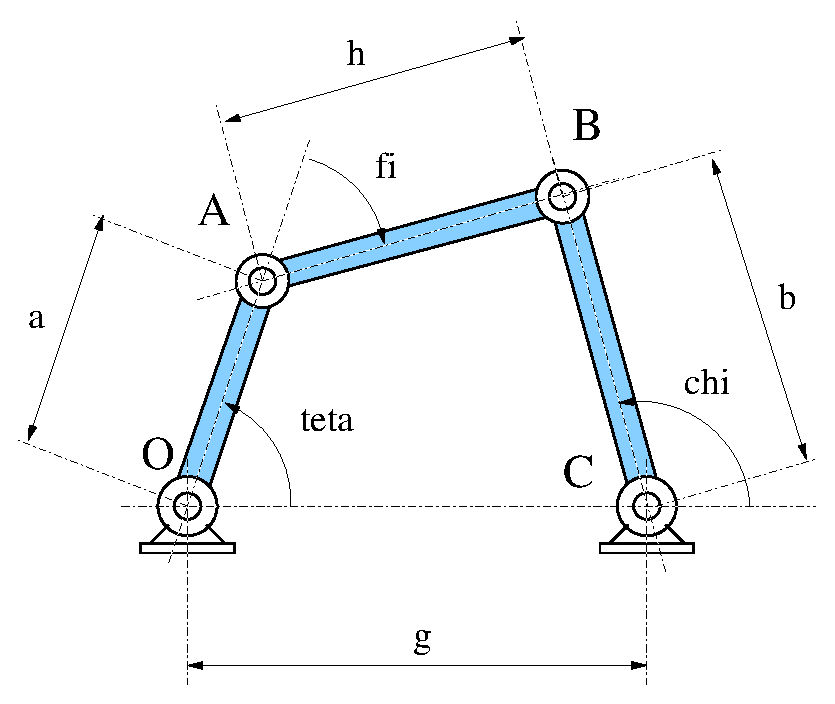
\includegraphics[width=7.0cm]{FIG/Constraint/4R.eps}
\end{center}
\caption{\label{fig:4R} The dimensions characterizing an $4R$ linkage.}
\end{figure}

The $4R$ linkage is a four-rotations planar closed chain. It consist
of an input crank ({\bf OA}), an output crank ({\bf CB}) and a coupler 
({\bf AB}). There is also just one d.o.f. in this fundamental mechanism,
which is the input crank.  

The following remarks must be obeyed for the modeling of this chain:
$JO$ and $JC$ must be defined on the same solid; the coupler must be
defined from the input crank, that is, the chain is cut at {\bf B};
the joint $JB$ can be placed at the end of the output crank or at the
end of the coupler, but this joint is necessary in order to calculate
lengths of the links.

The $3RPR$ linkage can be seen as a $4R$ linkage where the length of
the output crank is variable. It is, therefore, a two d.o.f. planar
closed chain. These two active joints corresponds to the input crank
({\bf OA}) and the translating slider placed at {\bf B} on the output
crank. 

\begin{figure}[ht!]
\begin{center}
\psfrag{teta}[l]{$\theta$} 
\psfrag{chi}[l]{$\psi$}
\psfrag{fi}[l]{$\phi$}
\psfrag{a}[l]{$a$}
\psfrag{h}[l]{$h$}
\psfrag{g}[l]{$g$}
\psfrag{s}[l]{$s$}
 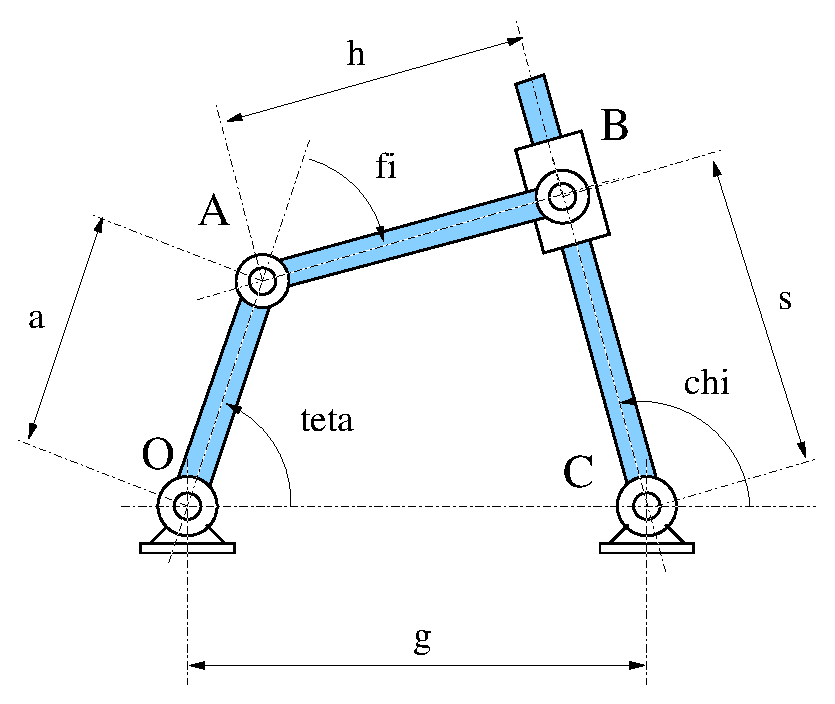
\includegraphics[width=7.0cm]{FIG/Constraint/3RPR.eps}
\end{center}
\caption{\label{fig:3RPR} The dimensions characterizing an $3RPR$ linkage.}
\end{figure}

The remarks for the modeling are similar to the ones made for the
$4R$ linkage, but in this case $JB$ is the translating joint, and it
must be defined from the output crank.

Now, some of the results obtained before the
implementation of these constraints in Move3D will be shown. Figures~\ref{fig:excavator}
represents the model of an hydraulic excavator. The motion of its arm
is controlled by the hydraulic systems, so there are 3 d.o.f.. This
mechanical system contains four closed kinematic chains. Three of them
are the hydraulic systems, and the fourth one is the mechanism for the
motion of the bucket. The hydraulic systems can be modeled as $RRPR$
linkages where the translating crank is the hydraulic bar. The
mechanism of the bucket is a $4R$ linkage. But the third hydraulic
system and the mechanism of the bucket are linked, so we really have
two single closed chains and one double loop closed chain.

\begin{figure}[hb!]
\begin{center}
  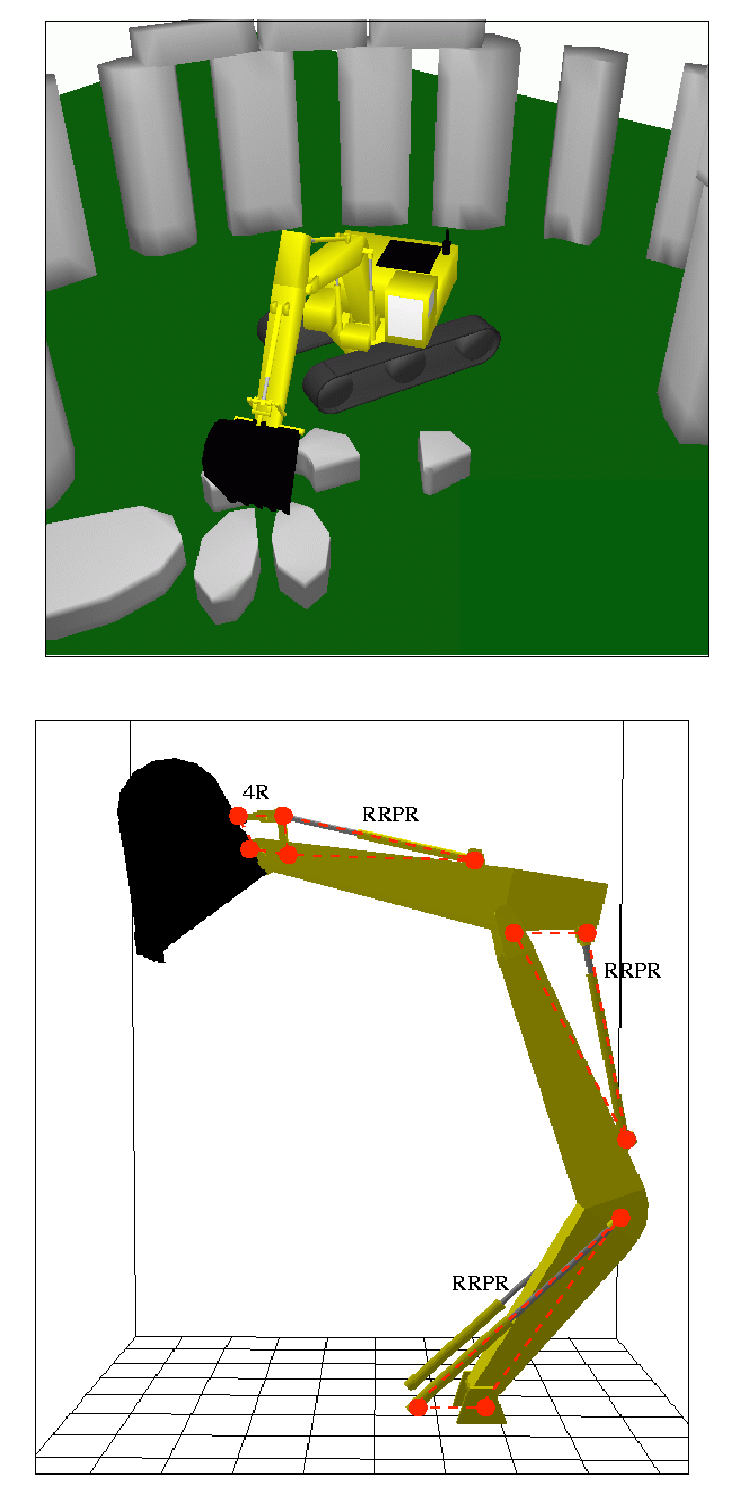
\includegraphics[width=8.1cm]{FIG/Constraint/excavator.eps}
\end{center}
\caption{\label{fig:excavator} Hydraulic excavator. This model
contains two single closed chains and one double loop closed chain. The 
arm, a mechanical system of 19 d.o.f. has been constrained to a system of 3 d.o.f..}
\end{figure}


\begin{figure}[ht!]
\begin{center}
  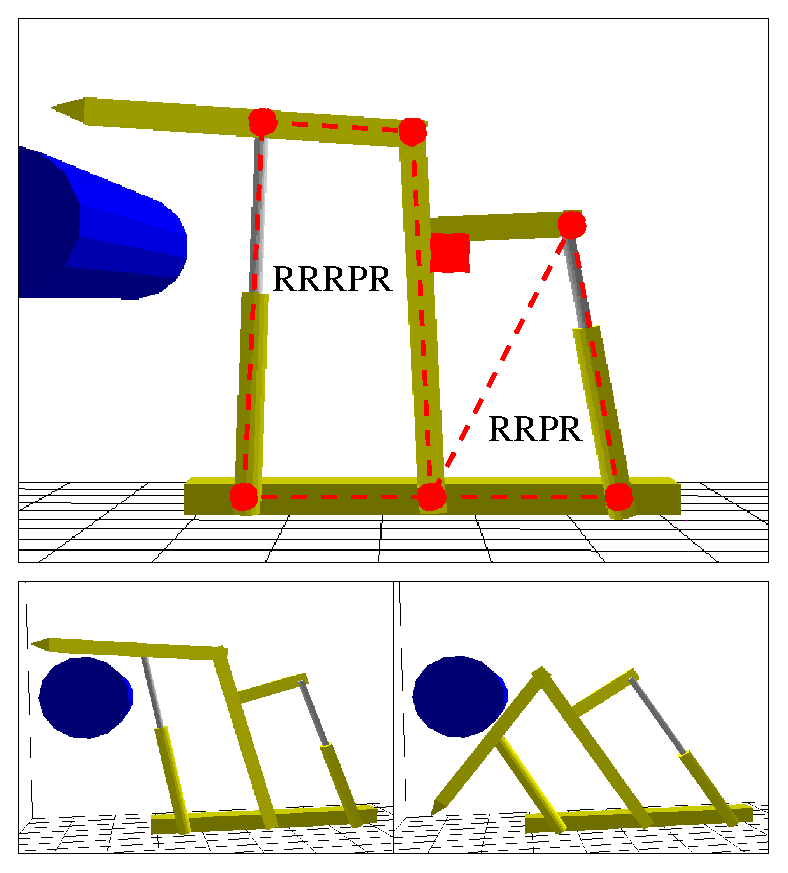
\includegraphics[width=8.0cm]{FIG/Constraint/liegeois.eps}
\end{center}
\caption{\label{fig:liegeois} Manipulator shown in some works of Liegeois.
This two d.o.f. mechanical system consist of a double loop closed chain.} 
\end{figure}

The mechanical system in Figures~\ref{fig:liegeois} is another example
of a double loop closed chain. In this case, the two single chains are 
a $RRPR$ linkage for the rear hydraulic system, and a $3RPR$ linkage
for the front loop.


\subsection*{Contact with ground}

This kinematic constraint represents the case when an object is
required to stay in contact with an obstacle. Particularly, the
implemented constraint corresponds to an object that have to move with
its lowest point sliding on the ground.

The kind of problems which we are mainly interested in are mobile
machines (robots) carrying long objects that have to trail on the
ground. However, the general problem has not been already solved. Just
the last joint of the robot, that is, the joint of the terminal organ
of the robot which grasp the carried object, is going to be
controlled.  This joint must be a revolute joint turning around an
axis perpendicular to the absolute $z$-axis of the scene. This
particular case can be seen as a planar problem.

\begin{figure}[ht!]
\begin{center}
\psfrag{te}[l]{$\theta$} 
\psfrag{li}[l]{$\theta_{JC}$}
\psfrag{de}[l]{$\theta o_{JC}$}
\psfrag{ang}[l]{$\theta_{Object}$}
\psfrag{ant}[l]{$\theta_P$}
\psfrag{d}[l]{$d$}
\psfrag{z_J}[l]{$z_J$} 
\psfrag{z_G}[l]{$z_0$}    
  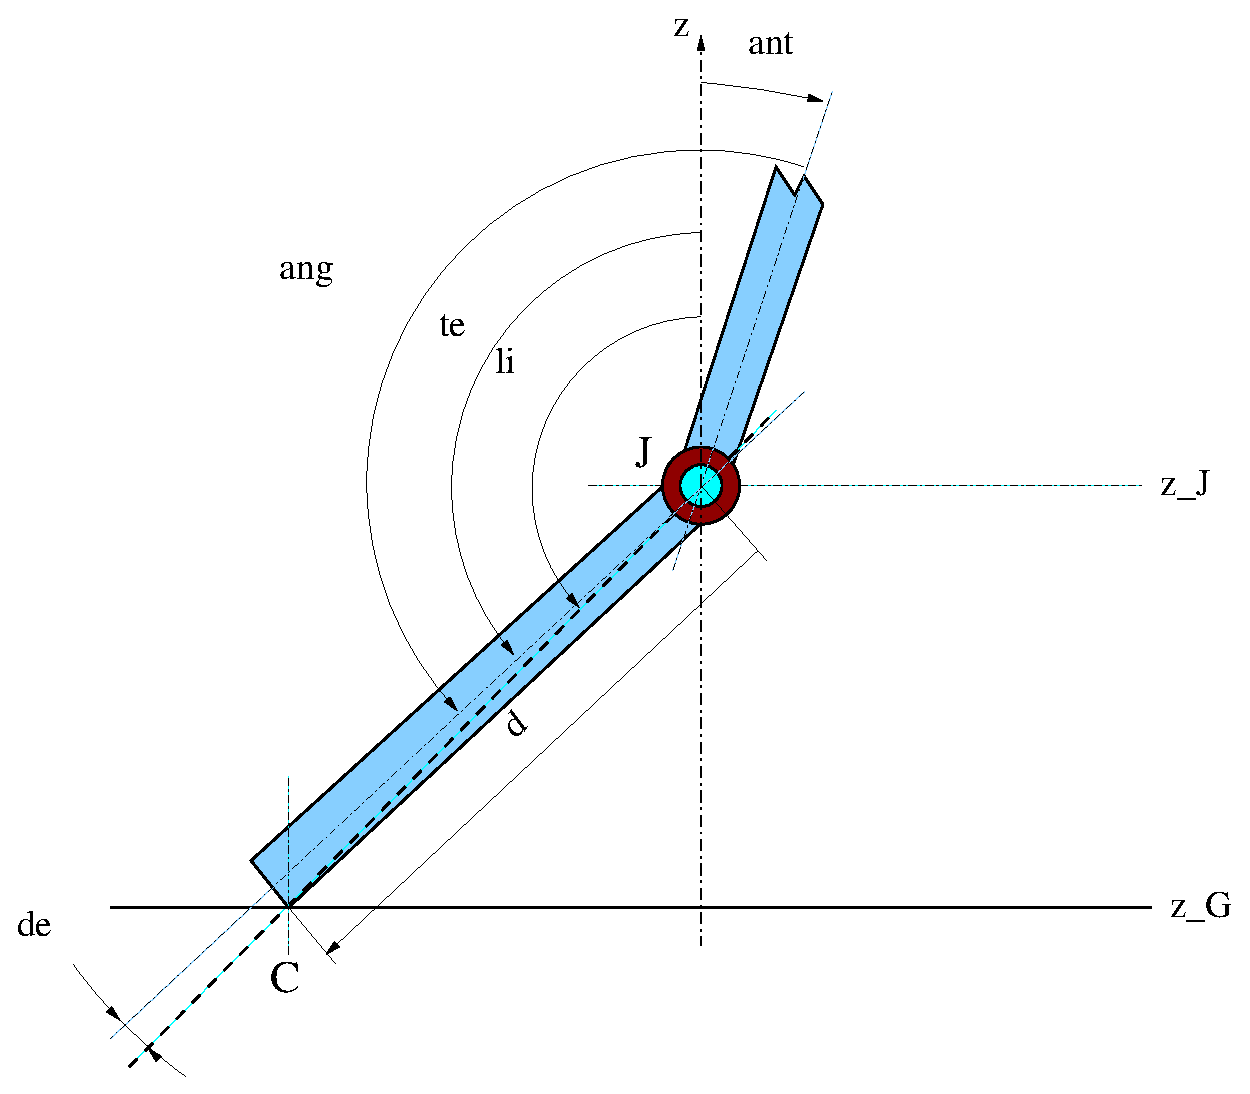
\includegraphics[width=7cm]{FIG/Constraint/ground.eps}
\end{center}
\caption{\label{fig:ground} Variables and references in the analysis.}
\end{figure}

Some remarks for the modeling must be made for this constraint. Let us 
suppose that, for long-shaped objects, the point having to stay
in contact with the ground does not change. In the file containing the
workspace for the path planning with Move3D, the carried object must
be modeled as another body of the robot. Therefore, a joint can be
placed in the point of this `body' that has to slide on the ground.
This joint will be or not a connection with another body, so it will
be not a real joint, but it is necessary to include it in the model.
Let us call it {\bf $J_C$} because it is placed at the point {\bf C}.
It must not be forgotten during the modeling that we are solving a
planar problem. That is to say that the points {\bf J} and {\bf $J_C$}
must be in the same plane, and this plane must be perpendicular to the
rotation axis of the joint at {\bf J}.

\begin{figure}[ht!]
\begin{center}
  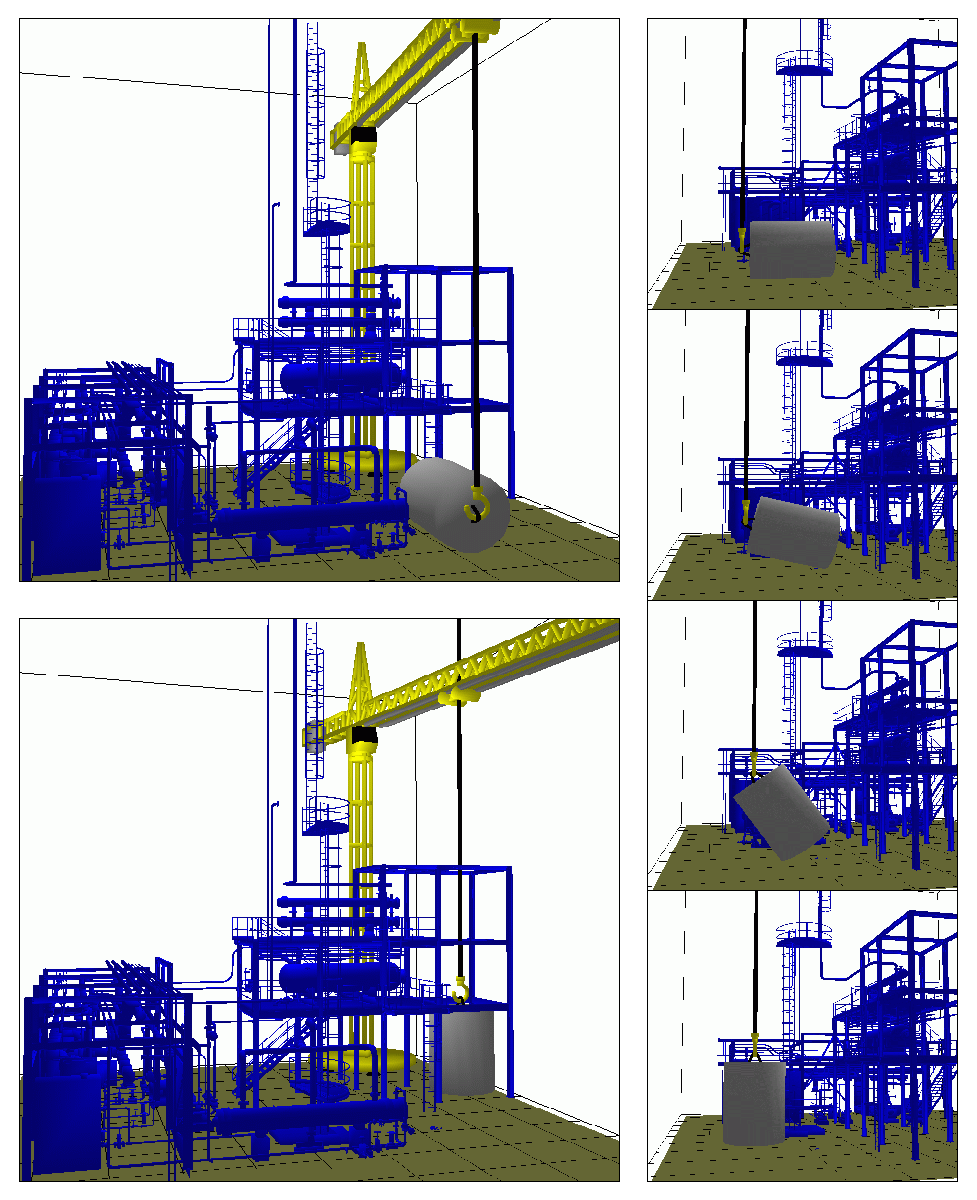
\includegraphics[width=8.0cm]{FIG/Constraint/grue.eps}
\end{center}
\caption{\label{fig:gruaind} A crane has to place a tank into a
metallic structure in an industrial environment. In the initial
configuration, the tank is horizontally placed on the ground. The tank
has to slide on the ground before it reaches the vertical position.}
\end{figure}

Applications of this kind of kinematic constraint are particularly
interesting. For instance, in industrial environments they exist path
planning problems where a moving object must stay in contact with the
ground following physical laws. Figure~\ref{fig:gruaind} shows an
example of one of these problems. The typical example of application,
also usual in the industrial environments, consist in a `robot'
carrying long-shaped objects with a point sliding on the ground. The
example in Figure~\ref{fig:pipe} shows the performance of the planner
handling this kind of kinematic constraint.

\begin{figure}[ht!]
\centerline{
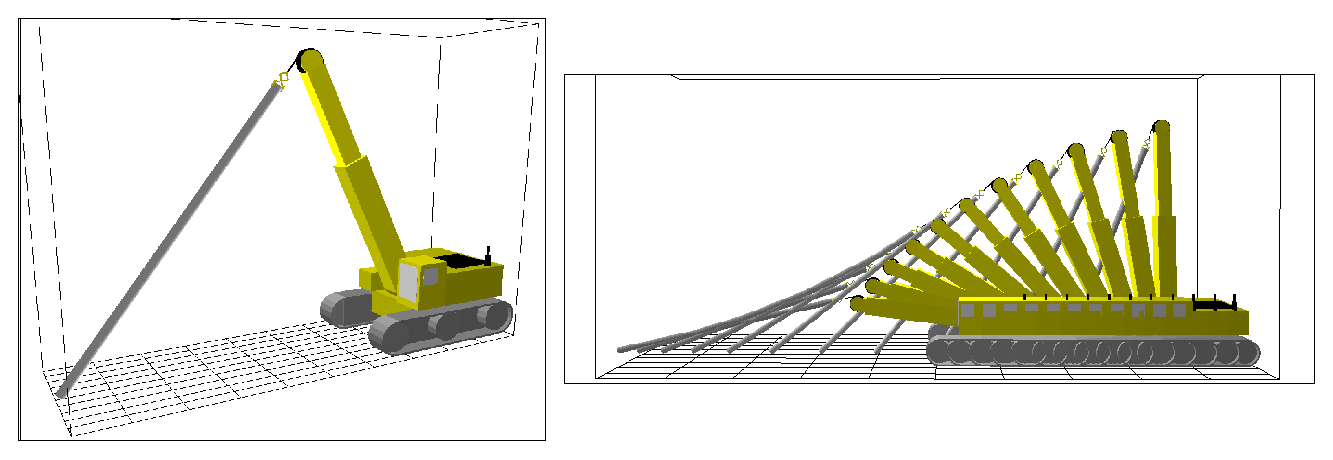
\includegraphics[width=15cm]{FIG/Constraint/pipe12.eps}
}
\caption{\label{fig:pipe} A telescopic handler carries a long
pipe. The lowest extreme of the pipe must stay in contact with the
ground all along the path.}
\end{figure}

\subsection*{Car front wheels}

\begin{figure}[ht!]
\begin{center}
\psfrag{t}[l]{$\theta$} 
\psfrag{O}[l]{O} 
\psfrag{P}[l]{P}    
  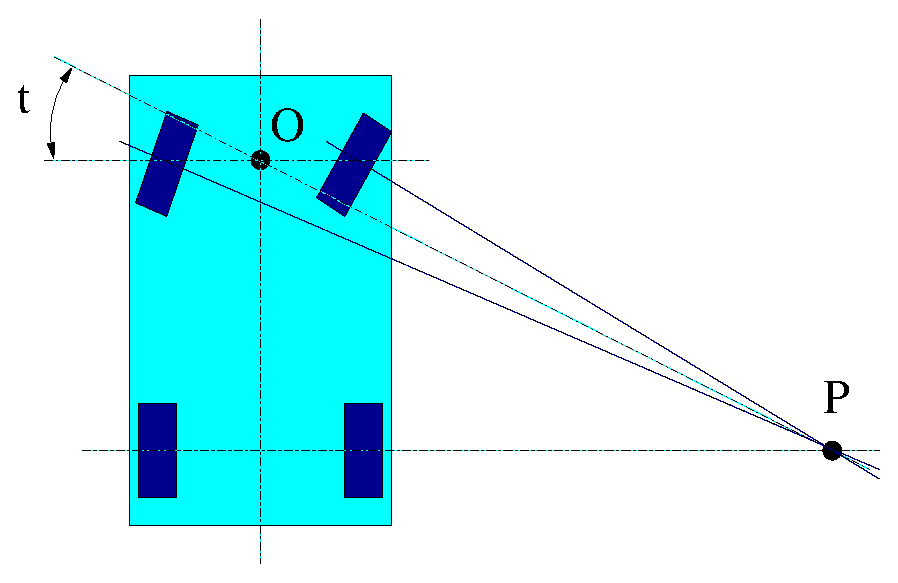
\includegraphics[width=8cm]{FIG/Constraint/carfw.eps}
\end{center}
\caption{\label{fig:carfw} Geometric law for the angles of the car 
  front wheels.}
\end{figure}

This kinematic constraint will be applied to cars. A car can be
modeled as a robot towing a trailer. The steering column of the car is
represented by the robot and the body of the car is represented by the
trailer (see Chapter~\ref{methode-local}). The angle of each
front wheel is then computed as shown on Figure~\ref{fig:carfw}.
That is, the axes of all the wheels (front and rear) must coincide in
a same point {\bf P}.  This point is also the intersection between the
rear wheels axis and the line passing trough the car turning center
(steering column) {\bf O} and having the car turning angle $\theta$.
This point {\bf O} represents the joint between the robot and the
trailer.

Figure~\ref{fig:LegoCar} shows the model of a car
within this constraint has been successfully tried.



\begin{figure}[htb!]
\begin{center}
  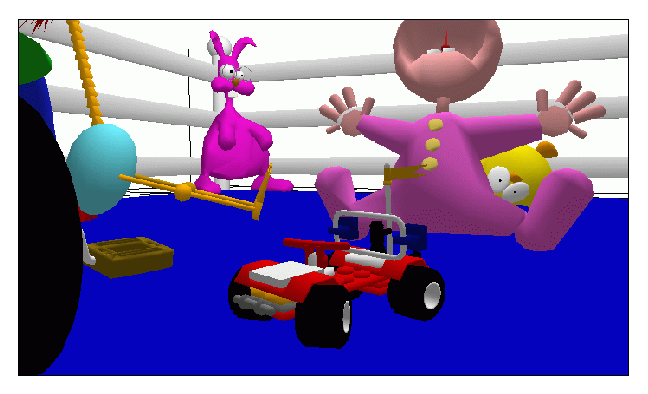
\includegraphics[width=8cm]{FIG/Constraint/LegoCar.eps}
\end{center}
\caption{\label{fig:LegoCar} Three-dimensional model of a LegoCar.}
\end{figure}


\subsection*{Planar closed chain}

A general analytical solution for a planar closed
chain is used in this constraint. It is known that for a n-bar planar mechanism, the number of
d.o.f is n-3. The base of the mechanical system is considered as one
of the bars, then it becomes a (n-1)-bar mechanism with (n-1)-2 d.o.f.
The chosen method to solve this geometrical problem
consist of cutting the loop in two parts. At one side we leave a 2-bar
open chain. At the other side we will have another open chain with the
rest of the elements. The two joints of the first part will be the
passive joints (the two lost d.o.f.), while the joints the other part
remain active. The angles of the passive joints are calculated by
trigonometric laws in order to close the loop.

\begin{figure}[h!]
\begin{center}
\psfrag{a}[l]{$\theta 1$} 
\psfrag{b}[l]{$\theta 2$}
\psfrag{chi}[l]{$\psi$}
\psfrag{fi}[l]{$\phi$}
\psfrag{d}[l]{$d$}
\psfrag{any planar open chain}[l]{any planar open chain}
  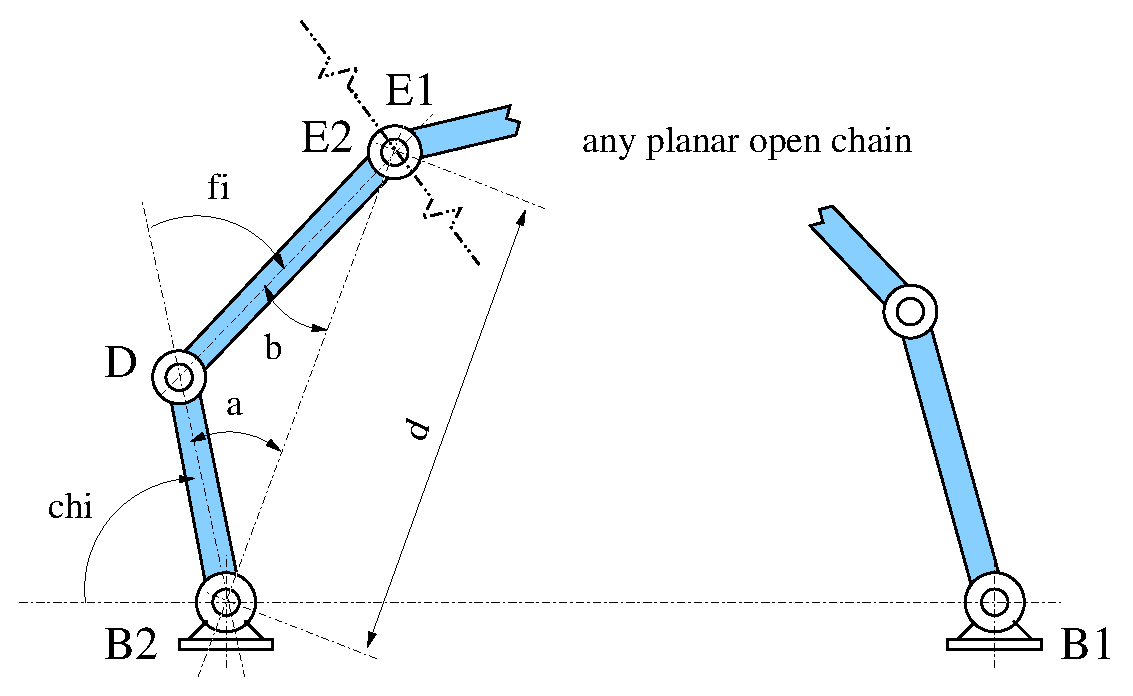
\includegraphics[width=7cm]{FIG/Constraint/plclch.eps}
\end{center}
\caption{\label{fig:plclch} Variables and references in the analysis.}
\end{figure}

Figure~\ref{fig:plclch} represents the way how a mechanical system 
containing this kinematic constraint must be modeled. Joints ({\bf E1}
and {\bf E2}) must be placed at the end of each open chain.

Figure~\ref{fig:cad8pas} shows the performance of Move3D solving a 
path planning problem for a 8-bar closed chain.

\begin{figure}[h!]
\begin{center}
  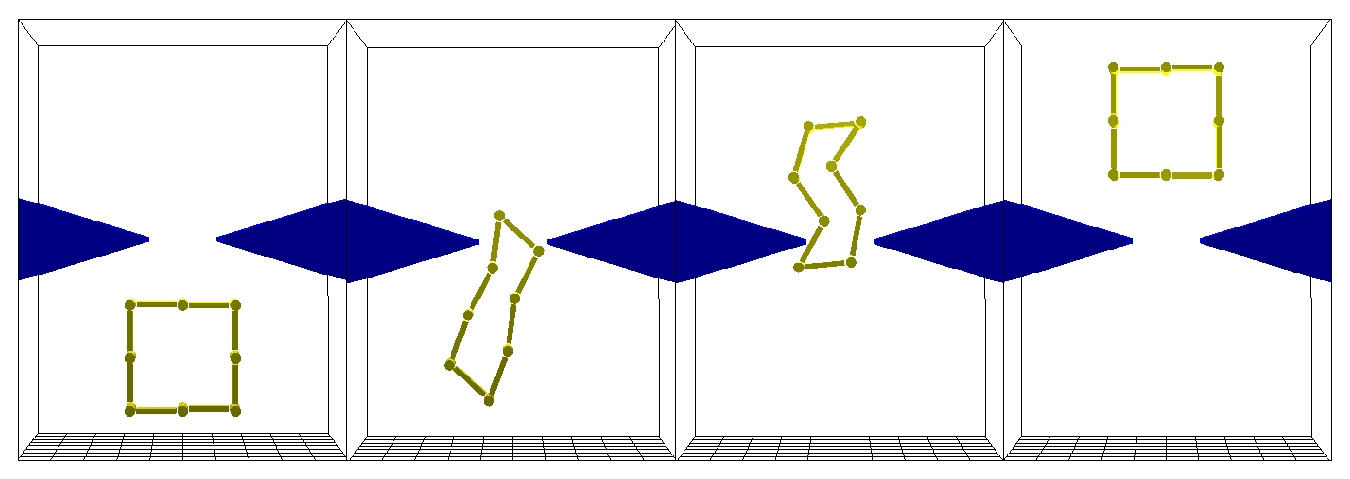
\includegraphics[width=10cm]{FIG/Constraint/cad8pas.eps}
\end{center}
\caption{\label{fig:cad8pas} Some sequences of the solution given
  by Move3D for a 8-bar closed chain that has to find a path trough a
  narrow passage.}
\end{figure}

\section{How to use them}

Kinematic constraints can be set in the mechanical system in two ways: 
they can be directly set in the model input file ({\tt .p3d}), or they can
be set once Move3D is running. Next, this two
possibilities are explained.

\subsection*{Kinematic constraints in the {\tt .p3d} file}

Constraints can be introduced in the mechanical system by adding command 
lines at the end of the model input file. These command lines have the 
following structure: 

\hspace{-4.0mm}
{\tt p3d\_constraint \footnotesize cntrt\_name npasjnts \{pj1...pjn\} nactjnts
  \{aj1...ajn\} nc \{c1...cn\} no \{o1...on\}} \index{p3d\_constraint} \\

where:
\begin{tabbing}
>>>\=>>>>>>>>>>>>> \= \kill
\> - {\tt cntrt\_name} \>: is the name of the kinematic constraint to 
  be set.\\
\> - {\tt npasjnts}   \>: is the number of passive joints.\\
\> - {\tt \{pj1...pjn\}}\>: are the indexes corresponding to each one of 
  the passive joints.\\
\> - {\tt nactjnts}   \>: is the number of active joints.\\
\> - {\tt \{aj1...ajn\}}\>: are the indexes corresponding to each one of 
  the active joints.\\
\> - {\tt nc}         \>: is the number of (real) constant parameters.\\
\> - {\tt \{c1...cn\}}  \>: are the constant parameters of the
  constraint.\\
\> - {\tt no}          \>: is the number of other (integer) constant parameters.\\
\> - {\tt \{o1...on\}}   \>: are integer constant parameters of the
  constraint.\\
\end{tabbing}

  
For each one of the kinematic constraints explained in
the last section, the parameters of this command line are as follows
(see figures in last section for the references of points and joints):

\begin{tabbing}
>\=>>\=>>>>>>>>>>>>\=>>>\= \kill
\>{\normalsize \bf Linear relationship between two d.o.f.} \\
\>\>\\
\>\>{\bf \tt cntrt\_name} \>: {\tt p3d\_lin\_rel\_dofs}\\
\>\>{\bf \tt npasjnts} \>: 1\\
\>\>{\bf \tt pj1} \>: index of the joint to be controlled ($JA$)\\
\>\>{\bf \tt nactjnts} \>: 1\\
\>\>{\bf \tt aj1} \>: index of the joint that controls $JA$ ($JB$)\\
\>\>{\bf \tt nc} \>: 2\\
\>\>{\bf \tt c1} \>: linear relationship coefficient ($K$)\\
\>\>{\bf \tt c2} \>: offset ($C$)\\
\>\>{\bf \tt no} \>: 0\\
\>\>\\
\>{\normalsize \bf $RRPR$ linkage} \\
\>\>\\
\>\>{\bf \tt cntrt\_name} \>: {\tt p3d\_RRPRlnk}\\
\>\>{\bf \tt npasjnts} \>: 2\\
\>\>{\bf \tt pj1} \>: index of the joint corresponding to {\bf O}\\
\>\>{\bf \tt pj2} \>: index of the joint corresponding to {\bf C}\\
\>\>{\bf \tt nactjnts} \>: 1\\
\>\>{\bf \tt aj1} \>: index of the translating joint, placed at {\bf A}\\
\>\>{\bf \tt nc} \>: 0\\
\>\>{\bf \tt no} \>: 0\\
\>\>\\
\>{\normalsize \bf $4R$ linkage} \\
\>\>\\
\>\>{\bf \tt cntrt\_name} \>: {\tt p3d\_4Rlnk}\\
\>\>{\bf \tt npasjnts} \>: 3\\
\>\>{\bf \tt pj1} \>: index of the joint corresponding to {\bf A}\\
\>\>{\bf \tt pj2} \>: index of the joint corresponding to {\bf B}\\
\>\>{\bf \tt pj3} \>: index of the joint corresponding to {\bf C}\\
\>\>{\bf \tt nactjnts} \>: 1\\
\>\>{\bf \tt aj1} \>: index of the joint corresponding to {\bf O}\\
\>\>{\bf \tt nc} \>: 0\\
\>\>{\bf \tt no} \>: 0\\
\>\>\\
\>{\normalsize \bf $3RPR$ linkage} \\
\>\>\\
\>\>{\bf \tt cntrt\_name} \>: {\tt p3d\_3RPRlnk}\\
\>\>{\bf \tt npasjnts} \>: 2\\
\>\>{\bf \tt pj1} \>: index of the joint corresponding to {\bf A}\\
\>\>{\bf \tt pj2} \>: index of the joint corresponding to {\bf C}\\
\>\>{\bf \tt nactjnts} \>: 2\\
\>\>{\bf \tt aj1} \>: index of the joint corresponding to {\bf O}\\
\>\>{\bf \tt aj2} \>: index of the translating joint, placed at {\bf B}\\
\>\>{\bf \tt nc} \>: 0\\
\>\>{\bf \tt no} \>: 0\\
\>\>\\
\>{\normalsize \bf Contact with ground} \\
\>\>\\
\>\>{\bf \tt cntrt\_name} \>: {\tt p3d\_jnt\_on\_ground}\\
\>\>{\bf \tt npasjnts} \>: 1\\
\>\>{\bf \tt pj1} \>: index of the joint sliding on the ground ($J_C$)\\
\>\>{\bf \tt nactjnts} \>: 0\\
\>\>{\bf \tt nc} \>: 2\\
\>\>{\bf \tt c1} \>: height ($z$) of the ground\\
\>\>{\bf \tt c2} \>: offset with relation to the horizontal plane
when the body is hanging\\
\>\>{\bf \tt no} \>: 3  (for these variables: 0 == OFF, 1 == ON)\\
\>\>{\bf \tt o1} \>: $J_C$ turns in the negative direction\\
\>\>{\bf \tt o2} \>: $J_C$ changes the turning direction depending on
the position of the rest\\\>\>\>\> of bodies of the robot\\
\>\>{\bf \tt o3} \>: the carried body must stay on the ground (it can
not be hung)\\
\>\>\\
\>{\normalsize \bf Car front wheels} \\
\>\>\\
\>\>{\bf \tt cntrt\_name} \>: {\tt p3d\_car\_front\_wheels}\\
\>\>{\bf \tt npasjnts} \>: 2\\
\>\>{\bf \tt pj1} \>: index of the joint corresponding to the right wheel\\
\>\>{\bf \tt pj2} \>: index of the joint corresponding to the left wheel\\
\>\>{\bf \tt nactjnts} \>: 1\\
\>\>{\bf \tt aj1} \>: index of the joint corresponding to the steering
column {\bf O}\\
\>\>{\bf \tt nc} \>: 2\\
\>\>{\bf \tt c1} \>: distance between front and rear wheels axes\\
\>\>{\bf \tt c2} \>: distance between front wheels\\
\>\>{\bf \tt no} \>: 0\\
\>\>\\
\>{\normalsize \bf Planar closed chain} \\
\>\>\\
\>\>{\bf \tt cntrt\_name} \>: {\tt p3d\_planar\_closed\_chain}\\
\>\>{\bf \tt npasjnts} \>: 2\\
\>\>{\bf \tt pj1} \>: index of the last joint of the controllable (active) half-chain {\bf E1}\\
\>\>{\bf \tt pj2} \>: index of the last joint of the non-controllable (passive) half-chain {\bf E2}\\
\>\>{\bf \tt nactjnts} \>: 1\\
\>\>{\bf \tt aj1} \>: index of the first joint of the controllable half-chain {\bf B1}\\
\>\>{\bf \tt nc} \>: 0\\
\>\>{\bf \tt no} \>: 0\\
\end{tabbing}


\subsection*{Setting and modification of constraints while Move3D is running}

The access to the kinematic constraints, while Move3D is running, is
got from the so called button in the robot control window. This button 
generates the {\em kinematic constraints window} (see
Figure~\ref{fig:kcwin}). This window allows the user to manage
three operations:

\begin{figure}[b!]
\begin{center}
  \includegraphics[width=7.9cm]{FIG/Constraint/kcwin.ps}
\end{center}
\caption{\label{fig:kcwin} Kinematic constraints window. In this
  case, the list of constraints corresponds to the model of the
  excavator arm (see Figure~\ref{fig:excavator}).}
\end{figure}

\begin{itemize}
\item {\bf Activation and deactivation of constraints :} \\
Buttons placed at the left on the kinematic constraints window allow
to activate (pushed) or deactivate (released) any of the already set
constraints. It is important to remark at this point that two kinematic
constraints having the same passive joints can not be active at the
same time.
\item {\bf Modification of some of the parameters of constraints:} \\
A window containing the parameters of each one of the listed constrains 
appears by pushing its corresponding button at the right of the
kinematic constraints window. In this window, the user can modify
some of the parameters of the constraint. Parameters related to joints 
indexes are forbidden to be changed. Upper part of Figure~\ref{fig:jogwins}
represents an example of these windows.
\item {\bf Setting of new constraints:} \\
Kinematic constraints non-included in the model input file can be
introduced in the mechanical system during the running of Move3D. The
{\em kinematic constraints setting window} appears by pushing the button
``NEW'' on the kinematic constraints window. This window contains the 
list of the kinematic constraints types treated in Move3D. Buttons
placed at the right on this window generate the setting windows of
each one of them. The parameters appearing in these setting windows
have been explained in Section ``Treated constraints''. New
constraints containing wrong parameters will not be set, and an error
message will be displayed. Bottom part of Figure~\ref{fig:jogwins} illustrates
the process for a new constraint setting.
\end{itemize}

\begin{figure}[h!]
\begin{center}
  \includegraphics[width=14.0cm]{FIG/Constraint/jogwins.eps}
\end{center}
\caption{\label{fig:jogwins} Kinematic constraints window, kinematic
  constraints setting window, window containing the parameters of a
  constraint and setting window of a constraint.}
\end{figure}
 

\section{Implementation}

When a kinematic constraint is set, its data structure is
generated. This data structure contains all the necessary information
for the treatment of the constraint. The representation in C language
of this structure is:
{\tt
\begin{tabbing}
>>>>>>>>>>>>\=>>\=>>>>>>>>>>>> \= \kill
\>typedef struct cntrt \{ \\ 
\>\>  int       \> num;\\
\>\>  char      \> namecntrt[40];\\
\>\>  int       \> active;\\
\>\>  int       \> (*fct\_cntrt)(struct cntrt *ct);\\
\>\>  int       \> nactjnts, npasjnts;\\
\>\>  int       \> ndval, nival;\\
\>\>  int       \> actjnts[MAX\_ARGU\_CNTRT];\\
\>\>  int       \> actjnt\_state[MAX\_ARGU\_CNTRT];\\
\>\>  int       \> pasjnts[MAX\_ARGU\_CNTRT];\\
\>\>  int       \> argu\_i[MAX\_ARGU\_CNTRT];\\
\>\>  double    \> argu\_d[MAX\_ARGU\_CNTRT];\\
\>\>  int       \> col\_pairs[2][MAX\_ARGU\_CNTRT];\\
\>\>  struct cntrt \> *next\_cntrt;\\
\>\>  struct cntrt \> *prev\_cntrt;\\
\>\>  int       \> enchained\_J[MAX\_ARGU\_CNTRT];\\
\>\>  int       \> nenchained;\\
\>\>  struct cntrt \> **enchained;\\
\>\} p3d\_cntrt,*pp3d\_cntrt; \\
\end{tabbing}
}

Some of the members of this data structure have been already
named, and theirs values are directly given by the user. The rest
of them are automatically calculated in the setting function of each
constraint. In order to  allow a further comprehension about how the
implementation of the kinematic constraints is made, these variables
will be briefly explained next.
\begin{itemize}
\item[$-$] The data structure of each robot in the workspace of Move3D contains 
an array of pointers to the data structures of its kinematic
constraints. {\bf \tt num} represents the index of a constraint in this
list.
\item[$-$] {\bf \tt name} contains the name of the constraint.
\item[$-$] {\bf \tt active} is a flag to indicate the state of the constraint
 (activated/deactivated).
\item[$-$] {\bf \tt fct\_cntrt} is a pointer to the function
containing the equations to solve this constraint type.
\item[$-$] {\bf \tt nactjnts} and {\bf \tt npasjnts} are respectively the number
  of active and passive joints of the constraint.
\item[$-$] {\bf \tt ndval} and {\bf \tt nival} are respectively the
  number of real and integer constant parameters of the constraint
  that are given by the user.
\item[$-$] {\bf \tt actjnts} and {\bf \tt pasjnts} are arrays containing the indexes of 
the active and passive joints in this constraint.
\item[$-$] {\bf \tt actjnt\_state} is an array of flags for the active joints of
the constraint. A flag set to $0$ means that the corresponding joints
is involved in a previously defined constraint.
\item[$-$] {\bf \tt argu\_i} and {\bf \tt argu\_d} contain respectively integer and
real constant parameters of the kinematic constraint. Some of these
parameters are the ones introduced by the user. The rest are
automatically calculated. The kind of these calculated constants are, for
example: flags, distances between joints or values to refer angles.
\item[$-$] {\bf \tt col\_pairs} is used to stock information for the 
  deactivation of pairs of bodies for the collision checking.
\item[$-$] {\bf \tt next\_cntrt} and {\bf \tt prev\_cntrt} are
  pointers to the next and preceding constraints in the above
  mentioned list.
\item[$-$] {\bf \tt enchained\_J}, {\bf \tt nenchained} and {\bf \tt enchained} are used for 
  the treatment of {\em multi-constraints}. This concept will be
  explained later.
\end{itemize}


Two special remarks can be made at this point. These remarks ascribe
collision checking and multi-constraints.

Pairs of consecutive bodies
of a robot are deactivated for the collision checking in Move3D. This
same rule must be followed, for instance, when a kinematic chain is
closed. In this case, collisions between the pair of bodies closing the
chain have not to be tested. Deactivation of pairs affected by
kinematic constraints is carried out form the information stocked in the 
matrix {\tt col\_pairs}.

A special treatment of kinematic constraints have to be made when they
are {\em enchained}. A multi-constraint can be defined as several
kinematic constraints where active joints of some of them are passive
joints for some others. Two kinematic constraints obeying this property are
told to be enchained. An example of enchained constraints are
multi-loop closed chains. Notice that {\bf constraints to
  be enchained must be set in order}, that is to say: if an active
joint in a constraint is a passive joint in another one, this last
constraint must be defined first.


\section{New kinematic constraints}

The way how the treatment of kinematic constraints has been
implemented in Move3D allows that new constraints will be easily added
to the software. The work to do for this purpose have to be developed in the files {\bf
  FORMconstraints.c} and {\bf p3d\_constraints.c}. The first one
contains all the functions related with interface windows. If a new
constraint is wanted to be added, its related functions in this file
will be easily programmed by following the same procedure that for the
rest of constraints. The functions to be added in file {\bf
  p3d\_constraints.c} are the function for the setting of the new
constraint and the one containing its geometric constraint
equation(s). The calculations of the parameters related with the
constraint that are not going to change during the current running of Move3D
have to be made just once. These operations must be placed in the
setting function. The rest of the operations have to be made each time 
that the function with the constraint equation(s) is called, so they
must be placed inside it.



\clearemptydoublepage
\def\hsp{\hspace*{1cm}}

\chapter{Steering methods and local paths}
\label{methode-local}
\def\CS{{\cal C}}

Local path is the element that encodes elementary motion in Move3D:
trajectories are concatenations of local paths, edges of roadmaps
contain local paths. A local path for a given robot is produced by a
local method. In this chapter, we first give a definition of what we
mean by local path. Then we show how different types of local paths
can be handled by Move3D. Finally, we describe the different steering
methods implemented within the software.

\section{Definition of local path and steering method}

\paragraph{Definition and parameterizations of local path.}
A {\em local path} for a robot $r$ is a continuous curve in the
configuration space of the robot and defined over an interval $[0,U]$:
$$
\begin{array}{lcll}
lp: & [0,U] & \rightarrow & \CS \\
    & u &\rightarrow & lp(u)
\end{array}
$$
In the rest of this chapter, $u$ is called the default parameter (or
parameter) of the local path $lp$ and $U$ the parameter range of $lp$.

 The curve can also be parameterized by length (or
  by pseudo-length), 

In addition to the default parameterization, a length parameterization
can be defined. This parameterization has to be defined by the
developper.  The length parameterization is mainly used for optimizing
trajectories.  The optimizing function picks random configurations
over a list of successive local paths. The length parameterization
ensures us that longer local paths are more likely to be chosen than
smaller ones. The length parameterization can be the same as the
default parameterization u.

The length parameter is defined from the default parameter $u$ by an
increasing function $d$ from $[0,U]$ to an interval $[0,L]$. $L=d(U)$
is called the length of the local path. It does not necessarily represent 
a real length. 

\paragraph{Steering method.}
A steering method is a function that maps, to a pair of configurations, a
local path between these configurations. The simplest steering method is the 
linear one. It connects the two configurations by a  straight line in the
space of configuration parameters.
Some robots are subjected to kinematic constraints such as rolling
without slipping for wheeled mobile robots or moving only one degree
of freedom at a time for a rolling bridge. These kinematic constraints
are not specified in the description of the mechanical system. They
are taken into account by the local method. For instance Reeds and Shepp 
steering method builds curves composed of straight lines and arc of circles
for a carlike robot.

\section{Representation of a local path}
\label{sec:representation}

Local paths are encoded by the data-structure {\tt
  p3d\_localpath}\index{Data structures!p3d\_localpath}

A local path is encoded by a variable of type {\tt p3d\_localpath}. This
structure contains 3 types of fields:
\begin{itemize}
\item data generic to any local path,
\item a pointer to data specific to the type of local path
\item pointers to functions specific to the type of local path.
\end{itemize}

The structure {\tt p3d\_localpath} is like an abstract class in an
object-oriented langage. The specific functions are methods associated
to each derived class (each type of local path).

We enumerate now the main fields of the structure {p3d\_localpath}.

\subsubsection*{data generic to any local path.}
\begin{itemize}
\item {\tt type\_lp}: type of local path (linear, reeds and shepp,...).
\item {\tt range\_param}: parameter range of the local path.
\item {\tt length\_lp}: range of the length parameterization.
\end{itemize}

\subsubsection*{specific methods associated to a local path}
\begin{itemize}
\item {\tt length}: computes the length of the local path.
\item {\tt copy}: copies the local path.
\item {\tt extract}: extracts from a given local path the part included between two values of the length parameter of the local path.
\item {\tt destroy}: destroyes the local path.
\item {\tt config\_at\_distance}: computes the configuration at a given
  distance along the local path.
\item {\tt config\_at\_param}: computes the configuration at a given
  parameter along the local path.
\item {\tt stay\_within\_dist}: given the distance of each body of the
  robot to the obstacles, and a position on a local path, this
  function computes an interval of default parameter that ensures the
  user that each body does not move by more than its specified
  distance when the parameter stays in this interval.
\item {\tt cost}: computes the cost of a local path. This cost is used
  in $A^{*}$ procedure to find the best path in the roadmap and during
  optimization to replace a part of a path by a new local path if this
  latter has lower cost.
\item {\tt simplify}: This function does nothing for most local
  paths. given two successive local paths. When two Reeds and Shepp
  local paths are connected, the end of the first one may overlap the
  beginning of the second one. This function detects this kind of
  situation and removes common parts.
\end{itemize}

Data specific to each type of local path are detailled in the
following section.

\section{Local methods implemented within Move3D}

In this section, we describe the various local methods currently supported 
by Move3D. For each of them, we specify the default and length parameterization
used and the data-structures involved.

\subsection{Linear local method}
\label{subsec:linear}

This local method is the simplest one. It connects two configurations
by a straight line in the joint parameter space. If a configuration
parameter represents the rotation angle of a joint without bounds,
along a linear path, this parameter follows the shortest arc between
its initial and final values.

\begin{figure}[ht]
\centerline{\psfig{figure=FIG/localseg.ps, width=6cm}}
\caption{Example of linear local path}
\label{fig:linear-local}
\end{figure}

\subsubsection*{parameterization}

For this type of local path the default and length parameterizations
are the same. Given two configurations, $q_0=(x_0,y_0,z_0,\theta_0,
\phi^{1}_{0},...,\phi^{n}_{0})$ and $q_1=(x_1,y_1,z_1,\theta_1,
\phi^{1}_{1},...,\phi^{n}_{1})$ where the $\phi^i$'s represent the values 
of each joint, we define a distance as follows:
$$
d_{lin}(q_0,q_1) = \sqrt{(x_1-x_0)^2 + (y_1-y_0)^2 + (z_1-z_0)^2 + d_{S^1}(\theta_1-\theta_0)^2 + \sum_{i=1}^{n} d_i(\phi^i_0,\phi^i_1)^2}
$$
where $d_{S^1}$ is the arc length distance over the unit circle, 
\begin{itemize}
\item $d_i(\phi^i_0,\phi^i_1) = |\phi^i_1-\phi^i_0|$ if joint $i$ is a
  translation joint,
  
\item $d_i(\phi^i_0,\phi^i_1) = dist\,|\phi^i_1-\phi^i_0|$ where
  $dist$ is the maximal distance between the points of body $i$ and
  the axis of joint $i$, if this latter is a rotation joint with
  bounds.

\item $d_i(\phi^i_0,\phi^i_1) = dist\, d_{S^1}(\phi^i_0,\phi^i_1)$ if
  joint $i$ is a rotation joint without bounds (i.e. that can rotate
  freely about its axis).
\end{itemize}
The factor $dist$ in front of angular distances makes the linear
distance over the configuration space homogeneous to a length.

\subsubsection*{Data-structure}

Data relative to a linear local path are stored in the following
structure:
\index{Data structures!struct lin\_data}
\index{Data structures!p3d\_lin\_data}
\begin{tabular}{l}{\tt 
struct lin\_data} $\{$ \\
\hsp {\tt configPt q\_init;} \\
\hsp {\tt configPt q\_end;} \\
$\}$ {\tt p3d\_lin\_data, *pp3d\_lin\_data;}\\
\end{tabular}

\noindent
where {\tt q\_init} and {\tt q\_end} are the initial and final
configurations of the local path.

\subsection{Reeds and Shepp + Linear local method}

This local method connects two configurations by Reeds and Shepp
curves in the plane $(x,y)$ for the platform of the robot and linear
curves for the other joints: given two configurations, 
$q_0=(x_0,y_0,z_0,\theta_0, \phi^{1}_{0},...,\phi^{n}_{0})$ and 
$q_1=(x_1,y_1,z_1,\theta_1,\phi^{1}_{1},...,\phi^{n}_{1})$,
$(x_0,y_0,\theta_0)$ and $(x_1,y_1,\theta_1)$ are connected by a
Reeds and Shepp curve of length
$l_{RS}(q_0,q_1)$. $(z_0,\phi^{1}_{0},...,\phi^{n}_{0})$ and
$(z_1,\phi^{1}_{1},...,\phi^{n}_{1})$ are connected
using the linear strategy described in the previous section.

\begin{figure}[ht]
\centerline{\psfig{figure=FIG/RS.ps, width=6cm}}
\caption{Example of Reeds and Shepp + linear local path}
\label{fig:RS-local}
\end{figure}

\subsubsection*{Parameterization}

\paragraph{Default parameterization:} the default parameterization is
the arc-length distance along Reeds and Shepp curve. Thus, the
parameter range is $l_{RS}(q_0,q_1)$.

\paragraph{Length parameterization:} the distance between
configurations $q_0$ and $q_1$ is defined as follows:
$$
d_{RS-lin}(q_0,q_1) = l_{RS}(q_0,q_1) + \sqrt{\sum_{i=1}^{n} d_i(\phi^i_0,\phi^i_1)^2}
$$
where distances $d_i$ are defined as in the previous section. Notice
that the coordinate $z$ does not appear in this distance.

\subsubsection*{Data-structure}

Data relative to a Reeds and Shepp + linear local path are stored in
a list of the following structure:

\index{Data structures!struct rs\_data}
\index{Data structures!p3d\_rs\_data}

\begin{tabular}{l}
{\tt struct rs\_data} $\{$ \\
\hsp {\tt  configPt q\_init;} \\
\hsp {\tt  configPt q\_end;} \\
\hsp {\tt  double centre\_x;} \\
\hsp {\tt  double centre\_y;} \\
\hsp {\tt  double radius;} \\
\hsp {\tt  whichway dir\_rs;} \\
\hsp {\tt  double val\_rs;} \\
\hsp {\tt  rs\_type type\_rs;} \\
\hsp {\tt  struct rs\_data *next\_rs;} \\
\hsp {\tt  struct rs\_data *prev\_rs;} \\
$\}$ {\tt p3d\_rs\_data, *pp3d\_rs\_data;} \\
\end{tabular}

\noindent
each of these structure represent a Reeds and Shepp segment, that is
either a straight line or a left or right turn. 
\begin{itemize}
\item {\tt q\_init} and {\tt q\_end} are the initial and final
  configurations of the RS segment. 
\item {\tt centre\_x}, {\tt centre\_y} is the center of rotation in
case of a right of left turn, $(0,0)$ in case of a straight line. 
\item {\tt radius} is the radius of curvature 
\item {\tt dir\_rs} is the direction (forward or backward) of motion 
\item {\tt val\_rs} is the arc length of the RS segment. 
\item {\tt type\_rs} is the type of segment (right, left turn or
  straight line)
\item {\tt next\_rs} and {\tt prev\_rs} are pointers to the next and
  previous RS segment in the local path.
\end{itemize}

\subsection{Manhattan local method}

A manhattan local path is a path along which only one coordinate moves
at a time. 
Given two configurations, $q_0=(x_0,y_0,z_0,\theta_0,
\phi^{1}_{0},...,\phi^{n}_{0})$ and
$q_1=(x_1,y_1,z_1,\theta_1,\phi^{1}_{1},...,\phi^{n}_{1})$, the
Manhattan local path between them is the concatenation of the
following sub-paths.
\[
\begin{array}{cc}
((1-\alpha)x_0+\alpha x_1,y_0,z_0,\theta_0,\phi^{1}_{0},...,\phi^{n}_{0}) &
0 \leq \alpha \leq 1 \\
(x_1,(1-\alpha)y_0+\alpha y_1,z_0,\theta_0,\phi^{1}_{0},...,\phi^{n}_{0}) &
0 \leq \alpha \leq 1 \\
\vdots & \vdots \\
(x_1,y_1,z_1,\theta_1,\phi^{1}_{1},..., (1-\alpha)\phi^{n}_{0}+\alpha\phi^{n}_{1})& 0 \leq \alpha \leq 1
\end{array}
\]
where the interpolation $(1-\alpha)\phi^{n}_{0}+\alpha\phi^{n}_{1}$
between two angles follows again the shortest arc when possible.
To make the method symmetric, that is, to make it follow the same path
between $q_0$ and $q_1$ as between $q_1$ and $q_0$, we either move the
coordinates in order $x$ to $\phi^{n}$ or in order $\phi^{n}$ to $x$
according to the following criterion:
\begin{itemize}
\item if $x_0<x_1$, move coordinates from $x$ to $\phi^{n}$,
\item if $x_1<x_0$, move coordinates from $\phi^{n}$ to $x$,
\item if $x_1=x_0$, apply criterion to $y_0$ and $y_1$ or to the
  first coordinate different in $q_0$ and $q_1$.
\end{itemize}

\subsubsection*{parameterization}

As for linear local paths, the default and length parameterizations
are the same. Given two configurations, $q_0=(x_0,y_0,z_0,\theta_0,
\phi^{1}_{0},...,\phi^{n}_{0})$ and $q_1=(x_1,y_1,z_1,\theta_1,
\phi^{1}_{1},...,\phi^{n}_{1})$ where the $\phi^i$'s represent the values 
of each joint, we define the Manhattan distance as follows:
$$
d_{manh}(q_0,q_1) = |x_1-x_0| + |y_1-y_0| + |z_1-z_0| + d_{S^1}(\theta_1-\theta_0) + \sum_{i=1}^{n} d_i(\phi^i_0,\phi^i_1)
$$
where $d_{S^1}$ and the $d_i$ are defined in Section~\ref{subsec:linear}.

\subsubsection*{Data-structure}

Data relative to a Manhattan local path are stored in the following
structure:

\index{Data structures!struct manh\_data}
\index{Data structures!p3d\_manh\_data}
\begin{tabular}{l}{\tt 
struct manh\_data} $\{$ \\
\hsp {\tt configPt q\_init;} \\
\hsp {\tt configPt q\_end;} \\
$\}$ {\tt p3d\_manh\_data, *pp3d\_manh\_data;}\\
\end{tabular}

\noindent
where {\tt q\_init} and {\tt q\_end} are the initial and final
configurations of the local path.



\subsection{Trailer local method}

This local method takes into account the nonholonomic constraints of a
robot towing a trailer. Such a system is represented on
figure~\ref{fig:trailer-robot}. 
\begin{figure}[ht]
\centerline{\epsfig{figure=FIG/trailer-robot.eps,width=5cm}}
\caption{A robot with a trailer}
\label{fig:trailer-robot}
\end{figure}
$a$ and $b$ denote the distances between the connection point and
respectively the robot wheel axis and the trailer wheel axis.

The trailer local method uses the property of differential flatness of
the tractor trailer system to build feasible paths between any pair
of configurations of the system. Details about this local method can
be found in~\cite{these-sepanta,these-florent}.

A local path built by this local method is composed of either one
smooth motion or two smooth motions of opposite direction
(backward-forward or forward-backward).

\begin{figure}[ht]
\centerline{\psfig{figure=FIG/trailer.ps, width=6cm}}
\caption{Example of local path computed by the trailer steering method}
\label{fig:trailer-local}
\end{figure}

\subsubsection*{parameterization}

The default parameterization goes from 0 to 1 if the local path is
composed of one part and from 0 to 2 if the local path is composed of
two parts. The length parameterization is proportional to the default
parameterization. The length of a local path is defined
in~\cite{rapport-elodie}. 

\subsubsection*{Data-structure}

Data relative to a trailer local path are stored in the following
structure:

\index{Data structures!struct trailer\_data}
\index{Data structures!p3d\_trailer\_data}
\begin{tabular}{l}
{\tt struct trailer\_data} $\{$ \\
\hsp{\tt   p3d\_sub\_trailer\_data *init\_cusp;} \\
\hsp{\tt   p3d\_sub\_trailer\_data *cusp\_end;} \\
$\}$ {\tt  p3d\_trailer\_data, *pp3d\_trailer\_data;} \\
\end{tabular}

\noindent
where {\tt init\_cusp} and {\tt cusp\_end} are pointers to sub-local
paths of the type convex combination of canonical
curves~\cite{these-florent}. We do not give more details here about how
these sub-local paths are encoded. It would require further
developments that are out of the scope of this document.

\subsubsection*{Motion execution aspects}

The trailer local method is used at LAAS to plan paths for Hilare
towing a trailer. To follow a series of local paths returned by the
local method without stopping between two local paths, the curvature
of the curve followed by the center of the robot has to be continuous.
To make this curvature continuous along a path, we have to store it in
a configuration variable. For that, we define in the configuration
file of the robot a virtual joint attached to the robot and that
encodes this curvature\footnote{In fact, the value of the
  configuration variable of the virtual joint is the derivative of the
  curvature of the flat output w.r.t. an arc-length
  parameterization.}. Figure~\ref{fig:virtual-joint} shows an example
of configuration file for Hilare and its trailer.

\begin{figure}[ht]
\begin{tabular}{l}
{\tt p3d\_beg\_desc P3D\_ROBOT } \\
{\tt p3d\_beg\_desc P3D\_BODY body } \\
\hsp\hsp\hsp $\vdots$ \\
{\tt p3d\_end\_desc} \\
{\tt } \\
{\tt \# derivative of the curvature (-3000 < dK/ds < 3000)} \\
{\tt p3d\_add\_desc\_jnt P3D\_TRANSLATE 0 0 0  0 0 1 0.0 -3000.0 3000.0 0
  0 0} \\
{\tt } \\
{\tt \# angle between the robot and the trailer (-70 deg < phi < 70 deg)} \\
{\tt p3d\_add\_desc\_jnt P3D\_ROTATE -0.65 0 0.92 0 0 1 0.0 -70.0 70.0 0} \\
{\tt } \\
{\tt p3d\_beg\_desc P3D\_BODY trailer} \\
\hsp\hsp\hsp $\vdots$ \\
{\tt p3d\_end\_desc} \\
{\tt p3d\_end\_desc} \\
\end{tabular}
\caption{Example of configuration file for Hilare and its trailer
  ({\tt hilare-trailer.macro}). The first joint is the virtual joint.
  The bounds $[-3000,3000]$ can be set to any value, they are
  recomputed by Move3D. The second joint corresponds to the connection
  between the trailer and the robot.}
\label{fig:virtual-joint}
\end{figure}

\subsubsection*{local method parameters}

Applying the trailer local method to a given robot requires to
initialize some geometric parameters. These parameters are defined in
the configuration file describing the environment and are stored in the
data-structure that describes the robot. These geometric parameters
are the following~:
\begin{itemize}
\item the connection length $a$ and $b$
\item the joint Id corresponding to the trailer connection on the
  robot
\item the virtual joint Id.
\end{itemize}

These geometric parameters are set for each robot in the configuration
file of the scene by the following command~:

\begin{tabular}{l}
{\tt p3d\_sel\_desc\_name P3D\_ROBOT robot\_name} \\
{\tt p3d\_set\_local\_method\_params a b j1 j2}\index{p3d\_set\_local\_method\_params}
 \\
\end{tabular}

where {\tt robot\_name} is the name of the robot to initialize, $a$
and $b$ are the trailer connection lengths defined on
Figure~\ref{fig:trailer-robot}, $j1$ and $j2$ are the joint Id's
corresponding to respectively the trailer connection and the virtual
joint. Let us recall that joints are numbered increasingly from 1 in
the order they are defined. Joint 0 corresponds to the main body of
the robot. Figure~\ref{fig:local-method-params} shows an example of a
scene containing the type of robot described in
Figure~\ref{fig:virtual-joint}. 

\begin{figure}[ht]
{\tt p3d\_beg\_desc P3D\_ENV robotics-room} \\
{\tt p3d\_read\_macro hilare-trailer.macro trailer-robot} \\
\hsp\hsp\hsp $\vdots$ \\
{\tt p3d\_sel\_desc\_name P3D\_ROBOT trailer-robot} \\
{\tt p3d\_set\_local\_method\_params 0.65 0.90 2 1} \\

\caption{Initialization of the geometric parameters of trailer local
  method.}
\label{fig:local-method-params}
\end{figure}

\subsubsection*{The car modeled as a robot-trailer system}

The trailer local method can also plan paths for a car by modelling
the car as a robot-trailer system as shown on
Figure~\ref{fig:car-model}. The angle of the wheel axis depends on the
angle between the virtual robot and the car body. This dependence is
modeled by a kinematic constraint as described in Chapter~\ref{Constraints}
\begin{figure}[ht]
\centerline{\epsfig{figure=FIG/car-model.eps,width=5cm}}
\caption{The car modeled as a robot with trailer: the robot is a virtual
  body and the body of the car is the trailer. The front wheels are
  connected to the body of the car by vertical axis rotation
  joints. $a=0$ and $b$ is the distance between the rear axis and the
  front wheels.}
\label{fig:car-model}
\end{figure}

\section{How to implement a new local method within Move3D}

To implement a new local planner, the user has first to define his own
structure specific local path and then to implement functions specific
to this type of local path. In the following sections, we describe the
different actions to perform to define a new type of local path and
steering method.

\subsection{Definition of a new local path type}

In the file {\tt include/localpath.h}, define a new structure with the
data relative to the new type of local path.

\begin{tabular}{l}
{\tt typedef struct newlp\_data} $\{$ \\
\hsp\hsp\hsp$\vdots$ \\
$\}$ {\tt p3d\_newlp\_data, *pp3d\_newlp\_data;} \\
\end{tabular}

\noindent
Add this structure to the set of possible specific data of a local path

\index{Data structures!union lm\_specific}
\index{Data structures!p3d\_lm\_specific}
\begin{tabular}{l}
{\tt typedef union lm\_specific} $\{$\\
\hsp{\tt   pp3d\_rs\_data rs\_data;}\\
\hsp{\tt   pp3d\_lin\_data lin\_data;}\\
\hsp{\tt   pp3d\_manh\_data manh\_data;}\\
\hsp{\tt   pp3d\_trailer\_data manh\_data;}\\
\hsp{\tt   pp3d\_newlp\_data newlp\_data;}\\
$\}$ {\tt p3d\_lm\_specific, *pp3d\_lm\_specific;}\\
\end{tabular}

\noindent
Add the new type of local paths in the set of types of local paths

\index{p3d\_localpath\_type}
\begin{tabular}{l}
{\tt typedef enum } $\{$\\
\hsp{\tt   REEDS\_SHEPP,}\\
\hsp{\tt   LINEAR,}\\
\hsp{\tt   MANHATTAN,}\\
\hsp{\tt   TRAILER,}\\
\hsp{\tt   NEWLP,}\\
$\}${\tt p3d\_localpath\_type;}\\
\end{tabular}

\noindent
Add a local planner in the list, to produce the new type of local paths

\index{p3d\_localplanner\_type}
\begin{tabular}{l}
{\tt typedef enum }  $\{$\\
\hsp{\tt   P3D\_RSARM\_PLANNER,}\\
\hsp{\tt   P3D\_LINEAR\_PLANNER,}\\
\hsp{\tt   P3D\_MANH\_PLANNER,}\\
\hsp{\tt   P3D\_TRAILER\_PLANNER,}\\
\hsp{\tt   P3D\_NEWLP\_PLANNER,}\\
$\}${\tt  p3d\_localplanner\_type;}\\
\end{tabular}

\subsection{Definition of a new local planner}

In the file {\tt localpath/p3d\_local.c}

\noindent
Add a function calling the local planner in {\tt array\_localplanner}

\begin{tabular}{l}
\index{ptr\_to\_localplanner}
\index{array\_localplanner}
{\tt ptr\_to\_localplanner array\_localplanner[]= }\\
$\{$ \\
\hsp{\tt   (pp3d\_localpath (*)(p3d\_rob*, configPt,
  configPt))(p3d\_rsarm\_localplanner), }\\
\hsp{\tt   (pp3d\_localpath (*)(p3d\_rob*, configPt,
  configPt))(p3d\_linear\_localplanner), }\\
\hsp{\tt   (pp3d\_localpath (*)(p3d\_rob*, configPt,
  configPt))(p3d\_rs\_localplanner), }\\
\hsp{\tt   (pp3d\_localpath (*)(p3d\_rob*, configPt,
  configPt))(p3d\_arm\_localplanner), }\\
\hsp{\tt   (pp3d\_localpath (*)(p3d\_rob*, configPt,
  configPt))(p3d\_manh\_localplanner) }\\
\hsp{\tt   (pp3d\_localpath (*)(p3d\_rob*, configPt,
  configPt))(p3d\_trailer\_localplanner) }\\
\hsp{\tt   (pp3d\_localpath (*)(p3d\_rob*, configPt,
  configPt))(p3d\_newlp\_localplanner) }\\
$\}${\tt ;}\\
\end{tabular}

\noindent
Add the name of the new local planner in {\tt
  array\_localplanner\_name[]}\index{array\_localplanner\_name}


\begin{tabular}{l}
{\tt         char * array\_localplanner\_name[] = }\\
$\{$ \\
\hsp{\tt           "RS+linear", }\\
\hsp{\tt           "Linear", }\\
\hsp{\tt           "Manhattan", }\\
\hsp{\tt           "trailer" }\\
\hsp{\tt           "NewLPname" }\\
$\}${\tt ; }\\
\end{tabular}

\noindent
Update the number of local planners

\begin{tabular}{l}
{\tt int P3D\_NB\_LOCAL\_PLANNER = 5; }
\index{P3D\_NB\_LOCAL\_PLANNER}\\
\end{tabular}

\noindent
In a new file {\tt localpath/p3d\_newlp.c}, write all the 
functions specific to the new local method and enumerated in
Section~\ref{sec:representation}. Write a function that allocates a
local path of this new type.

\begin{tabular}{l}
{\tt p3d\_localpath * p3d\_alloc\_newlp\_localpath(...) }\\
\end{tabular}

\noindent
This function has to initialize the fields {\tt length\_lp} and {\tt range\_param}.


\noindent
Add the name of this file in Init.make.move3d:

\begin{tabular}{l}
{\tt SRC\_LOCALPATH = $\backslash$ }\\
{\tt rs\_dist.c $\backslash$ }\\
{\tt rs\_curve.c $\backslash$ }\\
{\tt p3d\_local.c $\backslash$ }\\
{\tt p3d\_linear.c $\backslash$ }\\
{\tt p3d\_reeds\_shepp.c $\backslash$ }\\
{\tt p3d\_manhattan.c $\backslash$ }\\
{\tt p3d\_trailer.c $\backslash$ }\\
{\tt p3d\_newlp.c }\\
\end{tabular}



\clearemptydoublepage
\chapter{Motion planning}
\label{global}

\section{Shooting a random configuration}

Move3D is dedicated to PRM-like probabilistic motion planning
(\cite{KAVRA95,KSLO96,SVET97}). The basic function of a probabilistic
motion planner is shooting a free random configuration in the configuration
space of the robot. Move3D proposes several function to generate
free random configurations.

The function {\tt void p3d\_init\_random\_seed(int seed)}
\index{p3d\_init\_random\_seed} initializes
the C random function with the integer {\tt seed}. This function
allows the user to shoot the same sequence of random numbers several
times. The function {\tt void p3d\_init\_random(void)}
\index{p3d\_init\_random} initializes
the C random function with a value depending of the clock of the
computer. This function allows the user to get random sequences ``really
shot at random''.

The function {\tt double p3d\_random(double a, double b)}
\index{p3d\_random} returns a
random value between {\tt a} and {\tt b}. 
The function {\tt void p3d\_shoot(p3d\_rob *r, double *q)}
\index{p3d\_shoot} shoots a
configuration in the configuration space of the robot {\tt r}. The
function {\tt double *p3d\_shoot \_graph(p3d\_rob *r, p3d\_graph *G)}
\index{p3d\_shoot\_graph} does
exactly the same but returns a free configuration for the robot {\tt
r} (and updates the configurations counter of the graph {\tt G}).

The function {\tt double *p3d\_shoot\_walk(p3d\_rob *r, double *q,
double *delta)} \index{p3d\_shoot\_walk} shoots, for the robot {\tt r} with n degrees of
freedom, a configuration distant from a step {\tt dq} of the
configuration {\tt q} : n values v equal to 1, 0 or -1 are shot and the
new configuration is obtained by adding {\tt q}[i]+ v*{\tt delta}[i], for
i from 1 to n.

The function {\tt void p3d\_shoot\_in\_box(p3d\_rob *r, double *q,
double *qn, double *dq)} \index{p3d\_shoot\_in\_box} shoots a configuration in the box of the
configuration space centered in {\tt qn} and of amplitude {\tt dq}. Th
function {\tt double *p3d\_shoot\_box(p3d\_rob *r, p3d\_graph *G,
double *qn, double *dq)} \index{p3d\_shoot\_box} does exactly the same but returns a free
configuration for the robot {\tt r} (and updates the configurations
counter of the graph {\tt G}).

\section{Building a graph}

The function {\tt p3d\_graph *p3d\_create\_graph(void)}
\index{p3d\_create\_graph} allocates and
initializes a graph structure {\tt p3d\_graph} (cf Annex \ref{datastruct}), stores it
as the current graph, and returns it as an output.

The function {\tt p3d\_add\_node(p3d\_graph *G, double *q)}
\index{p3d\_add\_node} allocates
a node structure {\tt p3d\_node} (cf Annex \ref{datastruct})
corresponding to the configuration {\tt q}. This function initializes
the new node, adds it to the graph {\tt G} and updates the number of
nodes of this graph. It also stores this node as the current node and
returns it as an output.

The function {\tt void p3d\_create\_compco(p3d\_graph *G, p3d\_node
*N)} \index{p3d\_create\_compco} creates a new connected component of the graph {\tt G} containing
the node {\tt N}. It allocates a connected componant structure {\tt
p3d\_compco} (cf Annex \ref{datastruct}), initializes it, adds it to
the graph {\tt G} and updates the number of connected componant of this
graph. 

The function {\tt void p3d\_create\_edges(p3d\_rob *rob, p3d\_graph
*G, p3d\_node *N1, p3d\_node *N2, double dist)}
\index{p3d\_create\_edges} adds the edges
[{\tt N1,N2}] and [{\tt N2,N1}] of lenght {\tt dist} to the graph {\tt G} of the robot {\tt rob}
(Move3D only deals with symmetrical local methods so when the edge
[{\tt N1,N2}] exists, the edge [{\tt N2,N1}] exists too). This function
allocates two edges structures {\tt p3d\_edges} (cf Annex
\ref{datastruct}), initializes them (with N1 et N2 as end nodes),
adds them to the graph, as egdes coming from and going to {\tt N1} and
{\tt N2} and updates the number of edges of the graph {\tt G}.

The function {\tt void p3d\_add\_neighbour(p3d\_graph *G, p3d\_node
*N1, p3d\_node *N2)} \index{p3d\_add\_neighbour} adds the node {\tt
N2} to the list of neighbours of the node {\tt N1}.

The function {\tt int p3d\_linked(p3d\_rob *rob, p3d\_graph *G, p3d\_node
*N1, p3d \_node *N2, double *dist)} \index{p3d\_linked} indicates if the nodes {\tt N1} and
{\tt N2} are linked by a collision free path built by the current
local method of the robot {\tt rob}. The function {\tt int
p3d\_link\_node\_comp(p3d\_rob *rob,p3d\_graph *G, p3d\_node
*N,p3d\_compco *comp)} \index{p3d\_link\_node\_comp} does exactly the
same for the node {\tt N} and the connected componant {\tt comp}.

The function {\tt void p3d\_merge(p3d\_graph *G,p3d\_compco *c1,
p3d\_compco *c2)} \index{p3d\_merge} merges the connected componant {\tt c2} of the graph
{\tt G} in the connected componant {\tt c1} of {\tt G}. 


\section{Existing motion planners}

Two types of motion planners have been implemented in Move3D, using
two different strategies. 

The function {\tt void p3d\_learn(in NMAX)} \index{p3d\_learn} builts a roadmap for the
current robot in the current environnement, using the current planning
strategy, but without trying to connect the current and goal
configurations of the robot. The function {\tt int
p3d\_specific \_learn(double *qs, double *qg)}
\index{p3d\_specific\_learn} builts the same type of
graph until the configurations {\tt qs} and {\tt qg} are in the same
connected component. 

Of course, those two motion planners need a termination criterion, to
decide if a roadmap is sufficient or if the two configurations can not
be connected. This criterion depends on the planning strategy chosen.

Th first strategy, that will be called basic strategy, is the one
described in \cite{SVET97}. Each free configuration generated is added
to the graph and linked to one or several connected componants. 
The function {\tt int p3d\_add\_basic\_node(p3d\_graph *G, p3d\_rob
*rob, int inode, int SHOOT, double *qn, double *dq)} \index{p3d\_add\_basic\_node} adds a node to
the graph {\tt G} of the robot {\tt rob} (shot in the whol
configuration space or in the box centered in {\tt qn} and of
amplitude {\tt dq}, depending on the value of {\tt SHOOT}) according to
this motion strategy. In this case, the termination criterion is the
maximum number of nodes allowed for the graph {\tt NMAX}. 

The second strategy, that will be called visibility based strategy, is
the one described in \cite{NISS99}. A free configuration is added to
the graph only if it does not ``se{e}'' any connected component of the
graph (if it is not linked to any node of any connected component), it
will then become a warden node, or if it sees at least two connected
component, it will then become a connection node. The function {\tt int
p3d\_add\_isolate\_or\_linking\_node(p3d\_graph *G, p3d\_rob *rob, int
inode, int  *fail, int SHOOT, double *qn, double *dq)}
\index{p3d\_add\_isolate\_or\_linking\_node} adds a node to
the graph {\tt G} of the robot {\tt rob} according to this motion
strategy. In this case, the termination criterion is the maximum
number of configuration generated that did not become a warden node
allowed. This number of failure to find a new warden node reflects the
covering of the graph (cf \cite{NISS99}).

\section{Expanding a graph}

Once a graph has been built, the user can decide to expand it in order
to improve its covering or its connectivity. 

The function {\tt void p3d\_expand\_graph(p3d\_graph *G, double frac)}
\index{p3d\_expand\_graph}
searches {\tt G} for all the connected componant whose nodes represents less
than {\tt frac} \% of the number of nodes of {\tt G} and expands all
the nodes of thoses connected componants, according to the expansion
strategy chosen, box expansion or random walk expansion. 

Th function {\tt int p3d\_expand\_box(p3d\_node *N, double *dq, int
NB\_NODE, p3d \_graph *G)} \index{p3d\_expand\_box} creates {\tt NB\_NODE} extra nodes in the box
centered in the configuration of the node {\tt N} of amplitude {\tt
dq} and adds them to the graph {\tt G} according to the planning strategy
chosen. 

The function {\tt p3d\_expand\_random\_walk(p3d\_node *N, double
*delta, int nbstep, int NB\_WALK, p3d\_graph *G)}
\index{p3d\_expand\_random\_walk} performs {\tt NB\_WALK}
random walks of {\tt nbstep} steps of amplitude {\tt delta} from the
node {\tt N} and adds them to the graph if the path created is valid.

\section{Searching a graph}

Once a graph has been created, we need a function that can search it
to see if two nodes are connected : the function {\tt int
p3d\_graph\_search(p3d\_graph *graph,double (*fct\_heurist)(),int
(*fct\_valid)(),int (*fct\_end)())} \index{p3d\_graph\_search} that runs a A* algorithm. This
function checks if the nodes {\tt graph->search\_start} and {\tt
graph->search\_goal} are connected in the graph (cf Annex
\ref{datastruct}), with the function {\tt fct\_heurist} being the
heuristic for the search (usually the function {\tt double
p3d\_heurist(p3d\_node *n1, p3d\_node *n2, p3d\_graph *G)}), the
function {\tt fct\_valid} being a checking function (usually the
function {\tt int p3d\_valid(p3d\_edge *E, p3d\_graph *G)}) and the
function {\tt fct\_end} being the termination criterion function
(usually the function {\tt int p3d\_end(p3d\_node *n1, p3d\_node
*n2)}).

The list of edges connecting {\tt graph->search\_start} and {\tt
graph->search\_goal} allows the user to build the trajectory
connecting the two configuration with the sequence of valid local
paths corresponding to those edges, using the functions {\tt
p3d\_beg\_traj, p3d\_add\_desc\_courbe, p3d\_end\_traj} and the
current local method.

\section{Optimizing a trajectory}

Once a trajectory has been built, the user can decide to optimize it,
to reduce its lenght. The function {\tt int p3d\_optim(p3d\_trj *t,
double *gain)} \index{p3d\_optim} optimize the trajectory {\tt t} by dividing it randomly
in three parts and replacing any of those parts that can be
replaced by a valid local path. The gain of lenght obtained is
returned.   

\section{Deleting a graph}

A graph can be entierly deleted with the function {\tt int
p3d\_del\_graph(p3d\_graph *G)} \index{p3d\_del\_graph}, that liberates all the nodes,
connected components and edges, and the graph, but the user can
also decide to delete only one node at the time withe the function 
{\tt void p3d\_del\_node(p3d\_node *N, p3d\_graph *G)}
\index{p3d\_del\_node}. This function deletes the node {\tt N} and
updates the structure of the graph {\tt G}.




%\clearemptydoublepage
%\include{draw}


\clearemptydoublepage
\chapter{Reading/writing an environment}

A scene in Move3D is described by a Move3D Input File (MIF). A MIF
contains the geometrical description of obstacles and of at least one
mechanical system (robot)with its cinematics. A Move3D session always
begins by the reading of a MIF, done by the function {\tt int
p3d\_read\_desc(char *file)} \index{p3d\_read\_desc} whose argument is a pointer on a MIF
file. This function skims through the description file and executes
the commands as soon as it reads them. 

\section{Reading a description}

When a MIF file is read, all the commands are executed as the reading
goes along. It is the reason why the commands written in a MIF really
look like the functions of description of a scene (cf Chapter
\ref{model}).

A MIF file always starts with the command  {\tt p3d\_beg\_desc P3D\_ENV
env}. When read, this command calls the function {\tt
p3d\_beg\_desc(P3D\_ENV,env)}. Then the description of the obstacles
and robots of the environment can be done.

A {\tt p3d\_beg\_desc TYPE name} command must always be closed by the
command  {\tt p3d\_end\_desc}, that calls the function {\tt
p3d\_end\_desc()}.

The description of an obstacle always start by the command {\tt
p3d\_beg\_desc P3D\_OBSTACLE obst}, that calls the function {\tt
p3d\_beg\_desc(P3D\_OBSTACLE,obst)}. Before closing this description
by a  {\tt p3d\_end\_desc} command, the user must add at least one
polyhedron. 

A general polyhedron can be described by the commands {\tt
p3d\_add\_desc\_poly poly}, that calls the function {\tt void
p3d\_add\_desc\_poly(char name[20])} with the name {\tt poly} as
input, {\tt p3d\_add\_desc\_vert x y z} that calls the
function {\tt void p3d\_add\_desc \_vert(double x, double y, double
z)}, {\tt p3d\_add\_desc\_face a b c d}, that calls the function {\tt
void p3d\_poly\_add\_face (p3d\_poly *poly, int *listeV, int
nb\_Vert)} and {\tt p3d\_end\_desc\_poly},
that calls the function {\tt void p3d\_end\_desc\_poly(void)}.

Geometric primitives are described with commands that are the same
than their functions of descriptions : the user must call the command
{\tt p3d\_add\_desc\_}{\it type}{\tt prim} {\it parameters}, {\it
parameters} being the right parameters for the type of primitive we
choose (size of the side fo a cube, ray for a sphere,...).

The polyhedrons are placed in their position with the command {\tt
p3d\_set\_prim\_pos prim tx ty tz rz ry rz}.The parameter prim is the
name of the primitive we want to move, ({\tt tx, ty, tz}) the
translations along the 3 axes, and ({\tt rx, ry, rz}) the
rotations along the 3 axes.

Once its description has been closed with a {\tt p3d\_end\_desc}
command, the whole obstacle can be moved by a command {\tt
p3d\_set\_obst\_pos obst tx ty tz rz ry rz} wich use is
exactly the same than {\tt p3d\_set\_prim\_pos}.

The description of a robot always starts by the command {\tt
p3d\_beg\_desc P3D\_ROBOT robot} and is also closed by a {\tt
p3d\_end\_desc} command. Between thos two commands the user must
alternate the description of bodies and joints. 

The description of a body starts by the command {\tt p3d\_beg\_desc
P3D\_BODY body} and can be the described exactly like an obstacle. Its
description is of course closed by a {\tt p3d\_end\_desc} command. A
joint is added with the command : {\tt p3d\_add\_desc\_jnt P3D\_}{\it
TYPE} {\tt x0 y0 z0 axe1 axe2 axe3 v vmin vmax prev\_jnt}.

Once the description of the environment has been closed, the scene can
be completed by the commands {\tt p3d\_set\_env\_box xmin xmax ymin
ymax zmin zmax} that modifies the limits of the scene. After a {\tt
p3d\_sel\_desc\_name P3D\_ROBOT robot\_name} command, the user can
specify the robot box by a {\tt p3d\_set\_robot\_box xmin xmax ymin
ymax zmin zmax tmin tmax} and the initial values of the first four
degrees of freedom by a {\tt p3d\_set\_robot\_pos x y z t} command.

\section{Creating and reading a macro}

A macro is a specific MIF file containig the description of an
obstacle or a robot. Once a macro file has been written, a scene can
contain as many copies of the element described in the macro file as
wanted. For example, if the user wants to describe a class room,
instead of describing every single chair and table, the user can
create two macro files chair.macro and table.macro, and create his
classroom using only the command {\tt p3d\_read\_macro object.macro
name}.

This command will call the function {\tt int p3d\_read\_macro(char
*namemac, char *nameobj)} that is quite similar to the function {\tt
p3d\_read\_desc} and will create the robot or obstacle contained in
the macro file. Then the user has just to place the obstacle or robot
in its right position in the scene.

A macro file is very similar to a general MIF file except that there
is no environment description and the obstacle or robot described in
the macro file has no name.

\section{Reading/writing a graph}

A graph built by Move3D can be stored on a .graph file, by using the
function {\tt int p3d\_write\_graph(p3d\_graph *G, char *file)}
\index{p3d\_write\_graph} . It
can the be read as a pre-computed graph for the current environment
(if this one is the environment corresponding to the graph of course)
using the function {\tt int p3d\_read\_graph(char *file, p3d\_graph
**pG)} \index{p3d\_read\_graph}.



\appendix
\clearemptydoublepage
\chapter{Data structures}
\label{datastruct}

This annex presents the different data structures used in Move3D.

\begin{itemize}

\item[$\bullet$]{\bf Environment structure : p3d\_env} \index{Data structures!p3d\_env}\\

typedef struct env \{ \\ 
\begin{tabular}{l l l}
  char      & *name; & name of the environnement\\
  int       & num; & number of this environnement in the Move3D
session \\
            &      & (the user can load several scenes)\\
  int       & no; & number of obstacles in this environement\\
  int       & nr; & number of robots in this environement \\
  p3d\_obj  & **o; & array of the obstacles of this environement\\
  p3d\_obj  & *ocur; & current obstacle of this environement\\
  p3d\_rob  & **r; & array of the robots of this environement\\
  p3d\_rob  & *rcur;& current robot of this environement\\
  p3d\_box  & box; & bounding box of this environment\\
  struct graph & *graph; & current roadmap for the current robot\\ 
\end{tabular}\\
\} p3d\_env,*pp3d\_env; \\

\item[$\bullet$]{\bf Obstacle/Body structure : p3d\_obj} \index{Data structures!p3d\_obj}\\

typedef struct obj \{\\
\begin{tabular}{l l l}
  char       & *name; & name of the objet\\
  int        &  num; &  number of the obstacle in the scene \\
             &       &  or of the body in the robot\\
  int        &  type; &  P3D\_BODY or P3D\_OBSTACLE\\
  struct env & *env; &  environnement in which the object is\\
  int np;    &        &  number of polyhedrons of the objetc\\   
  p3d\_poly   & **pol &  array of polyhedrons of the object\\
  p3d\_poly   & *polcur; &  current polyhedron of the object\\    
%  p3d_box    & box; &  \\
  struct jnt & *jnt; & joint that commands the body\\ 
             &       & (NULL is the object is an obstacle)\\
  p3d\_BB     &  BB0; & bounding box of the object \\
\end{tabular}\\
\} p3d\_obj, *pp3d\_obj;\\


\item[$\bullet$]{\bf Robot structure : p3d\_rob} \index{Data structures!p3d\_rob}\\

typedef struct rob \{\\
\begin{tabular}{l l l}
  char       & *name; & name of the robot \\
  int        & num;   &  number of the robot in the environement\\
  struct env & *env; & environment to which the robot belongs\\
  double     & radius;  &  radius of the turning circle of the robot \\
  int        & no;     &  number of bodies of the robot \\
  p3d\_obj    & **o; & array of the bodies of the robot\\
  p3d\_obj    & *ocur; &  current body of the robot\\
  int\        & njoints; &  number of joints of the robot \\
  p3d\_jnt    & **joints; & array of the joints of the robot \\
  p3d\_jnt    & *j\_modif; & first joint in the cinamtic chain that\\
              &            & has been lately modified \\
  int        & nt;    &  number of trajectories of the robot \\
             &        &  stored during the session \\
  p3d\_trj    & **t; & array of the trajectories of the robot \\
  p3d\_obj    & *tcur; &  current trajectory of the robot\\
  p3d\_box    & box; & bounds of j0\\
  int        & coll;   & boolean indicating if the robot is in\\
             &         & collision in is current position \\
  p3d\_BB     & BB; & bounding box of the robot\\
  double & *ROBOT\_POS;  &   current position \\
  double & *ROBOT\_GOTO; &   goal position \\
\end{tabular}\\
\} p3d\_rob,*pp3d\_rob;\\



\item[$\bullet$]{\bf Joint structure : p3d\_jnt} \index{Data structures!p3d\_jnt}\\

typedef struct jnt \{\\
\begin{tabular}{l l l}
  int          &  type; &  P3D\_ROTATE (rotoid joint) or\\
               &        &  P3D\_TRANSLATE (prismatic joint)\\
  int          &  num; &  number of the joint in the cinematic chain\\
  struct rob   &  *rob; &  robots to which belongs the joint\\
  struct obj   &  *o; & body attached to this joint \\
  double    &  v;   &    current value of the joint \\
  double    &  vmin; &  minimum bound of the joint \\
  double    &  vmax; & maximum bound of the joint\\
  p3d\_vector3    &  axe;  & axis of rotation or translation of the joint \\
  p3d\_point    &  p0;  & point where the joint is attached on the
previous body \\
  p3d\_matrix4  &  pos;  & matrix of position of the joint \\
                &        & (influenced by the previous joints in the chain)\\
  struct jnt   &  *prev\_jnt; & previous joint in the chain\\
               &              & (father joint)\\
  struct jnt   &  **next\_jnt; & next joints in the chain\\
               &        \     & (children joints)\\
  int          &  n\_next\_jnt; & number of joints steming from this
joint \\
  double       &  dist; & distance from p0 to the furthest point of
the body \\
\end{tabular}\\
\}p3d\_jnt, *pp3d\_jnt;\\

\item[$\bullet$]{\bf Polyhedron structure : p3d\_poly} \index{Data structures!p3d\_poly}\\

typedef struct p3d\_poly \{\\
\begin{tabular}{l l l}
  p3d\_polyhedre & *poly; &  geometrical structure of the polyhedron \\
  int & id;       &  number of the polyhedron in the scene \\
  p3d\_box & box; & bounding box\\
  p3d\_matrix4 & pos0; & matrix of the position \\
  int & color; & color of the polyhedron \\
  int & MODIF; & boolean indicating if the polyhedron is being
created\\
\end{tabular}\\
\} p3d\_poly;\\

\item[$\bullet$]{\bf Trajectory structure : p3d\_traj} \index{Data structures!p3d\_traj}\\

typedef struct traj \{\\
\begin{tabular}{l l l}
  char       & *name; & name of the trajectory \\
  char       & *file; & filename the trajectory is saved in \\
  int        & num; & index of the trajectory in the scene\\
  int        & nloc; & number of local paths of this trajectory\\
  struct rob & *rob; & robot that follow this trajectory\\ 
  double     & range\_param; & range of parameter along the trajectory \\
  p3d\_localpath & *courbePt; & first element of the list of local paths \\
\end{tabular}\\
\} p3d\_traj,*pp3d\_traj;\\

\item[$\bullet$]{\bf Local path structure : p3d\_localpath} \index{Data structures!p3d\_localpath}\\

typedef struct localpath\{\\
\begin{tabular}{l}\\
  generic and specific data \\
\end{tabular}\\
\begin{tabular}{l l l}
  p3d\_localpath\_type &    type\_lp; &  type of local path \\
  p3d\_lm\_specific &specific; & pointer to data specific to each type
  of local path \\
  struct localpath &*prev\_lp; &  the local paths can be put in a list\\
  struct localpath &*next\_lp; &\\
  int  & valid; &            FALSE if collision or if local planner
  failed to return a valid path \\
  int  & lp\_id;&             index of loc path in a trajectory \\ 
  double &  length\_lp;&       length of local path \\
  double & range\_param;&      parameter range: [0,range\_param] \\
\end{tabular}\\
\begin{tabular}{l}\\
   methods associated to the local path \\
\\
  compute length of local path 
\end{tabular}\\
\begin{tabular}{l l l}
  double & (*length)(& struct rob *, struct localpath*); \\
\end{tabular}\\
\begin{tabular}{l}\\
  copy the local path 
\end{tabular}\\
\begin{tabular}{l l l}
  struct localpath* &(*copy)(&struct rob*, struct localpath*); \\
\end{tabular}\\
\begin{tabular}{l}\\
  extract from a local path a sub local path starting from length
  l1 and ending at length l2 
\end{tabular}\\
\begin{tabular}{l l l}
  struct localpath* &(*extract\_sub\_localpath)(&struct rob *, \\
                                             &&struct localpath *localpathPt, \\
                                             &&double l1, double l2);\\
\end{tabular}\\
\begin{tabular}{l}\\
   destroy the localpath 
\end{tabular}\\
\begin{tabular}{l l l}
  void &(*destroy)(&struct rob*, struct localpath*); \\
\end{tabular}\\
\begin{tabular}{l}\\
  compute the configuration at given distance along the path 
\end{tabular}\\
\begin{tabular}{l l l}
  configPt &(*config\_at\_distance)(&struct rob*, \\
                                 &&struct localpath*, \\
                                 &&double); \\
\end{tabular}\\
\begin{tabular}{l}\\
   compute the configuration for a given parameter along the path
\end{tabular}\\
\begin{tabular}{l l l}
  configPt &(*config\_at\_param)(&struct rob*,\\
                              &&struct localpath*,\\
                              &&double); \\
\end{tabular}\\
\begin{tabular}{l}\\
from a configuration on a local path, this function computes an \\
interval of parameter on the local path on which all the points \\
of the robot move by less than the distance given as input.\\
The interval is centered on the configuration given as input. The \\
function returns the half length of the interval 
\end{tabular}\\
\begin{tabular}{l l l}
  double &(*stay\_within\_dist)(&struct rob*,\\
                             &&struct localpath*,\\
                             &&double, whichway, double*);\\
\end{tabular}\\
\begin{tabular}{l}\\
  compute the cost of a local path 
\end{tabular}\\
\begin{tabular}{l l l}
  double &(*cost)(&struct rob*, struct localpath*); \\
\end{tabular}\\
\begin{tabular}{l}\\
  function that simplifies the sequence of two local paths: valid\\
  only for RS curves 
\end{tabular}\\
\begin{tabular}{l l l}
  struct localpath*& (*simplify)(&struct rob*,\\
                                &&struct localpath*,\\
                                &&int*); \\
\end{tabular}\\
\begin{tabular}{l}\\
\} p3d\_local\_path , *pp3d\_local\_path;\\
\end{tabular}\\

\item[$\bullet$]{\bf Pointer to data specific to a type of local path : p3d\_lm\_specific} 
\index{Data structures!p3d\_lm\_specific}\\

typedef union lm\_specific \{\\
\begin{tabular}{lll}
  pp3d\_rs\_data & rs\_data; & pointer to Reeds and Shepp local path data \\
  pp3d\_lin\_data &lin\_data; & pointer to linear local path data \\
  pp3d\_manh\_data &manh\_data;& pointer to Manhattan local path data \\
  pp3d\_trailer\_data &trailer\_data; & pointer to trailer local path
  data \\
\end{tabular}\\
\} p3d\_lm\_specific, *pp3d\_lm\_specific;

\item[$\bullet$]{\bf Linear local path structure : p3d\_lin\_data} 
\index{Data structures!p3d\_lin\_data}\\

Specific data relative to a linear local path\\
typedef struct lin\_data \{\\
\begin{tabular}{lll}
  configPt &q\_init;     &config init sur la courbe   \\
  configPt &q\_end;       &config fin  sur la courbe  \\
\end{tabular}\\
\} p3d\_lin\_data, *pp3d\_lin\_data;\\


\item[$\bullet$]{\bf Manhattan local path structure : p3d\_manh\_data} 
\index{Data structures!p3d\_manh\_data}\\

Specific data relative to a Manhattan local path\\
typedef struct manh\_data\{\\
\begin{tabular}{lll}
  configPt &q\_init;     &initial configuration   \\
  configPt &q\_end;       &final configuration  \\
\end{tabular}\\
\} p3d\_manh\_data, *pp3d\_manh\_data;\\


\item[$\bullet$]{\bf Reeds and Shepp local path structure : p3d\_rs\_data} 
\index{Data structures!p3d\_rs\_data}\\

Specific data relative to a Reeds and Shepp local path\\
typedef struct rs\_data\{\\
\begin{tabular}{lll}
  configPt &q\_init;    &initial configuration \\
  configPt &q\_end;       &final configuration  \\
  double &centre\_x;      &abscissa of the center of rotation if any \\
  double &centre\_y;       &ordinate of the center of rotation if any \\
  double &radius;          &radius of curvature \\
  whichway &dir\_rs;        &direction in \{BACKWARD, FORWARD\} \\
  double &val\_rs;          &length of RS segment \\
  rs\_type &type\_rs;        &type = 1/2/3 for right/left/straight \\
  struct rs\_data &*next\_rs;  &next RS segment in localpath \\ 
  struct rs\_data &*prev\_rs;  &previous RS segment in localpath \\ 
\end{tabular}\\
\} p3d\_rs\_data, *pp3d\_rs\_data;


\item[$\bullet$]{\bf trailer local path structure : p3d\_trailer\_data
    and  p3d\_sub\_trailer\_data}\\
\index{Data structures!p3d\_trailer\_data}
\index{Data structures!p3d\_sub\_trailer\_data}

Specific data relative to a trailer local path\\
typedef struct trailer\_data\{\\
\begin{tabular}{lll}
  p3d\_sub\_trailer\_data &*init\_cusp; & first part of localpath from
  q\_init to a cusp configuration \\
  p3d\_sub\_trailer\_data &*cusp\_end; &second part of localpath from
  q\_cusp to q\_end\\
\end{tabular}\\
\} p3d\_trailer\_data, *pp3d\_trailer\_data;\\


typedef struct sub\_trailer\_data\{\\
\begin{tabular}{lll}
  configPt &q\_init; & init config on sub local path   \\
  configPt &q\_end; & end config on sub local path   \\
  double  &v; & projection of q\_end on Gamma\_init \\
  double &length;    &length of the sub local path between q\_init and q\_end\\
  double &alpha\_0;    & third derivative of alpha at beginning \\
  double &alpha\_1;    & third derivative of alpha at end \\
  double & u\_start;   & parameter beginning of localpath on combination \\
  double & u\_end;     & parameter end of localpath on combination \\
  double &gamma\_1\_min; &the min of the first derivation of the curve\\
  double &V\_1\_rob\_max;&acceleration of all point of the tractor on all the sub path\\
  double &V\_1\_rem\_max;&acceleration of all point of the trail on all the sub path\\
  double &phi\_max;&the max of phi on all the way\\
  double &phi\_min;&the min of phi on all the way\\
  double &phi\_1\_tot;&this is the kind of integral of phi\_2 on the
  path\\
\end{tabular}\\
\}p3d\_sub\_trailer\_data, *pp3d\_sub\_trailer\_data; 


\item[$\bullet$]{\bf Graph structure : p3d\_graph} 
\index{Data structures!p3d\_graph}\\

typedef struct graph \{\\
\begin{tabular}{l l l}
  p3d\_env & *env; & environment corresponding to the graph \\
  p3d\_rob & *rob; & robot corresponding to the graph \\
  int & nnode; & number of nodes of the graph \\
  p3d\_list\_node & *nodes; & list of the nodes of the graph \\
  p3d\_list\_node & *last\_node; & last node of the graph created \\
  int & nedge; & number of edges of the graph \\
  p3d\_list\_edge & *edges; & list of the edges of the graph \\
  p3d\_list\_edge & *last\_edge; &  last edge of the graph created\\
  int & ncomp; & number of connected components of the graph \\
  p3d\_compco & *comp; & list of the connected components of the graph \\
  p3d\_compco & *last\_comp; & last connected component of the graph created \\
              &              &     \\
  p3d\_node   & *search\_start; & start node for the graph search\\
  p3d\_node   & *search\_goal;  & goal node for the graph search\\
  p3d\_node   & *search\_goal\_sol; & goal node found after search\\
  int        & search\_done; & search done ? T/F\\
  int        & search\_path; & is there a path ? T/F\\
  int        & search\_numdev; & number of nodes searched\\
  double     & search\_cost; & cost of the path found\\
  int        & search\_path\_length; & number of edges of the path found\\
\end{tabular}\\
\begin{tabular}{l l l}
  double & time; & time needed to build the graph\\
  int & nb\_test\_BB; & number of bounding box tests performed\\
  int & nb\_test\_coll; & number of collision checking tests performed\\
  int & nb\_local\_call; & number of calls to the local method\\
  int & nb\_q; & total number of random configurations generated\\
  int & nb\_q\_free; &  total number of free random configurations generated\\
\end{tabular}\\
\} p3d\_graph, *pp3d\_graph;\\

\item[$\bullet$]{\bf Node structure : p3d\_node} \index{Data structures!p3d\_node}\\

typedef struct node \{\\
\begin{tabular}{l l l}
  int         & type; & type of the node (isolated, linking)\\
  int         & num ;& number of the node in the graph\\
  int         & numcomp; & number of the connected component \\
              &          & to which the node belongs\\
  struct compco & *comp; & connected component to which the node belongs\\
  double      & *q; & configuration of the robot for this node\\
  int & nneighb; &    number of neighbours of the node\\
  struct list\_node & *neighb; & list of nighbours of the node\\
  struct list\_node & *last\_neighb; & last neighbour of the node\\
  int & nedge;  & number of edges attached to the node\\
  struct list\_edge & *edges;  & list of the edges attached to the node\\
  struct list\_edge & *last\_edge; & last edge attached to the node\\
  double & dist\_Nnew; & distance to the node being created\\
         &            &    \\
  double & f; &   value of the heuristic function for this node + \\
         &    &   lenght of the current path\\                               
  double & g; &   lenght of the current arc coming to this node\\
  double & h; &   value of the heuristic function for this node\\
  short & opened; & has the node already been seen ? T/F\\
  short & closed; & has the node already been seen ? T/F\\
  struct node & *search\_from; & node having lead to this node\\
  struct node & *search\_to;  & neighbour node kept in the search\\
 \end{tabular}\\
\} p3d\_node, *pp3d\_node;\\

\item[$\bullet$]{\bf List of nodes structure : p3d\_list\_node}
\index{Data structures!p3d\_list\_node}\\

typedef struct list\_node\{\\
\begin{tabular}{l l l}
  p3d\_node & *N; & node contained in this part of list\\
  struct list\_node & *next; & next node in the list\\
  struct list\_node & *prev; & previous node in the list\\
\end{tabular}\\
\} p3d\_list\_node;\\

\item[$\bullet$]{\bf Edge structure : p3d\_edge}
\index{Data structures!p3d\_edge}\\

typedef struct edge \{\\
\begin{tabular}{l l l}
  p3d\_node  & *Ni; & initial node of the edge\\
  p3d\_node  & *Nf; & final node of the edge\\
  int        & planner; & local method used for this edge\\
  double     & longueur; & lenght of this edge\\
  int & sens; & direction of the edge\\
\end{tabular}\\
\} p3d\_edge;\\


\item[$\bullet$]{\bf List of edges structure : p3d\_list\_edge}
\index{Data structures!p3d\_list\_edge}\\

typedef struct list\_edge\{\\
\begin{tabular}{l l l}
  p3d\_node & *E; & edge contained in this part of list\\
  struct list\_node & *next; & next edge in the list\\
  struct list\_node & *prev; & previous edge in the list\\
\end{tabular}\\
\} p3d\_list\_edge;\\

\item[$\bullet$]{\bf Connected component structure : p3d\_compco}
\index{Data structures!p3d\_compco}\\

typedef struct compco \{\\
\begin{tabular}{l l l}
  int & num; & number of the conected component\\
  int & nnode; & number of nodes of the conected component\\
  char & *nodes; & list of the nodes of the connected component for the \\
       &         & sorting regarding the number of edges of
each node\\
  p3d\_list\_node & *dist\_nodes; &list of the nodes of the connected
component for the\\
       &         & sorting regarding the distance to th node
being created\\
  p3d\_list\_node & *last\_node; & last node of the connected component\\
  struct compco & *suiv; & next conected componant\\
  struct compco & *prec; & previous connected component\\
\end{tabular}\\
\} p3d\_compco;\\


\item[$\bullet$]{\bf Box structure : p3d\_box} \index{Data structures!p3d\_box}\\

typedef struct box \{\\
\begin{tabular}{l l l}
  double & x1,x2,y1,y2,z1,z2; & bounds of the box \\
\end{tabular}\\
\} p3d\_box, *pp3d\_box;\\

\item[$\bullet$]{\bf Point structure : p3d\_point} \index{Data structures!p3d\_point}\\

typedef struct p3d\_point \{\\
\begin{tabular}{l l l}
  double & x, y, z; & 3D coordinates of the point\\
\end{tabular}\\
\} p3d\_point;\\

\item[$\bullet$]{\bf Bounding box structure : p3d\_BB} \index{Data structures!p3d\_BB}\\

typedef struct BB \{ \\ 
\begin{tabular}{l l l}
    double & xmin,ymin,zmin; & bounds of the box\\
    double & xmax,ymax,zmax; & \\
\end{tabular}\\
\} p3d\_BB, *pp3d\_BB;

\end{itemize}

%\include{globvar}
\clearemptydoublepage

%%%  -*- mode: latex -*-
%------------------------------------------------------------
%     
%                         -- C N R S -- 
%         Laboratoire d'Automatique et d'Analyse des Systemes 
%                 7 Avenue du colonel Roche   
%                     31 077 Toulouse Cedex  
%
%  Auteur               : Carole Nissoux
%  Groupe               : Robotique et Intelligence Artificielle  
%
%
%    Documentation Move3D
%     
%  Copyright (C) 1999  LAAS-CNRS. 
%----------------------------------------------------------------------

\documentclass[11pt,a4paper,twoside,dvips]{report}

%\usepackage{french}           % devine !!
%\usepackage[french]{varioref} % R�f�rences avec numero de la page
\usepackage{tabularx}         % Tableaux �lastiques
\usepackage{hhline}           % Pour faire des belles lignes dans les tableaux
\usepackage{xspace}           % Space apres commande
\usepackage{algo}
\usepackage{noitemsep}        % Listes sans espaces entre \item
\usepackage{afterpage}        % Commandes apres la fin de la page
%\usepackage{graphicx}         % l'inclusion des fichier postscript
\usepackage{epsfig}
\usepackage{calc}             % Pages paires impaires correctes
\usepackage{amssymb}          % de jolis symboles math
\usepackage{rotating}         % pour faire tourner des tableaux
\usepackage{cn2egb}             % Mes customisations
\usepackage{color}
\usepackage{fancybox}
\usepackage{makeidx}
\ifx\pdfoutput\false
\else
\usepackage[latin1]{inputenc}
\usepackage[colorlinks]{hyperref}
\fi
\language = 1

\usepackage[scanall]{psfrag} % pour la section contraintes



%------------------------------------------------------------
% Pour eviter de laisser des mots mal coup�s ...
\hyphenation{con-som-ma-tion com-me ima-ges}

%------------------------------------------------------------
% Regle le niveau de d�tail de la Table des Mati�res
\setcounter{tocdepth}{2}

%----------------------------------------------------------------------
% Pour sauter une page blanche avant les chapitres
\newcommand{\clearemptydoublepage}{\newpage{\pagestyle{empty}\cleardoublepage}}


%----------------------------------------------------------------------
% Pour presenter les pages paires et impaires comme il faut
\usepackage{calc}

%------------------------------------------------------------
% Pour s�parer les figures
\setlength{\floatsep}{20 pt plus 2 pt minus 2 pt}
\setlength{\textfloatsep}{30 pt plus 2 pt minus 4 pt}
%------------------------------------------------------------
% D�finition du titre et de l'auteur...
\title{\textbf{\huge{Move3D Programming Manual}}}
\author{{\bf C. Nissoux , T. Sim\'eon}\\
{\bf F. Lamiraux, J. Cortes, C. van Geem}\\[1.5cm]
%LAAS-CNRS\\
%Groupe Robotique et Intelligence Artificielle\\
}
\date{March 2001}

%----------------------------------------------------------------------
\newcommand{\entrylabel}[1]{\mbox{\textbf{#1 :}}\hfill}
\newcommand{\subsubsubsection}[1]{$\diamond~$\textbf{#1}}
\newenvironment{entry}
{\begin{list}{}%
  {\renewcommand{\makelabel}{\entrylabel}%
   \setlength{\labelwidth}{35pt}%
   \setlength{\leftmargin}{\labelwidth+\labelsep}%
  }%
}%
{\end{list}}

\renewcommand{\rmdefault}{phv}

%\newcommand{\myindex}[1]{\index{#1 @ {\tt #1}}}
\makeindex 

\begin{document}

\maketitle

%\thispagestyle{empty}
%\begin{figure}
%\vspace*{-4cm}
%\hspace*{-3.5cm}
%\psfig{figure=cov_doc.ps}
%\end{figure}
%\clearemptydoublepage
.



\newpage


%------------------------------------------------------------
% Pour cr�er la Table des Mati�res
\pagenumbering{arabic}
\def\contentsname{Table of contents}

\tableofcontents 
\clearemptydoublepage

\clearemptydoublepage
\include{Model}


\clearemptydoublepage
\include{CC}


%\clearemptydoublepage
%\include{position}



\clearemptydoublepage
\include{Info}

\clearemptydoublepage
\include{constraints}

\clearemptydoublepage
\include{local-new}


\clearemptydoublepage
\include{global}



%\clearemptydoublepage
%\include{draw}


\clearemptydoublepage
\include{read_write}

\appendix
\clearemptydoublepage
\include{datastruct}
%\include{globvar}
\clearemptydoublepage

\input{Move3Ddoc.bbl}
\clearemptydoublepage

\addcontentsline{toc}{chapter}{Index}
\printindex 
\clearemptydoublepage

\end{document}

%----------------------------------------------------------------------
% Variables locales (merci emacs)
 Local Variables:
 ispell-dictionary: "american"
 End:


\clearemptydoublepage

\addcontentsline{toc}{chapter}{Index}
\printindex 
\clearemptydoublepage

\end{document}

%----------------------------------------------------------------------
% Variables locales (merci emacs)
 Local Variables:
 ispell-dictionary: "american"
 End:


\clearemptydoublepage

\addcontentsline{toc}{chapter}{Index}
\printindex 
\clearemptydoublepage

\end{document}

%----------------------------------------------------------------------
% Variables locales (merci emacs)
 Local Variables:
 ispell-dictionary: "american"
 End:


\clearemptydoublepage

\addcontentsline{toc}{chapter}{Index}
\printindex 
\clearemptydoublepage

\end{document}

%----------------------------------------------------------------------
% Variables locales (merci emacs)
 Local Variables:
 ispell-dictionary: "american"
 End:

